\documentclass[12pt,twoside]{book}
\usepackage[a4paper,width=150mm,top=25mm,bottom=20mm,headheight=14.5pt]{geometry}
\usepackage[utf8]{inputenc}
\DeclareUnicodeCharacter{2212}{-}
\usepackage[natbib,style=apa,backend=biber,backref=true,sorting=nty,
uniquelist=false,uniquename=false,maxcitenames=2,maxbibnames=99]{biblatex}

\bibliography{thesis.bib}
\renewcommand*{\bibfont}{\normalfont\footnotesize}
\usepackage{fancyhdr}
\pagestyle{fancy}
\usepackage{svg}
\usepackage{algorithm}% http://ctan.org/pkg/algorithm
\usepackage{algpseudocode}% http://ctan.org/pkg/algorithmicx
\usepackage{amsmath,amsfonts,amssymb}
\usepackage{caption}
\usepackage{subcaption}
\usepackage{nameref}
\usepackage[T1]{fontenc}
\usepackage[acronym,symbols,nogroupskip,nonumberlist,toc]{glossaries-extra}
\usepackage{graphicx}
\usepackage{wrapfig} % allow wrapping text around figures
\usepackage{tcolorbox} % create fancy boxes
\usepackage{pythonhighlight} % style python code
\graphicspath{ {figures/} }
\DeclareGraphicsExtensions{.eps,.pdf,.png}
\usepackage[bookmarks]{hyperref}
\usepackage[titletoc]{appendix}
\usepackage{lscape}
\usepackage{mathtools}
\usepackage{esvect} % for vector notation
\usepackage{siunitx}
\usepackage{tabularx}
\usepackage{textcomp}
\usepackage{titlesec}
\usepackage{tabularray}
\usepackage{lineno}
% \linenumbers
% make figure captions small and bold
\usepackage[font={footnotesize}]{caption}
\usepackage[labelfont=bf]{caption}

\makeatletter
\renewcommand\paragraph{\@startsection{paragraph}{4}{\z@}%
            {-2.5ex\@plus -1ex \@minus -.25ex}%
            {1.25ex \@plus .25ex}%
            {\normalfont\normalsize\bfseries}}
\makeatother
\setcounter{secnumdepth}{4} % how many sectioning levels to assign numbers to
\setcounter{tocdepth}{4}    % how many sectioning levels to show in ToC

% SIrange using em-dash
\sisetup{range-phrase=--}
\sisetup{range-units=single}

% subsubsubsections paragraphs
% \setcounter{secnumdepth}{3}
\titleformat{\paragraph}
{\normalfont\normalsize\bfseries}{\theparagraph}{1em}{}
\titlespacing*{\paragraph}
{0pt}{3.25ex plus 1ex minus .2ex}{1.5ex plus .2ex}

% glossary items
% \makeglossaries[\acronymtype]
% \newacronym{SLE}{SLE}{Sea level equivalent}
%Not a Number (NaN)
% \DeclareSIUnit\year{yr}

\title{
{
% Constrained geopotential modelling of the ocean cavity and geology beneath the Ross Ice Shelf
% Constraining the sub-Ross Ice Shelf geology through inversion of airborne geophysical data
Airborne Geophysical Investigation beneath Antarctica's Ross Ice Shelf
% Airborne Geophysical Investigation of Bathymetry and Geology beneath Antarctica's Ross Ice Shelf
% Beneath the Ross Ice Shelf: Using Airborne Geophysics to Constrain Sub-Shelf Bathymetry and Geology
% Beneath the Ross Ice Shelf: Using Airborne Geophysics to Constrain Hidden Bathymetry and Geology
}\\



{\large Antarctic Research Centre, Victoria University of Wellington}\\
{\includegraphics[scale=0.5]{0_arc_logo.jpg}}
}
\author{Matthew Tankersley}
\date{\today}

\begin{document}

\begin{titlepage}
  \begin{center}

    \LARGE
    \textbf{
      Airborne Geophysical Investigation beneath Antarctica's Ross Ice Shelf
    }

    \includegraphics[width=0.8\textwidth]{figures/chp5/3D_stack.png}

    \Large
    A thesis presented for the degree of\\
    Doctor of Philosophy in Geophysics

    \vspace{0.8cm}

    \textbf{Matthew Tankersley}

    
\includegraphics[width=0.4\textwidth]{chp0_arc_logo.jpg}

    \Large
    Antarctic Research Centre\\
    Victoria University of Wellington\\
    New Zealand\\
    \today

  \end{center}
\end{titlepage}


\chapter*{Abstract}

The Ross Ice Shelf controls the flow of ice into the ocean from catchments consisting of both the East and West Antarctic Ice Sheets. These catchments hold a volume of ice equivalent to $\sim$12 m of global sea level rise. To adequately understand how this ice will respond to a warming world requires knowledge of the properties and parameters which influence how the ice sheet behaves. These boundary conditions include fundamental knowledge of the Earth, such as the shape of the bed beneath the ice, the seafloor, and the geologic structures of the upper crust. Knowledge of the physiography and sub-surface geology is severely lacking beneath ice shelves due to their inaccessibility. 

Here, we use airborne geophysical data from an extensive survey over the Ross Ice Shelf to better understand these boundary conditions. From the analysis of airborne magnetics data, we model the thickness of sediment, the shape of the crystalline basement, and the likely locations of faults throughout the crust under the Ross Ice Shelf. We find a continuous drape of sediment over the seafloor, including deep and narrow fault-bound sedimentary basins beneath the Siple Coast. 

Using airborne gravity data, and distributed seismic constraints over the ice shelf, we develop and implement a gravity inversion to recover a higher-resolution bathymetry model beneath the ice shelf. This bathymetry model and our quantification of spatial uncertainty highlight locations likely important for sub-ice shelf ocean circulation and possible recent pinning points. In the process of these geophysical investigations, we reveal a wide range of insights relating to how bathymetry and geology play a critical role in the past, present, and future dynamics of the ice sheet, and how this region has developed over its tectonic history. 


\section*{Plain language summary}

The Ross Ice Shelf in Antarctica is a vast expanse of floating ice, hundreds of meters thick, which is connected to the ice on land. It plays a crucial role in slowing down the flow of ice from the Antarctic Ice Sheet into the ocean. Understanding how this ice will respond to a warming world requires knowledge of the Earth's properties that influence its behaviour. These properties include the depth of the seafloor beneath the ice shelf, the topography beneath the ice on land, and geological features like faults and rock types. However, accessing and surveying the sub-Ross Ice Shelf is challenging, leading to limited knowledge. 

In this thesis, we utilized data collected during an airborne survey of the entire Ross Ice Shelf to investigate the depths of the seafloor and the underlying geology. By analyzing measurements of Earth's magnetic field across the ice shelf, we reveal the thickness of sediment beneath the seafloor. This is possible due to variations in magnetic properties between sediment and bedrock. The thickness of this layer of sediment ranges from tens of meters to several kilometers. Additionally, we determine the shape of the underlying bedrock, which helps identify probable fault locations. 

We also utilized measurements of changes in Earth's gravity field across the ice shelf to estimate the depth of the seafloor, in a process called a gravity inversion. This method is feasible since variations in the underwater topography (bathymetry) result in small, measurable changes in Earth's gravity, due to the density difference between the seafloor and the water. 
This bathymetry model, along with our assessment of uncertainties, identifies areas beneath the ice shelf that likely influence ocean currents as well as potential locations where the ice shelf was anchored to the bedrock in the recent past.

Through these geophysical investigations, we gained valuable insights into how features of the underlying Earth have influenced the behaviour of the overlying ice in the Ross Ice Shelf region, both historically and in the future. This information enhances our understanding of the Ross Ice Shelf region and its interaction with the underlying Earth.

% \chapter*{Dedication}
% ---

\chapter*{Acknowledgements}

I would like to express my gratitude to the following individuals and organizations for their invaluable support and guidance throughout this thesis.\\

First and foremost I would like to thank my advisors, Huw Horgan and Fabio Caratori-Tontini for their unwavering support, patience, and mentorship. Huw, I will always appreciate your effort to include me in the two field seasons to Antarctica. Those trips included some of my most valued experiences, which I have you to thank for. You have had an immeasurable impact on my development as a scientist yet gave me space to pursue my own interests and styles. Fabio, through your continuous encouragement and belief in my abilities you gave me the confidence to explore many challenging aspects of this thesis I would have otherwise omitted.\\

To two of my supporting academics, Christine Siddoway and Kirsty Tinto. Without witnessing your dedication and enthusiasm for Antarctic science I would not have pursued this PhD. I hope for years of collaboration to come! To the various members of K863; Andrew, Jenny, Hamish, Will, Bob, and Caitlin, there couldn't have been a better group to spend so much time with in the deep field. Thank you for making those two trips such an incredible part of my PhD. To the open-source coding communities, including Fatiando, PyGMT and Software Underground, especially Wei Ji Leong, Santi Soler and Leo Uieda, thank you for the wonderful tools, tutorials, and individual support you have offered me throughout my journey of learning to code. \\

To the various academics and staff on the 5th floor of the Cotton Building, thank you for years of great conversations over lunch, beers, or bike rides. Thank you to the friends who made living in and exploring NZ so great; Fran, Chris, Alanna, Marjo, Knut, Callum, Dina, Flo. Charlotte, thank you for the unconditional support throughout this journey, it would not have been possible or as enjoyable without you. To my family, thanks for the continuous encouragement and love from afar. Knowing I always had you all to count on back home gave me the stability I needed. \\

To the reviewers of this thesis; Andrew Gorman, Simon Lamb, and Paul Winberry, thank you for your time spent thoroughly reading and contemplating on this work; your suggestions and discussions with me were much appreciated.

Lastly, to the various funders of this research including several grants I have received, thank you for the support; GNS Science, the Antarctic Research Centre and Antarctica New Zealand.



\tableofcontents
\listoffigures
\listoftables

% \printnoidxglossary[type=symbols,sort=use,style=long,title={List of Symbols}]
% \glsaddall
% \setglossarystyle{altlist}
% \printglossary[type=\acronymtype]

\chapter{Introduction}
\label{ch:1}

\section{Motivation}
% Why is SLR important?
% How much will SL rise?
% Largest uncertainty from Antarctica

Improving projections of the rate of global sea level rise in response to a warming world is vital for effectively mitigating future environment and socio-economic impacts \citep{durandsealevel2022}. A large portion of the uncertainties in modern and projected sea level rise is related to the contribution from the Antarctic Ice Sheet \citep[Figure \ref{fig:chp1_SLR}b, ][]{bamberice2022, edwardsprojected2021, slaterantarctic2018, otosakamass2023}. The Antarctic Ice Sheet contains a total volume of ice equivalent to 57.2 m of sea level rise \citep{fretwellbedmap22013}. Satellite observations show that Antarctica contributed $\sim7.4$ mm to mean sea level since 1992 \citep{otosakamass2023}, and of the various components of sea level rise, the contribution from Antarctica is accelerating the fastest \citep[Figure \ref{fig:chp1_SLR}a, ][]{neremclimatechangedriven2018}. Since the early 1990s, the sea level contribution from Antarctica has increased by 25\% \citep{otosakamass2023}. By the end of the century, Antarctica is projected to contribute between 0.03 and 0.28 m to mean sea level \citep[RCP 8.5,][]{intergovernmentalpanelonclimatechangeipccocean2022}. Optimal strategies for preparing coastal communities to best mitigate the impacts of rising sea level depends on where in this range of uncertainties the true sea level rise will be. Some of the uncertainty in how the Antarctic Ice Sheet will respond to a warming world stems from a lack of understanding of the complex interactions between the ice and the underlying earth \citep[e.g.][]{schlegelexploration2018, zhaobasal2018}.

% \begin{figure}[!ht]
%     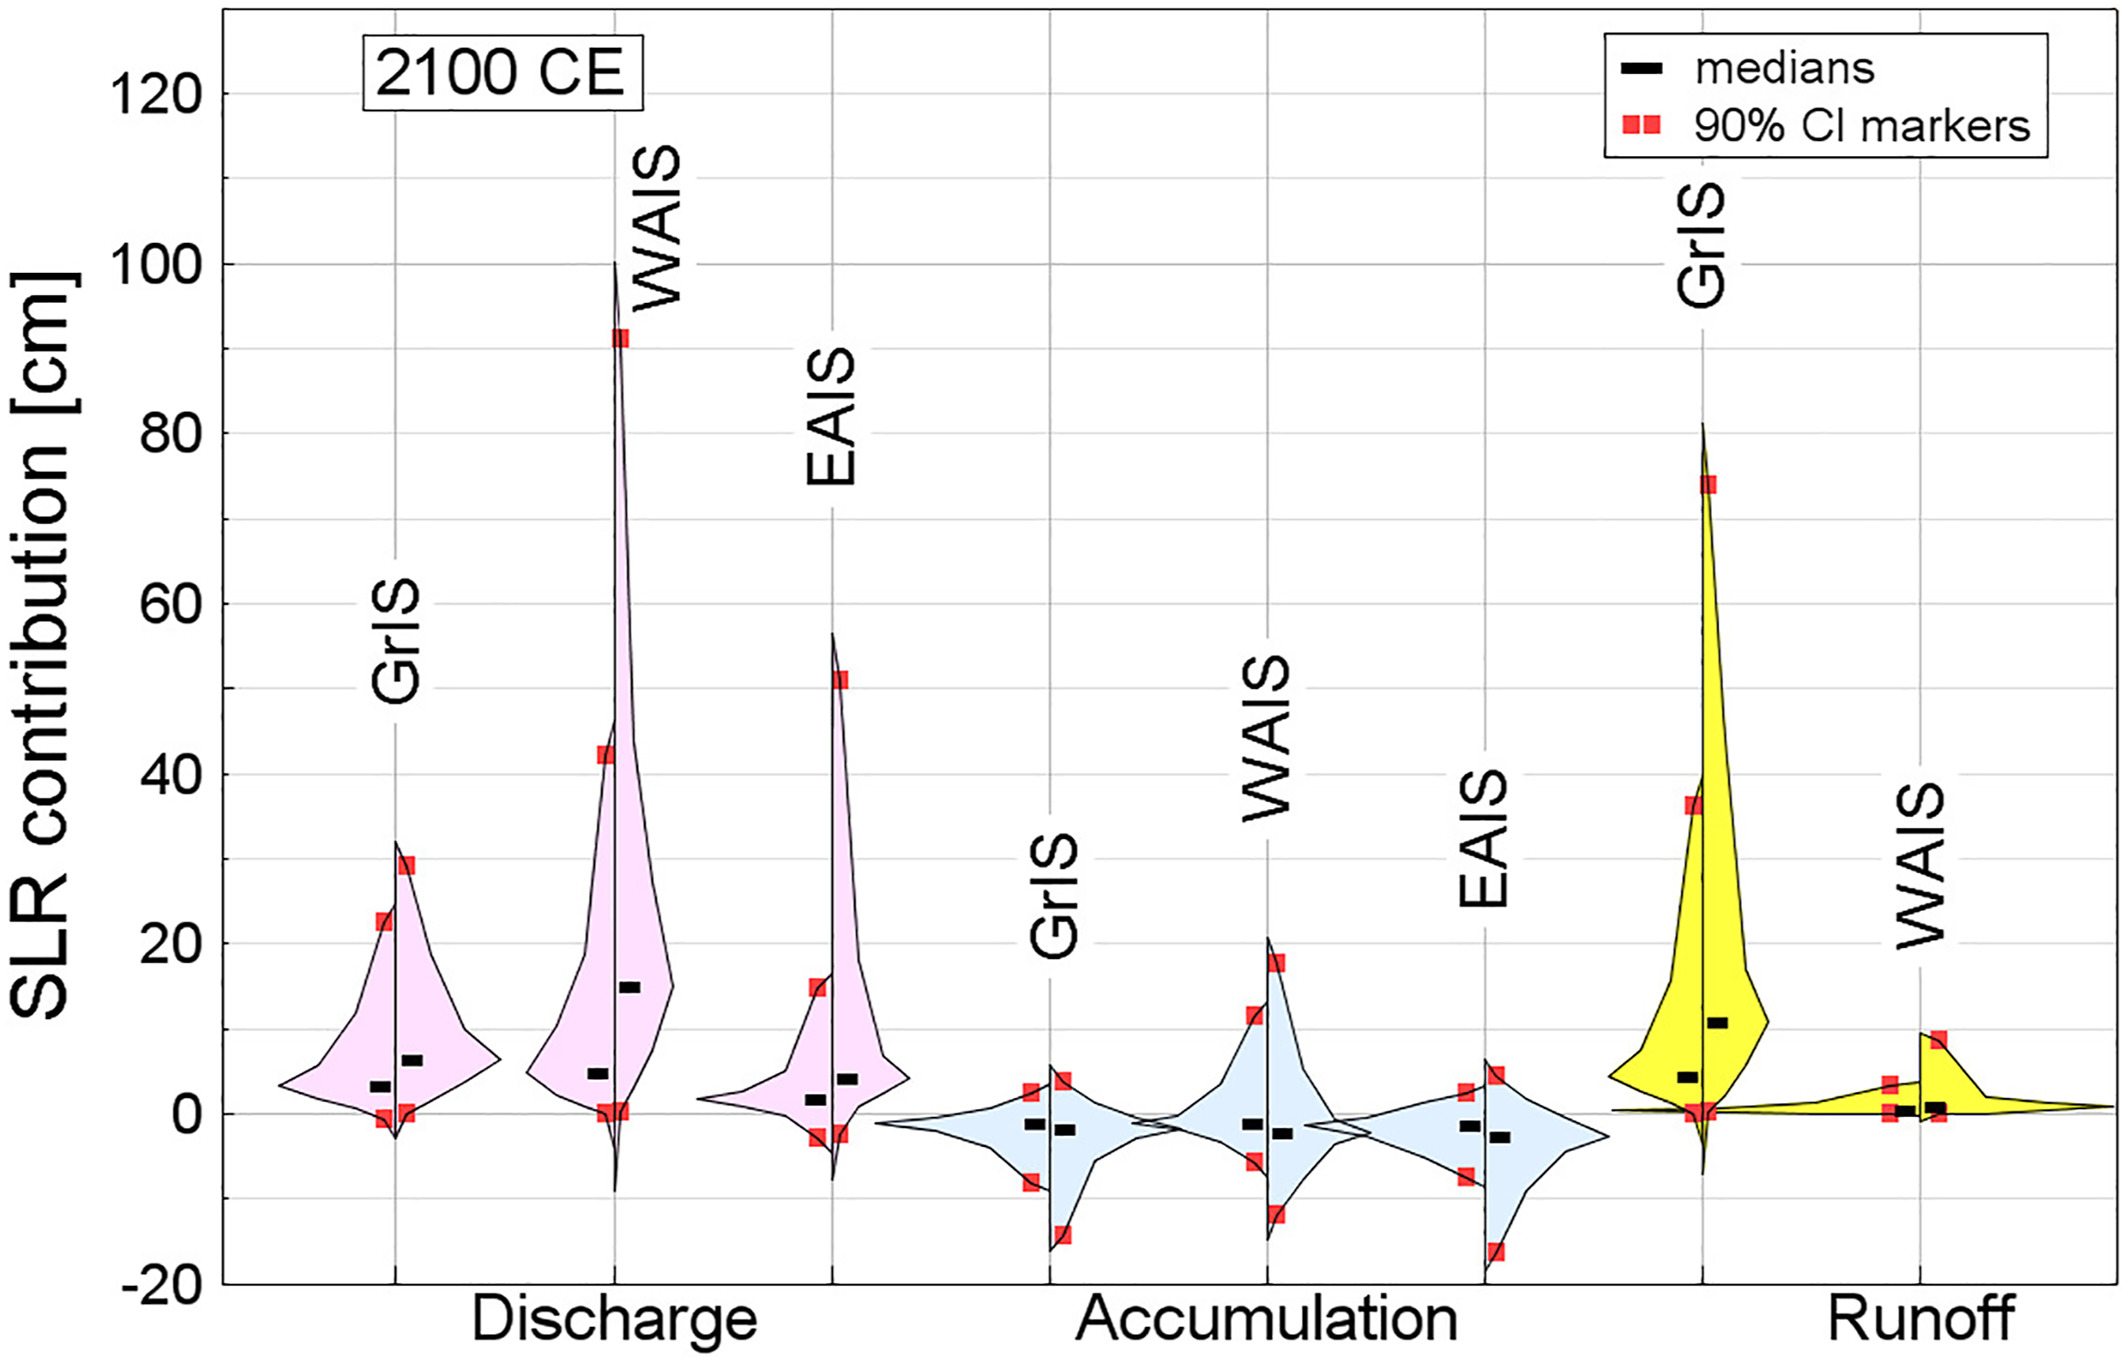
\includegraphics[width=.6\textwidth]{figures/chp1/bamber2022_SLR_uncertainty.jpg}
%     \caption{Probability distributions for projected global sea level rise contributions for the year 2100 from the Greenland Ice Sheet (GrIS), West Antarctic Ice Sheet (WAIS), and East Antarctic Ice Sheet (EAIS), separated into three processes; discharge, accumulation, and runoff. Left and right sides of each distribution show the +2$^{\circ}$C and +5$^{\circ}$C global temperature trajectories, respectively. Figure from \citet{bamberice2022}.}
%     \label{fig:chp1_SLR}
% \end{figure}

\begin{figure}[!ht]
  \centering
    \begin{subfigure}[t]{.54\textwidth}
        \centering
        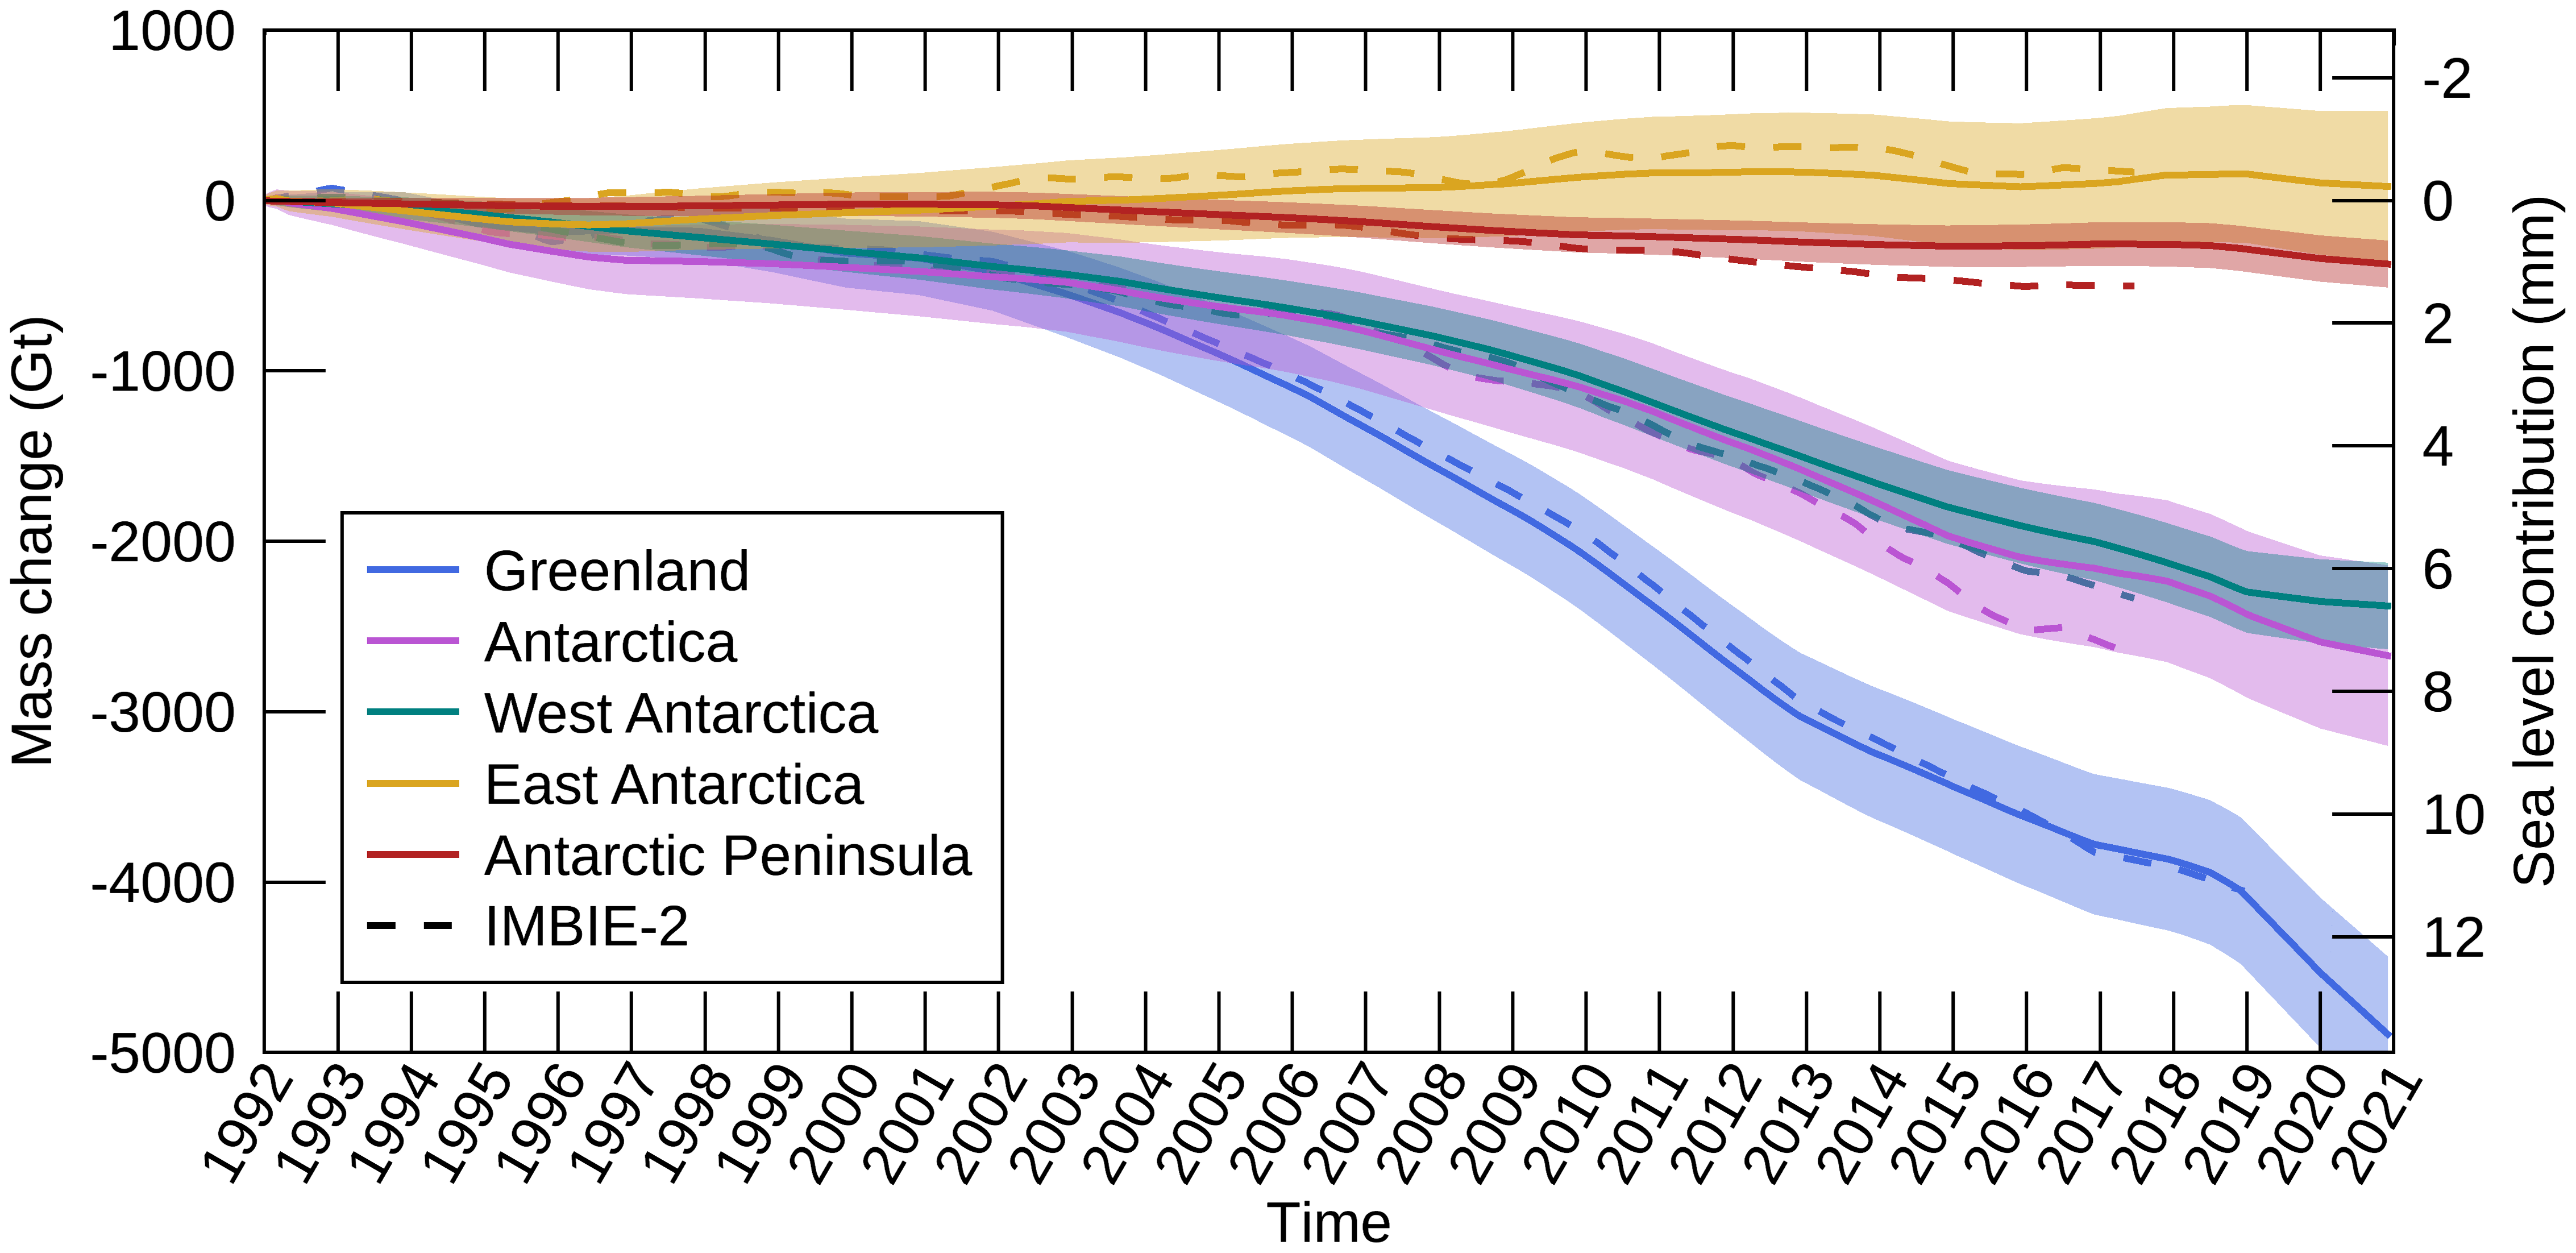
\includegraphics[width=\textwidth]{figures/chp1/Otosaka2023_mass_change.png}
        \caption{}
    \end{subfigure}
    \begin{subfigure}[t]{.44\textwidth}
        \centering
        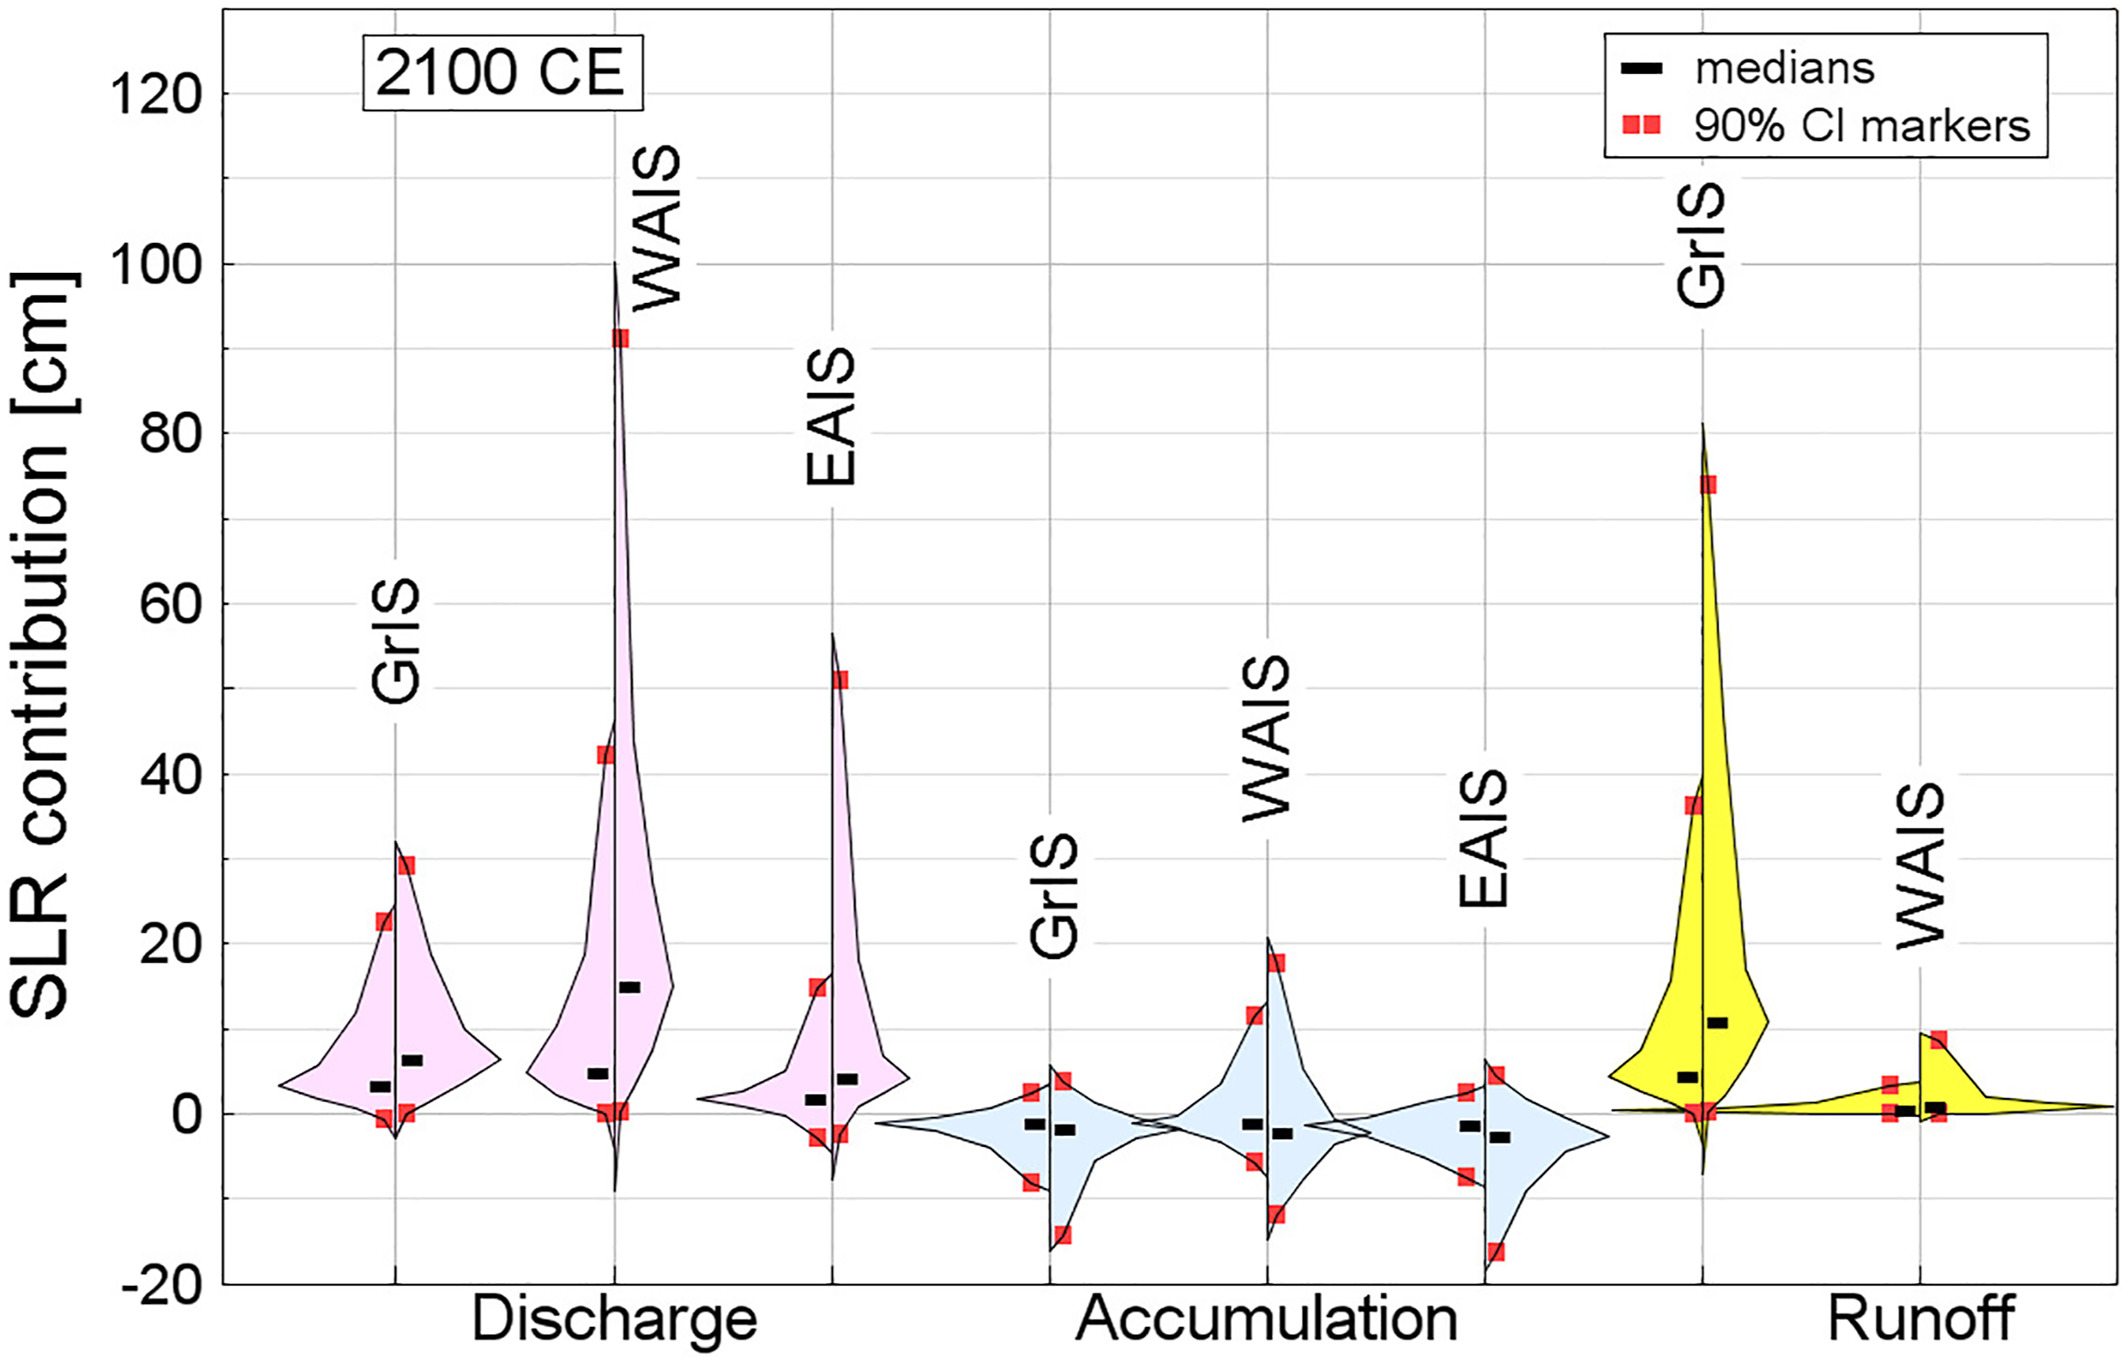
\includegraphics[width=\textwidth]{figures/chp1/bamber2022_SLR_uncertainty.jpg}
        \caption{}
    \end{subfigure}
  \caption[Past observations and future predictions of sea level rise]{Past observations and future predictions of sea level rise.
  \textbf{a)} Observed cumulative mass change and sea level contributions from the various ice sheets. Data comes from satellite-altimetry estimates of volume changes, gravimetric estimates of mass changes, and quantification of input-output fluxes. Figure from \citet{otosakamass2023}.
  \textbf{b)} Probability distributions for projected global sea level rise contributions for the year 2100 from the Greenland Ice Sheet (GrIS), West Antarctic Ice Sheet (WAIS), and East Antarctic Ice Sheet (EAIS), separated into three processes; discharge, accumulation, and runoff. Left and right sides of each distribution show the +2$^{\circ}$C and +5$^{\circ}$C global temperature trajectories, respectively. Figure from \citet{bamberice2022}.}
    \label{fig:chp1_SLR}
\end{figure}

\section[Influences on ice dynamics]{Influence of bathymetry, topography, and geology on ice dynamics\sectionmark{Influences on ice dynamics}}
% \section{Influences on ice dynamics}

The underlying Earth influences ice sheets through several mechanisms, which I group as those resulting from bedrock topography, geologic structures, and bedrock physical properties. Here I describe each of these categories of influences on the Antarctic Ice Sheet, followed by introducing the specific study area, the Ross Ice Shelf.   

\subsection{Bedrock topography}
% confinement / slope controls speed ()
% physiographic steering of ice / water (Holland model 2018, Tinto et al. 2019, halberstadticesheet2016, andersonseismic2019)
% control on erosion / deposition (lee/stoss sides of ridges) (Cuffey and Paterson 2010)
% buttressing of ice shelves ()
% GIA feedbacks (couloncontrasting2021, barlettaobserved2018, kachuckrapid2020)

% we need bathymetry
% how to get bathy (airborne / over-snow radar / over-snow seismics / shipborne seismics)

Offshore bathymetry and onshore bed topography exert several fundamental controls on how the Antarctic Ice Sheet behaves. Offshore, where the ice is floating, the influence of the bathymetry is limited to the guiding of ocean circulations. Bathymetric ridges have been shown to block, or re-direct, the inflow of melt-inducing waters to the ocean cavity beneath floating ice shelves \citep{derydtgeometric2014, zhaosillinfluenced2019, goldbergbathymetric2020}. Approximately 75\% of Antarctica's coastline is composed of these floating ice shelves, and 83\% of total ice discharged into the Southern Ocean from Antarctica is through these shelves, highlighting their significance to Antarctica's ice budget \citep{rignoticeshelf2013}. Of the 83\% of total ice loss from Antarctica through ice shelves, basal melt is responsible for approximately half \citep{greeneantarctic2022, rignoticeshelf2013}. Some of this melt occurs from surface waters, where bathymetry has little effect, but for many of the largest ice shelves, the majority of basal melt occurs along the deep grounding zone \citep{adusumilliinterannual2020}. Here, the melt-inducing water bodies are dense and flow into the ice shelf cavities along the seafloor \citep{hollandmodel2008, tintobathymetry2015}. Therefore, bathymetric features act to guide or block these circulations from reaching the grounding zone where they can melt the ice base. In addition to steering ocean currents, bed topography, in regions of grounded ice, acts to steer the ice flow. \\

As revealed by extensive seismic and swath bathymetry data in Antarctica's Ross Sea (Figure \ref{fig:chp1_data_coverage}a), the dynamics of an advancing or retreating ice sheet are predominantly controlled by the physiography of the bed \citep{halberstadticesheet2016, andersonseismic2019}. If large troughs and banks exist, advancing ice is initially confined by these features, while the banks remain ice-free \citep{andersonross2014}. Eventually, after the ice has covered the entire region, the retreat is initially confined to these narrow troughs, while the banks retain grounded ice for much longer \citep{andersonseismic2019, halberstadticesheet2016}. As the ice thins or retreats into regions of deeper bed topography, these banks remain grounded, while the rest of the ice sheet decouples from the bed, begins floating and forms an ice shelf \citep{shipplate1999}. This remaining grounded ice on bathymetric highs forms pinning points. \\

\begin{figure}[!ht]
    \centering
    \includesvg[inkscapelatex=false,width=0.98\textwidth]{chp1/data_coverage}
    \caption[Summary of existing geologic and geophysical data for Antarctica]{Summary of existing geologic and geophysical data for Antarctica. \textbf{a)} Map of data coverage in Antarctica indicating outcropping regions, drill core sites, seismic and  magnetotelluric surveys, and bed elevation data points of Bedmap3, mostly from airborne radio-echo sounding \citep{frémandantarctic2022}. \textbf{b)} Various methods of acquiring information sub-surface geology. Figure adapted from \citet{aitkenantarctica2023}.}
    \label{fig:chp1_data_coverage}
\end{figure}

Pinning points are regions of locally grounded ice within a floating ice shelf \citep{matsuokaantarctic2015}. The friction between the bed and ice base at these points impart a critical resisting force to the discharge of upstream ice; an effect known as buttressing \citep{thomasice1979, dupontassessment2005}. Since the base of ice shelves is flat relative to the underlying bathymetry, the morphology of the seafloor is the dominant control of the location and geometry of these pinning points. The bedrock topography has been thought to be relatively constant over a millennial timescale, meaning that pinning points' geometries vary mostly by temporal changes in the ice thickness. However, recent studies of glacial isostatic adjustment, the vertical rebound of the Earth following deglaciation, throughout West Antarctica have demonstrated high spatial variability and short (multi-centennial-to-millennial) timescales for these vertical land movements \citep{couloncontrasting2021, barlettaobserved2018, kachuckrapid2020}. As the bedrock beneath portions of West Antarctica continues to rebound, the number and extent of these pinning points will likely increase, possibly providing a stabilizing effect to the ice sheet. \\

All of these above controls on ice dynamics imparted by the physiography of the bed rely on accurate knowledge of bed topography and bathymetry. Due to the inherently challenging nature of Antarctic fieldwork, and the logistical challenge of measuring bed elevations beneath thick ice, 50\% of the Antarctic Ice Sheet is more than 5 km from the nearest measurement of bed elevation \citep[Figure \ref{fig:chp1_data_coverage}a,][]{morlighemdeep2020}. This value increases greatly if the floating ice shelves are included. For grounded ice, the dominant techniques for direct measurements of bed elevation data are airborne radio-echo sounding, over-snow radar, and seismic surveying \citep[Figure \ref{fig:chp1_data_coverage}b,][]{fretwellbedmap22013}. In the open ocean, bathymetry data are typically collected with ship-borne multibeam echo sounding, seismic surveying (Figure \ref{fig:chp1_data_coverage}b), or from satellite-altimetry. Acquiring bathymetry data beneath floating ice shelves presents a particular challenge. The efficient shipborne methods are unavailable since the ice shelves are persistent year-round, unlike the sea ice in the open ocean. Radio-echo sounding, either ground-based or airborne, cannot image through the water column. Direct observations through drilling are possible and exist, but typically require drilling through 100's to 1000's of meters of ice \citep[Figure \ref{fig:chp1_data_coverage},][]{cloughross1979, pattersonsensitivity2022}. Autonomous underwater vehicles (Figure \ref{fig:chp1_data_coverage}b) present another option, but are expensive and have limited range \citep{dowdeswellautonomous2008, nichollsmeasurements2006}. The only feasible method of direct observations of sub-ice shelf bathymetry is over-snow seismic surveying (Figure \ref{fig:chp1_data_coverage}b). However, for the vast area of many ice shelves, even sparse coverage ($\sim50$ km spacing) of seismic points across the ice shelf takes several field seasons of data acquisition \citep{bentleyross1984}. 


\subsection{Geologic structures}
% GHF (larourice2012, pollardsensitivity2005, seroussiinfluence2017)
% GHF, localization from faults (goochpotential2016, begemanspatially2017)
% radiogenic heat from crust (burton-johnsongeothermal2020)
% storage / transport of groundwater (christoffersensignificant2014)
% confinement of water -> increased pore pressure (tulaczykbasal2000, bellwidespread2011)
% enhanced GIA within fault-bound basins (peltierglacial2022, steffenglacially2021)

% we need faults, basement margins, aquifer locations
% how to get this (gravity, magnetics, magnetotellurics)
Additional influences on the overriding ice include the delivery of geothermal heat and subglacial water to the ice base and the vertical deformation of the bedrock in response to changing ice loads. Geothermal heat influences ice dynamics through several mechanisms; 1) increasing the temperature of the ice which lowers its viscosity, leading to  enhanced flow via internal deformation \citep{llubesrelations2006}, 2) meltwater lubrication of the bed reduces friction, enhancing flow \citep{pollardsensitivity2005}, and 3) increasing the ability of the bed to deform via increased pore-fluid pressure, which increases ice flow \citep{tulaczykbasal2000}. The latter two effects, while enhanced by geothermal heat through the melting of ice, also occur with simply the presence of liquid water at the ice-bed interface. As briefly mentioned in the above section, glacial isostatic adjustments of the bedrock following changes in ice load can influence the ice by altering the geometry and locations of grounded ice. \\

Each of these effects; geothermal heat flow, subglacial water availability, and glacial isostatic adjustment, are in turn influenced by geologic structures within the upper crust. A portion of subglacial water comes from either transport along the ice-bed interface, or from the melting of the ice base. However, an often overlooked component of the subglacial hydrologic system is groundwater stored in deep sedimentary aquifers. For example, hydrologic modelling of the ice streams of the Siple Coast (Figure \ref{fig:chp1_data_coverage}a) estimated the components of the hydrologic budget to be 8\% from local basal melting, 47\% from inflow from the ice sheet interior, and 45\% from groundwater reservoirs \citep{christoffersensignificant2014}. These modelling observations of extensive groundwater have been recently verified beneath the Whillans Ice Stream by a magnetotelluric survey. This survey imaged an extensive groundwater aquifer within a sedimentary basin, containing at least an order of magnitude more water than the shallow hydrologic system \citep{gustafsondynamic2022}. The vertical flow of this basinal groundwater is controlled by the pressure of the overriding ice sheet. As this overburden pressure decreases with thinning ice, groundwater is discharged to the ice base \citep{goochpotential2016, lisedimentary2022}. This discharge is likely concentrated along pre-existing weaknesses or impermeable surfaces, such as fault damage zones, or the margins of crystalline basement \citep{joliegeological2021}. During this ice-induced hydraulic unloading, regional geothermal heat is advected along the fluid pathways, leading to potentially highly elevated heat flow delivered to the ice base \citep{ravierglaciohydrogeology2018, lisedimentary2022}. In addition to concentrating both subglacial water and geothermal heat, these faults, or more generically, regions of the crust which have experienced recent faulting, will respond differently to stresses induced by glacial isostatic adjustment. To a first order, the isostatic response of the solid-earth to changing ice load is controlled by the rheology of the mantle \citep{whitehousesolid2019}. However, on a more local scale, pre-existing faults are shown to accommodate glacial isostatic rebound-induced stresses \citep{peltierglacial2022, steffenglacially2021}. \\

To be able to understand the above influences on the ice, we must have some fundamental knowledge of the geologic structures beneath the ice. This includes knowing where sedimentary basins, and possible aquifers within, are located, where faults likely intersect the ice base, and the geometry of the crystalline basement. Each of these components is difficult to image directly. Drilling, seismic surveys, or geologic analysis of rock outcrops all provide valuable information but are not feasible to cover wide regions (Figure \ref{fig:chp1_data_coverage}). Indirect methods are therefore needed. These include techniques such as gravity, magnetic, or electromagnetic methods. Each of these techniques records measurements of the spatial variation of a potential field, such as the Earth's gravity, magnetic, or electromagnetic fields. These fields are all partially dependant on a physical Earth property, such as rock density, magnetic susceptibility, or resistivity. From these relationships, sub-surface geologic information can be modelled. 


\subsection{Basal roughness}
% onset of ice streams (bellinfluence1998, anandakrishnaninfluence1998)
% effective resistance of pinning points (Still mechanical 2019)
% ice streaming (alleydeformation1986, )
% erodibility/deformation of till (alleydeformation1986)

% we need sediment thickness

The last major influence on the ice from the underlying Earth I present is the roughness of the bed which the ice sheet flows over. This bed roughness is important on both a micro and macro scale. At a micro-scale, roughness is determined by the material of which the bed is composed. A bed of erosion-resistance crystalline basement, for example, can greatly hinder the flow of ice. This material results in high friction with the ice base, slowing the sliding of ice \citep{bellinfluence1998}. Conversely, beds composed of fine-grained tills allow fast ice flow. This fast flow is predominantly due to deformation within the till as the ice flows \citep{alleydeformation1986}. In between the end members of crystalline basement and fine grain till are lithified sedimentary rocks, for example. This type of bed may initially lead to high friction with the ice, but due to their high erodability, sedimentary rock will quickly generate till \citep{anandakrishnaninfluence1998}. A macro-scale view of basal roughness is also important for ice dynamics. As observed at the Siple Coast (Figure \ref{fig:chp1_data_coverage}a) ice streams, there is a strong inverse relation between bed roughness, from scales of 5 to >40 km, and ice stream velocities \citep{siegertmacroscale2004}. The composition of the bed also plays an important role in the total effective resistance imparted on ice flow from pinning points \citep{stillmechanical2019}. \\

To best quantify the effect of basal roughness on ice dynamics, information on the material properties of the bed is needed. While sediment samples beneath the ice yield valuable information, they may only represent the bed at the specific location where they were sampled. The most fundamental information needed is the generic rock type of the bed, namely, is the bed loose, unconsolidated sediment, lithified sedimentary rock, or crystalline rock? \citet{aitkenantarctica2023} provide a detailed review of Antarctica's sedimentary basins, and the methods employed to determine both the presence of sediment and the sediment thickness. These methods, as well as the methods described in the above sections, are shown in Figure \ref{fig:chp1_data_coverage}, as reproduced from \citet{aitkenantarctica2023}. 

With the dominant influences from the underlying Earth on ice dynamics laid out, I will now introduce the study area of this thesis, Antarctica's Ross Ice Shelf. 


\section{Ross Ice Shelf}
% what is the RIS? 
% size, location, map
% importance for AIS and SLR
% past fast and large GL retreat

The Ross Ice Shelf is Antarctica's largest ice shelf ($\sim480,000$ km\textsuperscript{2}), Figure \ref{fig:chp1_data_coverage}). It is situated between the Transantarctic Mountains and Marie Byrd Land. It buttresses a catchment of ice that flows from both the East and West Antarctic Ice Sheets. This catchment contains 11.6 m of global sea level equivalent \citep{fretwellbedmap22013, rignotantarctic2011, tintoross2019}. Compared to many other ice shelves, the Ross Ice Shelf is currently relatively stable \citep{moholdtbasal2014, rignoticeshelf2013}. However, geologic evidence from throughout the Ross Sea and the Siple Coast shows that in the past $\sim$7,000 years the shelf has experienced rapid destabilization, disintegration, and large-scale grounding line retreat \citep[e.g.,][]{venturellimid2020, naishobliquitypaced2009}. This major Holocene retreat is thought to have been primarily caused by ocean forcings \citep{lowrydeglacial2019}, as bathymetric troughs guided in the inflow of melt-inducing ocean circulations \citep{tintoross2019}. Once destabilized, the grounding line retreat from the outer continental shelf to the present-day location was controlled primarily by the physiography and geology of the bed \citep{halberstadticesheet2016, andersonseismic2019}. This shows the importance of the underlying Earth's influence on the dynamics of the Ross Ice Shelf. 

% The Ross Ice Shelf sits between the geologically distinct provinces of East and West Antarctica. 
% East Antarctica consists primarily of uniform, thick and stable cratonic crust of Precambrian origins \citep{fitzsimonsreview2000}. 
% Conversely, West Antarctica is the amalgamation of discrete continental blocks with varied and complex histories \citep{jordangeological2020}. 
% These blocks were created or accreted along the paleo-pacific subduction zone. 
% Subduction and much of the associated magmatism waned by the early Cretaceous \citep{siddowaymicroplate2010}, likely leaving the paleo-Ross Embayment region as an elevated and thick section of crust \citep{huertatransition2007, bialasplateau2007}. 
% Subsequently, back-arc extension began, initiating this region's main phase of West Antarctic Rift System extension \citep{siddowaygeology2021}. This distributed extension resulted in over 1000 km of stretching in less than 20 million years () of  and the opening of the Southern Ocean lebreakup of the 
% In the mid-Cretaceous back-arc extension began, leading to the breakup of Gondwana and the formation of the West Antarctic Rift System \cite{jordangeological2020}. 
% Extension with the West Antarctic Rift System 

% this convergent margin was fully transformed into a After this subduction ceased, the convergent margin transistioned into a  

% In general, West Antarctic has.  and has a complex history of,  preconsists predominantly of continental-shield of East Antarctica  is consists of thick cratonic crust, 

% The modern-day geology and physiography of the Ross Ice Shelf region are the result of a long history of geologic, tectonic, and glacial processes. TThe crust of the region

% The Ross Ice Shelf spans a large region of low-lying topography bound to the east and west by mountains. The geologic history of the region is summarized by   covers a region of thhe  Ross Ice Shelf region can be generalized as an extensively thinned and subsided an
% The region is bound to the south and west by the high and steep topography of the Transantarctic Mountains.  to the north by the is The  Figure \ref{fig:chp5_syntheis_figure}


\subsection{Past investigations}
% we stated earlier that bathymetry / basement / ... was fundamental to understanding the geologic interactions with the overriding ice.
% Lit review of RIS data
% what do we still need
%     uncertainty in bathymetry
%     basement topography
%     sediment thickness
%     likely locations of faults and aquifers

By examining various influences on ice dynamics, I identified some key data needed to understand these influences. These data included onshore bed topography, offshore bathymetry, the distribution of sediment, and upper crustal structures such as faults and the topography of the basement. Here, I summarize the history of data collection in the Ross Ice Shelf region specific to these geologic and physiographic features. Geological and geophysical exploration has occurred in the Ross Embayment for over a century. The earliest of these include the 1901-1904 \textit{Discovery} expedition, the 1907-1909 \textit{Nimrod} expedition, and the 1910-1913 \textit{Terra Nova} expedition. These expeditions laid the groundwork of interest in the Ross Embayment from a scientific perspective. The first major survey of the Ross Ice Shelf was part of the 1957-1959 International Geophysical Year traverses. The three over-snow traverses all included a portion of the ice shelf and collected radar, gravity, and seismic data to determine ice thickness, surface elevation, and bed elevation \citep{craryoversnow1959}. These surveys produced early evidence of the extensive below-sea-level bed, thin crust, and distinct geologic provinces throughout West Antarctica \citep{bentleystructure1960}. In the 1970s the Ross Ice Shelf Geophysical and Glaciological Survey \citep[RIGGS,][]{bentleyross1984} consisted of a systematic grid of seismic surveys over the entire ice shelf with an average spacing between survey points of 55 km. After the RIGGS survey, there were a total of $\sim223$ point-source seismic surveys across the ice shelf, all yielding single-point sub-ice shelf bathymetry depths. Of these, eight reported sediment thicknesses beneath. Several faults were hypothesized, based on 2D gravity profiles conducted at many of the stations \citep{greischaranalysis1992}. Since the 1970s, there have been many additional local surveys on the ice shelf, but these have been focused along the grounding zones \citep[e.g.,][]{horganpoststagnation2017, mutobathymetry2013, pattersonsensitivity2022, sternseismic1994, tenbrinkgeophysical1993, wannamakeruplift2017}. The next, and most recent major data-collection campaign on the Ross Ice Shelf was the ROSETTA-ice project. \\

% Scientific cruises to the Ross Sea in the 1970s began to discover the horst - graben nature of the crust, with km's-thick sedimentary basis separated by N-S shallow basement ridges \citep{houtzseismic1973}. Drilling at sites 270, 271, 272, 273 ...

The Ross Ocean and ice Shelf Environment, and Tectonic setting Through Aerogeophysical surveys and modelling project \citep[ROSETTA-ice,][]{tintoross2019}, was a 3-season (2015-2017) airborne geophysical survey of the Ross Ice Shelf. It flew a regular grid of flight lines, with nominal N-S and E-W line spacings of 10 and 55 km, respectively. During each flight, various geophysical data were collected, including ice-penetrating radar, gravity, magnetics and laser altimetry. So far, these ROSETTA-ice data have been used to begin characterizing the geologic nature of the crust \citep{tintoross2019}, to model the depths to the sea floor \citep{tintoross2019}, and to quantify basal melt \citep{dasmulti2020}. \\

Following 60 years of surveying and exploration of the Ross Ice Shelf, our fundamental understanding of the subglacial geology and physiography is still lacking. For an area almost twice the size of New Zealand, we have approximately 8 locations of reported sediment thickness, several hypothesized locations of faults, gaps of over 100 km without bathymetric depths, and limited understanding of our uncertainty in the bathymetry where it has been modelled/interpolated. I propose several research questions which I aim to answer in this thesis.

% What do we know of these sub-RIS geology / physiography characteristics?
%     - low resolution bathymetry
%     - no idea of bathymetry uncertainty
%     - very limited knowledge of sediment distribution
%     - no mapped, or even inferred faults beneath the ice shelf
    
% What are the main knowledge gaps?
%     - don't have accurate bathymetry knowledge
%     - no idea of spatial uncertainty of bathymetry
%     - what are current pinning points composed of? sediment or basement?
% lack of geologic info on RIS, and why it matters

\section{Research questions}
% What are the important geologic controls in the ice for the RIS region?
%     - bathymetry controls basal melt
%     - pinning points, even small ones, control resistive stress
%     - GIA control on retreat / readvance
%     - sediment vital for ice streaming
    
The aim of this thesis is to improve our knowledge of boundary conditions beneath the Ross Ice Shelf in order to better understand the past, present, and future interactions between the ice, ocean, and underlying earth. I aim to accomplish this by answering the following questions:

\begin{enumerate}
    \item 
    What is the geologic structure of the upper crust beneath the Ross Ice Shelf?
    If there are sediments, what is their thickness and distribution? 
    Where are the major faults likely located? 
    \item 
    How can bathymetry beneath an ice shelf best be modelled? 
    Are there further improvements that can be made to the currently employed gravity-inversion process? 
    What are the predominant sources of uncertainty, and how can these be limited? 
    \item 
    How deep is the bathymetry beneath the Ross Ice Shelf and where are we most and least certain about it? 
    \item 
    What are the geologic controls on the Ross Ice Shelf's stability? 
\end{enumerate}

\section{Outline}

This thesis is comprised of five chapters. \\

This chapter, Chapter 1, establishes the context behind the research, introduces the study region, proposes a series of research questions, and contains an outline of this thesis. \\
%It introduces the Ross Embayment region of Antarctica and provides a history of scientific investigations in the region. Additionally, it provides a brief overview of the geophysical exploration methods used throughout the research.

Chapter 2 is adapted from a journal article published in Geophysical Research Letters  \citep{tankersleybasement2022}, reformatted to be included in this thesis. 
It presents a model of the basement topography, and overlying sediment distribution, beneath the Ross Ice Shelf. I use airborne magnetic data from the ROSETTA-ice project, and a depth-to-magnetic source technique to model the sediment-basement contact. This reveals large-scale, fault-controlled extensional basins throughout the sub-Ross Ice Shelf crust. From this, I am able to draw a wide range of inferences on the likely influence of this basement topography on the past, present, and future ice sheet, as well as some tectonic implications. These results provide the first holistic view of the upper crust beneath the Ross Ice Shelf. \\

Chapter 3 details my development of a method to model the depth to the sea floor beneath a floating ice shelf. This method is a gravity inversion, where observations of Earth's gravitational field are used to model bathymetry beneath an ice shelf. I develop open-source Python code with the aim for other researchers to utilize the inversion. I test the inversion against a suite of synthetic and semi-realistic data. This confirms the feasibility of using gravity data to attain bathymetry depths in an Antarctic setting. Additionally, these synthetic tests reveal the relative importance of various aspects of a gravity inversion. These include the importance of \textit{a priori} constraints on the bathymetry, the large errors which can be introduced during the removal of the regional component of gravity, and several suggestions for optimal survey design to minimize error in the resulting bathymetry model. The use of Monte Carlo simulation provides both a spatially variable estimation of uncertainty in the resulting bathymetry and an estimate of the various sources of this uncertainty. \\

Chapter 4 uses the inversion algorithm developed in Chapter 3 to create a new bathymetry model and associated uncertainties beneath the Ross Ice Shelf. The model shows some major differences with past bathymetry models, highlighting areas of the ice shelf that should be carefully considered in future surveys. These include a deeper bathymetric trench along the Transantarctic Mountains, a thicker ocean cavity along a portion of the ice front which may allow the incursion of warm ocean waters and a thicker ocean cavity proximal to the Siple Coast grounding line. My uncertainty analysis shows the region of highest uncertainties is along the Transantarctic Mountain Front. Within this chapter, we perform a comprehensive review of past bathymetry-gravity inversions, for all Antarctic studies, and several Greenland studies. This highlighted some key differences, which I believe I have improved on. \\

Chapter 5 presents a synthesis of the 3 research chapters, and provides a discussion of the research questions. Various future works are suggested and the main conclusions of this thesis are presented. The research chapters in this thesis were written with the intent to publish, including Chapter 2 which is already published. Therefore, I have chosen to keep the style of writing consistent throughout the thesis, with the use of plural possessive pronouns ("we") instead of singular ("I"). 

\section[Data and Code]{Data and Code Availability Statement\sectionmark{Data and Code}} \label{chp1_open_source}

In an effort to adhere to the principles of FAIR scientific investigations, Findability, Accessibility, Interoperability, and Reusability \citep{wilkinsonfair2016}, we have used only open-access data and published all code\footnote{This excludes one component of Chapter \ref{ch:2} which was performed with proprietary software.} used in this thesis. Here we describe where this code and data can be found. All data used from other studies has been cited within each chapter and can be accessed through their respective DOIs. However, most of these datasets were downloaded using the Python package Antarctic-Plots \citep{tankersleyantarctic2023}. I developed this package during this PhD to help with several aspects of conducting research related to Antarctica. See Appendix \ref{appendix:D} for an overview of the capabilities of Antarctic-Plots. Analysis in this study was executed on a computer with an x86\_64 processor with a maximum clock frequency of 2600 MHz with 56 physical cores, 112 logical cores, and 1TB of RAM, using the Operating System Linux-Ubuntu. 

\paragraph*{Chapter \ref{ch:2}}
All of the Python code used to perform the analysis and create the figures of Chapter \ref{ch:2} is available from the following GitHub repository; \url{https://github.com/mdtanker/RIS_basement_sediment}, and the version of the repository used in the published paper is archived at \url{https://doi.org/10.5281/zenodo.6499863} \citep{tankersleymdtanker2022}.

\paragraph*{Chapters \ref{ch:3} \& \ref{ch:4}}
The gravity inversion Python code, the workflow conducted within Jupyter Notebooks, and the creation of all the figures is available from the following GitHub repository; \url{https://github.com/mdtanker/RIS_gravity_inversion} and the version of the repository used in this thesis is archived at \url{https://doi.org/10.5281/zenodo.8084469} \citep{tankersleymdtanker2023}. 

The code for creating the figures in the remainder of this thesis, and the latex files of the thesis itself are available at the following GitHub repository; \url{https://github.com/mdtanker/phdthesis} and is citable with the following DOI; \url{https://doi.org/10.5281/zenodo.8084606}.

\chapter{Airborne magnetic analysis: Basement depths and sediment thickness}
\label{ch:2}
\chaptermark{basement}
% DeepBedMap: a deep neural network for resolving the bed topography of Antarctica

% Macros to follow Copernicus Publications style
% \usepackage{units}
\DeclareRobustCommand*\unit[1]
 {\ensuremath{%
   {\thinmuskip3mu\relax
    \def\mu{\text{\textmu}}\def~{\,}%
    \ifx\f@series\testbx\mathbf{#1}\else\mathrm{#1}\fi}}}
\newcommand\tophline{\hline\noalign{\vspace{1mm}}}
\newcommand\middlehline{\noalign{\vspace{1mm}}\hline\noalign{\vspace{1mm}}}
\newcommand\bottomhline{\noalign{\vspace{1mm}}\hline}

\section*{Abstract}

To resolve the bed elevation of Antarctica, we present DeepBedMap~-- a novel machine learning method that can produce Antarctic bed topography with adequate surface roughness from multiple remote sensing data inputs.
The super-resolution deep convolutional neural network model is trained on scattered regions in Antarctica where high-resolution (250\,\unit{m}) ground-truth bed elevation grids are available.
This model is then used to generate high-resolution bed topography in less surveyed areas.
DeepBedMap improves on previous interpolation methods by not restricting itself to a low-spatial-resolution (1000\,\unit{m}) BEDMAP2 raster image as its prior image.
It takes in additional high-spatial-resolution datasets, such as ice surface elevation, velocity and snow accumulation, to better inform the bed topography even in the absence of ice thickness data from direct ice-penetrating-radar surveys.
The DeepBedMap model is based on an adapted architecture of the Enhanced Super-Resolution Generative Adversarial Network, chosen to minimize per-pixel elevation errors while producing realistic topography.
The final product is a four-times-upsampled (250\,\unit{m}) bed elevation model of Antarctica that can be used by glaciologists interested in the subglacial terrain and by ice sheet modellers wanting to run catchment- or continent-scale ice sheet model simulations.
We show that DeepBedMap offers a rougher topographic profile compared to the standard bicubically interpolated BEDMAP2 and BedMachine Antarctica and envision it being used where a high-resolution bed elevation model is required.

\section{Introduction} %% \introduction[modified heading if necessary]

The bed of the Antarctic ice sheet is one of the most challenging surfaces on Earth to map due to the thick layer of ice cover.
Knowledge of bed elevation is however essential for estimating the volume of ice currently stored in the ice sheets and for input to the numerical models that are used to estimate the contribution ice sheets are likely to make to sea level in the coming century.
The Antarctic ice sheet is estimated to hold a sea level equivalent (SLE) of 57.9\,$\pm$\,0.9\,\unit{m} \citep{MorlighemDeepglacialtroughs2019}.
Between 2012 and 2017, the Antarctic ice sheet was losing mass at an average rate of 219\,$\pm$\,\SI{43}{\giga\tonne\per\year} (0.61\,$\pm$\,\SI{0.12}{\milli\metre\per\year} SLE), with most of the ice loss attributed to the acceleration, retreat and rapid thinning of major West Antarctic Ice Sheet outlet glaciers \citep{IMBIEMassbalanceAntarctic2018}.
Bed elevation exerts additional controls on ice flow by routing subglacial water and providing frictional resistance to flow \citep{SiegertMacroscalebedroughness2004}.
Bed roughness, especially at short wavelengths, exerts a frictional force against the flow of ice, making it an important influence on ice velocity \citep{BinghamDiverselandscapesPine2017,FalciniQuantifyingbedroughness2018}.
The importance of bed elevation has led to major efforts to compile bed elevation models of Antarctica, notably with the BEDMAP1 \citep{LytheBEDMAPnewice2001} and BEDMAP2 \citep{FretwellBedmap2improvedice2013} products.
A need for a higher-spatial-resolution digital elevation model (DEM) is also apparent, as ice sheet models move to using sub-kilometre grids in order to quantify glacier ice flow dynamics more accurately \citep{LeBrocqimprovedAntarcticdataset2010,Grahamhighresolutionsyntheticbed2017}.
Finer grids are especially important at the ice sheet's grounding zone on which adaptive mesh refinement schemes have focused \citep[e.g.][]{CornfordAdaptivemeshrefinement2016}, and attention to the bed roughness component is imperative for proper modelling of fast-flowing outlet glaciers \citep{DurandImpactbedrockdescription2011,NiasContrastingmodelledsensitivity2016}.
Here we address the challenge of producing a high-resolution DEM while preserving a realistic representation of the bed terrain's roughness.

Estimating bed elevation directly from geophysical observations primarily uses ice-penetrating-radar methods \citep[e.g.][]{RobinRadioechoexploration1970}.
Airborne radar methods enable reliable along-track estimates with low uncertainty (around the 1\,{\%} level) introduced by imperfect knowledge of the firn and ice velocity structure, with some potential uncertainty introduced by picking the bed return.
Radar-derived bed estimates remain limited in their geographic coverage \citep{FretwellBedmap2improvedice2013} and are typically anisotropic in their coverage, with higher spatial sampling in the along-track direction than between tracks.

To overcome these limitations, indirect methods of estimating bed elevation have been developed, and these include inverse methods and spatial statistical methods.
Inverse methods use surface observations combined with glaciological-process knowledge to determine ice thickness \citep[e.g.][]{vanPeltiterativeinversemethod2013}.
A non-linear relationship exists between the thickness of glaciers, ice streams and ice sheets and how they flow \citep{Raymondrelationshipsurfacebasal2005}, meaning one can theoretically use a well-resolved surface to infer bed properties \citep[e.g.][]{Farinottimethodestimateice2009}.
Using surface observation inputs, such as the glacier outline, surface digital elevation models, surface mass balance, surface rate of elevation change, and surface ice flow velocity, various models have been tested in the Ice Thickness Models Intercomparison eXperiment \citep[ITMIX;][]{FarinottiHowaccurateare2017} to determine ice thickness (surface elevation minus bed elevation).
While significant inter-model uncertainties do exist, they can be mitigated by combining several models in an ensemble to provide a better consensus estimate \citep{Farinotticonsensusestimateice2019}.
On a larger scale, the inverse technique has also been applied to the Greenland \citep{MorlighemBedMachinev3Complete2017} and Antarctic \citep{MorlighemDeepglacialtroughs2019} ice sheets, specifically using the mass conservation approach \citep{Morlighemmassconservationapproach2011}.
Spatial statistical methods seek to derive a higher-spatial-resolution bed by applying the topographical likeness of bed features known to great detail in one area to other regions.
For example, the conditional simulation method applied by \citet{GoffConditionalsimulationThwaites2014} is able to resolve both fine-scale roughness and channelized morphology over the complex topography of Thwaites Glacier and make use of the fact that roughness statistics are different between highland and lowland areas.
\citet{Grahamhighresolutionsyntheticbed2017} uses a two-step approach to generate their synthetic high-resolution grid, with the high-frequency roughness component coming from the ICECAP and BEDMAP1 compilation radar point data and the low-frequency component coming from BEDMAP2.
Neither method is perfect, and we see all of the above methods as complementary.

We present a deep-neural-network method that is trained on direct ice-penetrating-radar observations over Antarctica and one which has features from both the indirect inverse modelling and spatial statistical methodologies.
An artificial neural network, loosely based on biological neural networks, is a system made up of neurons.
Each neuron comprises a simple mathematical function that takes an input to produce an output value, and neural networks work by combining many of these neurons together.
The term deep neural network is used when there is not a direct function mapping between the input data and final output but two or more layers that are connected to one another \citep[see][for a review]{LeCunDeeplearning2015}.
They are trained using backpropagation, a procedure whereby the weights or parameters of the neurons' connections are adjusted so as to minimize the error between the ground truth and output of the neural network \citep{RumelhartLearningrepresentationsbackpropagating1986}.
Similar work has been done before using artificial neural networks for estimating bed topography\citep[e.g.][]{ClarkeNeuralNetworksApplied2009,MonnierInferencebedtopography2018}, but to our knowledge, no-one so far in the glaciological community has attempted to use convolutional neural networks that work in a more spatially aware, 2-dimensional setting.
Convolutional neural networks differ from standard artificial neural networks in that they use kernels or filters in place of regular neurons \citep[again, see][for a review]{LeCunDeeplearning2015}.
The techniques we employ are prevalent in the computer vision community, having existed since the 1980s \citep{FukushimaNeocognitronnewalgorithm1982,LeCunBackpropagationAppliedHandwritten1989} and are commonly used in visual pattern recognition tasks \citep[e.g.][]{LecunGradientbasedlearningapplied1998,KrizhevskyImageNetClassificationDeep2012}.
Our main contributions are twofold:
we (1)~present a high-resolution (250\,\unit{m}) bed elevation map of Antarctica that goes beyond the 1\,\unit{km} resolution of BEDMAP2 \citep{FretwellBedmap2improvedice2013} and
(2)~design a deep convolutional neural network to integrate as many remote sensing datasets as possible which are relevant to estimating Antarctica's bed topography.
We name the neural network ``DeepBedMap'', and the resulting digital elevation model (DEM) product ``DeepBedMap\_DEM''.


\section{Related Work}

\subsection{Super-Resolution} \label{section:superresolution}

Super resolution involves the processing of a low-resolution raster image into a higher-resolution one \citep{TsaiMultiframeimagerestoration1984}.
The idea is similar to the work on enhancing regular photographs to look crisper.
The problem is especially ill-posed because a specific low-resolution input can correspond to many possible high-resolution outputs, resulting in the development of several different algorithms aimed at solving this challenge \citep[see][for a review]{NasrollahiSuperresolutioncomprehensivesurvey2014}.
One promising approach is to use deep neural networks \citep{LeCunDeeplearning2015} to learn an end-to-end mapping between the low- and high-resolution images, a method coined the Super-Resolution Convolutional Neural Network \citep[SRCNN;][]{DongImageSuperResolutionUsing2014}.
Since the development of SRCNN, multiple advances have been made to improve the perceptual quality of super-resolution neural networks \citep[see][for a review]{YangDeepLearningSingle2019}.
One way is to use a better loss function, also known as a cost function.
A loss function is a mathematical function that represents the error between the output of the neural network and the ground truth (see also Appendix~\ref{appendix:A}).
By having an adversarial component in its loss function, the Super-Resolution Generative Adversarial Network \citep[SRGAN;][]{LedigPhotoRealisticSingleImage2017} manages to produce super-resolution images with finer perceptual details.
A generative adversarial network \citep{GoodfellowGenerativeAdversarialNetworks2014} consists of two neural networks, a generator and a discriminator.
A common analogy used is to treat the generator as an artist that produces imitation paintings and the discriminator as an art critic that determines the authenticity of the paintings.
The artist wants to fool the critic into believing its paintings are real, while the critic tries to identify problems with the painting.
Over time, the artist or generator model learns to improve itself based on the critic's judgement, producing authentic-looking paintings with high perceptual quality.
Perceptual quality is the extent to which an image looks like a valid natural image, usually as judged by a human.
In this case, perceptual quality is quantified mathematically by the discriminator or critic taking into account high-level features of an image like contrast, texture, etc.
Another way to improve performance is by reconfiguring the neural network's architecture, wherein the layout or building blocks of the neural network are changed.
By removing unnecessary model components and adding residual connections \citep{HeDeepResidualLearning2015}, an enhanced deep super-resolution network \citep[EDSR;][]{LimEnhancedDeepResidual2017} features a deeper neural network model that has better performance than older models.
For the DeepBedMap model, we choose to adapt the Enhanced Super-Resolution Generative Adversarial Network \citep[\gls{ESRGAN};][]{WangESRGANEnhancedSuperResolution2019} which brings together the ideas mentioned above.
This approach produces state-of-the-art perceptual quality and won the 2018 Perceptual Image Restoration and Manipulation Challenge on Super Resolution (Third Region; \citealp{Blau2018PIRMChallenge2018}).

\subsection{Network Conditioning} \label{section:networkconditioning}

Network conditioning means having a neural network process one source of information in the context of other sources \citep{DumoulinFeaturewisetransformations2018}.
In a geographic context, conditioning is akin to using not just one layer but also other relevant layers with meaningful links to provide additional information for the task at hand.
Many ways exist to insert extra conditional information into a neural network, such as concatenation-based conditioning, conditional biasing, conditional scaling and conditional affine transformations \citep{DumoulinFeaturewisetransformations2018}.
We choose to use the concatenation-based conditioning approach, whereby all of the individual raster images are concatenated together channel-wise, much like the individual bands of a multispectral satellite image.
This was deemed the most appropriate conditioning method as all the contextual remote sensing datasets are raster grid images and also because this approach aligns with related work in the remote sensing field.

An example similar to this DEM super-resolution problem is the classic problem of pan-sharpening, whereby a blurry low-resolution multispectral image conditioned with a high-resolution panchromatic image can be turned into a high-resolution multispectral image.
There is ongoing research into the use of deep convolutional neural networks for pan-sharpening \citep{MasiPansharpeningConvolutionalNeural2016,ScarpaTargetAdaptiveCNNBasedPansharpening2018}, sometimes with the incorporation of specific domain knowledge \citep{YangPanNetDeepNetwork2017}, all of which show promising improvements over classical image processing methods.
More recently, generative adversarial networks \citep{GoodfellowGenerativeAdversarialNetworks2014} have been used in the conditional sense for general image-to-image translation tasks \citep[e.g.][]{IsolaImagetoImageTranslationConditional2016,ParkSemanticImageSynthesis2019}, and also for producing more realistic pan-sharpened satellite images \citep{LiuPSGANGenerativeAdversarial2018}.
Our DeepBedMap model builds upon these ideas and other related DEM super-resolution work \citep{XuNonlocalsimilaritybased2015,ChenConvolutionalNeuralNetwork2016}, while incorporating extra conditional information specific to the cryospheric domain for resolving the bed elevation of Antarctica.


\section{Data and Methods}

\subsection{Data Preparation} \label{section:datapreparation}

Our convolutional neural network model works on 2-D images, so we ensure all the datasets are in a suitable raster grid format.
Ground-truth bed elevation points picked from radar surveys (see Table~\ref{table:groundtruthdata}) are first compiled together onto a common Antarctic stereographic projection (EPSG:3031) using the WGS84 datum, reprojecting where necessary.
These points are then gridded onto a 250\,\unit{m} spatial resolution (pixel-node-registered) grid.
We preprocess the points first using Generic Mapping Tools v6.0 \citep[GMT6;][]{WesselGenericMappingTools2019}, computing the median elevation for each pixel block in a regular grid.
The preprocessed points are then run through an adjustable-tension continuous-curvature spline function with a tension factor set to 0.35 to produce a digital elevation model grid.
This grid is further post-processed to mask out pixels that are more than 3~\unit{pixels} (750\,\unit{m}) from the nearest ground-truth point.

%T1
\begin{table}[ht]
  \centering
  \footnotesize
  \setlength{\tabcolsep}{5pt}
  \caption[High-resolution ground-truth datasets for training DeepBedMap]{
    High-resolution ground-truth datasets from ice-penetrating-radar surveys (collectively labelled as~$y$) used to train the DeepBedMap model.
    Training site locations can be seen in Fig.~\ref{fig:2}.
  }
  \label{table:groundtruthdata}
  \begin{tabular}{ll}
  \tophline
  Location                        & Citation                                         \\
  \middlehline
  Pine Island Glacier             & \citet{BinghamDiverselandscapesPine2017}         \\
  Wilkes Subglacial Basin         & \citet{JordanHypothesismegaoutburstflooding2010} \\
  Carlson Inlet                   & \citet{KingIcestreamnot2011}                     \\
  Rutford Ice Stream              & \citet{KingSubglaciallandformsRutford2016}       \\
  Various locations in Antarctica & \citet{ShiMultichannelCoherentRadar2010}         \\
  \bottomhline
  \end{tabular}
\end{table}

To create the training dataset, we use a sliding window to obtain square tiles cropped from the high-resolution (250\,\unit{m}) ground-truth bed elevation grids, with each tile required to be completely filled with data (i.e.
no Not a Number -- NaN -- values).
Besides these ground-truth bed elevation tiles, we also obtain other tiled inputs (see Table~\ref{table:datainputs}) corresponding to the same spatial bounding box area.
To reduce border edge artefacts in the prediction, the neural network model's input convolutional layers (see Fig.~\ref{fig:1}) use no padding (also known as ``valid'' padding) when performing the initial convolution operation.
This means that the model input grids ($x$, $w^1$, $w^2$, $w^3$) have to cover a larger spatial area than the ground-truth grids~($y$).
More specifically, the model inputs cover an area of 11\,\unit{km}\,$\times$\,11\,\unit{km} (e.g. 11~\unit{pixels}\,$\times$\,11~\unit{pixels} for BEDMAP2), while the ground-truth grids cover an area of 9\,\unit{km}\,$\times$\,9\,\unit{km} (36~\unit{pixels}\,$\times$\,36~\unit{pixels}).
As the pixels of the ground-truth grids may not align perfectly with those of the model's input grids, we use bilinear interpolation to ensure that all the input grids cover the same spatial bounds as those of the reference ground-truth tiles.
The general locations of these training tiles are shown in orange in Fig.~\ref{fig:2}.

%T2
\begin{landscape}
\vspace*{120pt}
\begin{table*}[ht]
  \small
  \caption{Remote sensing dataset inputs into the DeepBedMap neural network model.}
  \label{table:datainputs}
  \begin{tabular}{lllll}
  \tophline
  Symbol & Name                        & Variable                                           & Spatial resolution           & Citation                                         \\
  \middlehline
  $x$    & BEDMAP2                     & bed elevation (\unit{m})                           & {~~~~~~~}1000\,\unit{m}               & \citet{FretwellBedmap2improvedice2013}           \\
  $w^1$  & REMA                        & surface elevation (\unit{m})                       & {~~~~~~~~~}100\,\unit{m}$^{\mathrm{b}}$ & \citet{HowatReferenceElevationModel2018}         \\
  $w^2$  & MEaSUREs Ice Velocity       & VX, VY (\unit{m\,yr^{-1}})$^{\mathrm{a}}$          & {~~~~~~~~~}500\,\unit{m}$^{\mathrm{c}}$ & \citet{MouginotContinentWideInterferometric2019} \\
  $w^3$  & Antarctic snow accumulation & snow accumulation rate (\unit{kg\,m^{-2}\,yr^{-1}}) & {~~~~~~~}1000\,\unit{m}               & \citet{ArthernAntarcticsnowaccumulation2006}     \\
  \bottomhline
  \end{tabular}
  \caption*{$^{\mathrm{a}}$\,Note that the $x$ and $y$~components of velocity are used here instead of the norm. \\
  $^{\mathrm{b}}$\,Gaps in 100\,\unit{m} mosaic filled in with bilinear resampled 200\,\unit{m} resolution REMA image. \\
  $^{\mathrm{c}}$\,Originally 450\,\unit{m}; bilinear resampled to 500\,\unit{m}.} % Table Footnotes
\end{table*}
\end{landscape}

\subsection{Model Design} \label{section:modeldesign}

%F1
\begin{figure*}[ht]
  \includegraphics[width=\textwidth]{figures/chp2_fig1_deepbedmap_architecture_compressed}
  \caption[DeepBedMap generator model architecture]{
    DeepBedMap generator model architecture composed of three modules.
    The input module processes each of the four inputs (BEDMAP2, \citealp{FretwellBedmap2improvedice2013}; REMA, \citealp{HowatReferenceElevationModel2019}; MEaSUREs Ice Velocity, \citealp{MouginotMEaSUREsPhaseMap2019}; snow accumulation, \citealp{ArthernAntarcticsnowaccumulation2006}; see also Table~\ref{table:datainputs}) into a consistent tensor.
    The core module processes the rich information contained within the concatenated inputs.
    The upsampling module scales the tensor up by 4 times and does some extra processing to produce the output DeepBedMap\_DEM.
  }
  \label{fig:1}
\end{figure*}

Our DeepBedMap model is a generative adversarial network \citep{GoodfellowGenerativeAdversarialNetworks2014} composed of two convolutional neural network models, a generator $G_\theta$ that produces the bed elevation prediction and a discriminator $D_\eta$ critic that will judge the quality of this output.
The two models are trained to compete against each other, with the generator trying to produce images that are misclassified as real by the discriminator and the discriminator learning to spot problems with the generator's prediction in relation to the ground truth.
Following this is a mathematical definition of the neural network models and their architecture.

The objective of the main super-resolution generator model $G_\theta$ is to produce a high-resolution (250\,\unit{m}) grid of Antarctica's bed elevation $\hat{y}$ given a low-resolution (1000\,\unit{m}) BEDMAP2 \citep{FretwellBedmap2improvedice2013} image~$x$.
However, the information contained in BEDMAP2 is insufficient for this regular super-resolution task, so we provide the neural network with more context through network conditioning (see Sect.~\ref{section:networkconditioning}).
Specifically, the model is conditioned at the input block stage with three raster grids (see Table~\ref{table:datainputs}): (1)~ice surface elevation~$w^1$, (2)~ice surface velocity~$w^2$ and (3)~snow accumulation~$w^3$.
This can be formulated as follows:

\begin{equation}\label{eq:1}
  \hat{y} = G_\theta(x, w^1, w^2, w^3),
\end{equation}

where $G_\theta$ is the generator (see Fig.~\ref{fig:1}) that produces high-resolution image candidates~$\hat{y}$.
For brevity in the following equations, we simplify Eq.~(\ref{eq:1}) to hide conditional inputs $w^1, w^2$ and  $w^3$, so that all input images are represented using~$x$.
To train the generative adversarial network, we update the parameters of the generator~$\theta$ and discriminator~$\eta$ as follows:

\begin{align}
  &\hat{\theta} = \arg\min_{\theta} \frac{1}{N}\sum_{n=1}^{N}L_{\mathrm{G}}(\hat{y}_n, y_n), \label{eq:2}\\
  &\hat{\eta} = \arg\min_{\eta} \frac{1}{N}\sum_{n=1}^{N}L_{\mathrm{D}}(\hat{y}_n, y_n), \label{eq:3}
\end{align}

where new estimates of the neural network parameters~$\hat{\theta}$ and~$\hat{\eta}$ are produced by minimizing the total loss functions $L_{\mathrm{G}}$ and $L_{\mathrm{D}}$, respectively, for the generator~$G$ and discriminator~$D$ and $\hat{y}_n$ and $y_n$ are the set of predicted and ground-truth high-resolution images over $N$~training samples.
The generator network's loss~$L_{\mathrm{G}}$ is a custom perceptual loss function with four weighted components~-- content, adversarial, topographic and structural loss.
The discriminator network's loss~$L_{\mathrm{D}}$ is designed to maximize the likelihood that predicted images are classified as fake~(0) and ground-truth images are classified as real~(1).
Details of these loss functions are described in Appendix~\ref{appendix:A}.

Noting that the objective of the Generator $G$ is opposite to that of the Discriminator $D$, we formulate the adversarial min-max problem following \citet{GoodfellowGenerativeAdversarialNetworks2014} as so:

\begin{equation}\label{eq:4}
  \begin{split}
  \min_{G}\,\max_{D} V(G,D) =&~\mathbb{E}_{y \sim P_{\text{data}}(y)}[\ln D(y)]\\
  &+ \mathbb{E}_{x \sim P_{G(x)}}[\ln(1-D(G(x)))],
  \end{split}
\end{equation}

where for the discriminator~$D$, we maximize the expectation~$\mathbb{E}$ or the likelihood that the probability distribution of the discriminator's output fits $D(y)=1$ when $y \sim P_{\text{data}}(y)$; i.e. we want the discriminator to classify the high-resolution image as real (1) when the image~$y$ is in the distribution of the ground-truth images $P_{\text{data}}(y)$.
For the generator~$G$, we minimize the likelihood that the discriminator classifies the generator output $D(G(x))=0$ when $x \sim P_{G(x)}$; i.e. we do not want the discriminator to classify the super-resolution image as fake~(0) when the inputs~$x$ are in the distribution of generated images~$P_{G(x)}$.
The overall goal of the entire network is to make the distribution of generated images~$G(x)$ as similar as possible to the ground truth~$y$ through optimizing the value function~$V$.

%F2
\begin{figure*}[ht]
    \includegraphics[width=\textwidth]{figures/chp2_fig2_deepbedmap_dem_compressed}
    \caption[DeepBedMap\_DEM overview map over the entire Antarctic continent]{
      DeepBedMap\_DEM over the entire Antarctic continent.
      Plotted on an Antarctic stereographic projection (EPSG:3031) with elevation referenced to the WGS84 datum.
      Grounding line is plotted as thin black line.
      Purple box shows Pine Island Glacier extent used in Fig.~\ref{fig:3}.
      Yellow box shows Thwaites Glacier extent used in Fig.~\ref{fig:5}.
      Orange areas show locations of training tiles (see Table~\ref{table:groundtruthdata}).
    }
    \label{fig:2}
\end{figure*}

DeepBedMap's model architecture is adapted from the Enhanced Super-Resolution Generative Adversarial Network
\citep[ESRGAN;][]{WangESRGANEnhancedSuperResolution2019}.
The generator model~$G$ (see Fig.~\ref{fig:1}) consists of an input, core and upsampling module.
The input module is made up of four sub-networks, each one composed of a convolutional neural network that processes the input image into a consistent 9\,$\times$\,9 shaped tensor.
Note that the MEaSUREs Ice Velocity \citep{MouginotMEaSUREsPhaseMap2019} input has two channels, one each for the $x$ and $y$~velocity components.
All the processed inputs are then concatenated together channel-wise before being fed into the core module.
The core module is based on the ESRGAN architecture with 12 residual-in-residual dense blocks \citep[see][for details]{WangESRGANEnhancedSuperResolution2019}, saddled in between a pre-residual and post-residual convolutional layer.
A skip connection runs from the pre-residual layer's output to the post-residual layer's output before being fed into the upsampling module.
This skip connection \citep{HeIdentityMappingsDeep2016} helps with the neural network training process by allowing the model to also consider minimally processed information from the input module, instead of solely relying on derived information from the residual-block layers when performing the upsampling.
The upsampling module is composed of two upsampling blocks, specifically a nearest-neighbour upsampling followed by a convolutional layer and leaky rectified linear unit \citep[\gls{LeakyReLU};][]{MaasRectifiernonlinearitiesimprove2013} activation, which progressively scales the tensors by 2 times each time.
Following this are two deformable convolutional layers \citep{DaiDeformableConvolutionalNetworks2017} which produce the final-output super-resolution DeepBedMap\_DEM.
This generator model is trained to gradually improve its prediction by comparing the predicted output with ground-truth images in the training regions (see Fig.~\ref{fig:2}), using the total loss function defined in Eq.~(\ref{eq:A9}).

The main differences between the DeepBedMap generator model and ESRGAN are the custom input block at the beginning and the deformable convolutional layers at the end.
The custom input block is designed to handle the prior low-resolution BEDMAP2 image and conditional inputs (see Table~\ref{table:datainputs}).
Deformable convolution was chosen in place of the standard convolution so as to enhance the model's predictive capability by having it learn dense spatial transformations.

Besides the generator model, there is a separate adversarial discriminator model $D$ (not shown in the paper).
Again, we follow ESRGAN's \citep{WangESRGANEnhancedSuperResolution2019} lead by implementing the adversarial discriminator network in the style of the Visual Geometry Group convolutional neural network model \citep[VGG;][]{SimonyanVeryDeepConvolutional2014}.
The discriminator model consists of 10 blocks made up of a convolutional, batch normalization \citep{IoffeBatchNormalizationAccelerating2015} and LeakyReLU \citep{MaasRectifiernonlinearitiesimprove2013} layer, followed by two fully connected layers comprised of 100\,\unit{neurons} and 1\,\unit{neuron}, respectively.
For numerical stability, we omit the final fully connected layer's sigmoid activation function from the discriminator model's construction, integrating it instead into the binary cross-entropy loss functions at Eqs.~(\ref{eq:A2}) and~(\ref{eq:A3}) using the log-sum-exp function.
The output of this discriminator model is a value ranging from~0 (fake) to~1 (real) that scores the generator model's output image.
This score is used by both the discriminator and generator in the training process and helps to push the predictions towards more realistic bed elevations.
More details of the neural network training setup can be found in Appendix~\ref{appendix:B}.


\section{Results}

\subsection{DeepBedMap\_DEM Topography} \label{section:deepbedmapdemtopography}

Here we present the output digital elevation model (DEM) of the super-resolution DeepBedMap neural network model and compare it with bed topography produced by other methods.
The resulting DEM has a 250\,\unit{m} spatial resolution and therefore a four-times upsampled bed elevation grid product of BEDMAP2 \citep{FretwellBedmap2improvedice2013}.
In Fig.~\ref{fig:2}, we show that the full Antarctic-wide DeepBedMap\_DEM manages to capture general topographical features across the whole continent.
The model is only valid for grounded-ice regions, but we have produced predictions extending outside of the grounding-zone area (including ice shelf cavities) using the same bed elevation, surface elevation, ice velocity and snow accumulation inputs where such data are available up to the ice shelf front.
We emphasize that the bed elevation under the ice shelves has not been super resolved properly and is not intended for ice sheet modelling use.
Users are encouraged to cut the DeepBedMap\_DEM using their preferred grounding line \citep[e.g.][]{BindschadlerGettingAntarcticanew2011,RignotAntarcticgroundingline2011,MouginotMEaSURESAntarcticBoundaries2017} and replace the under-ice-shelf areas with another bathymetry grid product \citep[e.g.][]{GEBCOCompilationGroupGEBCO2020Grid2020}.
The transition from the DeepBedMap\_DEM to the bathymetry product across the grounding zone can then be smoothed using inverse distance weighting or an alternative interpolation method.

%F3
\begin{figure*}[htbp]
  \includegraphics[width=\textwidth]{figures/chp2_fig3_qualitative_bed_comparison}
  \caption[2-D comparison of interpolated bed elevation grid products over Pine Island Glacier]{
    Comparison of interpolated bed elevation grid products over Pine Island Glacier (see extent in Figure \ref{fig:2}).
    \textbf{a} DeepBedMap (ours) at 250 m resolution.
    \textbf{b} BEDMAP2 \citep{FretwellBedmap2improvedice2013}, originally 1000 m, bicubic interpolated to 250 m.
    \textbf{c} Elevation Difference between DeepBedMap and BEDMAP2.
    \textbf{d} BedMachine Antarctica \citep{MorlighemMEaSUREsBedMachineAntarctica2019}, originally 500 m, bicubic interpolated to 250 m.
  }
  \label{fig:3}
\end{figure*}

%F4
\begin{figure*}[htbp]
  \includegraphics[width=\textwidth]{figures/chp2_fig4_deepbedmap_closeups}
  \caption[2-D Close-up views of DeepBedMap\_DEM over Antarctica]{
    Close-up views of DeepBedMap\_DEM around Antarctica.
    Panels \textbf{(a--c)}~show Siple Coast locations.
    Panels \textbf{(d--f)}~show Weddell Sea region locations.
    Panels \textbf{(g--i)}~show East Antarctica locations.
    Features of interest are annotated in black text against a white background:
    ridges~R, speckle patterns~S, terraces~T, wave patterns~W.
  }
  \label{fig:4}
\end{figure*}

We now highlight some qualitative observations of DeepBedMap\_DEM's bed topography beneath Pine Island Glacier (Figure \ref{fig:3}) and other parts of Antarctica (Figure \ref{fig:4}).
DeepBedMap\_DEM shows a terrain with realistic topographical features, having fine-scale bumps and troughs that makes it rougher than that of BEDMAP2 \citep{FretwellBedmap2improvedice2013} and BedMachine Antarctica \citep{MorlighemMEaSUREsBedMachineAntarctica2019} while still preserving the general topography of the area (Figure \ref{fig:3}).
Over steep topographical areas such as the Transantarctic Mountains (Figure \ref{fig:4}a, \ref{fig:4}h), DeepBedMap produced speckle (\textbf{S}) texture patterns.
Along fast flowing ice streams and glaciers (Figure \ref{fig:4}b, \ref{fig:4}c, \ref{fig:4}d, \ref{fig:4}e, \ref{fig:4}f, \ref{fig:4}g, \ref{fig:4}h), we can see ridges (\textbf{R}) aligned parallel to the sides of the valley, i.e. along flow.
In some cases, the ridges are also oriented perpendicular to the flow direction such at Whillans Ice Stream (Figure \ref{fig:4}b), Bindschadler Ice Stream (Figure \ref{fig:4}c) and Totten Glacier (Figure \ref{fig:4}g), resulting in intersecting ridges that creates a box-like, honeycomb structure.
Over relatively flat regions in both West and East Antarctica (e.g. Figure \ref{fig:4}g), there are some hummocky, wave-like (\textbf{W}) patterns occasionally represented in the terrain.
Terrace (\textbf{T}) features can occasionally be found winding along the side of hills such as at the Gamburtsev Subglacial Mountains (Figure \ref{fig:4}i).


\subsection{Surface Roughness} \label{section:surfaceroughness}

%F5
\begin{figure*}[htbp]
  \includegraphics[width=\textwidth]{figures/chp2_fig5_elevation_roughness_grids}
  \caption[Spatial 2-D view of bed elevation and roughness grids over Thwaites Glacier]{
    Spatial 2-D view of grids over Thwaites Glacier, West Antarctica.
    Plotted on an Antarctic stereographic projection (EPSG:3031) with elevation and SD values in metres referenced to the WGS84 datum.
    \textbf{(a)}~DeepBedMap digital elevation model.
    \textbf{(b)}~2-D roughness from the DeepBedMap\_DEM grid.
    \textbf{(c)}~2-D roughness from interpolated Operation IceBridge grid.
    \textbf{(d)}~2-D roughness from bicubically interpolated BedMachine Antarctica grid.
    Orange points in~\textbf{(a)} correspond to transect sampling locations used in Fig.~\ref{fig:6}.
  }
  \label{fig:5}
\end{figure*}

We compare the roughness of DeepBedMap\_DEM vs. BedMachine Antarctica with ground-truth grids from processed Operation IceBridge data \citep{ShiMultichannelCoherentRadar2010} using standard deviation \gls{SD} as a simple measure of roughness \citep{RippinBasalroughnessInstitute2014}.
We calculate the surface roughness for a single 250\,\unit{m} pixel from the SD of elevation values over a square 1250\,\unit{m}\,$\times$\,1250\,\unit{m} area (i.e. 5~\unit{pixels}\,$\times$\,5~\unit{pixels}) surrounding the central pixel.
Focusing on Thwaites Glacier, the spatial 2-D view of the DeepBedMap\_DEM (Fig.~\ref{fig:5}a) shows a range of typical topographic features such as hills and canyons.
The calculated 2-D roughnesses for both DeepBedMap\_DEM (Fig.~\ref{fig:5}b) and the Ground truth (Fig.~\ref{fig:5}c) lie in a similar range from 0 to 400\,\unit{m}, whereas the roughness of BedMachine Antarctica (Fig.~\ref{fig:5}d) is mostly in the 0-to-200\,\unit{m} range (hence the different colour scale).
Also, the roughness pattern for both DeepBedMap\_DEM and the ground truth has a more distributed cluster pattern made up of little pockets (especially towards the coastal region on the left; see Fig.~\ref{fig:5}b and~c), whereas the BedMachine Antarctica roughness pattern shows larger cluster pockets in isolated regions (see Fig.~\ref{fig:5}d).

Taking a 1-D transect over the 250\,\unit{m} resolution DeepBedMap\_DEM, BedMachine Antarctica and ground-truth grids, we illustrate the differences in bed topography and roughness from the coast towards the inland area of Thwaites Glacier with a flight trace from Operation IceBridge (see Fig.~\ref{fig:6}).
For better comparison, we have calculated the Operation IceBridge ground-truth bed elevation and roughness values from a resampled 250\,\unit{m} grid instead of using its native along-track resolution.
All three elevation profiles are shown to follow the same general trend from the relatively rough coastal region (Fig.~\ref{fig:6}a from $-$1550 to $-$1500\,\unit{km} on the $x$~scale), along the retrograde slope (Fig.~\ref{fig:6}a from $-$1500 to $-$1450\,\unit{km} on the $x$~scale) and into the interior region.
DeepBedMap\_DEM features a relatively noisy elevation profile with multiple fine-scale ($<$\,10\,\unit{km}) bumps and troughs similar to the ground truth, while BedMachine Antarctica shows a smoother profile that is almost a moving average of the ground-truth elevation (Fig.~\ref{fig:6}a).
Looking at the roughness statistic (Fig.~\ref{fig:6}b), both the DeepBedMap\_DEM and Operation IceBridge ground-truth grids have a mean SD of about 40\,\unit{m}, whereas BedMachine Antarctica has a mean of about 10\,\unit{m} and rarely exceeds a SD value of 20\,\unit{m} along the transect.

%F6
\begin{figure}[htbp]
  \includegraphics[width=\textwidth]{figures/chp2_fig6_elevation_roughness_transect}
  \caption[Transect plots of bed elevation and surface roughness of interpolated grid products]{
    Comparing bed elevation~\textbf{(a)} and surface roughness~\textbf{(b)} (SD of elevation values) of each interpolated grid product (250\,\unit{m} resolution) over a transect (see Fig.~\ref{fig:5} for location of transect line).
    Purple values are from the super-resolution DeepBedMap\_DEM;
    orange values are from tension-spline-interpolated Operation IceBridge ground-truth points;
    green values are from bicubically interpolated BedMachine Antarctica.
  }
  \label{fig:6}
\end{figure}


\clearpage
\section{Discussion}

\subsection{Bed Features}

In Sect.~\ref{section:deepbedmapdemtopography}, we show that the DeepBedMap model has produced a high-resolution (250\,\unit{m}) result (see Fig.~\ref{fig:3}) that can capture a detailed picture of the underlying bed topography.
The fine-scale bumps and troughs are the result of the DeepBedMap generator model learning to produce features that are similar to those found in the high-resolution ground-truth datasets it was trained on.
However, there are also artefacts produced by the model.
For example, the winding terrace (T, Fig.~\ref{fig:4}) features are hard to explain, and though they resemble eskers \citep{DrewsActivelyevolvingsubglacial2017}, their placement along the sides of hills does not support this view.
Similarly, we are not sure why speckle (S, Fig.~\ref{fig:4}) texture patterns are found over steep mountains, but the lack of high-resolution training datasets likely leads the model to perform worse over these high-gradient areas.

Another issue is that DeepBedMap will often pick up details from the high-resolution ice surface elevation model \citep{HowatReferenceElevationModel2019} input dataset, which may not be representative of the true bed topography.
For example, the ridges (R, Fig.~\ref{fig:4}) found along fast-flowing ice streams and glaciers are likely to be the imprints of crevasses or flow stripes \citep{GlasserLongitudinalsurfacestructures2012} observable from the surface.
An alternative explanation is that the ridges, especially the honeycomb-shaped ones, are rhombohedral moraine deposits formed by soft sediment squeezed up into basal crevasses that are sometimes found at stagnant surging glaciers \citep{Dowdeswellvarietydistributionsubmarine2016,DowdeswellRhombohedralcrevassefillridges2016,SolheimSeafloormorphologyoutside1985}.
We favour the first interpretation as the positions of these bed features coincide with the surface features and also because these ridges are more likely to be eroded away in these fast-flowing ice stream areas.

% \hack{\newpage}

The hummocky wave-like (W) patterns we observe over the relatively flat and slower-flowing areas are likely to result from surface megadune structures \citep{ScambosSnowMegadune2014}.
Alternatively, they may be ribbed or Rogen moraine features that are formed in an orientation transverse to the ice flow direction \citep{HattestrandRibbedmorainesSweden1997,HattestrandRibbedmoraineformation1999}.
While any one of these two explanations may be valid in different regions of Antarctica, we lean towards the conservative interpretation that these features are the result of the DeepBedMap model overfitting to the ice surface elevation data.

\subsection{Roughness}

In Sect.~\ref{section:surfaceroughness}, we quantitatively show that a well-trained DeepBedMap neural network model can produce high roughness values more comparable to the ground truth than those of BedMachine Antarctica.
While the mass conservation technique used by BedMachine Antarctica \citep{MorlighemDeepglacialtroughs2019} improves upon ordinary interpolation techniques such as bicubic interpolation and kriging, its results are still inherently smooth by nature.
The ground-truth grids show that rough areas do exist on a fine scale, and so the high-resolution models we produce should reflect that.

DeepBedMap\_DEM manages to capture much of the rough topography found in the Operation IceBridge ground-truth data, especially near the coast (see Fig.~\ref{fig:6}a, from $-$1550 to $-$1500\,\unit{km} on the $x$~scale) where the terrain tends to be rougher.
Along the retrograde slope (see Fig.~\ref{fig:6}a, from $-$1500 to $-$1450\,\unit{km} on the $x$~scale), several of the fine-scale ($<$\,10\,\unit{km}) bumps and troughs in DeepBedMap\_DEM can be seen to correlate well in position with the ground truth.
In contrast, the cubically interpolated BedMachine Antarctica product lacks such fine-scale ($<$\,10\,\unit{km}) bumps and troughs, appearing as a relatively smooth terrain over much of the transect.
Previous studies that estimated basal shear stress over Thwaites Glacier have found a band of strong bed extending about 80--100\,\unit{km} from the grounding line, with pockets of weak bed interspersed between bands of strong bed further upstream \citep{JoughinBasalconditionsPine2009,SergienkoRegularPatternsFrictional2013}, a pattern that is broadly consistent with the DeepBedMap\_DEM roughness results (see Fig.~\ref{fig:5}b).

In general, DeepBedMap\_DEM produces a topography that is rougher, with SD values more in line with those observed in the ground truth (see Fig.~\ref{fig:6}b).
The roughness values for BedMachine Antarctica are consistently lower throughout the transect, a consequence of the mass conservation technique using regularization parameters that yield smooth results.
We note that the DeepBedMap\_DEM does appear rougher than the ground truth in certain areas.
It is possible to tweak the training regime to incorporate roughness (or any statistical measure) into the loss function (see Appendix~\ref{appendix:A}) to yield the desired surface, and this will be explored in future work (see Sect.~\ref{section:futuredirections}).
Recent studies have stressed the importance of form drag (basal drag due to bed topography) over skin drag (or basal friction) on the basal traction of Pine Island Glacier \citep{BinghamDiverselandscapesPine2017,Kyrke-SmithRelevanceDetailBasal2018}, and the DeepBedMap super-resolution work here shows strong potential in meeting that demand as a high-resolution bed topography dataset for ice sheet modelling studies.

In terms of bed roughness anisotropy, DeepBedMap is able to capture aspects of it from the ground-truth grids by combining (1)~ice flow direction via the ice velocity grid's $x$ and $y$~components \citep{MouginotMEaSUREsPhaseMap2019}, (2)~ice surface aspect via the ice surface elevation grid \citep{HowatReferenceElevationModel2019}, and (3)~the low-resolution bed elevation input \citep{FretwellBedmap2improvedice2013}.
There are therefore inherent assumptions that the topography of the current bed is associated with the current ice flow direction, surface aspect and existing low-resolution BEDMAP2 anisotropy.
Provided that the direction of this surface velocity and aspect is the same as bed roughness anisotropy, as demonstrated in \citet{HolschuhLinkingpostglaciallandscapes2020}, the neural network will be able to recognize it and perform accordingly.
However, if the ice flow direction and surface aspect is not associated with bed anisotropy, then this assumption will be violated and the model will not perform well.

\subsection{Limitations}

The DeepBedMap model is trained only on a small fraction of the area of Antarctica, at less than 0.1\,{\%} of the grounded-ice regions (excluding ice shelves and islands).
This is because the pixel-based convolutional neural network cannot be trained on sparse survey point measurements, nor is it able to constrain itself with track-based radar data.
As the along-track resolution of radar bed picks are much smaller than 250\,\unit{m} pixels, it is also not easy to preserve roughness from radar unless smaller pixels are used.
The topography generated by the model is sensitive to the accuracy of its data inputs (see Tables~\ref{table:groundtruthdata} and \ref{table:datainputs}), and though this is a problem faced by other inverse methods, neural network models like the one presented can be particularly biased towards the training dataset.
Specifically, the DeepBedMap model focuses on resolving short-wavelength features important for sub-kilometre roughness, compared to BedMachine Antarctica \citep{MorlighemDeepglacialtroughs2019} which recovers large-scale features like ridges and valleys well.

An inherent assumption in this methodology is that the training datasets have sampled the variable bed lithology of Antarctica \citep{CoxGeoMAPdatasetAntarctic2018} sufficiently.
This is unlikely to be true, introducing uncertainty into the result as different lithologies may cause the same macroscale bed landscapes to result in a range of surface features.
In particular, the experimental model's topography is likely skewed towards the distribution of the training regions that tend to reside in coastal regions, especially over ice streams in West Antarctica (see Fig.~\ref{fig:2}).
While bed lithology could be used as an input to inform the DeepBedMap model's prediction, it is challenging to find a suitable geological map (or geopotential proxy; \citealp[see e.g.][]{AitkensubglacialgeologyWilkes2014,CoxGeoMAPdatasetAntarctic2018}) for the entire Antarctic continent that has a sufficiently high spatial resolution.
Ideally, the lithological map (categorical or qualitative) would first be converted to a hardness map with an appropriate erosion law and history incorporated (quantitative).
This is because it is easier to train generative adversarial networks on quantitative data (e.g. hardness as a scale from 0 to 10) than on categorical data variables (e.g. sedimentary, igneous or metamorphic rocks); the latter would require a more elaborate model architecture and loss function design.

\subsection{Future directions} \label{section:futuredirections}

The way forward for DeepBedMap is to combine quality datasets gathered by radioglaciology and remote sensing specialists, with new advancements made by the ice sheet modelling and machine learning community.
While care has been taken to source the best possible datasets (see Tables~\ref{table:groundtruthdata} and~\ref{table:datainputs}), we note that there are still areas where more data are needed.
Radio-echo sounding is the best tool available to fill in the data gap, as it provides not only the high-resolution datasets needed for training but also the background coarse-resolution BEDMAP dataset.
Besides targeting radio-echo-sounding acquisitions over a diverse range of bed and flow types, swath reprocessing of old datasets that have that capability \citep{HolschuhLinkingpostglaciallandscapes2020} may be another useful addition to the training set.
The super-resolution DeepBedMap technique can also be applied on bed elevation inputs newer than BEDMAP2 \citep{FretwellBedmap2improvedice2013}, such as the 1000\,\unit{m} resolution DEM over the Weddell Sea \citep{Jeofry1KmBedTopography2017}, the 500\,\unit{m} resolution BedMachine Antarctica dataset \citep{MorlighemMEaSUREsBedMachineAntarctica2019} or the upcoming BEDMAP3.

A way to increase the number of high-resolution ground-truth training data further is to look at formerly glaciated beds.
There are a wealth of data around the margins of Antarctica in the form of swath bathymetry data and also on land in areas like the former Laurentide ice sheet.
The current model architecture does not support using solely ``elevation'' as an input, because it also requires ice elevation, ice surface velocity and snow accumulation data.
In order to support using these paleobeds as training data, one could do one of the following:

\begin{enumerate}
  \item Have a paleo-ice-sheet model that provides these ice surface observation parameters.
  However, continent-scale ice sheet models quite often produce only kilometre-scale outputs, and there are inherent uncertainties with past ice sheet reconstructions that may bias the resulting trained neural network model.

  \item Modularize the neural network model to support different sets of training data.
  One main branch would be trained like a single-image super-resolution problem \citep{YangDeepLearningSingle2019}, where we try to map a low-resolution BEDMAP2 tile to a high-resolution ground-truth image (be it from a contemporary bed, a paleobed or offshore bathymetry).
  The optional conditional branches would then act to support and improve on the result of this naive super-resolution method.
  This design is more complicated to set up and train, but it can increase the available training data by at least an order of magnitude and lead to better results.
\end{enumerate}

From a satellite remote sensing perspective, it is important to continue the work on increasing spatial coverage and measurement precision.
Some of the conditional datasets used such as REMA \citep{HowatReferenceElevationModel2019} and MEaSUREs Ice Velocity \citep{MouginotMEaSUREsPhaseMap2019} contain data gaps which introduce artefacts in the DeepBedMap\_DEM, and those holes need to be patched up for proper continent-wide prediction.
A surface mass balance dataset with sub-kilometre spatial resolution will also prove useful in replacing the snow accumulation dataset \citep{ArthernAntarcticsnowaccumulation2006} used in this work.
As the DeepBedMap model relies on data from multiple sources collected over different epochs, it has no proper sense of time.
Ice elevation change captured using satellite altimeters such as from CryoSat-2 \citep{HelmElevationelevationchange2014}, ICESat-2 \citep{MarkusIceCloudland2017} or the upcoming CRISTAL \citep{KernCopernicusPolarIce2020} could be added as an additional input to better account for temporal factors.

The DeepBedMap model's modular design (see Sect.~\ref{section:modeldesign}) means the different modules (see Fig.~\ref{fig:1}) can be improved on and adapted for future-use cases.
The generator model architecture's input module can be modified to handle new datasets such as the ones suggested above or redesigned to extract a greater amount of information for better performance.
Similarly, the core and upsampling modules which are based on ESRGAN \citep{WangESRGANEnhancedSuperResolution2019} can be replaced with newer, better architectures as the need arises.
The discriminator model which is currently one designed for standard computer vision tasks can also be modified to incorporate glaciology-specific criteria.
For example, the generated bed elevation image could be scrutinized by the discriminator model for valid properties such as topographic features that are aligned with the ice flow direction.
The redesigned neural network model can be retrained from scratch or fine-tuned using the trained weights from DeepBedMap to further improve the predictive performance.
Taken together, these advances will lead to an even more accurate and higher-resolution bed elevation model.


\section{Conclusions}  %% \conclusions[modified heading if necessary]

The DeepBedMap convolutional neural network method presents a data-driven approach to resolve the bed topography of Antarctica using existing data.
It is an improvement beyond simple interpolation techniques, generating high-spatial-resolution (250\,\unit{m}) topography that preserves detail in bed roughness and is adaptable for catchment- to continent-scale studies on ice sheets.
Unlike other inverse methods that rely on some explicit parameterization of ice flow physics, the model uses deep learning to find suitable neural network parameters via an iterative error minimization approach.
This makes the resulting model particularly sensitive to the training dataset, emphasizing the value of densely spaced bed elevation datasets and the need for such sampling over a more diverse range of Antarctic substrate types.
The use of graphical processing units (GPUs) for training and inference allows the neural network method to scale easily, and the addition of more training datasets will allow it to perform better.

The work here is intended not to discourage the usage of other inverse modelling or spatial statistical techniques but to introduce an alternative methodology, with an outlook towards combining each methodology's strengths.
Once properly trained, the DeepBedMap model runs quickly (about 3\,min for the whole Antarctic continent) and produces realistic rough topography.
Combining the DeepBedMap model with more physically based mass conservation inverse approaches \citep[e.g.][]{MorlighemDeepglacialtroughs2019} will likely result in more efficient ways of generating accurate bed elevation maps of Antarctica.
One side product resulting from this work is a test-driven development framework that can be used to measure and compare the performance of upcoming bed terrain models.
The radioglaciology community has already begun to compile a new comprehensive bed elevation and ice thickness dataset for Antarctica, and there have been discussions on combining various terrain interpolation techniques in an ensemble to collaboratively create the new BEDMAP3.


%% The following commands are for the statements about the availability of data sets and/or software code corresponding to the manuscript.
%% It is strongly recommended to make use of these sections in case data sets and/or software code have been part of your research the article is based on.

\section{Code and data availability}

Python code for data preparation, neural network model training and visualization of model outputs is freely available at \url{https://github.com/weiji14/deepbedmap} (last access: 9~August~2020) and at \url{https://doi.org/10.5281/zenodo.3752613} \citep{LeongDeepBedMap2020}.
Neural network model training experiment runs are also recorded at \url{https://www.comet.ml/weiji14/deepbedmap} (last access: 9~August~2020).

The DeepBedMap\_DEM is available from Zenodo at \url{https://doi.org/10.5281/zenodo.3752613}  \citep{LeongDeepBedMap2020}.
The Pine Island Glacier dataset \citep{BinghamDiverselandscapesPine2017} is available on request from Robert Bingham.
The Carlson Inlet dataset \citep{KingIcestreamnot2011} is available on request from Edward King.
Bed elevation datasets from Wilkes Subglacial Basin \citep{FerraccioliAirborneradarbed2018} and Rutford Ice Stream \citep{KingSubglaciallandformsRutford2016} are available from the British Antarctic Survey's Polar Data Centre (\url{https://ramadda.data.bas.ac.uk}, last access: 14~January~2020).
Other Antarctic bed elevation datasets are available from the Center for Remote Sensing of Ice Sheets (\url{https://data.cresis.ku.edu/data/rds}, last access: 15~August~2019) or from the National Snow and Ice Data Center (\url{https://nsidc.org/data/IRMCR2/versions/1}, last access: 15~August~2019).
BEDMAP2 \citep{FretwellBedmap2improvedice2013} and REMA \citep{HowatReferenceElevationModel2018} are available from the Polar Geospatial Center (\url{http://data.pgc.umn.edu}, last access: 30~August~2019).
MEaSUREs Ice Velocity data \citep{MouginotMEaSUREsPhaseMap2019} are available from NSIDC (\url{https://nsidc.org/data/nsidc-0754/versions/1}, last access: 31~August~2019).
Antarctic snow accumulation data \citep{ArthernAntarcticsnowaccumulation2006} are available from the British Antarctic Survey (\url{https://secure.antarctica.ac.uk/data/bedmap2/resources/Arthern_accumulation}, last access: 17~June~2019).


% \authorcontribution{
%   WJL was responsible for data curation, formal analysis, methodology, software, visualization and writing the original draft.
%   HJH was responsible for funding acquisition and supervision.
%   Both authors conceptualized the work and contributed to the reviewing and editing stages of the writing.
% } %% this section is mandatory

\section{Acknowledgements}

We are grateful to Robert Bingham and Edward King for the Pine Island Glacier and Carlson Inlet data and to all the other researchers in the British Antarctic Survey and Operation IceBridge team for providing free access to the high-resolution bed elevation datasets around Antarctica.
A special thanks to Ruzica Dadic for her help in reviewing draft versions of this paper.
This research was funded by the Royal Society of New Zealand's Rutherford Discovery Fellowship (contract RDF-VUW1602), with additional support from the Erasmus+ programme and International Glaciological Society early-career travel award for presenting earlier versions of this work at the 2019 EGU General Assembly and IGS Symposium on Five Decades of Radioglaciology.

Chapter 2, in full, is a reprint of material as it appears in The Cryosphere:
Leong, W. J., \& Horgan, H. J. (2020). DeepBedMap: A deep neural network for resolving the bed topography of Antarctica. \textit{The Cryosphere}, 14(11), 3687–3705. \url{https://doi.org/10.5194/tc-14-3687-2020}.
The paper was edited by Olivier~Gagliardini and reviewed by Martin~Siegert and one anonymous referee.


\chapter{Gravity inversion: a tool for bathymetry modelling}
\label{ch:3}
\chaptermark{inversion}
% Gravity inversion: a tool for bathymetry modelling

\section*{Abstract}

Sub-ice-shelf bathymetry exerts a primary control on the stability of many Antarctic ice shelves through the geometry of pinning points and the guiding of melt-inducing water masses. Collecting sub-ice-shelf bathymetry data using typical polar surveying methods (e.g. seismic surveying or direct observations) can be inefficient, expensive or unfeasible. Gravity inversions provide a more practical alternative, in which observed variations in Earth's gravitational field are used to predict the bathymetry. This chapter describes a gravity inversion algorithm developed specifically for modelling bathymetry. The inversion is tested on a suite of models, created with a combination of synthetic and real bathymetric data. These tests provide the ability to 1) determine the best practices for conducting bathymetric inversions, 2) recognize the limitations of the inversions, and 3) identify where community efforts should be focused for the future of modelling Antarctica's sub-ice-shelf bathymetry. We find that estimating and removing the regional component of gravity prior to the inversion is the largest source of error in the resulting bathymetry model. To address this, we propose procedures to limit this error and provide recommendations on the minimum spatial density of bathymetry constraint points. Additionally, for common airborne gravity survey designs, we find minimizing noise in the  data is more important than collecting closer-spaced data.

\section*{Plain Language Summary}

The shape of the seafloor beneath the floating extensions of the Antarctic Ice Sheet exerts important controls on the ice. Controls include how the seafloor topography (bathymetry) directs the flow of warm water masses which causes melting at the base of the ice, and determines where ice is anchored to the bedrock. Conventional methods of collecting data on bathymetry are ineffective, impractical, or expensive when applied to ice shelves. One alternative method of acquiring sea floor depths is a method called gravity inversion. Variations in bathymetry can be detected by measurements of Earth's gravity over an ice shelf as a result of the difference in density between seawater and the seafloor. Here, we develop a refined technique for performing a gravity inversion and test the method on artificial data to examine its effectiveness and learn which parts of the inversion are most prone to errors. We find that removing the portion of the gravity data that results from deep geologic structures is the largest source of error. To limit the impact of this and other sources of error in the inversion, we suggest researchers focus on collecting as many point measurements of bathymetry depth (from seismic surveys) and attempt to limit the noise in the gravity data as much as possible. 

\paragraph*{Key Points:}
\begin{enumerate}
    \item We present a new constrained geometric gravity inversion algorithm for recovering density contrasts.
    \item Synthetic models show the regional-residual separation of the gravity data prior to inversion is the dominant source of error.
    \item Quality over quantity for gravity data; efforts should be focused on reducing noise not increasing coverage.
\end{enumerate}

\section{Introduction}

In the last two decades, the Antarctic Ice Sheet has experienced significant ice mass loss, averaging 118 billion tons per year, contributing 5.2~mm to sea-level rise \citep{smithpervasive2020}. This mass loss has been concentrated along the coast, where ocean currents are able to bring warm waters in contact with the ice \citep{rignotfour2019}. Much of Antarctica is fringed with floating extensions of the ice sheet, known as ice shelves (Figure \ref{fig:chp3_ice_shelves}). These ice shelves provide a critical buttressing effect on the upstream ice, slowing the flow of ice from the continent into the oceans \citep{dupontassessment2005}. This buttressing results from lateral drag along the margins of the ice shelf and friction between the ice and the bed at pinning points. Thinning of the ice shelves lowers these resistive forces. Due to the cold climate and lack of surface melt, the majority of Antarctic ice shelves’ thinning occurs as basal melt. This basal melt (Figure \ref{fig:chp3_ice_shelves}b) occurs from contact with relatively warm ocean waters, such as circumpolar deep water and high-salinity shelf water (CDW and HSSW) \citep{rignotfour2019, jenkinsobservations2010}.

These deep-lying warm masses of water originate offshore from the ice shelves and thus can only induce basal melting if they circulate under the shelves. A large enough ocean draft, the distance between the ice base and the bathymetry (Figure \ref{fig:chp3_ice_shelves}a), is required for this circulation to be possible. This connection between ocean draft and basal melting is shown by generally low ice shelf basal melt rates for shelves, or sections of shelves, with shallow ocean drafts \citep[e.g.][]{tintoross2019, pritchardantarctic2012}. Additionally, deep bathymetric troughs in regions of otherwise thin drafts, or conversely, bathymetry ridges in regions of thick drafts, can control the incursion of these water masses \citep{st-laurentrole2013, yangbathymetry2021}.

\begin{figure}[!ht]
    \centering
    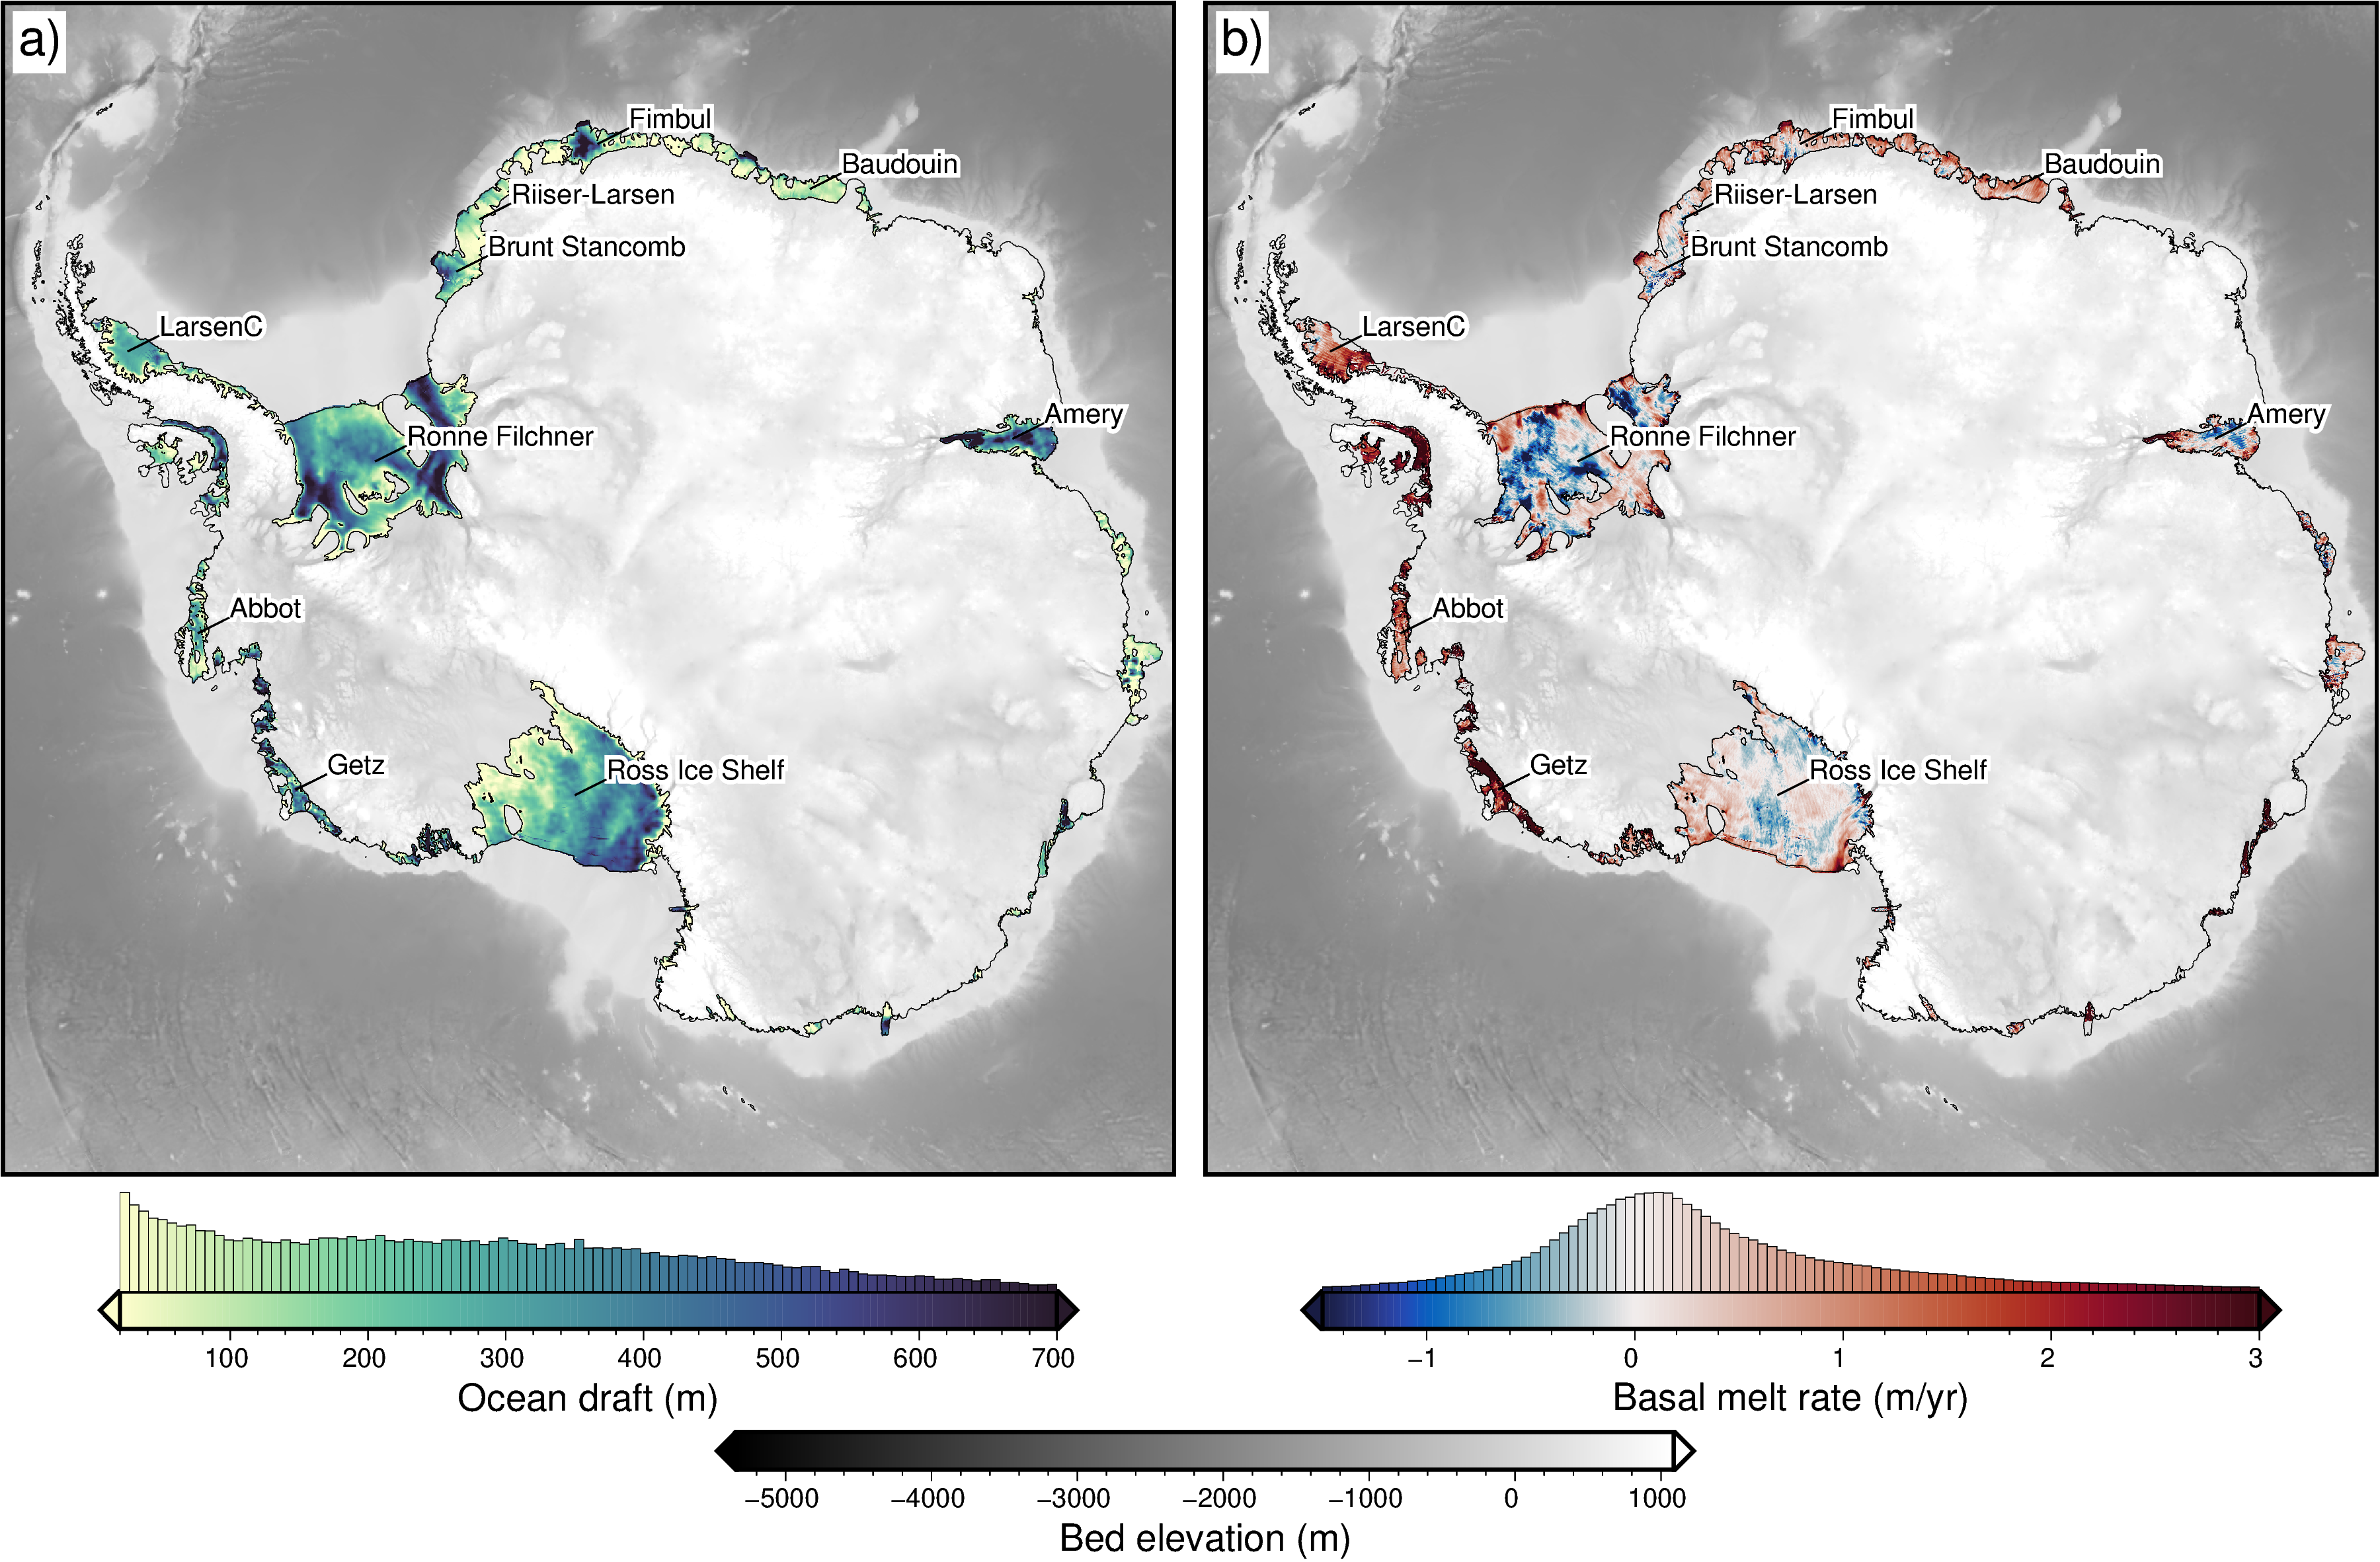
\includegraphics[width=0.95\textwidth]{figures/chp3/chp3_ice_shelves_basal_melt_and_ocean_draft.png}
    \caption[Ice shelves of Antarctica]{Ice shelves of Antarctica. \textbf{a)} Water column thickness beneath the ice shelves from Bedmachine data \citep{morlighemdeep2020, morlighemmeasures2022}. \textbf{b)} Basal melt rate for the ice shelves from \citet{adusumilliinterannual2020}. Both plots show bed elevations in the gray colormap. The 10 largest ice shelves are labelled.}
    \label{fig:chp3_ice_shelves}
\end{figure}

While the elevation of the ice base for many of Antarctica's ice shelves is relatively well-constrained, the water depth is poorly known. The relatively good understanding of the ice base comes from a combination of airborne radar surveys \citep[e.g.][]{dasmulti2020} and satellite altimetry measurements \citep[e.g.][]{griggsantarctic2011}, in conjunction with the hydrostatic equilibrium assumption \citep{bambercomparison1994}. Conversely, there is no equivalent fast and cheap technique to directly survey the bathymetry beneath floating ice shelves. Radar (ground or airborne) cannot image through the thick water, over-ice seismic surveys are slow and expensive, and numerous direct observations through drill holes are impractical. Due to the density contrast between the water and the sediment, the bathymetry surface produces a measurable gravity signal. This signal can be observed from airborne or ground-based gravity surveys, which provides a method, if used correctly, to model sub-shelf bathymetry. This method is a gravity inversion; a geophysical technique to take measurements of an energy source and estimate the physical properties responsible for these measurements \citep[e.g.,][]{oldenburginversion2005, tarantolainverse2005, menkegeophysical2012}. In this case, the energy source is Earth’s gravitational field and the physical Earth property is the depth of the density contrast between the ocean and seafloor. This chapter will first introduce the gravity inversion technique in general, followed by the specific style of gravity inversion, a geometric inversion, which is used here. Next, a suite of synthetic models will be used to assess the performance and limitations of the inversion. The suite of models includes:
\begin{enumerate}
    \item a simple synthetic topography.
    \item a synthetic topography with a regional component of the gravity signal.
    \item a semi-realistic model, using real Antarctic bathymetry and basement topographies to create the synthetic observed gravity. 
\end{enumerate}

With this suite of models, we will test the effects of various levels of noise, the data spacing of the observed gravity, the number of prior constraints, and various inversion methods and parameters. Finally, we will discuss the general limitations of using gravity inversions to recover bathymetry and will provide guidance for conducting gravity inversion for sub-ice-shelf bathymetry. 

\section{Methods}

There are two fundamental types of geophysical modelling, forward modelling, and inverse modelling. Forward modelling is the process of simulating observed data from a model of physical properties. For a gravity application, this may be calculating the gravitational field resulting from a sedimentary basin of a given geometry and/or density model. In general, forward problems are well-posed, meaning there is a unique answer \citep{oldenburginversion2005}. In contrast, inverse modelling, or inversion, is the process of determining physical properties from observed data. For the previous example, this would entail using observed gravity data to predict the sediment thickness of a basin. Inverse problems are generally ill-posed. For a given set of gravity observations, there is a multitude of sedimentary basin configurations which reproduce the observed data with the same degree of accuracy. This is referred to as non-uniqueness and makes geophysical inversions a difficult procedure compared to forward modelling.

\subsection{Geophysical inversion}

In general, inversions consist of three components;

\begin{enumerate}
    \item Forward operator ($f$): This is a mathematical means of linking a physical Earth property to the expected geophysical response. It accomplishes the task of forward modelling, as described above.
    \item Physical property model ($p$): This is a representation of the physical Earth property of interest. While real-world properties are continuous (i.e. a smoothly varying topography), computation often necessitates discretization (i.e. a DEM (digital elevation model), see section \ref{chp3_discretization}). The starting model ($p_0$) typically will include the prior geologic knowledge of the region. To discretize the topography we use a layer of adjacent, vertical right-rectangular prisms.
    \item Fit function ($\phi$): This function describes the similarity between the observed data and the predicted data (resulting from the forward calculation of the property model ($f(p)$)). The goal of the inversion is to minimize this function so that $f(p)$ is as close to the observed data as possible. 
\end{enumerate} 

Here, a mathematical derivation of a generalized discrete inversion problem is shown, following closely to the derivation of \citet{oliveiratopicos2014}. The inversion problem can be framed as finding the set of physical parameters ($\vv{p}$) which when modelled with the forward operator ($f$) produce predicted data ($\vv{d}^{pred}$) as close to the observed data ($\vv{d}^{obs}$), as possible. This inversion is discrete because the topography is represented with a series of grid cells, instead of a continuous function. The difference between the observed and predicted data gives the misfit $\vv{m}$, where 

\begin{equation} \label{eq:misfit}
    \vv{m} \quad = \quad \vv{d}^{obs} - \vv{d}^{pred} \quad = \quad \vv{d}^{obs} - \vv{f}(\vv{p}).
\end{equation}

Here, the $\ell^2$-norm (mean squared error) of the misfit is the metric used to define the \textit{closeness} between the predicted and observed data, where

\begin{equation}
    ||\vv{m}||_2 =  \sqrt{\sum_{i=1}^N [d_i^{obs} - \vv{f_i}(\vv{p})]^2},
\end{equation}

where $N$ is the number of observed data points.

This is defined as the \textit{fit function}, $\phi(\vv{p})$.  The fit function can also be expressed as

\begin{equation}\label{eq:fit_func}
    \phi(\vv{p}) \quad = \quad \vv{m}\cdot\vv{m} \quad = \quad [\vv{d}^{obs} - \vv{f}(\vv{p})]\cdot[\vv{d}^{obs} - \vv{f}(\vv{p})].
\end{equation}
% \begin{equation}\label{eq:fit_func}
%     \phi(\vv{p}) \quad = \quad \vv{m}\cdot\vv{m} \quad = \quad \vv{m}^T\vv{m} \quad = \quad [\vv{d}^{obs} - \vv{f}(\vv{p})]^T [\vv{d}^{obs} - \vv{f}(\vv{p})].
% \end{equation}

In this context, the inversion problem is to determine a vector of parameters $\tilde{p}$ of length $M$ which minimizes $\phi(\vv{p})$. This minimum occurs where the gradient of $\phi(\vv{p})$ at the vector $\tilde{p}$ has zero length.  The gradient of  $\phi(\vv{p})$ evaluated at any $\vv{p}$ is an M-dimensional vector is defined as 
\begin{equation}\label{eq:gradient}
    \nabla\phi(\vv{p}) = \left[\begin{array}{ccc}
    \dfrac{\partial \phi(\vv{p})}{\partial p_{1}}  \\
    \dfrac{\partial \phi(\vv{p})}{\partial p_{2}}  \\
    \vdots \\
    \dfrac{\partial \phi(\vv{p})}{\partial p_{M}} 
\end{array}\right].
\end{equation}

Evaluating the gradient at the i\textsuperscript{th} element, using Equation \ref{eq:fit_func} gives

\begin{equation} \label{eq:partial_deriv_phi}
\begin{aligned}
    \dfrac{\partial \phi(\vv{p})}{\partial p_i} &= 
    \dfrac{\partial}{\partial p_i} \sum_j{
    [d_j^{obs} - f_j(\vv{p})]\cdot[d_j^{obs} - f_j(\vv{p})]
    } \\
    &= \sum_j{\dfrac{\partial}{\partial p_i} 
    [d_j^{obs} - f_j(\vv{p})]\cdot[d_j^{obs} - f_j(\vv{p})]
    } \\
    &= -2\sum_j{\dfrac{\partial f_j(\vv{p})}{\partial p_i}\cdot[d_j^{obs} - f_j(\vv{p})]
    }
\end{aligned}
\end{equation}

Substituting Equation \ref{eq:partial_deriv_phi} into the elements of Equation \ref{eq:gradient} gives

% \begin{equation}
%     \nabla\phi(\vv{p}) = 
%      -2 [\vv{d}^{obs} - \vv{f}(\vv{p})] \times  
%      \left[\begin{array}{ccc}
%         \sum_j{\dfrac{\partial f_j(\vv{p})}{\partial p_1}}  \\
%         \vdots \\
%         \sum_j{\dfrac{\partial f_j(\vv{p})}{\partial p_M}} 
%     \end{array}\right]
% \end{equation}

\begin{equation}
    \nabla\phi(\vv{p}) = 
     -2 \mathbb{J}(\vv{p})  [\vv{d}^{obs} - \vv{f}(\vv{p})],
\end{equation}

\noindent
where $\vv{p}$ is the parameter vector of dimension $M$, $\vv{d}^{obs}$ is the observed data vector of dimension $N$ and $\mathbb{J}$ is the Jacobian matrix of dimension $M \times N$, and is given by

\begin{equation}
\mathbb{J}(\vv{p}) =
\begin{bmatrix}
    \dfrac{\partial f_1(\vv{p})}{\partial p_1} &
        \ldots &
        \dfrac{\partial f_N(\vv{p})}{\partial p_1}
    \\
    \vdots & \ddots & \vdots 
    \\
    \dfrac{\partial f_1(\vv{p})}{\partial p_M} &
        \ldots &
        \dfrac{\partial f_N(\vv{p})}{\partial p_M}
\end{bmatrix}
\label{eq:jacobian}
\end{equation}

Each element of the Jacobian matrix is given by

\begin{equation}
\mathbb{J}_{ij} =
    \dfrac{\partial f_j(\vv{p})}{\partial p_i},
% =
% \begin{bmatrix}
%     \dfrac{\partial f_1}{\partial p_1} &
%         \ldots &
%         \dfrac{\partial f_N}{\partial p_1}
%     \\
%     \vdots & \ddots & \vdots
%     \\
%     \dfrac{\partial f_1}{\partial p_M} &
%         \ldots &
%         \dfrac{\partial f_N}{\partial p_M}
% \end{bmatrix}
\label{eq:jacobian_element}
\end{equation}


% \begin{multline}
%     \dfrac{\partial \phi(\vv{p})}{\partial p_{i}} = 
%     \dfrac{\partial}{\partial p_{i}} \Big\{
%     [\vv{d}^{obs} - \vv{f}(\vv{p})]^T [\vv{d}^{obs} - \vv{f}(\vv{p})]
%     \Big\} \\
%     = 
%     \Bigg\{ -\dfrac{\partial \vv{f}(\vv{p})^T}{\partial p_{i}} [\vv{d}^{obs} - \vv{f}(\vv{p})] \Bigg\} +   
%     \Bigg\{ - [\vv{d}^{obs} - \vv{f}(\vv{p})]^T \dfrac{\partial \vv{f}(\vv{p})}{\partial p_{i}} 
%     \Bigg\} 
% \end{multline}
% which, since the transpose of a scalar is equal to itself, is simplified to

% \begin{equation}\label{eq:partial_deriv_phi}
%     \dfrac{\partial \phi(\vv{p})}{\partial p_{i}} = 
%      -2 \dfrac{\partial \vv{f}(\vv{p})^T}{\partial p_{i}} [\vv{d}^{obs} - \vv{f}(\vv{p})].
% \end{equation}

% Substituting Equation \ref{eq:partial_deriv_phi} into Equation  \ref{eq:gradient} and simplifying gives

% \begin{equation}
%     \nabla\phi(\vv{p}) = -2 \mathbb{J}(\vv{p})^T [\vv{d}^{obs} - \vv{f}(\vv{p})]
% \end{equation}

% where the matrix $\mathbb{J}(\vv{p})$ has dimensions $N \times M$ and is the \textit{Jacobian matrix} of  $\vv{f}(\vv{p})$.

% \begin{equation}
% \mathbb{J}(\vv{p}) =
% \begin{bmatrix}
%     \dfrac{\partial\vv{f}(\vv{p})}{\partial p_1} &
%     \dfrac{\partial\vv{f}(\vv{p})}{\partial p_2} &
%     \ldots &
%     \dfrac{\partial\vv{f}(\vv{p})}{\partial p_M}
% \end{bmatrix}
% =
% \begin{bmatrix}
%     \dfrac{\partial f_1(\vv{p})}{\partial p_1} &
%         \dfrac{\partial f_1(\vv{p})}{\partial p_2} &
%         \ldots &
%         \dfrac{\partial f_1(\vv{p})}{\partial p_M}
%     \\
%     \dfrac{\partial f_2(\vv{p})}{\partial p_1} &
%         \dfrac{\partial f_2(\vv{p})}{\partial p_2} &
%         \ldots &
%         \dfrac{\partial f_2(\vv{p})}{\partial p_M}
%     \\
%     \vdots & \vdots & \ddots & \vdots
%     \\
%     \dfrac{\partial f_N(\vv{p})}{\partial p_1} &
%         \dfrac{\partial f_N(\vv{p})}{\partial p_2} &
%         \ldots &
%         \dfrac{\partial f_N(\vv{p})}{\partial p_M}
% \end{bmatrix}.
% \label{eq:jacobian}
% \end{equation}

\noindent
which is the partial derivative of the j\textsuperscript{th} predicted data with respect to the i\textsuperscript{th} physical parameter. The \textit{Jacobian} ($\mathbb{J}$) is a sensitivity matrix that describes how much the predicted data changes for an infinitesimal change in the physical parameter. For example, let's consider the case of a gravity inversion attempting to recover the density of subsurface cubes. The model consists of 100 cubes, and there are 10 observation points. The Jacobian would be a $100 \times 10$ matrix where $\mathbb{J}_{1,1}$ (the first entry) would be the 1st cube's gravitational derivative with respect to density at the first observation point. The Jacobian, therefore, describes how sensitive each pair of cubes and observations are to a change in density. \\

Once the Jacobian is created, a matrix equation of the form $Ax=b$ is set up, where $A$ is the Jacobian, $x$ is the unknown variable, and $b$ is the data misfit.  
\begin{equation} \label{eq:matrix_eq}
    \mathbb{J} \vv{x} = \vv{m}
\end{equation}

A solution to this linear equation can be found directly, by finding the inverse or pseudo-inverse matrix of the Jacobian, or iteratively via a least-squares solver \citep{jacobygravity2009}. The solution gives the correction which when applied to the physical parameters of interest minimizes the misfit between the observed data and the starting model. 

\subsubsection{Non-Linear inversions}

The derivative of the forward operator with respect to the parameter of interest determines the linearity of an inversion. For a gravity inversion attempting to recover rock density, the derivative of gravity with respect to density is constant, and thus the inversion is considered linear \citep{asterparameter2018}. Conversely, a gravity inversion attempting to recover the depth to a surface, or the thickness of a layer, is non-linear since the vertical derivative of gravity (derivative with respect to depth) is dependent on the depth. Non-linear inversion cannot be solved directly, with matrix inversion \citep{jacobygravity2009}. They must be linearized; which is the purpose of the Jacobian matrix. The Jacobian enables a minimum-norm solution to be found with an iterative solver, where at each iteration, the calculated corrections ($\vv{x}$) are applied to the starting model, the residuals ($\vv{m}$) are recalculated, the Jacobian is updated, and Equation \ref{eq:matrix_eq} is solved again, giving a new set of corrections. This is repeated until $\phi(\vv{p})$ is suitably low.

\subsubsection{Geometric inversions}
Most gravity inversions aim to recover the distributions of densities in the subsurface. For this technique, the model domain is discretized into a series of polygons (for 2D) or polyhedrons (for 3D), and the inversion aims to predict the density of each polygon. This is widely used due to its relevance in mineral exploration \citep{oldenburggeophysical2007}. Less commonly used are gravity inversions which aim to recover the depth, shape, or volume of features. This style of gravity inversions are referred to as geometric inversions. They are typically used to estimate relief of the Moho \citep[e.g][]{uiedafast2017, borghimoho2022} or the sediment-basement contact \citep[e.g.][]{santosefficient2015, barbosagravity2007}. In this chapter, geometric inversions are used to recover the bathymetry. This use case of gravity inversion is unique to studying the cryosphere. In locations without ice cover, bathymetry data is typically collected with shipborne multi-beam echo sounding, airborne LiDAR, or satellite altimetry. 

\subsection{Forward modelling}

To perform a geometric gravity inversion, first, the gravitational field produced by a topographic surface must be able to be calculated. This topography is approximated as a constant density contrast between the overlying and underlying materials. The topography is often modelled as a series of adjacent vertical right-rectangular prisms. For a certain observation point, the gravitational field produced by this layer of prisms is the sum of the forward gravity of each prism. This forward gravity calculation of a prism is accomplished with the analytical solutions given by \citet{nagygravitational2000}, as implemented in the Python package Harmonica \citep{fatiandoaterraprojectharmonica2023}.

\subsubsection{Discretization}\label{chp3_discretization}
There are several options for discretizing a density contrast as a series of prisms (Figure \ref{fig:chp3_discretization}). The most conceptually simple method is for the prisms to represent the true density and geometry of the material on either side of the surface (Figure \ref{fig:chp3_discretization}b). In this method, the topography is represented by the base of the upper prisms, and by the tops of the lower prisms. Alternatively, the contrast can be represented by a layer of prisms either above or below the surface, ending at an arbitrary reference, typically the minimum or maximum value of the surface (Figure \ref{fig:chp3_discretization}c-d). For this, the prism’s density values are relative to the medium on the other side of the surface (i.e. if prisms are below the surface, their densities are $\rho_{below} - \rho_{above}$). The last option is to choose a flat reference surface (typically the mean value of the surface or sea level) and create prisms between this and the surface (Figure \ref{fig:chp3_discretization}e). Prisms above the reference are assigned a positive density contrast ($\Delta{\rho} = \rho_{below} − \rho_{above}$), and prisms below the surface a negative density contrast ($\Delta{\rho} = \rho_{above} − \rho_{below}$). All of these methods result in similar forward gravity calculations. Note that the absolute density option (Figure \ref{fig:chp3_discretization}b) has twice as many prisms as the other options, significantly increasing its computational expense, regardless of whether or not a buffer zone is used.

\begin{figure}[!ht]
    \centering
    \includesvg[inkscapelatex=false,width=0.65\textwidth]{chp3/chp3_discretization}
    \caption[Equivalent methods of discretizing a density contrast]{Equivalent methods of discretizing a density contrast (\textbf{a}) across a surface. \textbf{b)} Use absolute densities of the mediums above and below the reference, with prisms on either side. \textbf{c-d)} Use the density contrast across the surface, with prisms either above or below, and the sign of the density contrast reflecting whether they are above or below. \textbf{e)} Use a reference surface, with prisms above having a positive density contrast and prisms below a negative contrast.}
    \label{fig:chp3_discretization}
\end{figure}

\subsubsection{Gravity edge effects} \label{chp3_edge_effects}
Any forward gravity calculation of a surface will include gravitational edge effects. These effects are typically a decay in the gravitational field towards the edges of the prism model due to the void space (density of 0) beyond the edge of the model. The magnitude of decay is dependent on the average thickness and density of prisms near the edge. Larger or denser prisms create a large contrast with the void space, resulting in a greater amount of decay. Therefore, the absolute density method of discretization (Figure \ref{fig:chp3_discretization}b) produces the largest edge effects due to the high-density values and large total thickness of the prisms. The relative density methods (Figure \ref{fig:chp3_discretization}c-d) produce a smaller edge effect, since the prisms are only above or below the surface, reducing their total thickness. The density values are also less than in the absolute density method. The reference surface method (Figure \ref{fig:chp3_discretization}e) produces the smallest edge effects due to both a) the mean prism thickness being smaller, and b) positive and negative density prisms having opposite edge effects, partially cancelling each other out. This is only applicable if the reference level is located within the range of the values of the surface. Note that with a reference level completely above or below the surface, the reference method becomes identical to methods c) and d) of Figure \ref{fig:chp3_discretization}. \\

A buffer zone can be used to reduce the impact of these edge effects by calculating forward gravity confined to an inner region, while the prism model extends beyond. This limits the majority of the edge effects to outside the region of calculation. Too large of a buffer zone will add an unnecessary amount of computation (more prisms), while too small of a zone will introduce unacceptably large edge effects to the calculations.


\subsection{Isolating anomalies}

For a successful geometric gravity inversion, the component of the observed gravity field resulting from the density contrast of interest must be isolated from all other gravity signals. This section describes the process of isolating the required anomaly. Since this chapter consists of synthetic gravity, the discussion of correcting raw gravity measurements and deriving the various gravity anomalies is omitted. See Chapter \ref{ch:4} for further discussion of gravity data processing. Here, \textit{synthetic observed gravity} is taken to mean the gravity effect resulting solely from deviations between the true synthetic model, and a simple reference model, defined by a flat surface with a constant density above and a constant density below. This is considered a partial topo-corrected gravity disturbance, since the gravity effect of other layers, such as ice and water, if present, is assumed to have been corrected for. The misfit, $\vv{m}$, in Equation \ref{eq:misfit}, is defined as this synthetic observed gravity minus the forward gravity effect of the starting bathymetry. \\

\subsection{Regional vs. Residual gravity} \label{chp3_regional_seperation}

The topography-free gravity disturbance is often simplified as consisting of two components, the regional and residual fields. The regional field typically dominates the signal and is often the result of deeper and broader structures, such as Moho variations. Superimposed on this signal is the residual field, which is typically the result of shallower structures. The terms residual and regional are relative; here, they are taken to mean the gravity effect of the bathymetry versus that of all deeper structures, respectively. In this inversion, the residual, regional, and misfit are related by

\begin{equation} \label{eq:regional_residual}
    \vv{m} = \vv{m}_{res} + \vv{m}_{reg},
\end{equation}

\noindent
where $\vv{m}$ is the overall data misfit, from Equation \ref{eq:misfit}. The residual misfit, $\vv{m}_{res}$, is the desired input into the inversion, and thus the regional component, $\vv{m}_{reg}$, must be removed prior to the inversion. This step proves to be one of the most challenging steps of a bathymetric inversion, especially in areas of limited constraints \citep{brisbourneseabed2014}. Removing an incorrect regional field, whether it is too much or too little, will directly impact the resulting bathymetry results. Regional-residual separation is also highly non-unique and benefits greatly from \textit{a priori} constraints. Many methods of regional separation rely on the simplifying assumption that the regional field consists of longer-wavelength anomalies, while the residual field dominates the short-wavelength components. Here, four methods of estimating the regional component of gravity are described.

\begin{enumerate}
    \item Low-pass filter:
        With the assumption outlined above, a low-pass filter can be used to isolate the regional gravity. For this, a Gaussian wavelength filter is used and the filter width can be varied based on the expected regional anomaly wavelengths. This method requires the data to be gridded over the entire domain, which may be a problem for sparse surveys. or irregularly shaped domains. The choice of wavelength is subjective and needs to be carefully considered. See \citet{eisermannbathymetry2020} for a bathymetry inversion utilizing this method of regional separation. 
    \item Trend removal:
        Similar to the low-pass filter method, a trend can be fit to the misfit data, representing the regional field. The order of the polynomial trend is subjective and can be varied to suit the data. Again, this parameter choice requires care.
    \item Equivalent source prediction:
        The equivalent sources technique is a method commonly used to grid, smooth, or upward-continue gravity data. It creates a set of point sources with densities, which when forward-modelled, reproduce the measured gravity data. These sources are then used to predict the gravity anomaly at any desired point. The source depths can be varied to achieve the desired regional component. This technique is beneficial over low-pass filter and trend removal in that it does not require the data to be gridded and can thus accommodate sparse surveys, or compilations of surveys at varying altitudes. It is computationally expensive compared to the above methods. Additionally, source depths are a subjective parameter, which needs to be carefully chosen. Past bathymetry inversions have used upward continuation as a means to define the regional field \citep[e.g.,][]{tintobathymetry2015}.
    \item Constraint point minimization:
        The last method makes use of constraint points where the bathymetry depths are known. This inversion defines the residual component of the misfit as the gravity effect from deviations of the true bathymetry with respect to the starting bathymetry. At constrained points, there is no deviation between the starting and true bathymetries, and thus the residual component of the misfit should be zero at the constraints. This means the total misfit value at the constrained points is equal to the regional component (Equation \ref{eq:regional_residual}). By sampling the misfit at each constrained point, and fitting a surface to these values, a regional component is estimated. This technique has a few advantages. It imposes a form of smallness regularization, where the inversion won't significantly alter the depth of the constraint points since the input residual at the points is $\sim$0~mGal. Additionally, except for the gridding technique, this method doesn't require a subjective parameter, unlike the other methods. Similar to the low-pass filter and trend removal, this method requires gridded data. If this data is sparse, or the constrained points are not located near gravity observation points, some inaccuracies will be introduced. This technique has been used in several bathymetry inversions \citep{millanconstraining2020, yangbathymetry2021, anbathymetry2019}.
        
\end{enumerate}

Other methods used to approximate the regional component include using high-altitude (satellite) gravity data \citep{mutosubglacial2016, tintobathymetry2015}, the forward modelling of a geologic model, either inferred from 1) other geophysical data \citep{hodgsonfuture2019}, 2) \textit{a priori} geologic knowledge \citep{tintoprogressive2011}, or 3) from an approximated crustal density distribution \citep{tintoross2019, cochrandetailed2020}. Once estimated, the regional component is then removed from the total misfit, giving the residual misfit. This residual misfit ideally results solely from discrepancies between the starting and true bathymetries. 

\subsection{Running the inversion}

Here, the necessary steps for running an inversion are explained. First, the Jacobian matrix is calculated (Equation \ref{eq:jacobian}). Next, the matrix equation (Equation \ref{eq:matrix_eq}) is solved, giving the necessary corrections to apply to the bathymetry. Additionally, this solution needs to be constrained to account for the inherent non-uniqueness of the inversion. This is accomplished with various forms of regularization; i.e., a unique solution is determined subject to minimize an additional objective function.

\subsubsection{Jacobian matrix} \label{chp3:jacobian_methods}

The first step of the inversion is to calculate the sensitivity matrix, the Jacobian (Equation \ref{eq:jacobian}). Each entry of the Jacobian (Equation \ref{eq:jacobian_element}) is the vertical derivative of gravity of a prism relative to a single observation point. While a solution exists to the analytical vertical gravity derivative of a prism, we use an approximation to limit the computational expense \citep{nagygravitational2000}. Here two methods are derived for approximating the vertical gravity derivative resulting from a prism; 1) an annular approximation and 2) a finite differences approach.

\paragraph*{Annulus approximation}

\begin{figure}[!ht]
  \centering
  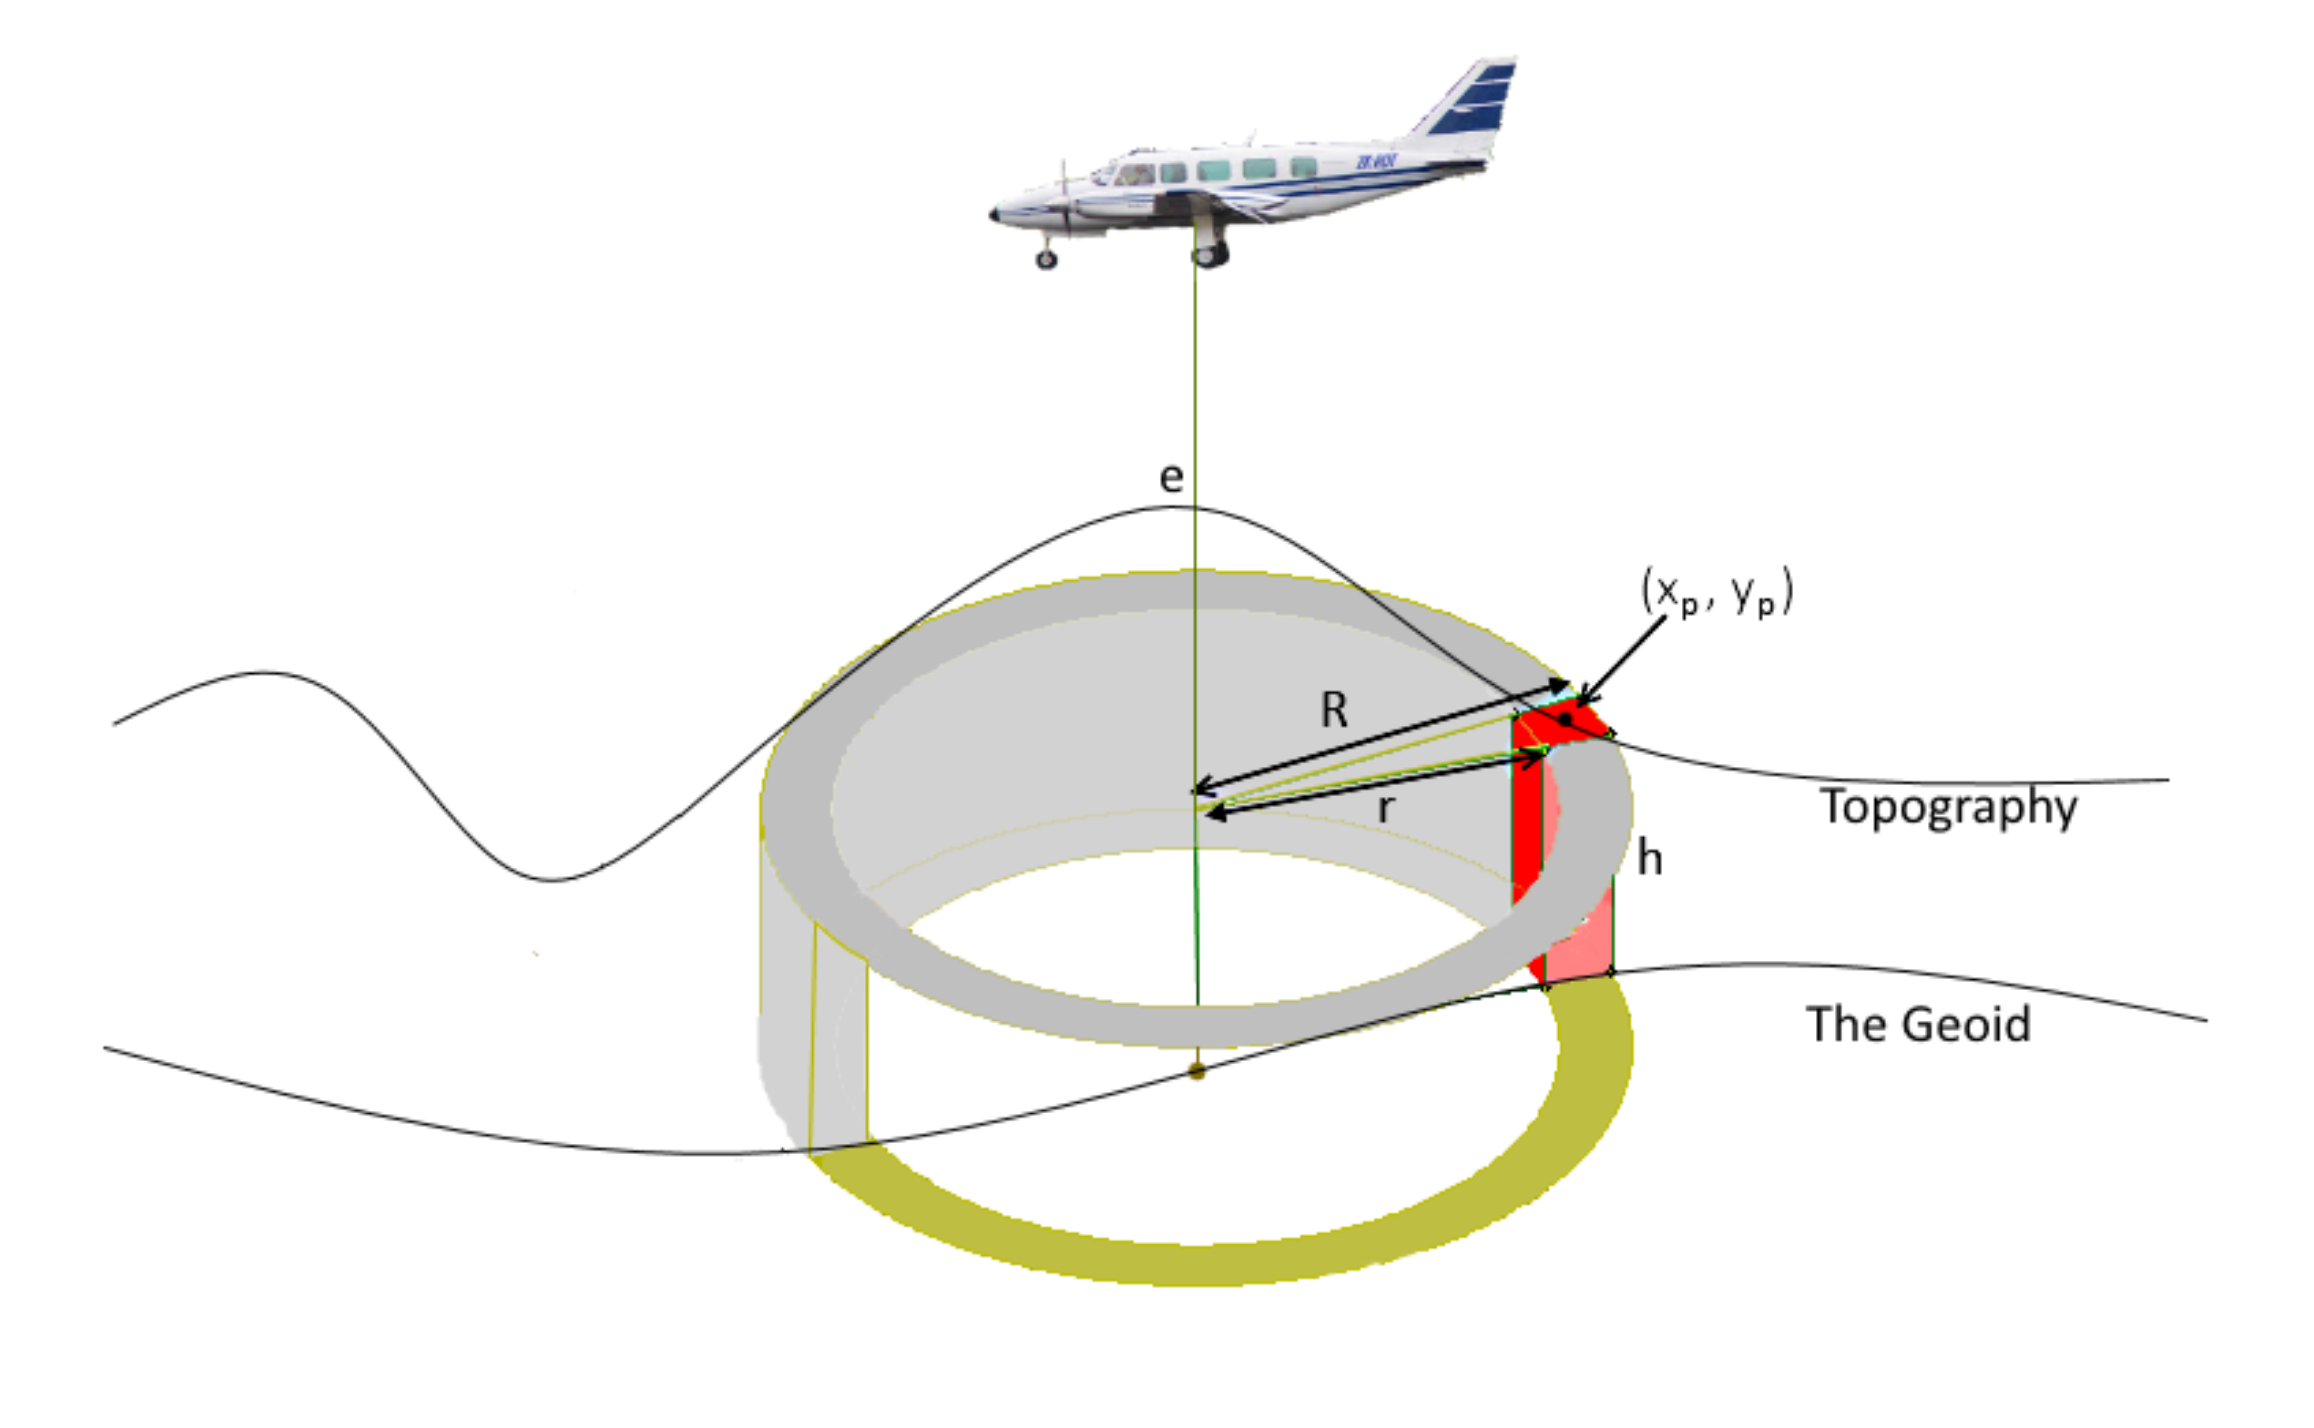
\includegraphics[width=0.7\linewidth]{figures/chp3/chp3_annulus.png}
  \caption[Annulus approximation of a vertical prism]{
    An illustration of an annulus of topography as an approximation for a vertical prism. From \citet{mccubbineairborne2016}.
  }
  \label{fig:chp3_annulus}
\end{figure}

A vertical prism can be approximated as a sector of an annulus (a cylindrical shell), as in Figure \ref{fig:chp3_annulus}. This approximation greatly simplifies the calculation of the vertical derivative of the prisms' gravity. The vertical component of gravity of an entire annulus (grey hollow cylinder in Figure \ref{fig:chp3_annulus}) is defined by

\begin{equation} \label{eq:annulus_gravity}
\delta g = 2 \pi G \rho (R - r + \sqrt{r^2 + h^2} - \sqrt{R^2 + h^2)}
\end{equation}

\noindent
where $\rho$ is the density, $G$ is the gravitational constant, $r$ and $R$ are the inner and outer radii, respectively, and $h$ is the average height of the cylinder \citep{hammerterrain1939}. $r$, $R$, and $h$ are relative to the observation point, located in the centre bottom of the annulus. \citet{mccubbineairborne2016} provides an adaption of Equation \ref{eq:annulus_gravity} which isolates the gravity of just a portion of this annulus (red section in Figure~\ref{fig:chp3_annulus}). This is accomplished by adding an additional factor $f$, relating the area of the annulus to the area of a sector of it:

\begin{equation}
f = \frac{\alpha^2}{\pi(R^2 - r^2)}
\end{equation}

\noindent
where

\begin{equation}
r = \sqrt{x^2+y^2} - \sqrt{\frac{\alpha^2}{2}}
\end{equation}

\begin{equation}
R = \sqrt{x^2+y^2} + \sqrt{\frac{\alpha^2}{2}}
\end{equation}

\noindent
where $\alpha$ is the prism width, $x$, $y$, and $z$ are coordinates of the prism centre, relative to the observation point. This factor $f$ is then multiplied by Equation~\ref{eq:annulus_gravity} to give the vertical component of gravity for a section of an annulus, $\delta g_{annulus} = f \delta g$.

Taking the derivative of this with respect to h gives

\begin{equation} \label{eq:vertical_derivative_annulus}
\dfrac{\partial g}{\partial h} = 2 f \pi G \rho h ( 
    \dfrac{1}{\sqrt{r^2 + h^2}} - \dfrac{1}{\sqrt{R^2 + h^2}} ).
\end{equation}

While the approximation of a prism as a section of an annulus introduces some errors, the calculation is efficient and simple to implement.

\paragraph*{Finite differences approximation}

Another option to calculate the vertical derivative for the Jacobian matrix is with numerical differentiation. For this, a small prism is added above each existing prism, its forward gravity is calculated and the result is divided by the small prism's height. This approximates the vertical derivative of gravity at the surface of the prism, relative to the observation point. \\

Both methods adequately determine the Jacobian. The annulus method is a more simple calculation and is thus faster, but is likely less accurate and introduces singularities. These singularities occur if the prism is directly beneath the observation point, so that either the inner or outer radii are negative (Figure \ref{fig:chp3_annulus}). These singularities are resolved by shifting the observation point to a prism edge. Conversely, the finite differences method, while it is a numerical approximation, uses analytical solutions for calculating the forward gravity \citep{nagygravitational2000, fatiandoaterraprojectharmonica2023}, and thus is valid in the entire domain, with no singularities. This increased robustness makes the computation slower. Section \ref{chp3_annulus_vs_prisms} compares the effectiveness and computation time of both of these methods.

\subsubsection{Least-squares solver}

With the Jacobian matrix and the vector of gravity residuals, Equation \ref{eq:matrix_eq} can be solved to find the set of surface correction values that minimize the fit function. Here, the matrix equation $\mathbb{J} \vv{x} = \vv{r}$ is solved with an iterative damped least squares algorithm \citep[LSQR][]{paigelsqr1982}. The algorithm gives the minimum-norm solution, where for a set of solutions that each fit the data with the same accuracy, the solution with the minimum $||p||^2$ is chosen. LSQR accepts a damping parameter, which helps regularize the problem, preventing the solution from becoming too large. The choice of the damping value is important as it directly affects the inverted results. The optimal value can be chosen with a cross-validation routine following that of \citet{uiedafast2017}, as described below.

\subsubsection{Regularization} \label{chp3:regularization}

Regularization is a series of techniques used to help constrain ill-posed inversion problems \citep{asterparameter2018}. Most potential field inversions, due to their inherent non-uniqueness, are ill-posed, containing many solutions which equally satisfy the data. Here regularization is split into \textit{smallness} and \textit{smoothness}. \textit{Smallness} deals with adhering to \textit{a priori} constraints, i.e. having the inverted surface elevation match the previous bathymetry measurements (constraint points). \textit{Smoothness} helps to achieve realistic topographic results, without major jumps or excessively steep slopes. 

\paragraph*{Smoothness}
To achieve a form of smoothness regularization, damping is applied at each iteration to the solver of the matrix equation. One method to choose an optimal damping value is cross-validation of the input gravity data \citep{uiedafast2017}. An effective inversion should produce a topography that, when forward-modelled, accurately recreates observed gravity data that weren't included in the inversion. This idea is the basis of the cross-validation routine. The observed gravity data is split into two sets, a \textit{training} and a \textit{testing} set. For an individual damping value, the inversion is run using only the training set. The final inverted bathymetry is then forward-modelled onto the observation points of the testing set. The difference between the observed and forward gravity at these testing points is calculated. The root mean square (RMS) of the differences provides a metric for the effectiveness of the damping; this is referred to as the \textit{score}. This process is then repeated for a suite of damping values, and the value which produces the lowest score is used as the optimal damping value. In this inversion, the gravity data, whether they are airborne flight lines or scattered ground stations, are interpolated onto a regular grid (see Section \ref{chp3:eq source resampled}). To create the testing set of observed gravity data, the original data are interpolated onto a grid at half the desired grid spacing. This leaves the training set with the desired number of points. This grid spacing configuration is shown in Figure \ref{fig:chp3_CV_grid_spacing}.

\begin{figure}[!ht]
    \centering
    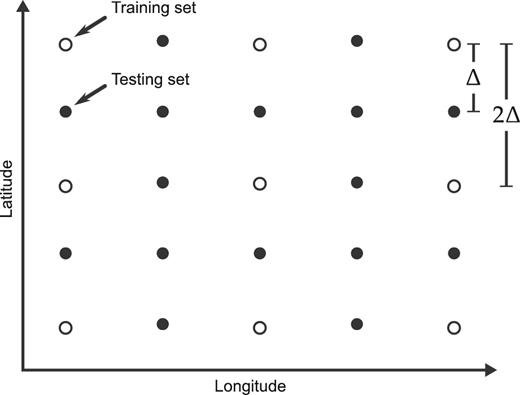
\includegraphics[width=0.5\textwidth]{figures/chp3/chp3_CV_grid_spacing.jpg}
    \caption[Training and testing set configuration]{Configuration of observed gravity data observation points, split into training and testing sets. Reprinted from \citet{uiedafast2017}.}
    \label{fig:chp3_CV_grid_spacing}
\end{figure}

\paragraph*{Smallness}
A form of smallness regularization is applied here to ensure the inversion results adhere to any \textit{a priori} bathymetry constraints. A portion of this smallness regularization is already accounted for when using the constraint point minimization method of regional-residual separation. This method minimizes the residual component of the gravity misfit at the constraint points by assigning the majority of the misfit to the regional component. However, non-zero residual values near the constraints will result in a non-zero correction of the prisms immediately surrounding the constraint. For further smallness regularization, a weighting grid (Figure \ref{fig:chp3_simple_weights}) is used to ensure the surface correction values at each iteration are 0 at constraint points. If only the prism immediately at the constraint point is fixed, a \textit{pedestal} effect commonly develops. This is where the nearby prisms' surfaces freely move during the inversion, yet the constrained prism is fixed, resulting in either a pedestal or a hole. To avoid this, the weighting grid smoothly decays from a value of 0 at the constraints, to a value of 1 at a distance. To create this grid, the minimum distance between each grid cell (prism) and the nearest constraint point is calculated. These values are then normalized from 0 to 1 (Figure \ref{fig:chp3_simple_weights}). At each iteration, the least squares solver yields a grid of surface correction values. Before being added to the prism layer, the grid is multiplied by this weighting grid. This results in surface corrections of 0 for prisms located at constraint points, unmodified surface correction values far from constraint points, and a smooth taper between these two endmembers. \\

\begin{figure}[!ht]
    \centering
    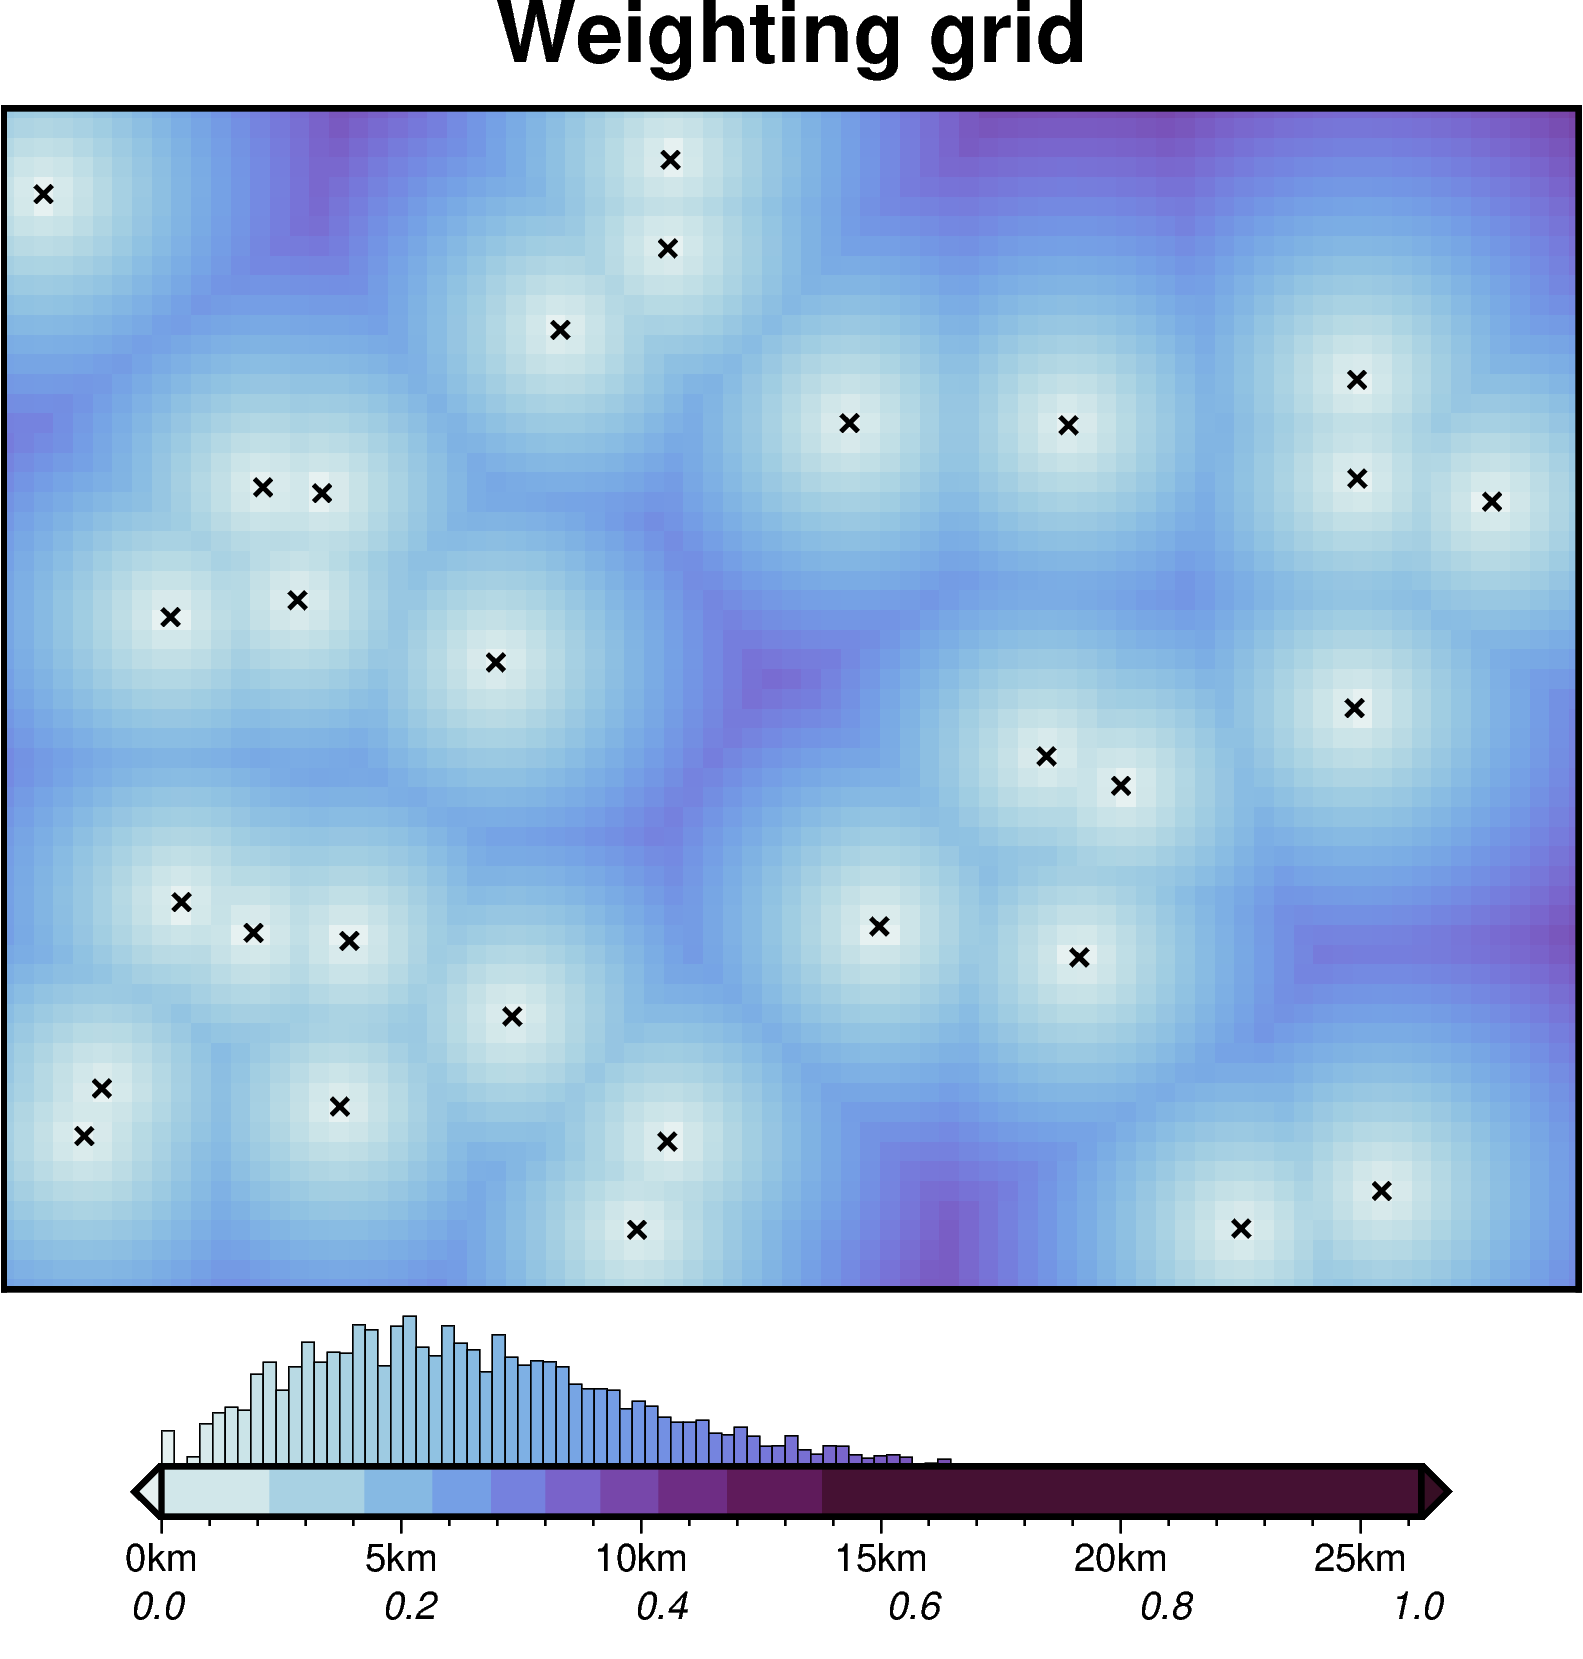
\includegraphics[width=0.5\textwidth]{chp3/chp3_simple_weights}
    \caption[Weighting grid for the simple synthetic inversion]{Weighting grid for the simple synthetic inversion, created from the minimum distance between each grid cell and the nearest constraint (black crosses). Grid values are normalized from 0 to 1 to produce the weighting grid (lower colourmap annotations).}
    \label{fig:chp3_simple_weights}
\end{figure}

The above sections outline a single iteration of the inversion. Once the surface correction is calculated and the weights are applied, these values are added to the starting bathymetry (or the last iterations inverted bathymetry). This is then re-discretized into prisms. The updated prisms are then forward modelled to create a new predicted gravity, $\vv{d}^{pred}$. This is subtracted from the observed gravity, $\vv{d}^{pred}$, to get a new misfit, $\vv{m}$. Using the same original regional component, the updated residual gravity misfit, $\vv{m}_{res}$, is calculated. This is now the input into the second iteration of the inversion. This process is repeated until a user-determined termination. Next, we outline the four criteria for ending the inversion. 

\subsection{Stopping Criteria} \label{chp3:stopping_criteria}

The inversion is terminated on one of four stopping criteria:

\begin{enumerate}
    \item when the inversion reaches a maximum number of iterations ($N$)
    \item when the $\ell^2$-norm of the residual ($||\vv{m}||_2$, Equation \ref{eq:misfit}) is less then a set $\ell^2$-norm tolerance
    \item if there is no significant variation in the $\ell^2$-norm between iterations (i.e. the $\Delta||\vv{m}||_2$ is less than a set tolerance)
    \item if the $\ell^2$-norm increases above a certain threshold of the starting $\ell^2$-norm. 
\end{enumerate}
The maximum number of iterations is set as a safety margin to avoid excessively long-running inversions. The $\ell^2$-norm tolerance is used to end the inversion before excessive over-fitting of noise in the data. This should be set to the square root of the assumed noise level of the gravity data. The $\Delta\ell$2-norm tolerance is used to end inversions that have reached their limit of reducing the $\ell^2$-norm, Finally, the upper limit of $\ell^2$-norm terminates run-away inversions, which occurred during the development of the inversion due to coding errors but is retained here as a fail-safe. 

\subsection{Software implementation}

The inversion algorithm described here is implemented within the Python programming language. The algorithm uses many open-source scientific libraries. These include Harmonica for the forward gravity modelling of prisms and equivalent sources calculations \citep{fatiandoaterraprojectharmonica2023, solergradientboosted2021}, Verde for various spatial operations \citep{uiedaverde2018}, PyGMT and Antarctic-Plots for figure creation \citep{uiedapygmt2021, tankersleyantarctic2023}, Scipy for least squares regression \citep{2020SciPy-NMeth}, and Optuna for hyperparameter optimization \citep{akibaoptuna2019}. The majority of the experiments were run in Jupyter notebooks \citep{pérezipython2007}, which are documented to explain the details of using the software. All source code, results, and figures involved in this chapter are made available in an online GitHub repository (\url{https://github.com/mdtanker/RIS_gravity_inversion}). See Section \ref{chp1_open_source} for the hardware used in this study.

\section{Synthetic models}
To assess the performance of the inversion and showcase its use, it is applied to a suite of synthetic test models. Each model has three components; 1) the `true' bathymetry surface, which the inversion is expected to model, 2) the `observed' gravity data, and 3) the `starting' bathymetry model, which is a low-resolution version of the true surface. The only inputs into the inversions are the observed gravity data and the starting bathymetry. The true bathymetry is only used to evaluate the performance of each inversion. The observed gravity data contains the forward gravity calculated from the true bathymetry, plus, in some cases, additional noise and other gravity signals such as a regional field. The starting bathymetry is created by sampling the true bathymetry at a set of points. These values are then used to re-grid the data for the entire region using a bi-harmonic spline interpolator \citep{uiedaverde2018}. This simulates the bathymetric knowledge of many ice shelves, where few direct measurements of bathymetry exist, such as drill holes, or single-point seismic surveys. These points are referred to as the constraints. The models tested here include:
\begin{enumerate}
    \item A simple model (Section \ref{chp3:simple_model}): This model sets a baseline performance expectation of the inversion, with no noise, dense gravity observation points, and no additional components included in the observed gravity. The synthetic bathymetry is created with Gaussian functions of various amplitudes and wavelengths. With this same simple model, the observed gravity data is re-gridded at a lower resolution, and random noise is added, to better simulate a gravity survey.
    \item A simple model with a regional field (Section \ref{chp3:simple_regional_model}): Using the same model as above, a `regional' component of the gravity field is added to the observed data.
    \item A semi-realistic model (Section \ref{chp3:Ross_Sea}): This last model is created from real bathymetry data from Antarctica's Ross Sea. This model tests the inversion's capabilities with more realistic bathymetric features expected for sub-ice-shelf environments.
\end{enumerate} 

\subsection{Simple model}\label{chp3:simple_model}

 \begin{figure}[!ht]
    \centering
    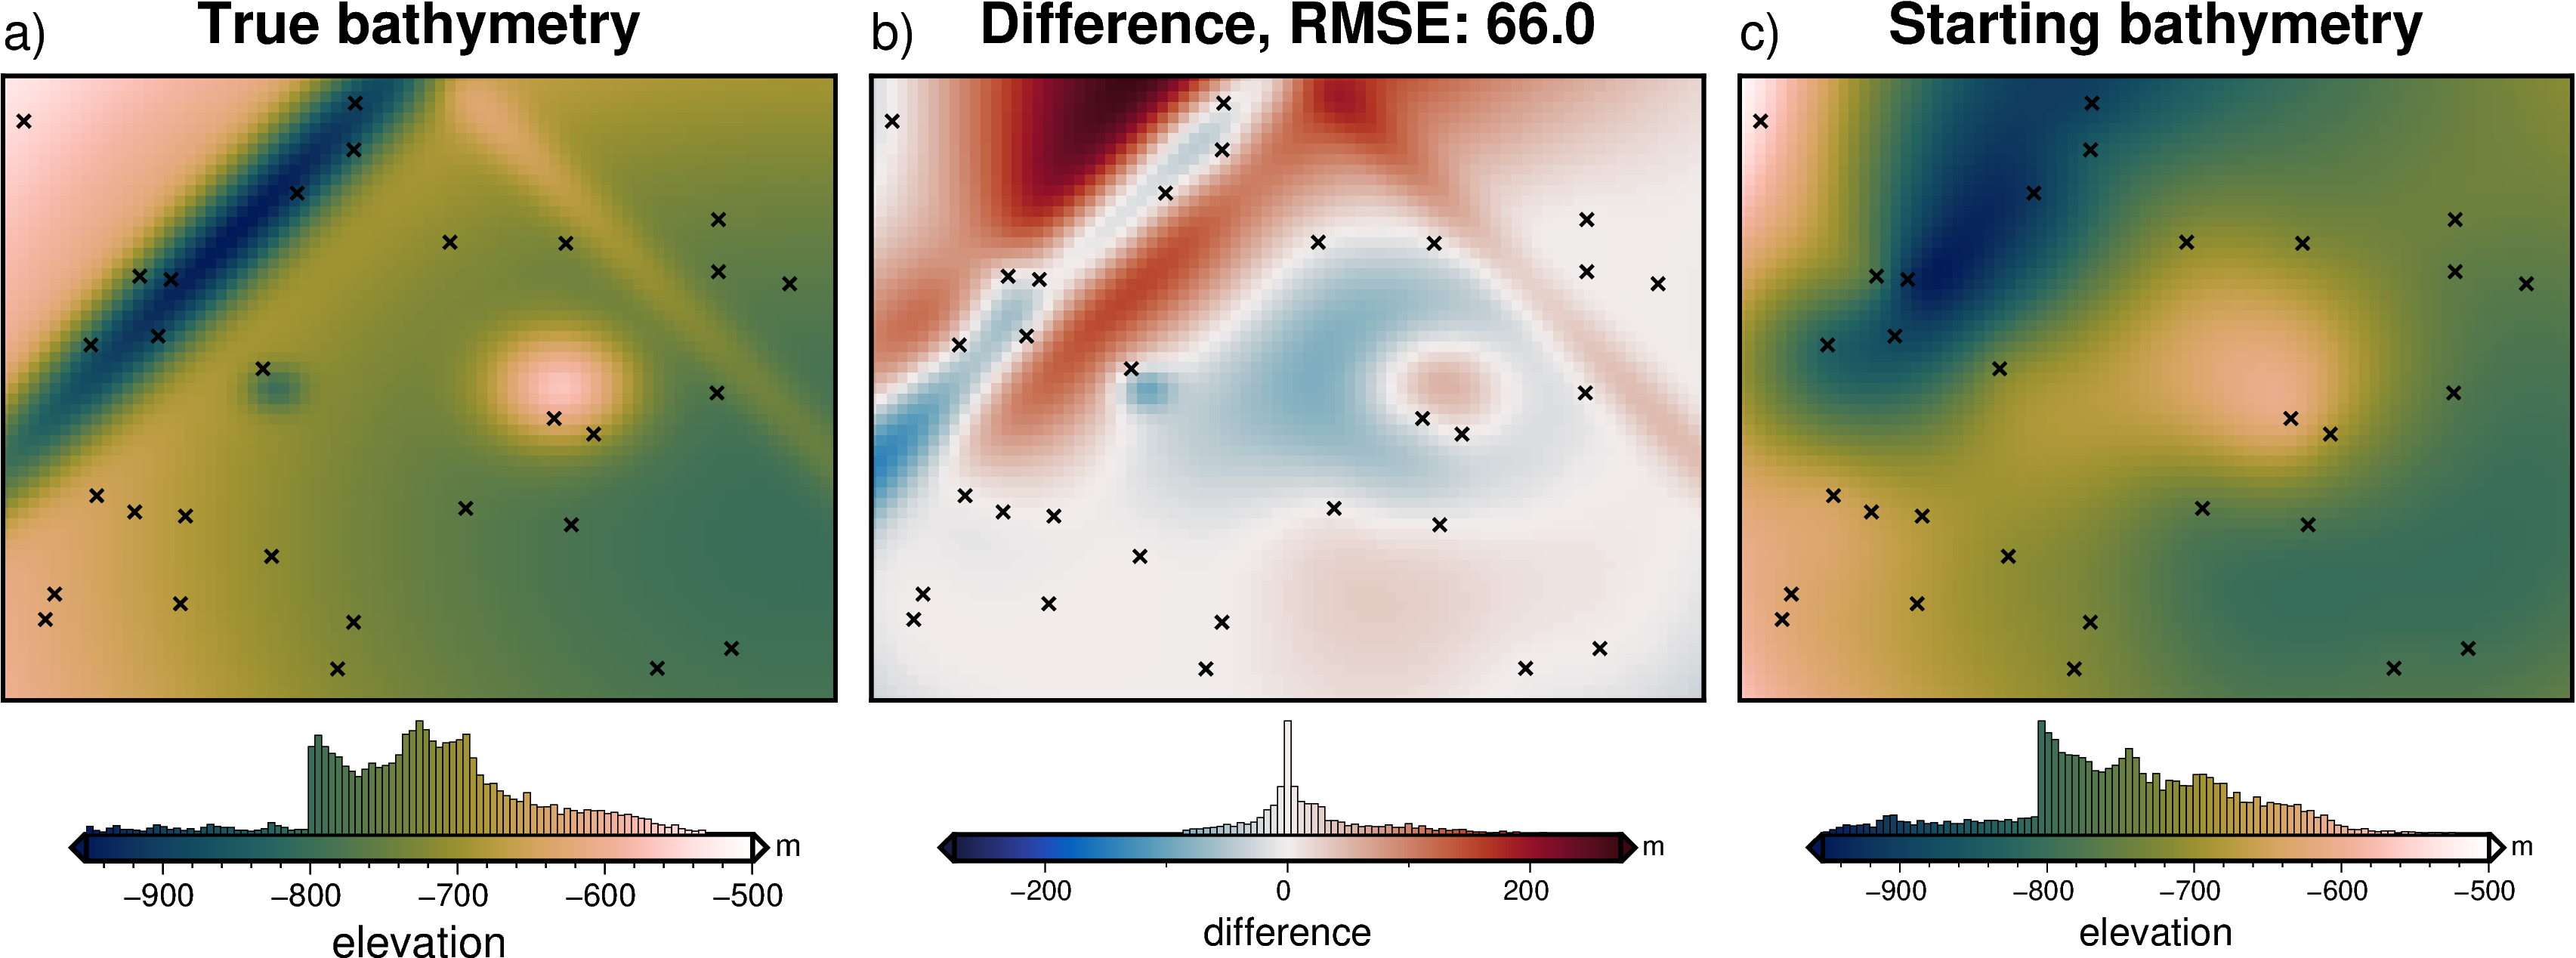
\includegraphics[width=0.95\textwidth]{chp3/chp3_simple_starting_model}
    \caption[Simple synthetic model bathymetry]{Simple synthetic model bathymetry. \textbf{a)} True bathymetry created from Gaussian functions, \textbf{b)} difference between a and c, and \textbf{c)} starting bathymetry, created from the sampling and re-gridding of the true bathymetry at 30 points (black crosses).}
    \label{fig:chp3_simple_starting_model}
\end{figure}

\subsubsection{Model setup}
Simulating typical sub-ice-shelf bathymetry, this model (Figure \ref{fig:chp3_simple_starting_model}a) has an average elevation of $\sim$ -700~m and ranges between $\sim$ -400~m and $\sim$ -1000~m. It contains features of various wavelengths, amplitudes, and shapes; namely two circular features and two linear features. Overall, the grid is eastward deepening and contains a shallow and wide E-W trough through the centre. The model domain is 80~x~60~km, with 1~km grid cells (4800 cells). A 6~km buffer zone in all directions was included to limit gravitational edge effects. 30 randomly located constraint points were used to create the starting bathymetry (Figure \ref{fig:chp3_simple_starting_model}c). The starting bathymetry has an RMS difference with the true bathymetry of 66~m. \\

To forward model the gravity of the true bathymetry, a layer of adjacent vertical right-rectangular prisms was created using the reference discretization method (Figure \ref{fig:chp3_discretization}e) with the mean elevation as the reference level. A density contrast of $\Delta\rho$ = 1276~kg~m\textsuperscript{-1} (contrast between seawater(1024~k~ m\textsuperscript{-1}) and sediment (2300~kg~m\textsuperscript{-1})), was used, with $+\Delta\rho$ for prisms above the reference, and $-\Delta\rho$ for prisms below the reference. The forward gravity of this prism layer was calculated at a constant height of 1000~m (roughly 1700~m above the bathymetry) on a regular grid at half the grid spacing (500~m) of the bathymetry. This represents the observed gravity data (Figure \ref{fig:chp3_simple_misfit}a) and consists of both the training and testing data sets used for the cross-validation (Section \ref{chp3:regularization}, Figure \ref{fig:chp3_CV_grid_spacing}). \\

The low-resolution starting layer was discretized in the same method, and the same density contrast was used. The forward gravity of these starting layer prisms results in the predicted gravity (Figure \ref{fig:chp3_simple_misfit}c). To account for any offset between the observed and predicted data, the observed data is DC-shifted to minimize the differences at the constraint points. The difference between the shifted observed and the predicted data gives the gravity misfit (Figure \ref{fig:chp3_simple_misfit}b). Since there is no regional component in this synthetic model, the input into the inversion, the residual misfit, is equal to this total misfit (Equation \ref{eq:regional_residual}). This residual misfit describes the ability of the starting model to predict the observed data. 

\begin{figure}[!ht]
    \centering
    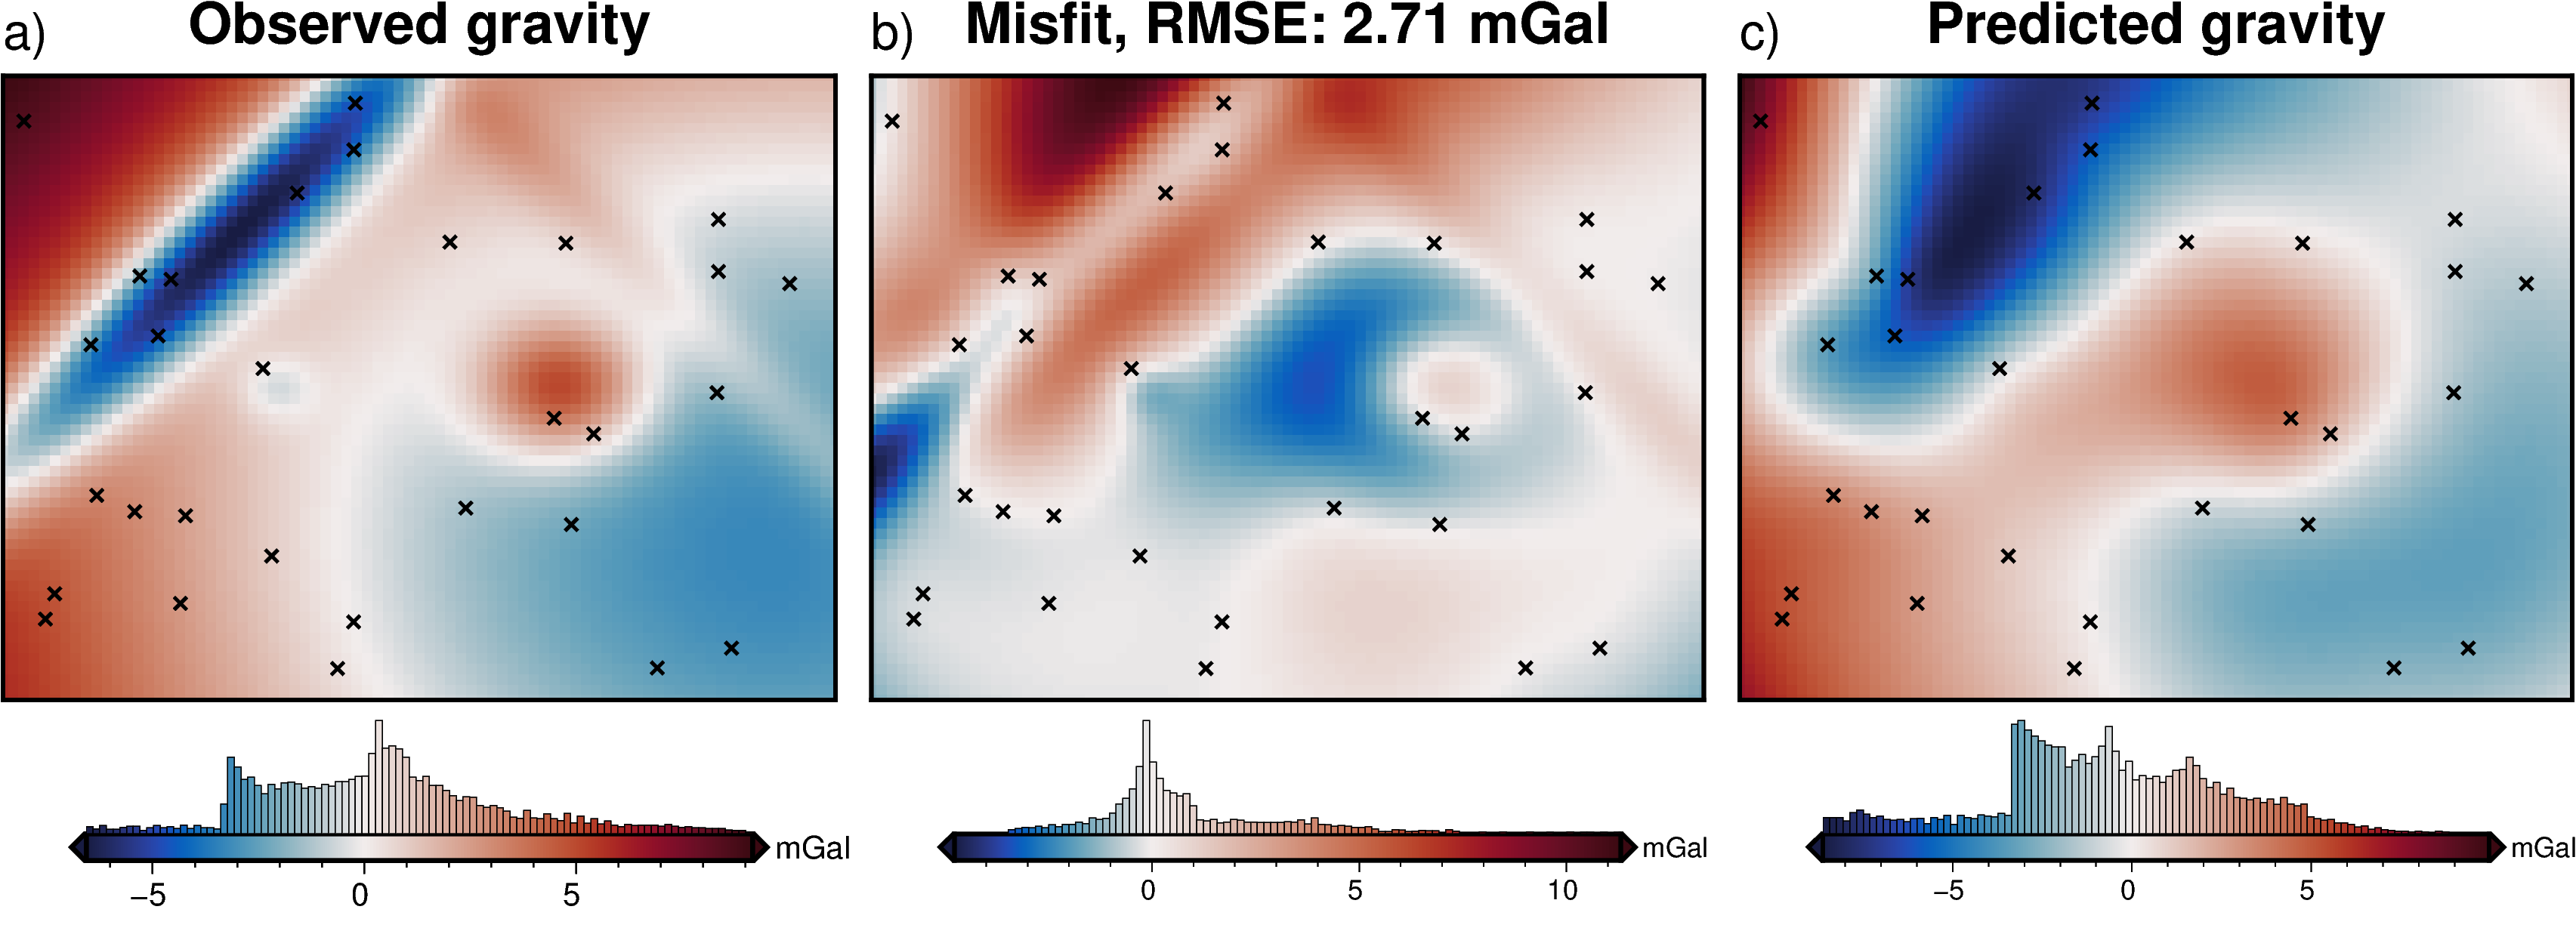
\includegraphics[width=0.95\textwidth]{chp3/chp3_simple_misfit}
    \caption[Simple synthetic gravity anomalies]{\textbf{a)} Synthetic gravity data generated from the true bathymetry, \textbf{b)} the residual anomaly, defined as the difference between a and c, and \textbf{c)} the predicted gravity from the starting bathymetry (Figure \ref{fig:chp3_simple_starting_model}c).}
    \label{fig:chp3_simple_misfit}
\end{figure}

\subsubsection{Cross validation} \label{chp3:simple_model_CV}
To find the optimal value for the regularization damping parameter, the cross-validation method of \citet{uiedafast2017} is used (Section \ref{chp3:regularization}). The full set of observed data with a 500~m spacing ($N$~=~19481), was separated into the training ($N$~=~4941) and testing set ($N$~=~14540). With the grid configuration from Figure \ref{fig:chp3_CV_grid_spacing}, the resulting training data was on a regular 1~km grid, which matches the grid of the bathymetry. This training data set was used as the input to 10 inversions. Each inversion used a different damping value between 10\textsuperscript{-4} and 10\textsuperscript{-1}. The resulting inverted bathymetry of each inversion was then forward-modelled on the observation points of the testing data set (not used in the inversion). The RMS difference between the forward-modelled gravity value and the initial residual misfit values was calculated, giving the cross-validation score (Figure \ref{fig:chp3_simple_CV_and_profile}a). Of the 10 inverted bathymetry models, the model with the lowest score is retained.

\begin{figure}[!ht]
    \centering
    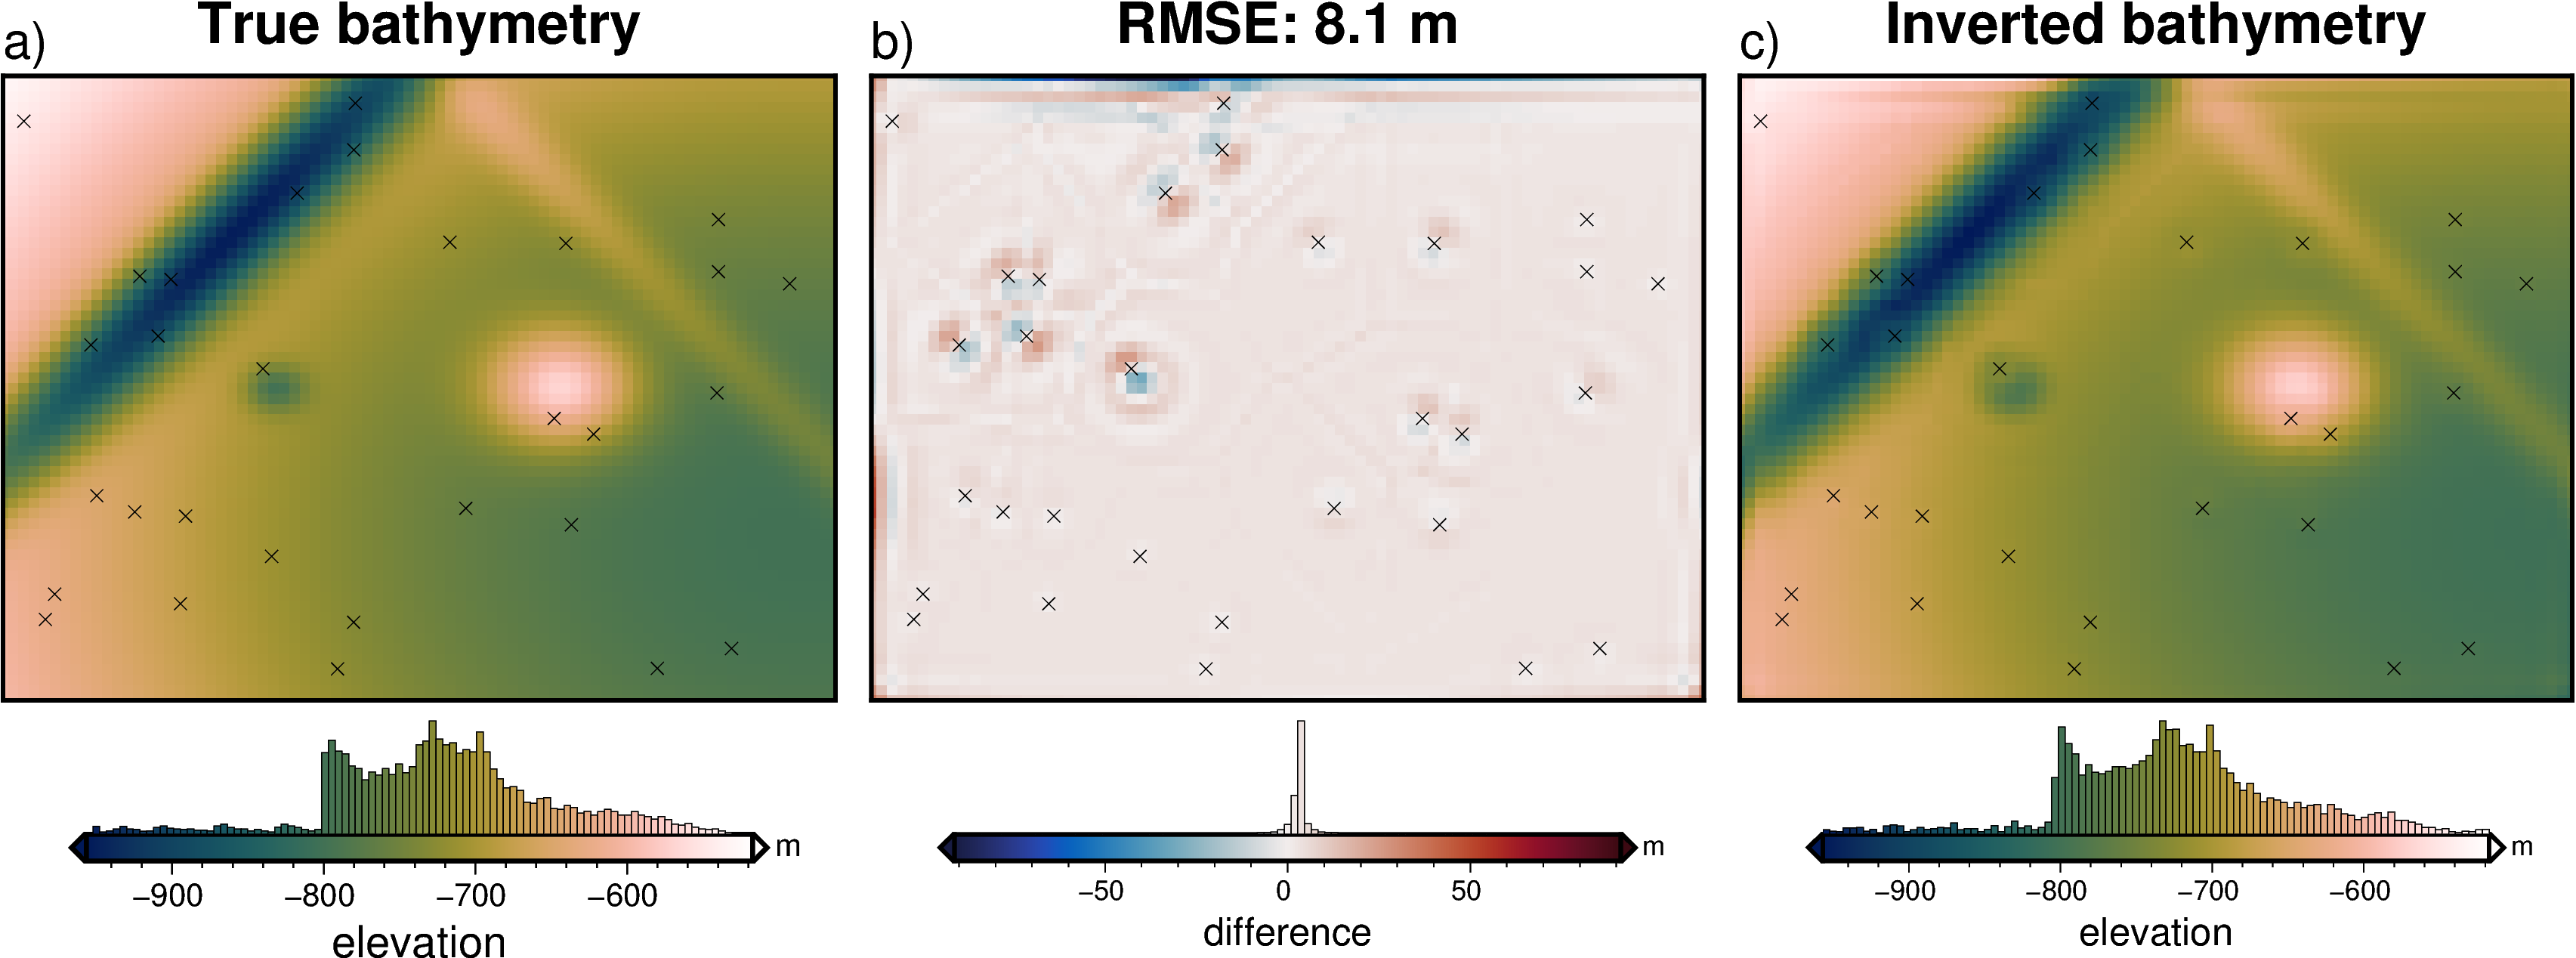
\includegraphics[width=.95\textwidth]{figures/chp3/chp3_simple_results.png}
    \caption[Annulus approximation inversion results]{Inverted results with optimized parameters, using the annulus approximation method of calculating the Jacobian matrix. \textbf{a)} True bathymetry, \textbf{b)} difference between a and c, and \textbf{c)} final inverted bathymetry. Black crosses are constraint points. The RMS difference with the true bathymetry at these constraints is 1 m}
    \label{fig:chp3_simple_results}
\end{figure}

This model is shown in Figure \ref{fig:chp3_simple_results}c, and resulted from a damping value of 10\textsuperscript{-2}. This inverted bathymetry has an RMS difference with the true bathymetry of 8~m and an RMS difference at the constraint points of 1~m. Figure \ref{fig:chp3_simple_CV_and_profile}b shows a profile across the model. The overlap of the true (red) and inverted (blue) bathymetry in the first panel shows the effectiveness of the inversion at recovering the true bathymetry. The lower panel shows the inversion's ability to minimize the misfit between the observed gravity (red) and the forward response of the inverted bathymetry (blue). The inversion was able to recover all the features of the true bathymetry, with only minor errors along the edges of the domain, and adjacent to constraint points. For this simple model, the inversion converged in 37 iterations, with a total computation time of 30~seconds and a final RMS residual misfit of 0.022~mGal. It terminated due to the $\ell^2$-norm decreasing between the set threshold of 0.15 (0.0225~mGal).

\begin{figure}[!ht]
  \centering
    \begin{subfigure}[t]{.40\textwidth}
        \centering
        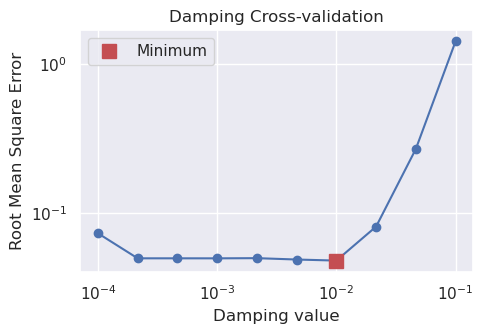
\includegraphics[width=\textwidth]{figures/chp3/chp3_simple_CV.png}
        \caption{}
    \end{subfigure}
    \begin{subfigure}[t]{.58\textwidth}
        \centering
        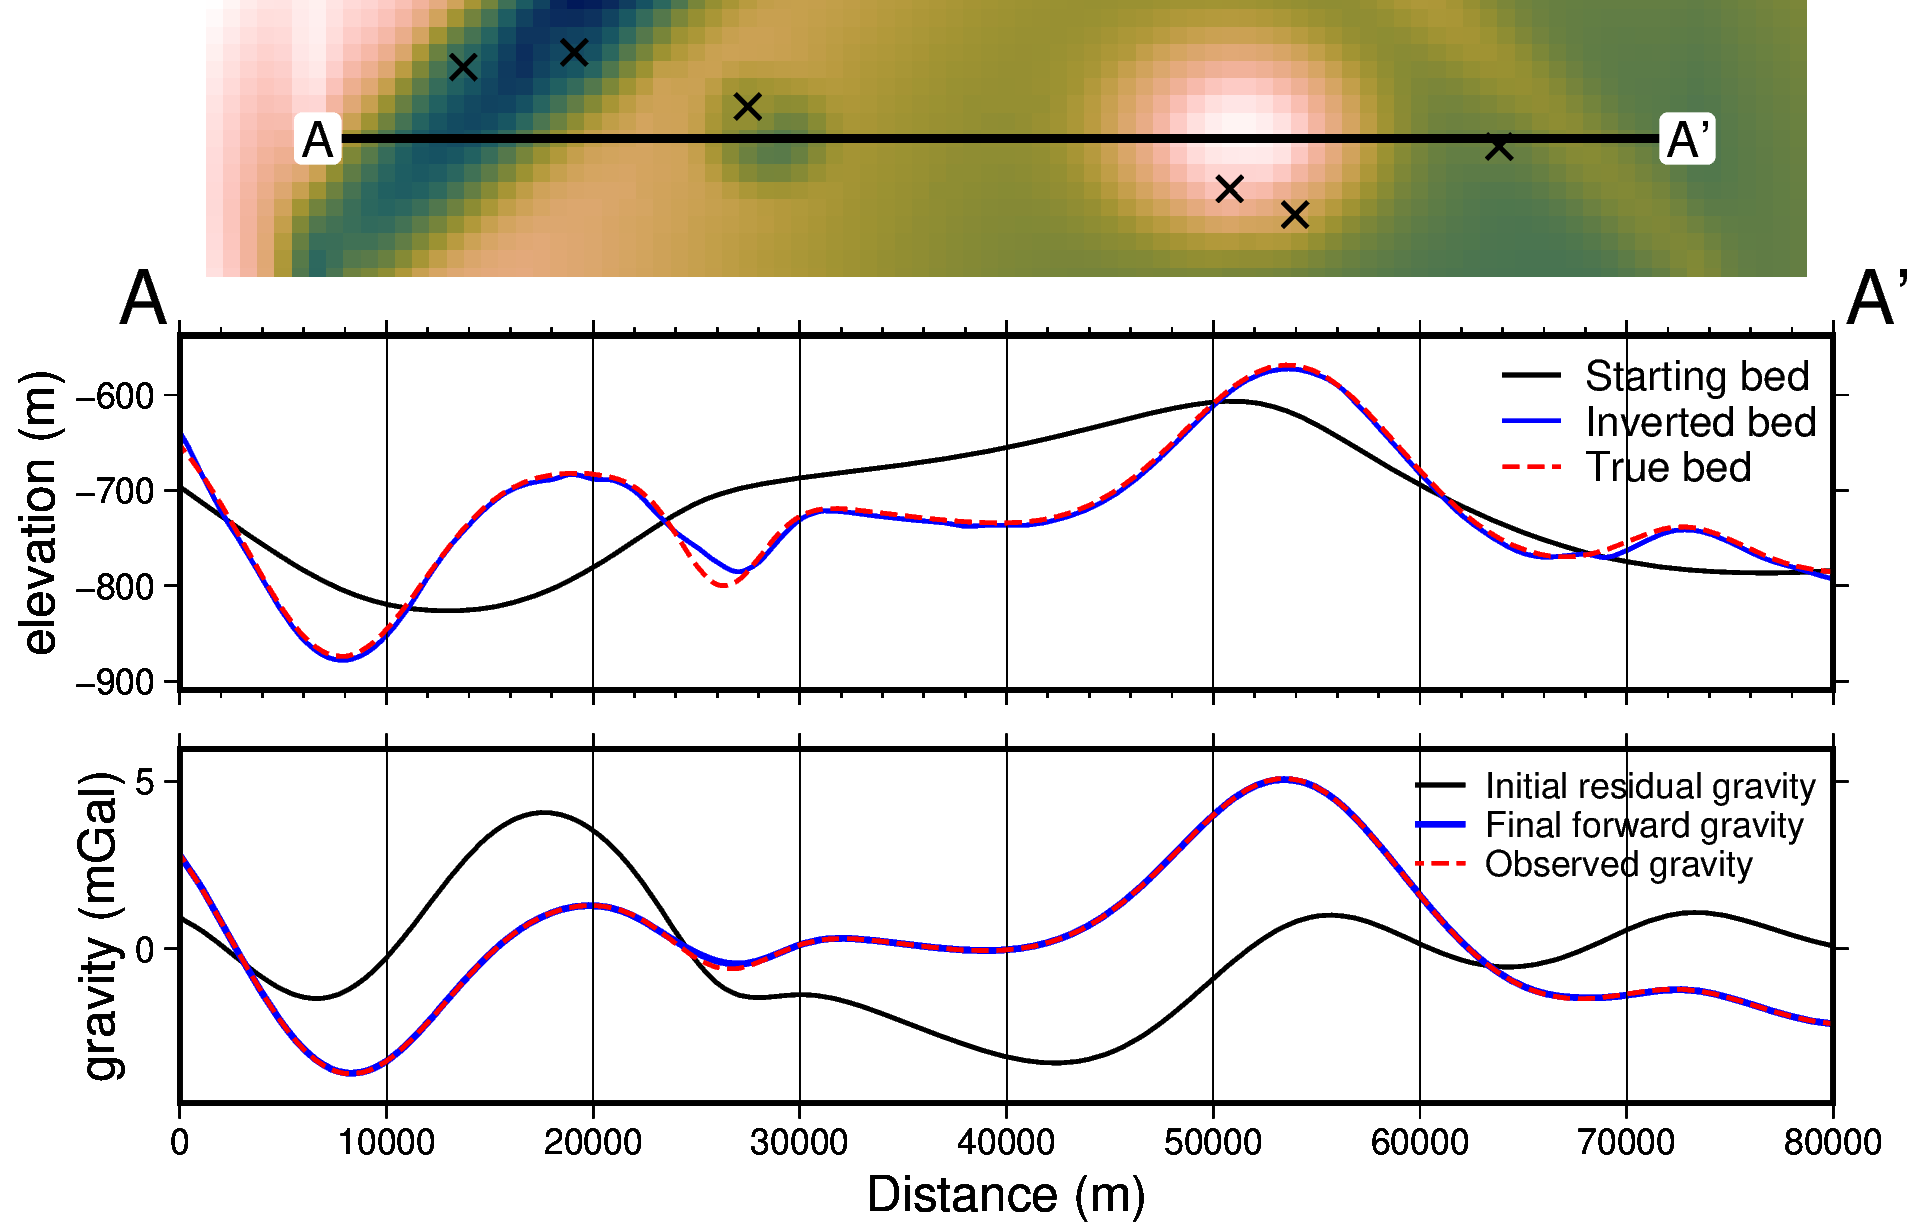
\includegraphics[width=\textwidth]{figures/chp3/chp3_simple_profile.png}
        \caption{}
    \end{subfigure}
  \caption[Annulus approximation inversion cross-validation and profile]{Cross-validation and profiles for the simple synthetic inversion. \textbf{a)} Cross-validation curve showing the optimal damping parameter (red square). Both axes are on a logarithmic scale. \textbf{b)} 2D profile of the inversion results. The top panel shows profile location and constraint points (black crosses). The middle panel contains topographic profiles of the starting, inverted, and true bathymetries. The bottom panel contains gravity anomaly profiles.}
    \label{fig:chp3_simple_CV_and_profile}
\end{figure}

\subsubsection{Comparing vertical derivative methods} \label{chp3_annulus_vs_prisms}
Section \ref{chp3:jacobian_methods} presented two methods for calculating the vertical derivative of gravity of a prism. This vertical derivative is used to create the Jacobian matrix (Equation \ref{eq:matrix_eq}) and needs to be calculated at each iteration of the inversion. The above cross-validation and inversion were performed using the \textit{annulus approximation} of the vertical derivative. Here, this process is repeated with the \textit{finite differences} method of the vertical derivative. Figure \ref{fig:chp3_simple_prisms_approx_results}) shows the results of this inversion. The optimal damping parameter was 10\textsuperscript{-2}, and the inversion resulted in an RMS difference with the true bathymetry of 9~m, compared to 8~m for the annulus approximation. Figure \ref{fig:chp3_annulus_vs_prisms_convergence} shows the inversion convergence curves for the inversion of the annulus approximation and the finite differences methods. The inversion with the annulus approximation was $\sim$500\% faster to converge than the finite differences method (30~sec vs 169~sec). Because these vertical derivatives need to be recalculated at each iteration, a large portion of the inversion time is spent performing these calculations. This comparison shows the annulus approximation is not only significantly faster, but results in comparable, or slightly more accurate, inversion results. For the remainder of this chapter, only the annulus approximation will be used.

\begin{figure}[!ht]
    \centering
    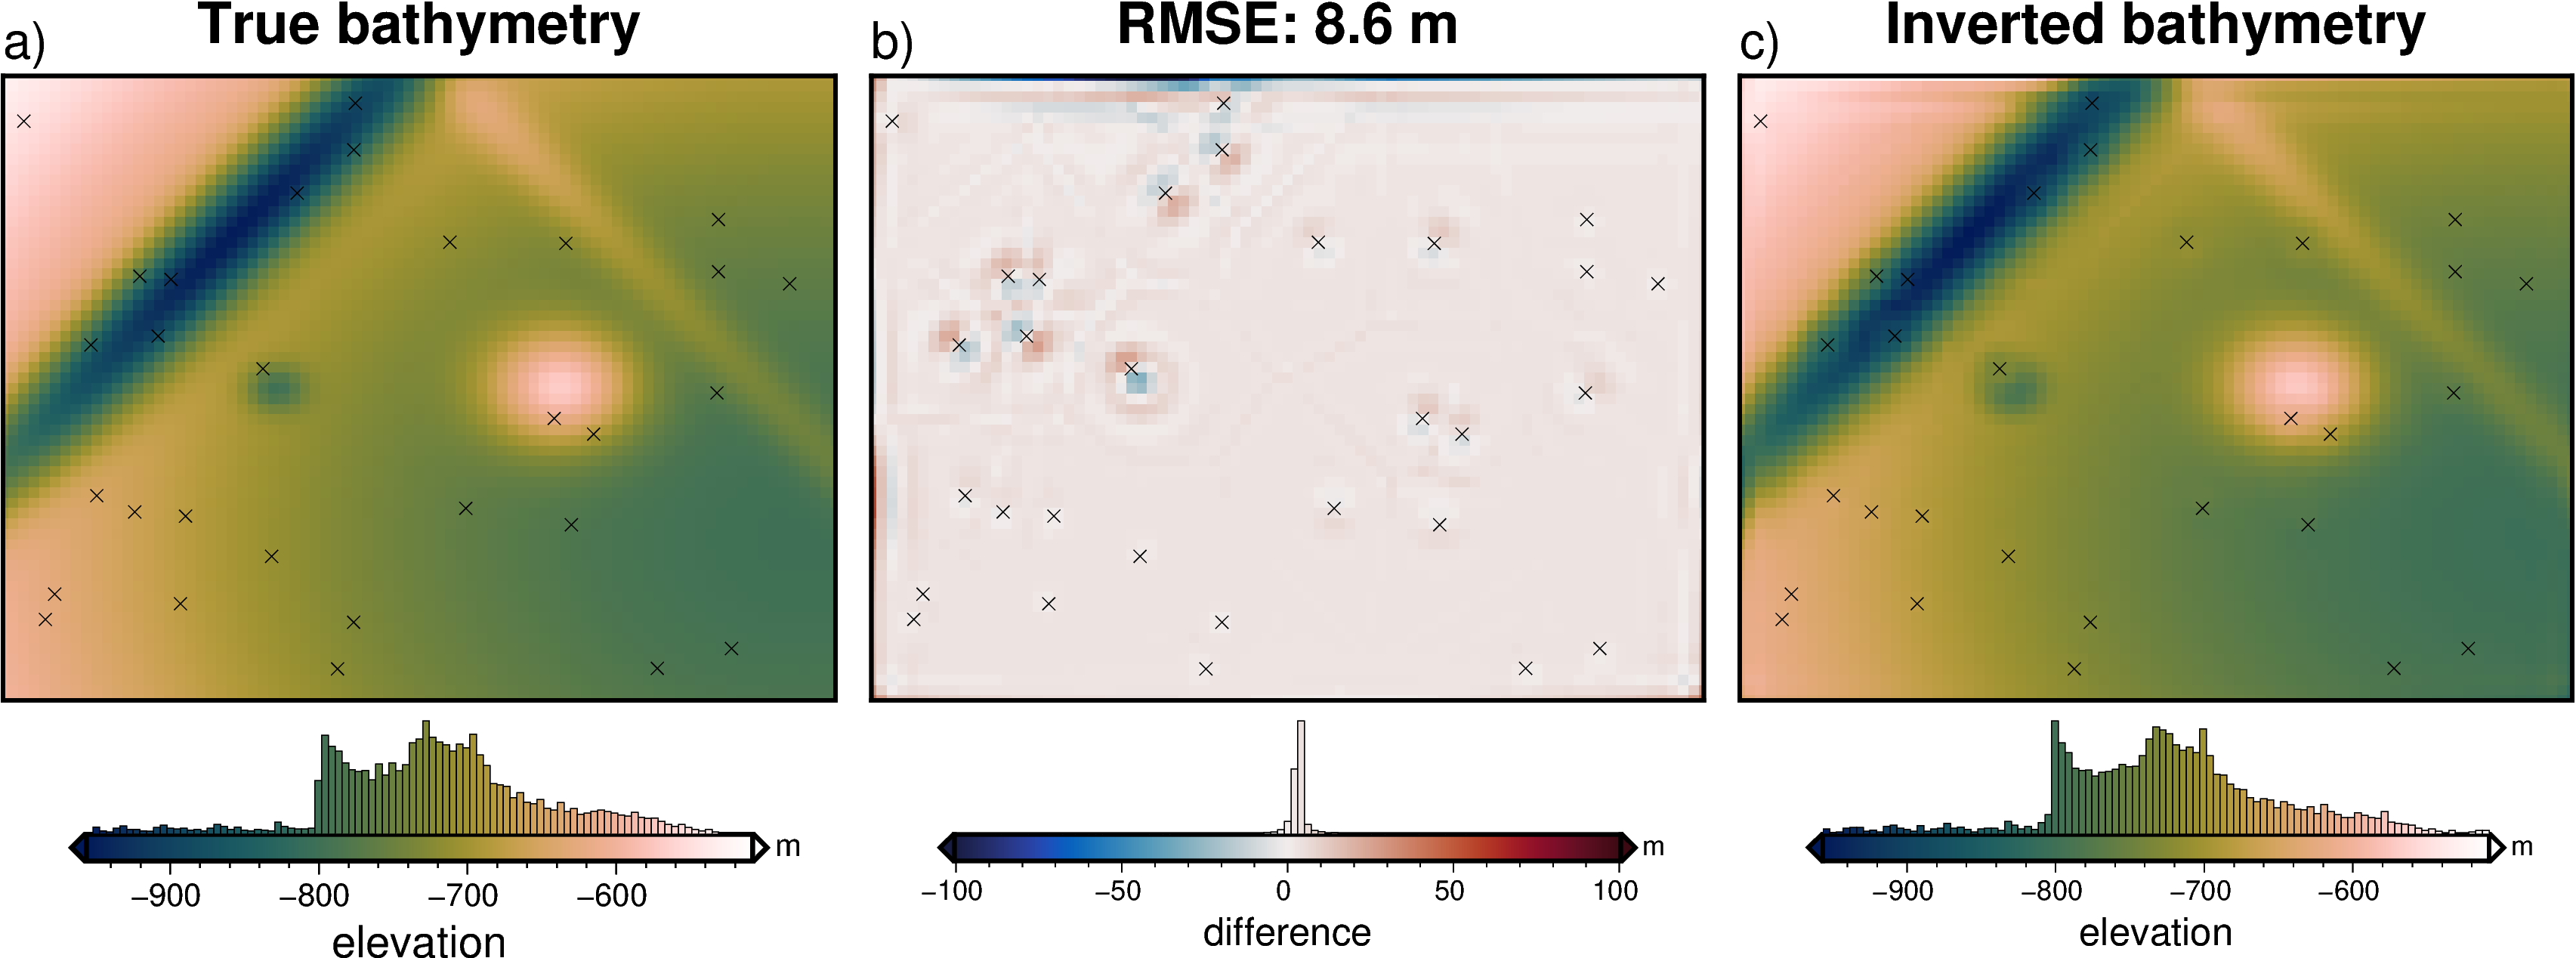
\includegraphics[width=.95\textwidth]{figures/chp3/chp3_simple_prisms_derivative_results.png}
    \caption[Finite differences inversion results]{Inversion results with optimized parameters using the finite differences method. \textbf{a)} True bathymetry, \textbf{b)} difference between a and c, and \textbf{c)} final inverted bathymetry. Black crosses are constraint points. The RMS difference with the true bathymetry at these constraints is 1~m}
    \label{fig:chp3_simple_prisms_approx_results}
\end{figure}

\begin{figure}[!ht]
  \centering
    \begin{subfigure}[t]{.48\textwidth}
        \centering
        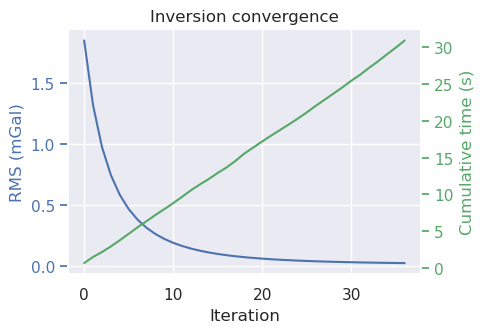
\includegraphics[width=\textwidth]{figures/chp3/chp3_simple_convergence.png}
        \caption{}
    \end{subfigure}
    \begin{subfigure}[t]{.48\textwidth}
        \centering
        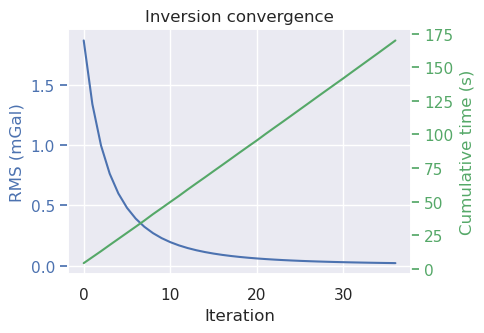
\includegraphics[width=\textwidth]{figures/chp3/chp3_simple_prisms_derivative_convergence.png}
        \caption{}
    \end{subfigure}
  \caption[Finite differences and annulus approximation convergence curves]{Inversion convergence curves for the two methods of creating the Jacobian matrix. Blue line (left y-axis) shows the RMS of the residual misfit at each iteration of the inversion. Green line (right y-axis) shows the cumulative time to complete the inversion. \textbf{a)} Results for the annulus approximation method of finding the vertical derivative. \textbf{b)} Results for the finite differences method.}
    \label{fig:chp3_annulus_vs_prisms_convergence}
\end{figure}

\subsubsection{Added noise}
To test the effect of noise in the gravity data, which is inevitable in data collection, especially so in airborne surveying, the observed gravity was contaminated with noise. The noise has a Gaussian distribution with a mean of 0~mGal and a standard deviation of 2\% of the max absolute value of the data ($\sim$ .16~mGal). Similarly, \citet{rashidifardconstraining2021} used 5\% noise in their synthetic gravity inversion while \citet{uiedafast2017} use 5~mGal of noise, which for their synthetic application equated to $\sim$~1\% of the max absolute value. Using this noise-corrupted gravity data, the same damping parameter cross-validation was run as previously (Figure \ref{fig:chp3_simple_noise_CV_and_profile}a), and the lowest score was achieved with a damping value of 10\textsuperscript{-2}. Figure \ref{fig:chp3_simple_noise_results} shows the inversion results of this noise-contaminated model. 
The inversion converged in 18 iterations, with a total computation time of 13 seconds and a final RMS residual misfit of 0.16~mGal. It terminated after the $\ell^2$-norm became lower than the set tolerance of 0.4 (0.16~mGal). This tolerance was set to match the known level of noise. The inverted bathymetry had an RMS difference of 12~m with the true bathymetry and an RMS difference of $<$~1~m at the constraint points. Figure \ref{fig:chp3_simple_noise_CV_and_profile}b shows the inversion is still able to reproduce the observed gravity (lower panel), but a component of the noise was introduced into the final bathymetry (upper panel). All major features of the true bathymetry are recovered, albeit not as accurately as the no-noise model (Figure \ref{fig:chp3_simple_results}).

\begin{figure}[!ht]
    \centering
    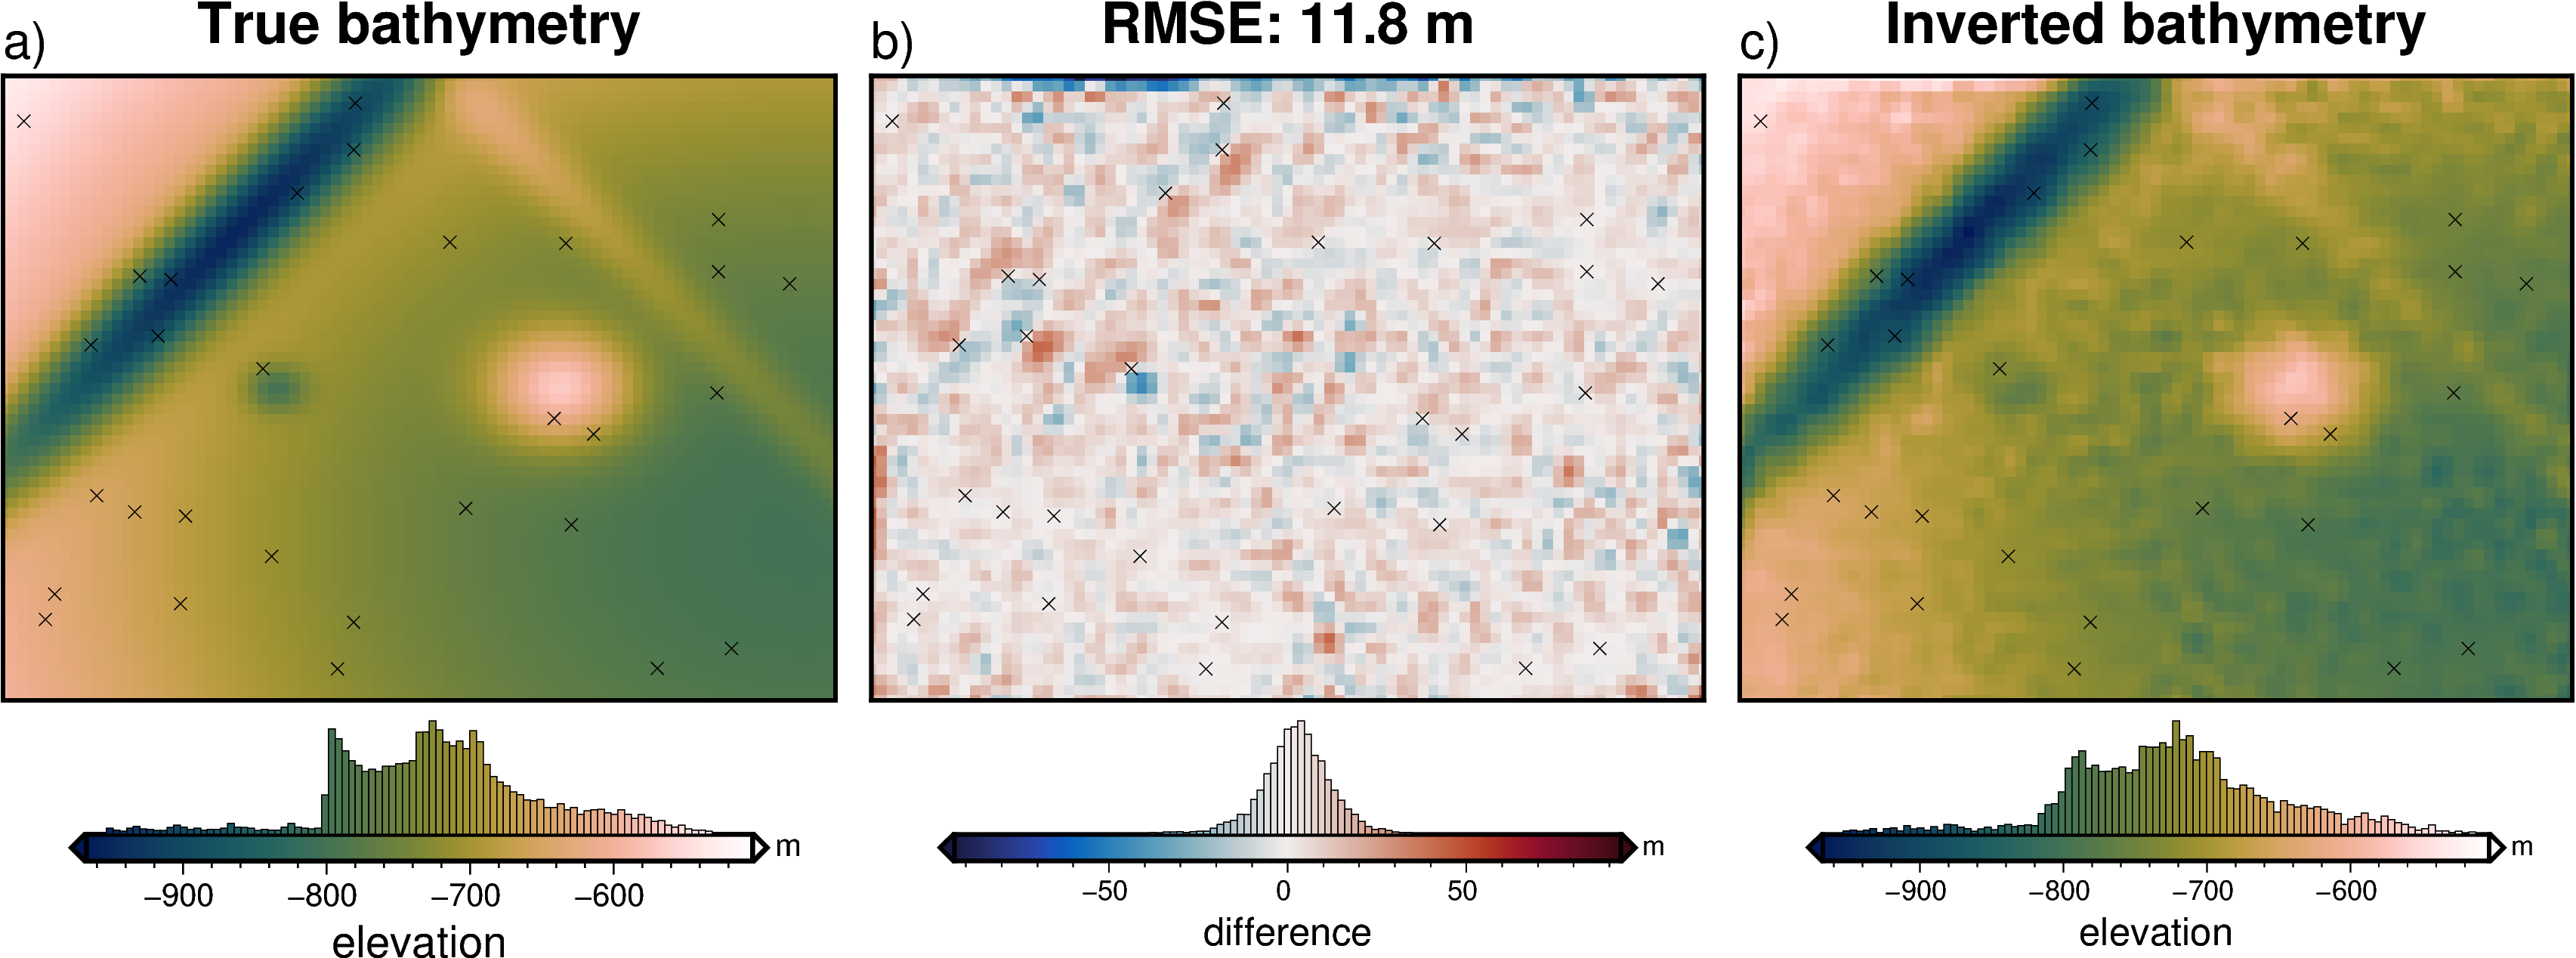
\includegraphics[width=0.95\textwidth]{chp3/chp3_simple_noise_results}
    \caption[Synthetic inversion with noise]{Simple synthetic model inversion results with 2\% added noise (0.16~mGal). \textbf{a)} True bathymetry, \textbf{b)} difference between a and c, \textbf{c)} final inverted bathymetry. Black crosses are constraint points. The RMS difference with the true bathymetry at these constraints is $<$~1~m.}
    \label{fig:chp3_simple_noise_results}
\end{figure}

\begin{figure}[!ht]
  \centering
    \begin{subfigure}[t]{.40\textwidth}
        \centering
        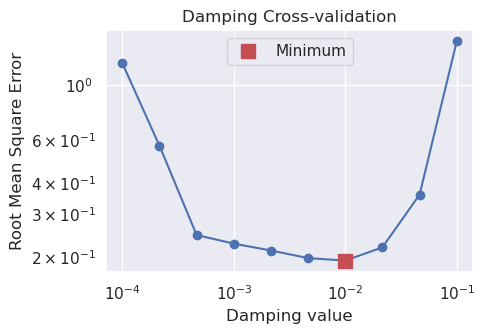
\includegraphics[width=\textwidth]{figures/chp3/chp3_simple_noise_CV.png}
        \caption{}
    \end{subfigure}
    \begin{subfigure}[t]{.58\textwidth}
        \centering
        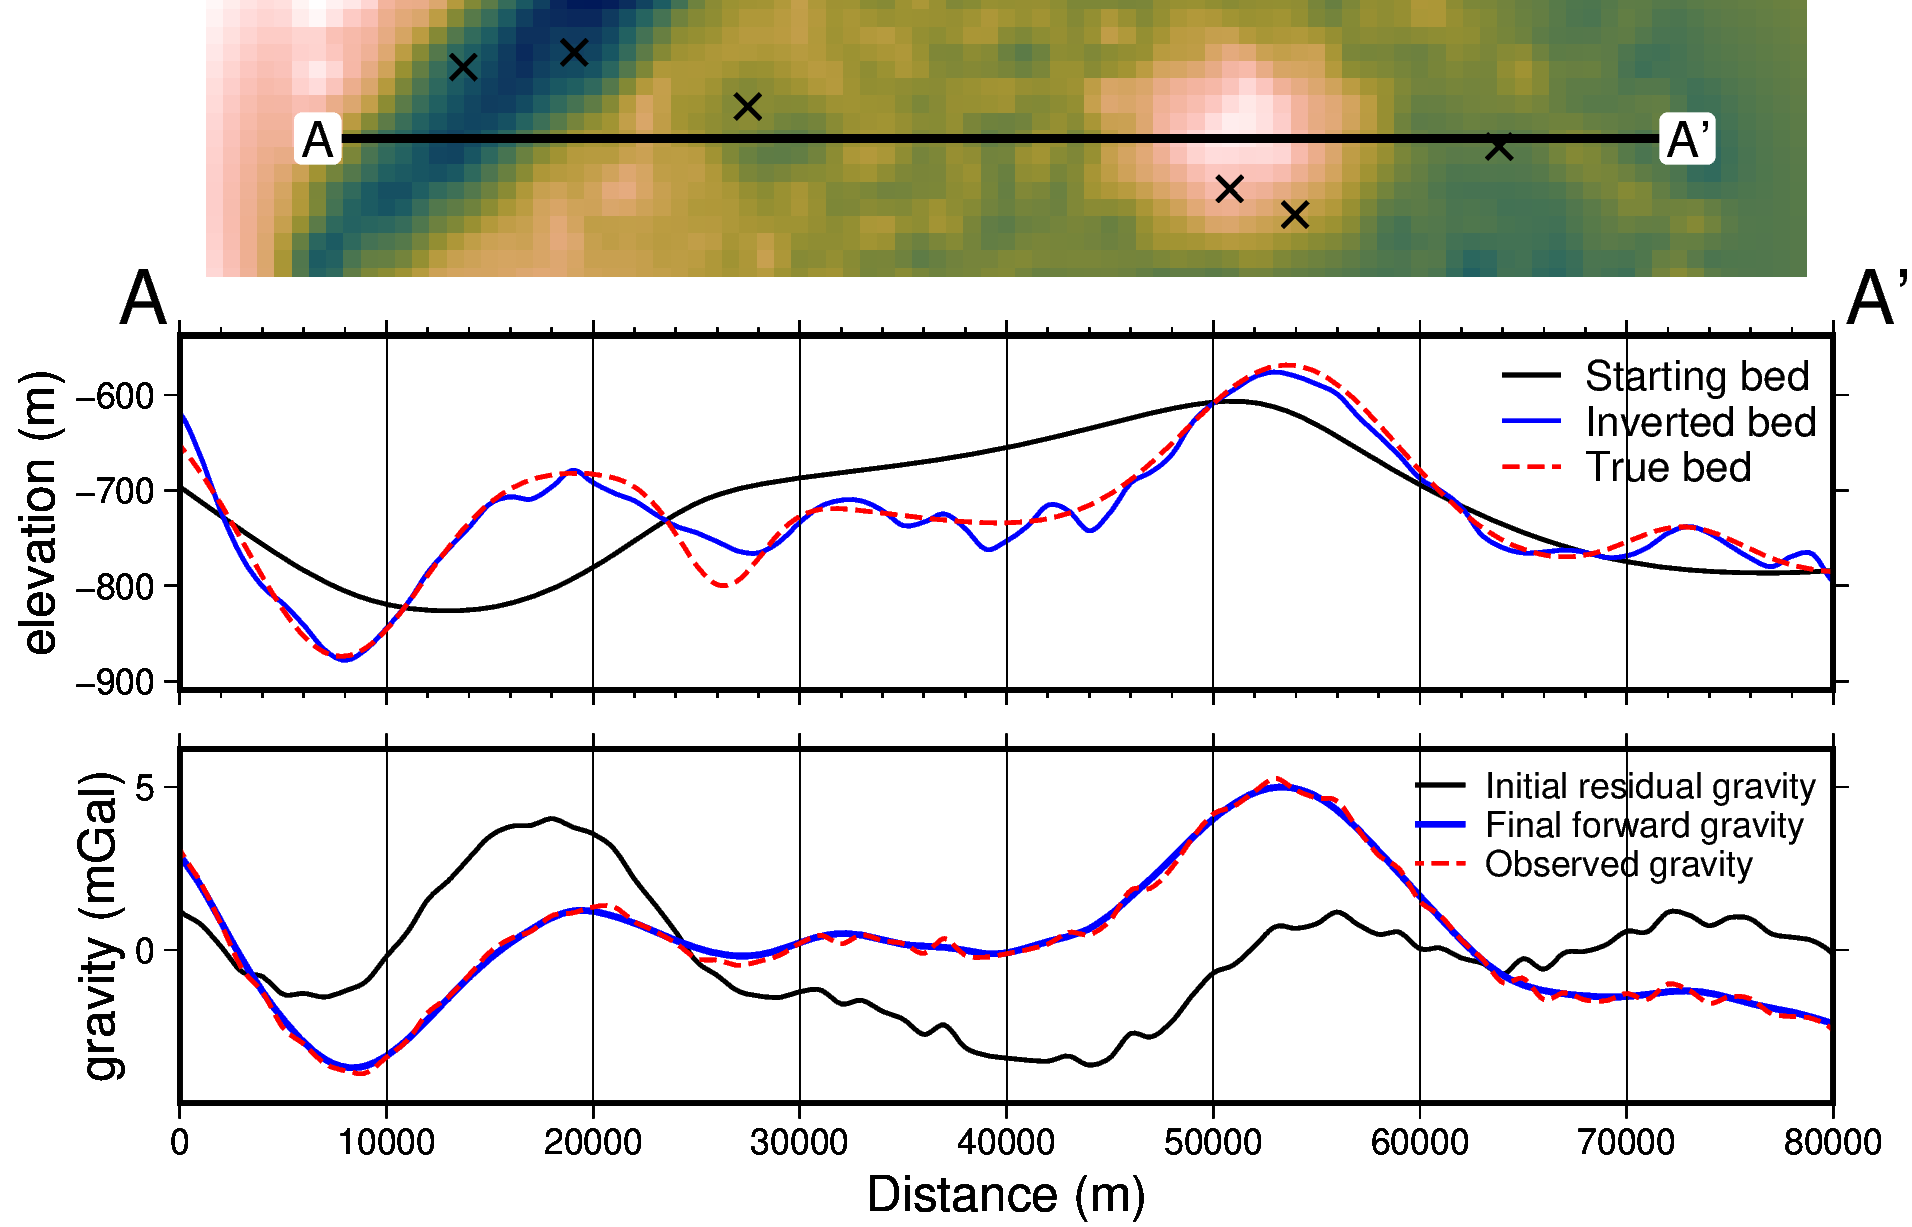
\includegraphics[width=\textwidth]{figures/chp3/chp3_simple_noise_profile.png}
        \caption{}
    \end{subfigure}
  \caption[Synthetic inversion with noise, CV and profile]{Cross-validation and profiles for the inversion with noise. \textbf{a)} Cross-validation curve showing the optimal damping parameter (red square). \textbf{b)} 2D profile of the inversion results. The top panel shows profile location and constraint points (black crosses). The middle panel contains topographic profiles of the starting, inverted, and true bathymetries. The bottom panel contains gravity anomaly profiles.}
    \label{fig:chp3_simple_noise_CV_and_profile}
\end{figure}

\subsubsection{Down-sampled data} \label{chp3:eq source resampled}
The previous two models used observed gravity data collected on a grid of observation points at the same grid spacing as the prism layer (1~km). This represents a very dense gravity survey. Gravity surveys are often relatively sparse compared to the resolution of the surface they are attempting to recover in an inversion. This section tests the effect of changing the resolution of the gravity data, to simulate a coarser gravity survey. Simply sampling the gravity data at a coarser resolution leads to a checker-boarding effect, where the inversion alters prisms nearby the gravity observations, but not prisms further away. 
For this reason, it is recommended here to re-grid the observed gravity data at a similar grid spacing to the prism layer. This can be accomplished with standard gridding techniques, such as minimum curvature or bi-harmonic splines (see section \ref{chp3_gridding_comparison}). However, these techniques aren't well suited for potential field data since they don't account for the variation in observation heights \citep{solergradientboosted2021}. An alternative method of interpolating the gravity data onto a finer resolution grid is the equivalent sources technique \citep{dampneyequivalent1969}\footnote{The equivalent sources technique is also used in this study as a means of regional separation (see section \ref{chp3_regional_seperation}, this is a similar application but for different purposes.}. \\

\begin{figure}[!ht]
\renewcommand\thesubfigure{\arabic{subfigure}}
  \centering
    \begin{subfigure}[t]{.95\textwidth}
        \centering
        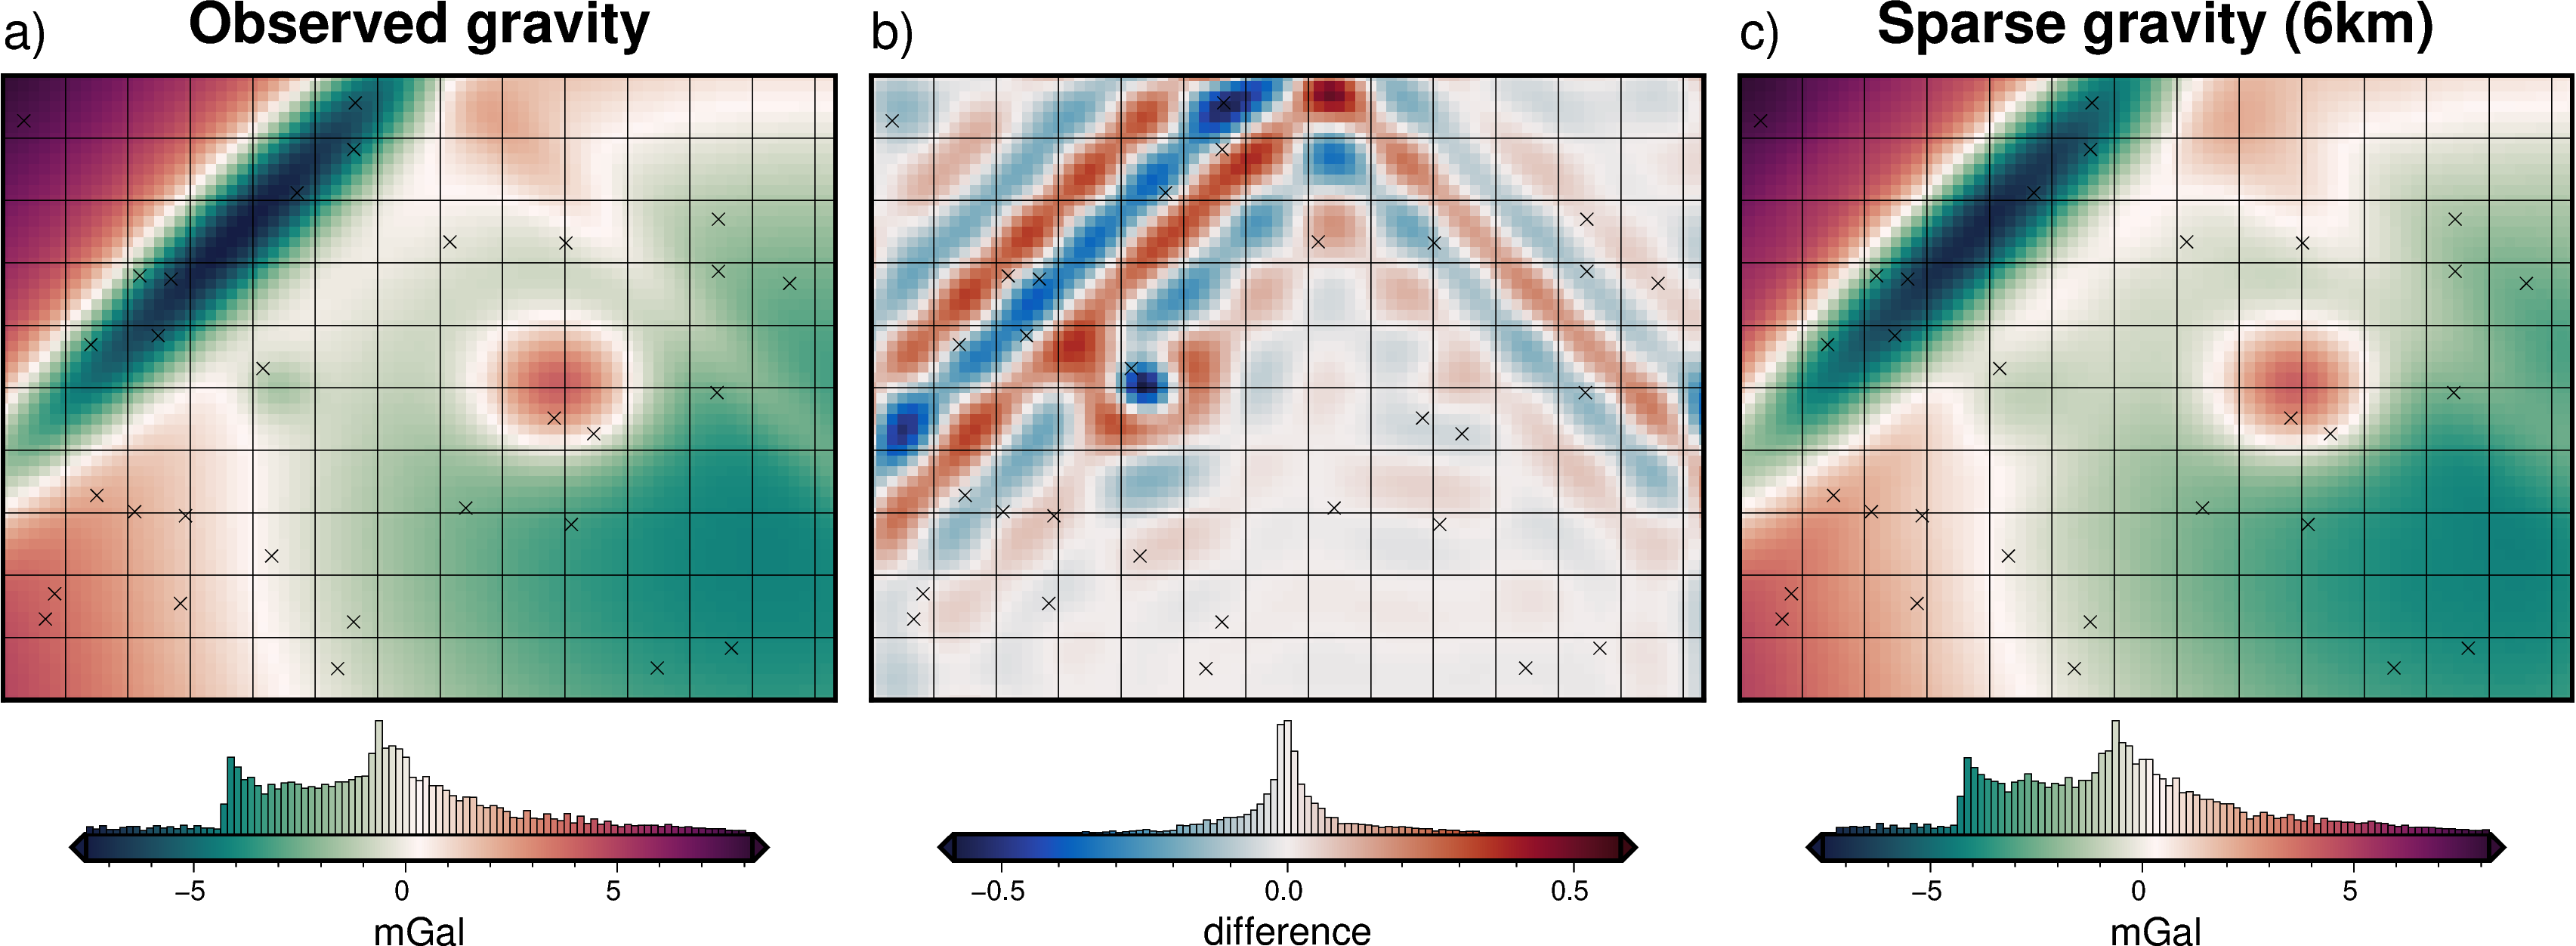
\includegraphics[width=\textwidth]{figures/chp3/chp3_simple_sampled_gravity_eq_sources.png}
        \caption{Equivalent sources re-gridding}
    \end{subfigure}
    \begin{subfigure}[t]{.95\textwidth}
        \centering
        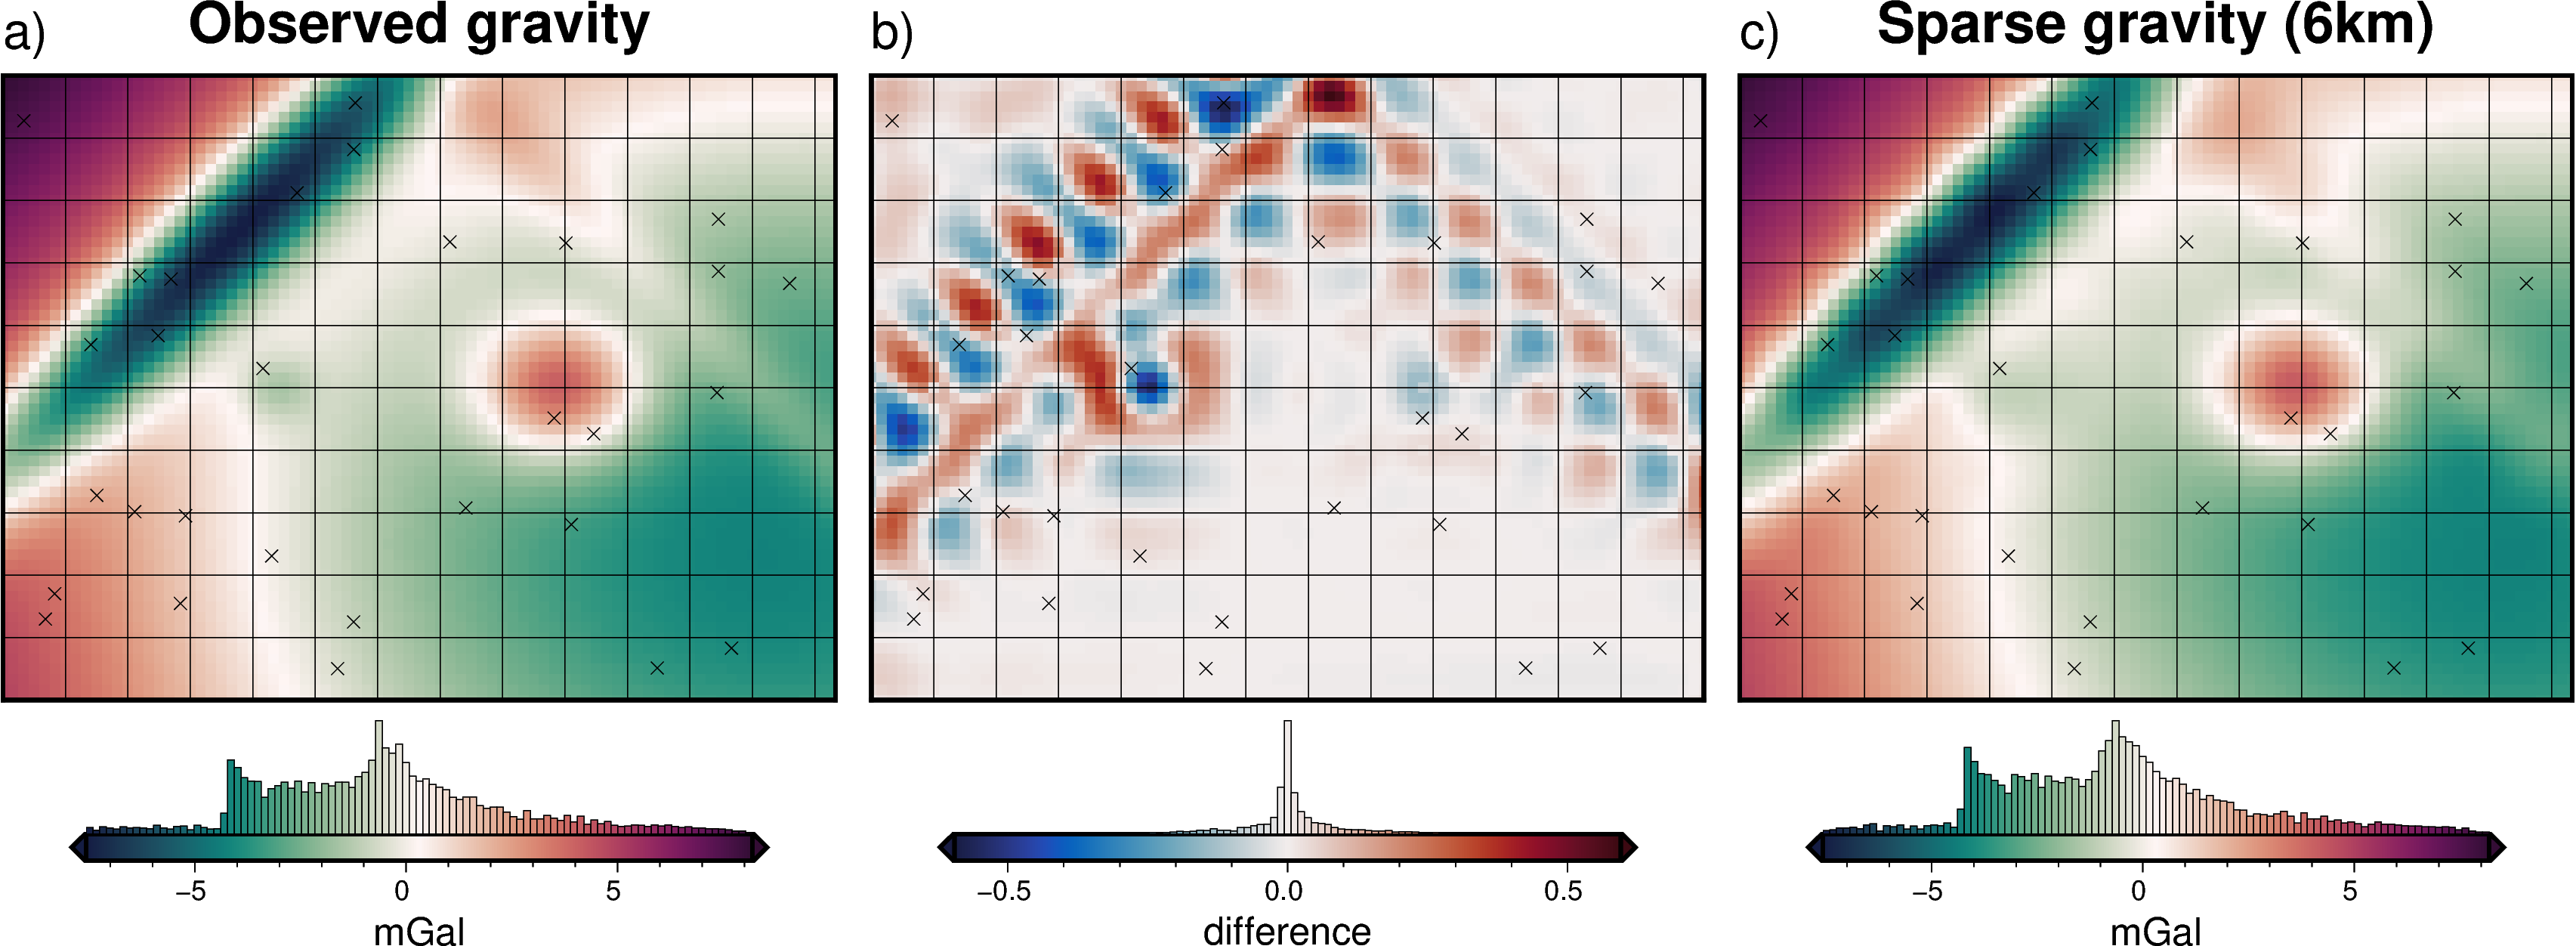
\includegraphics[width=\textwidth]{figures/chp3/chp3_simple_sampled_gravity_regular_gridding.png}
        \caption{Bi-harmonic spline re-gridding}
    \end{subfigure}
  \caption[Creating a low-resolution observed gravity survey]{Creating a low-resolution observed gravity survey. \textbf{Top panel} shows results using the equivalent source technique of gridding gravity data. \textbf{Bottom panel} shows simple gridding using a bi-harmonic spline. \textbf{a)} Original observed data on a 1~km grid, \textbf{b)} gravity signal lost due to sampling and re-gridding, \textbf{c)} the low-resolution observed gravity (6~km spacing) re-gridded at 1~km with either equivalent sources (top) or a regular gridding algorithm (bottom). Black crosses show constraint points and black lines show 6~km grid.}
    \label{fig:chp3_simple_eq_sources_regridding}
\end{figure}

Here, the original gravity data, on a 1~km grid, is sampled at a 6~km spaced grid to represent a low-resolution survey with observations every 6~km. A series of point sources are created at depth, and their densities are altered to best reproduce the observed gravity data. Once this process of fitting the source parameters to the data is accomplished, the gravity field can be predicted anywhere. For this application, the equivalent sources are predicted onto an even 1~km grid, to match the spacing of the bathymetry. Figure \ref{fig:chp3_simple_eq_sources_regridding} shows the results of this process (top panel) and the results using simple gridding without equivalent sources (bottom panel). \textit{Subplot a} shows the original observed gravity data (just training points) on a 1~km grid. This grid is sampled onto a 6~km grid (black grid lines) and re-gridded at 1~km (\textit{subplot c}). \textit{Subplot b} shows the difference, which represents the lost data resulting from the sparse survey. Typically the equivalent sources gridding technique is most beneficial to account for variations in observation heights. Here, even with constant elevations, there are noticeable differences between equivalent source gridding and simple gridding with bi-harmonic splines. \\

The equivalent-source resampled grid is used, with no added noise, in the same inversion procedure as the previous sections. The cross-validation (Figure \ref{fig:chp3_simple_sampled_CV_and_profile}a) resulted in an optimal damping value of 10\textsuperscript{-2}. The inverted bathymetry with this damping value is shown in Figure \ref{fig:chp3_simple_sampled_results}. The inversion was completed in 29~seconds and 38~iterations with a final RMS residual misfit of 0.019~mGal. The inversion was terminated due to the $\ell^2$-norm decreasing below the set threshold of 0.15~mGal\textsuperscript{1/2}. The inverted bathymetry had an RMS difference of 11 m with the true bathymetry and an RMS difference of 1~m at the constraint points. While the overall difference from the true bathymetry is low, this inversion failed to fully recover the small circular depression. Figure \ref{fig:chp3_simple_eq_sources_regridding} shows that the nearest observation point (intersection of gridlines) was on either side of this anomaly, and thus the sparse gravity survey used here failed to image the true magnitude of the feature. Figure \ref{fig:chp3_simple_sampled_results}b shows the absence of this feature in the inverted bathymetry. 

\begin{figure}[!ht]
    \centering
    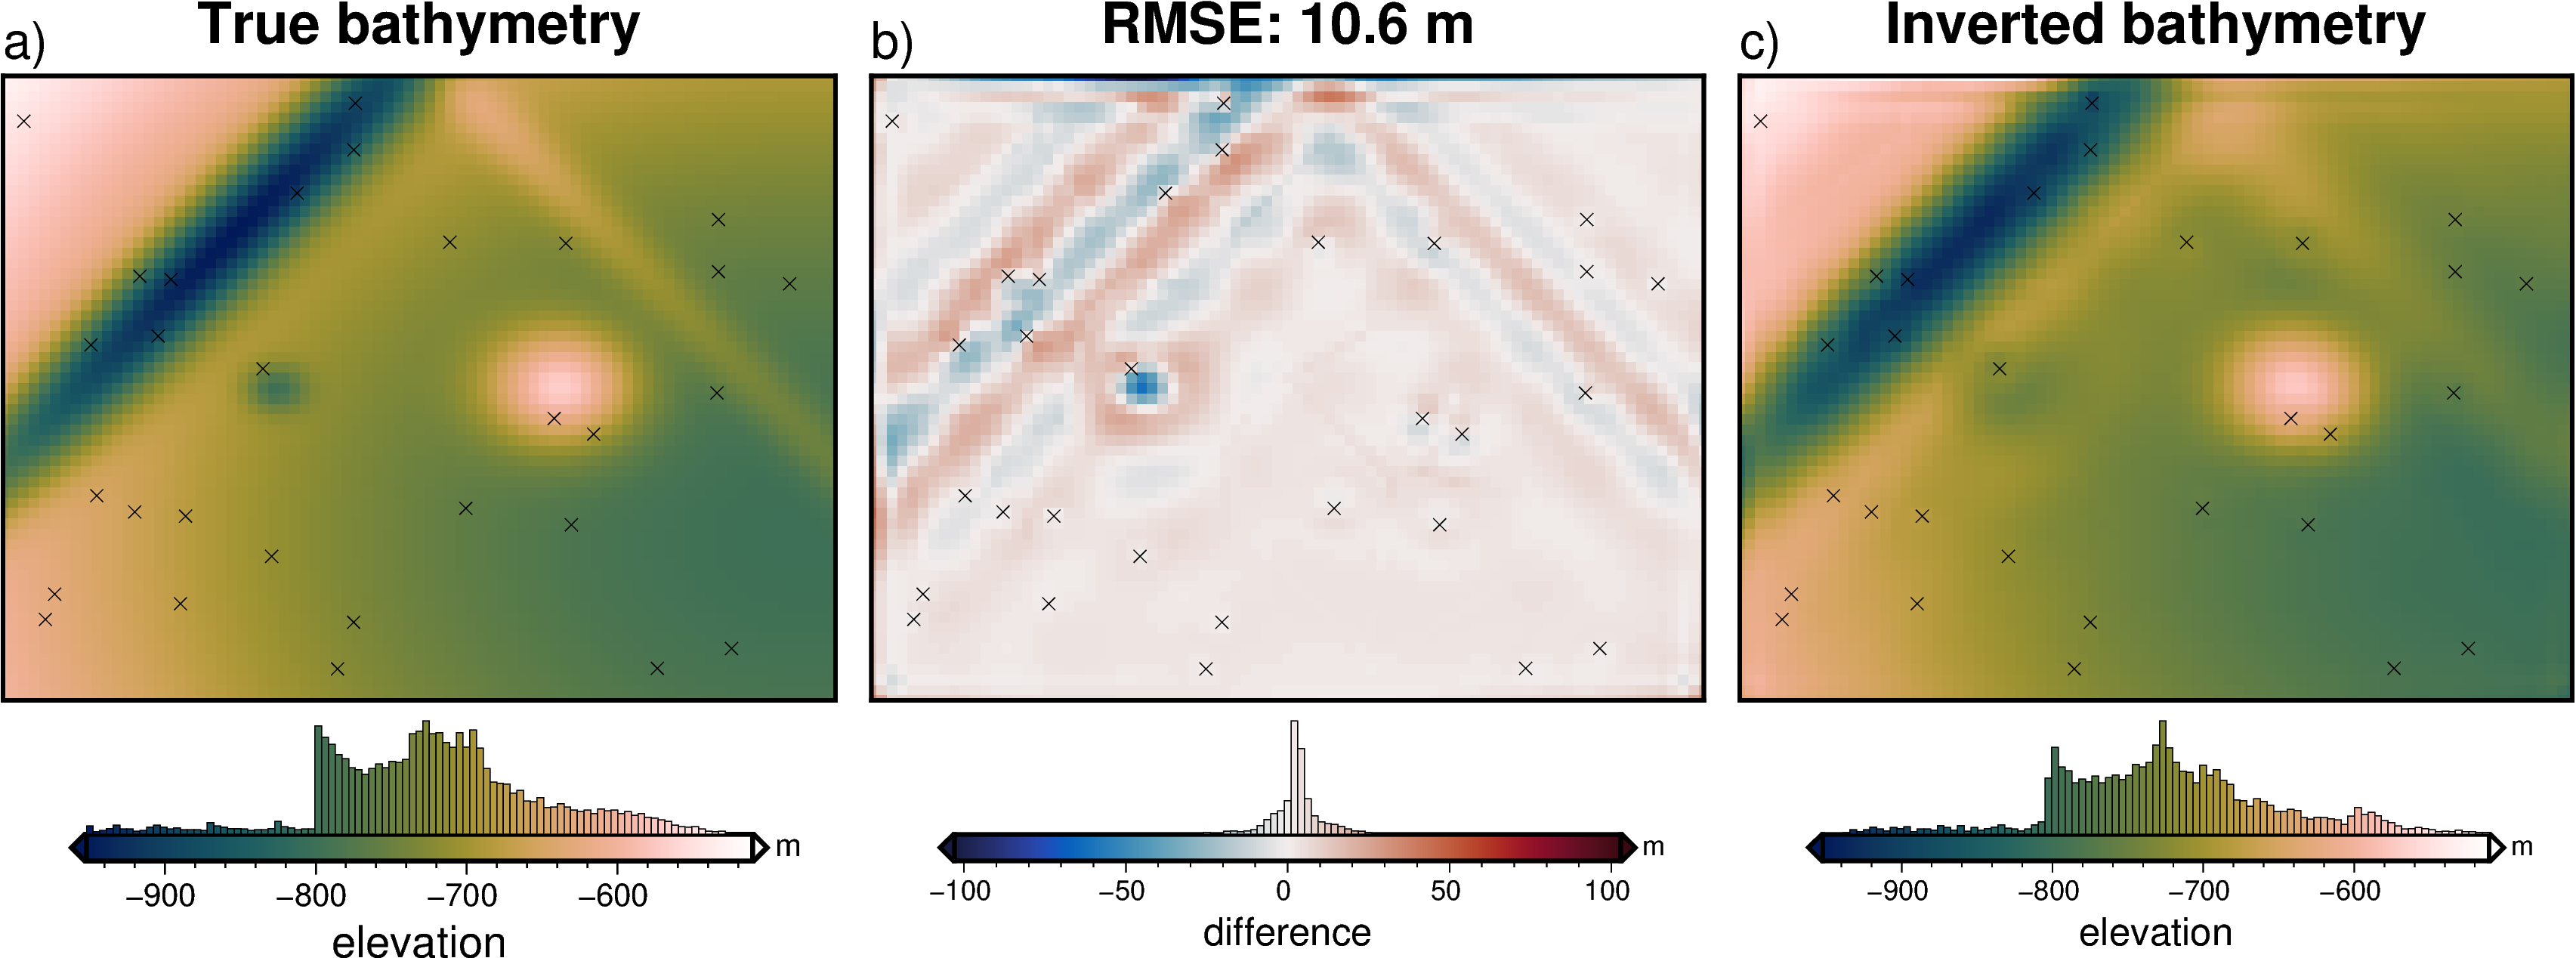
\includegraphics[width=0.95\textwidth]{chp3/chp3_simple_sampled_results}
    \caption[Synthetic inversion with sampled gravity]{Simple synthetic model inversion results with input data resampled at 6x the bathymetry grid spacing (6~km). \textbf{a)} True bathymetry, \textbf{b)} difference between a and c, and \textbf{c)} final inverted bathymetry. Black crosses show constraint points. The RMS difference with the true bathymetry at these constraints is 1~m.}
    \label{fig:chp3_simple_sampled_results}
\end{figure}

\begin{figure}[!ht]
  \centering
    \begin{subfigure}[t]{.40\textwidth}
        \centering
        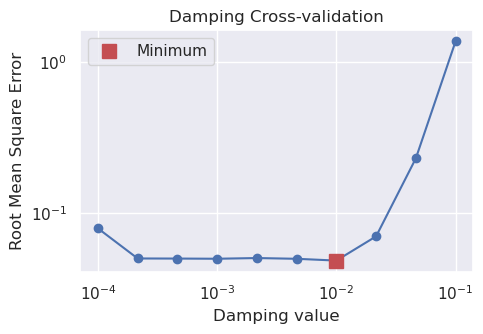
\includegraphics[width=\textwidth]{figures/chp3/chp3_simple_sampled_CV.png}
        \caption{}
    \end{subfigure}
    \begin{subfigure}[t]{.58\textwidth}
        \centering
        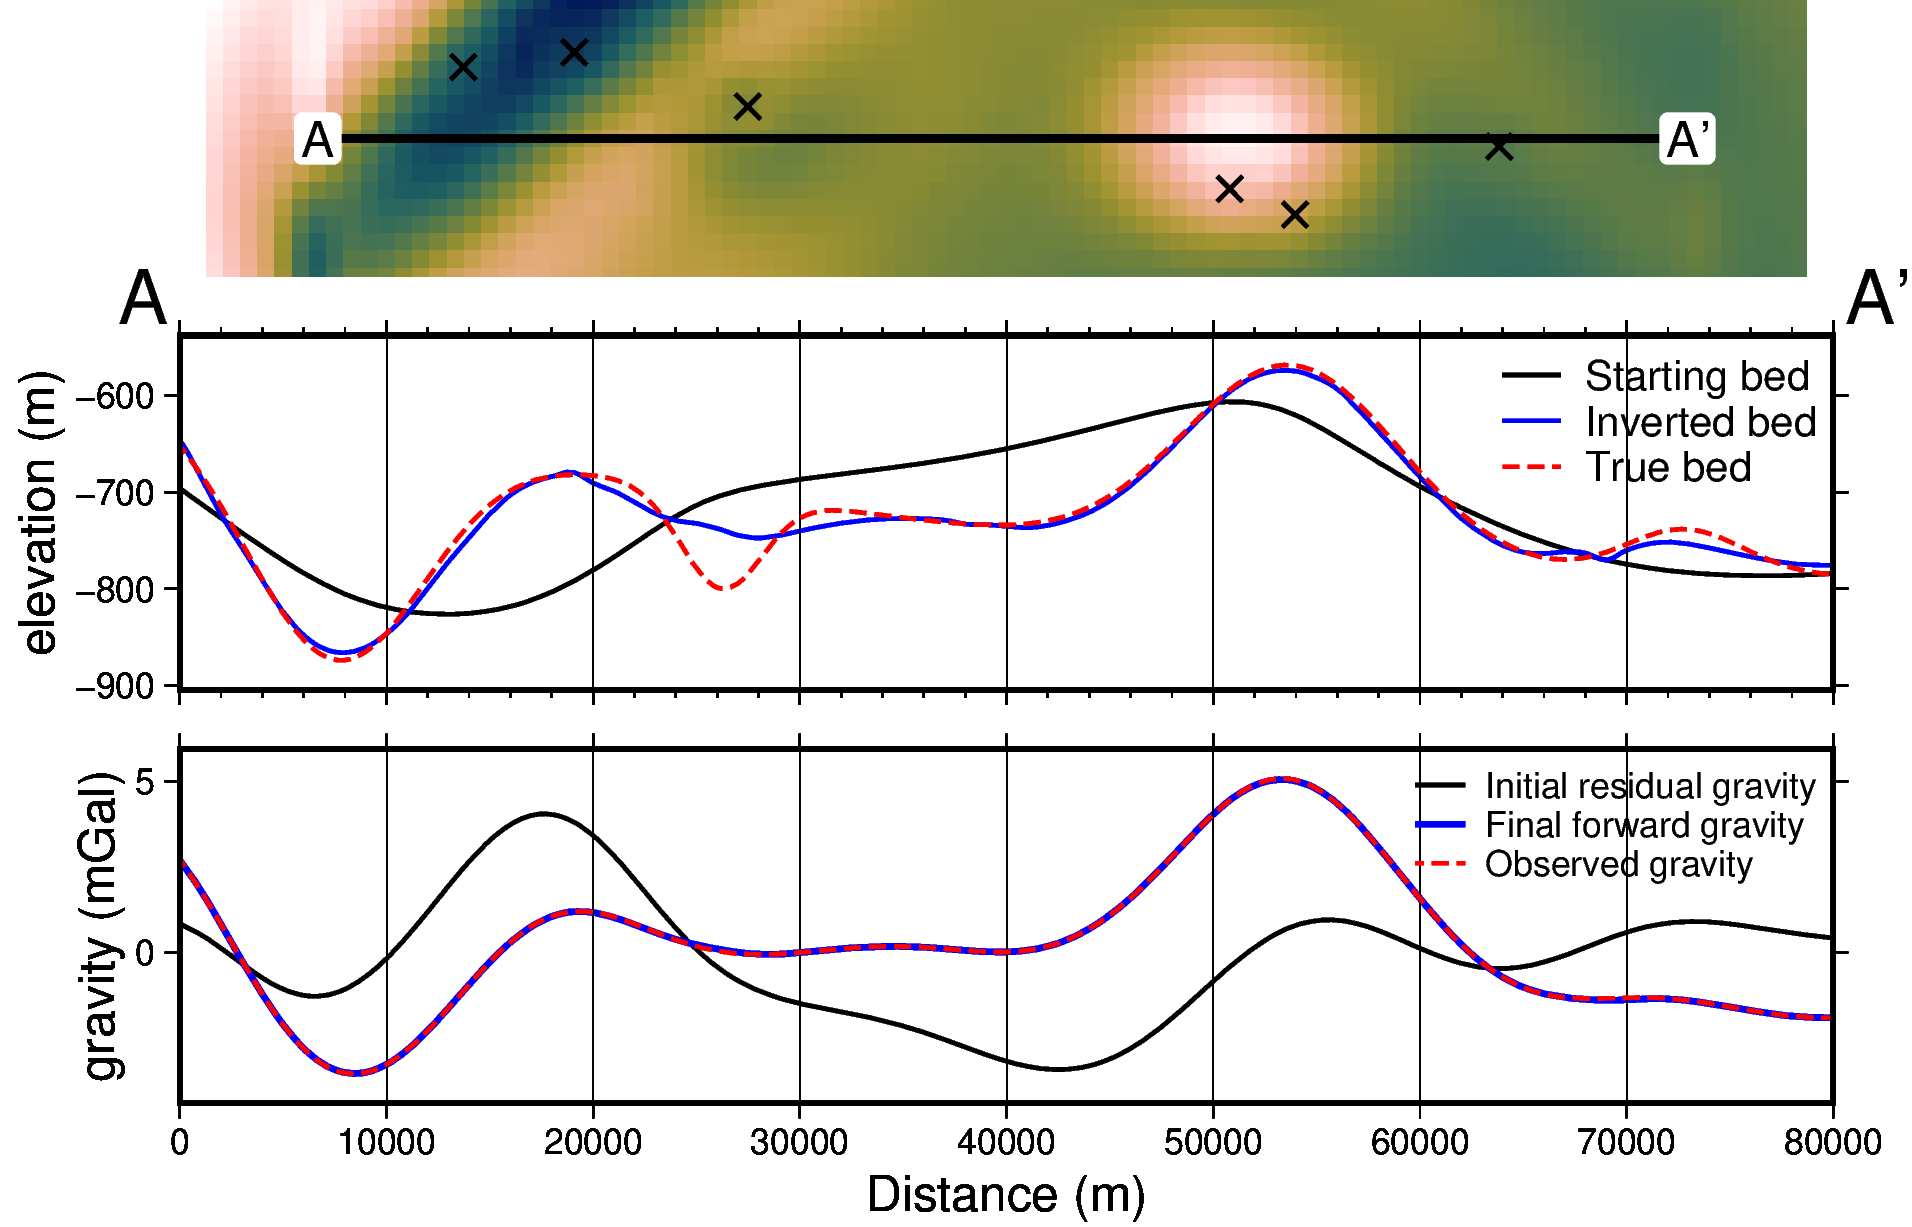
\includegraphics[width=\textwidth]{figures/chp3/chp3_simple_sampled_profile.png}
        \caption{}
    \end{subfigure}
  \caption[Synthetic inversion with sampled gravity, CV and profile]{Cross-validation and profiles for the 6~km resampled inversion. \textbf{a)} Cross-validation curve showing the optimal damping parameter. \textbf{b)} 2D profile of the inversion results. The top panel shows profile location and constraint points (black crosses). The middle panel contains topographic profiles of the starting, inverted, and true bathymetries. The bottom panel contains gravity anomaly profiles.}
    \label{fig:chp3_simple_sampled_CV_and_profile}
\end{figure}

\subsection{Ensemble of Noise and Sampling values} \label{chp3:simple_ensemble}

\begin{figure}[!ht]
    \centering
    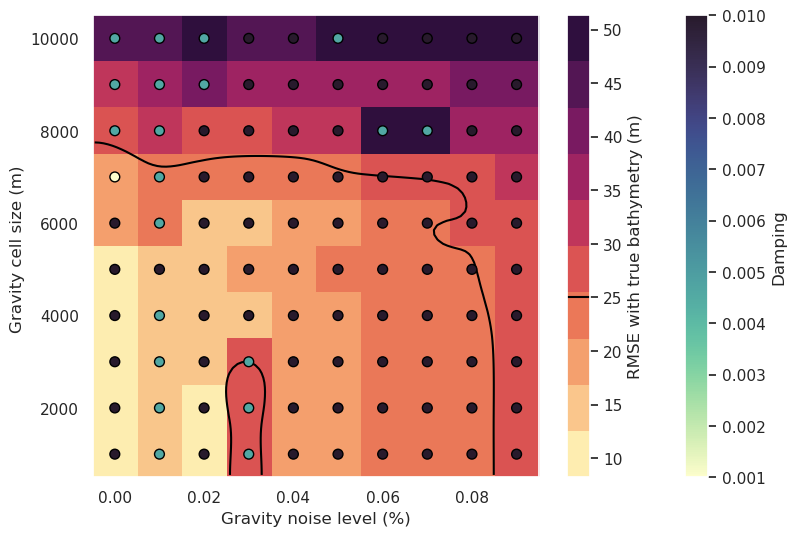
\includegraphics[width=0.9\textwidth]{figures/chp3/chp3_simple_ensemble.png}
    \caption[Gravity data ensemble for synthetic model]{Ensemble of noise levels and gravity spacing for the simple synthetic model. Grid cell colour indicates each inversion's RMS difference with the true bathymetry. The circles' colour indicates the optimal damping value found for each inversion's cross-validation. Black line shows the 25~m RMSE contour, indicative of the amplitude of the smallest amplitude features.}
    \label{fig:chp3_simple_ensemble}
\end{figure}

To test the relative importance of the level of noise and the resolution of the gravity data (i.e. station/flight line spacing), an ensemble of 100 inversions was run, with 10 noise levels between 0 and 9\%, and 10 gravity resolutions between 1 and 10~km. The noise level percentages are of the maximum absolute value of the data, equating to 10 levels between 0 and 0.85~mGal. The differing gravity resolutions were created with the sampling and re-gridding of equivalent sources outlined in the above section. For each set of noise and spacing values, the cross-validation routine was used to find the optimal damping parameters and associated inverted bathymetries. Each of these 100 inversions were then compared to the true bathymetry yielding an RMS difference for each. 

Figure \ref{fig:chp3_simple_ensemble} shows the results of this ensemble of inversion. Each grid cell represents a single inversion, with the level of noise and gravity resolution for the inversion indicated by the x and y axis, respectively. The background colour (warm colours) indicates each inversion's resulting RMS difference with the true bathymetry. Coloured circles show the optimal damping value for each inversion found through cross-validation. This shows a general decrease in the inversion's accuracy with either more noise or lower-resolution gravity data. The smallest bathymetric features which this inversion ideally should recover have amplitudes of tens of meters (small circular depression and narrow ridge). The RMSE here indicates a base-level of error in the inversions, while the error in the vicinity of the short wavelength bathymetry features is likely higher (Figure \ref{fig:chp3_simple_sampled_results}b). Inversions with RMSEs of 10's of meters will likely fail to resolve these small features. For this inversion, an RMSE of 25~m (black contour in Figure \ref{fig:chp3_simple_ensemble}) approximately equates to a gravity observation spacing greater than 8 times the prism layer spacing, and a noise level higher than 8\% of the survey's max absolute value.

\section{Adding a regional component} \label{chp3:simple_regional_model}

Now that the inversion has been demonstrated to adequately recover bathymetry with various levels of noise and resolutions of the input gravity data, an additional complexity is added. This complexity is a regional component of the observed gravity field. To account for this, the inversion remains the same, but the regional component of the gravity misfit must be removed beforehand (Equation \ref{eq:regional_residual}). In this section, first, the four methods of regional separation laid out in \ref{chp3_regional_seperation} are compared. Next, one of these methods, constraint point minimization, is further investigated. Lastly, the effects of noise and gravity survey spacing are explored. 

\begin{figure}[!ht]
    \centering
    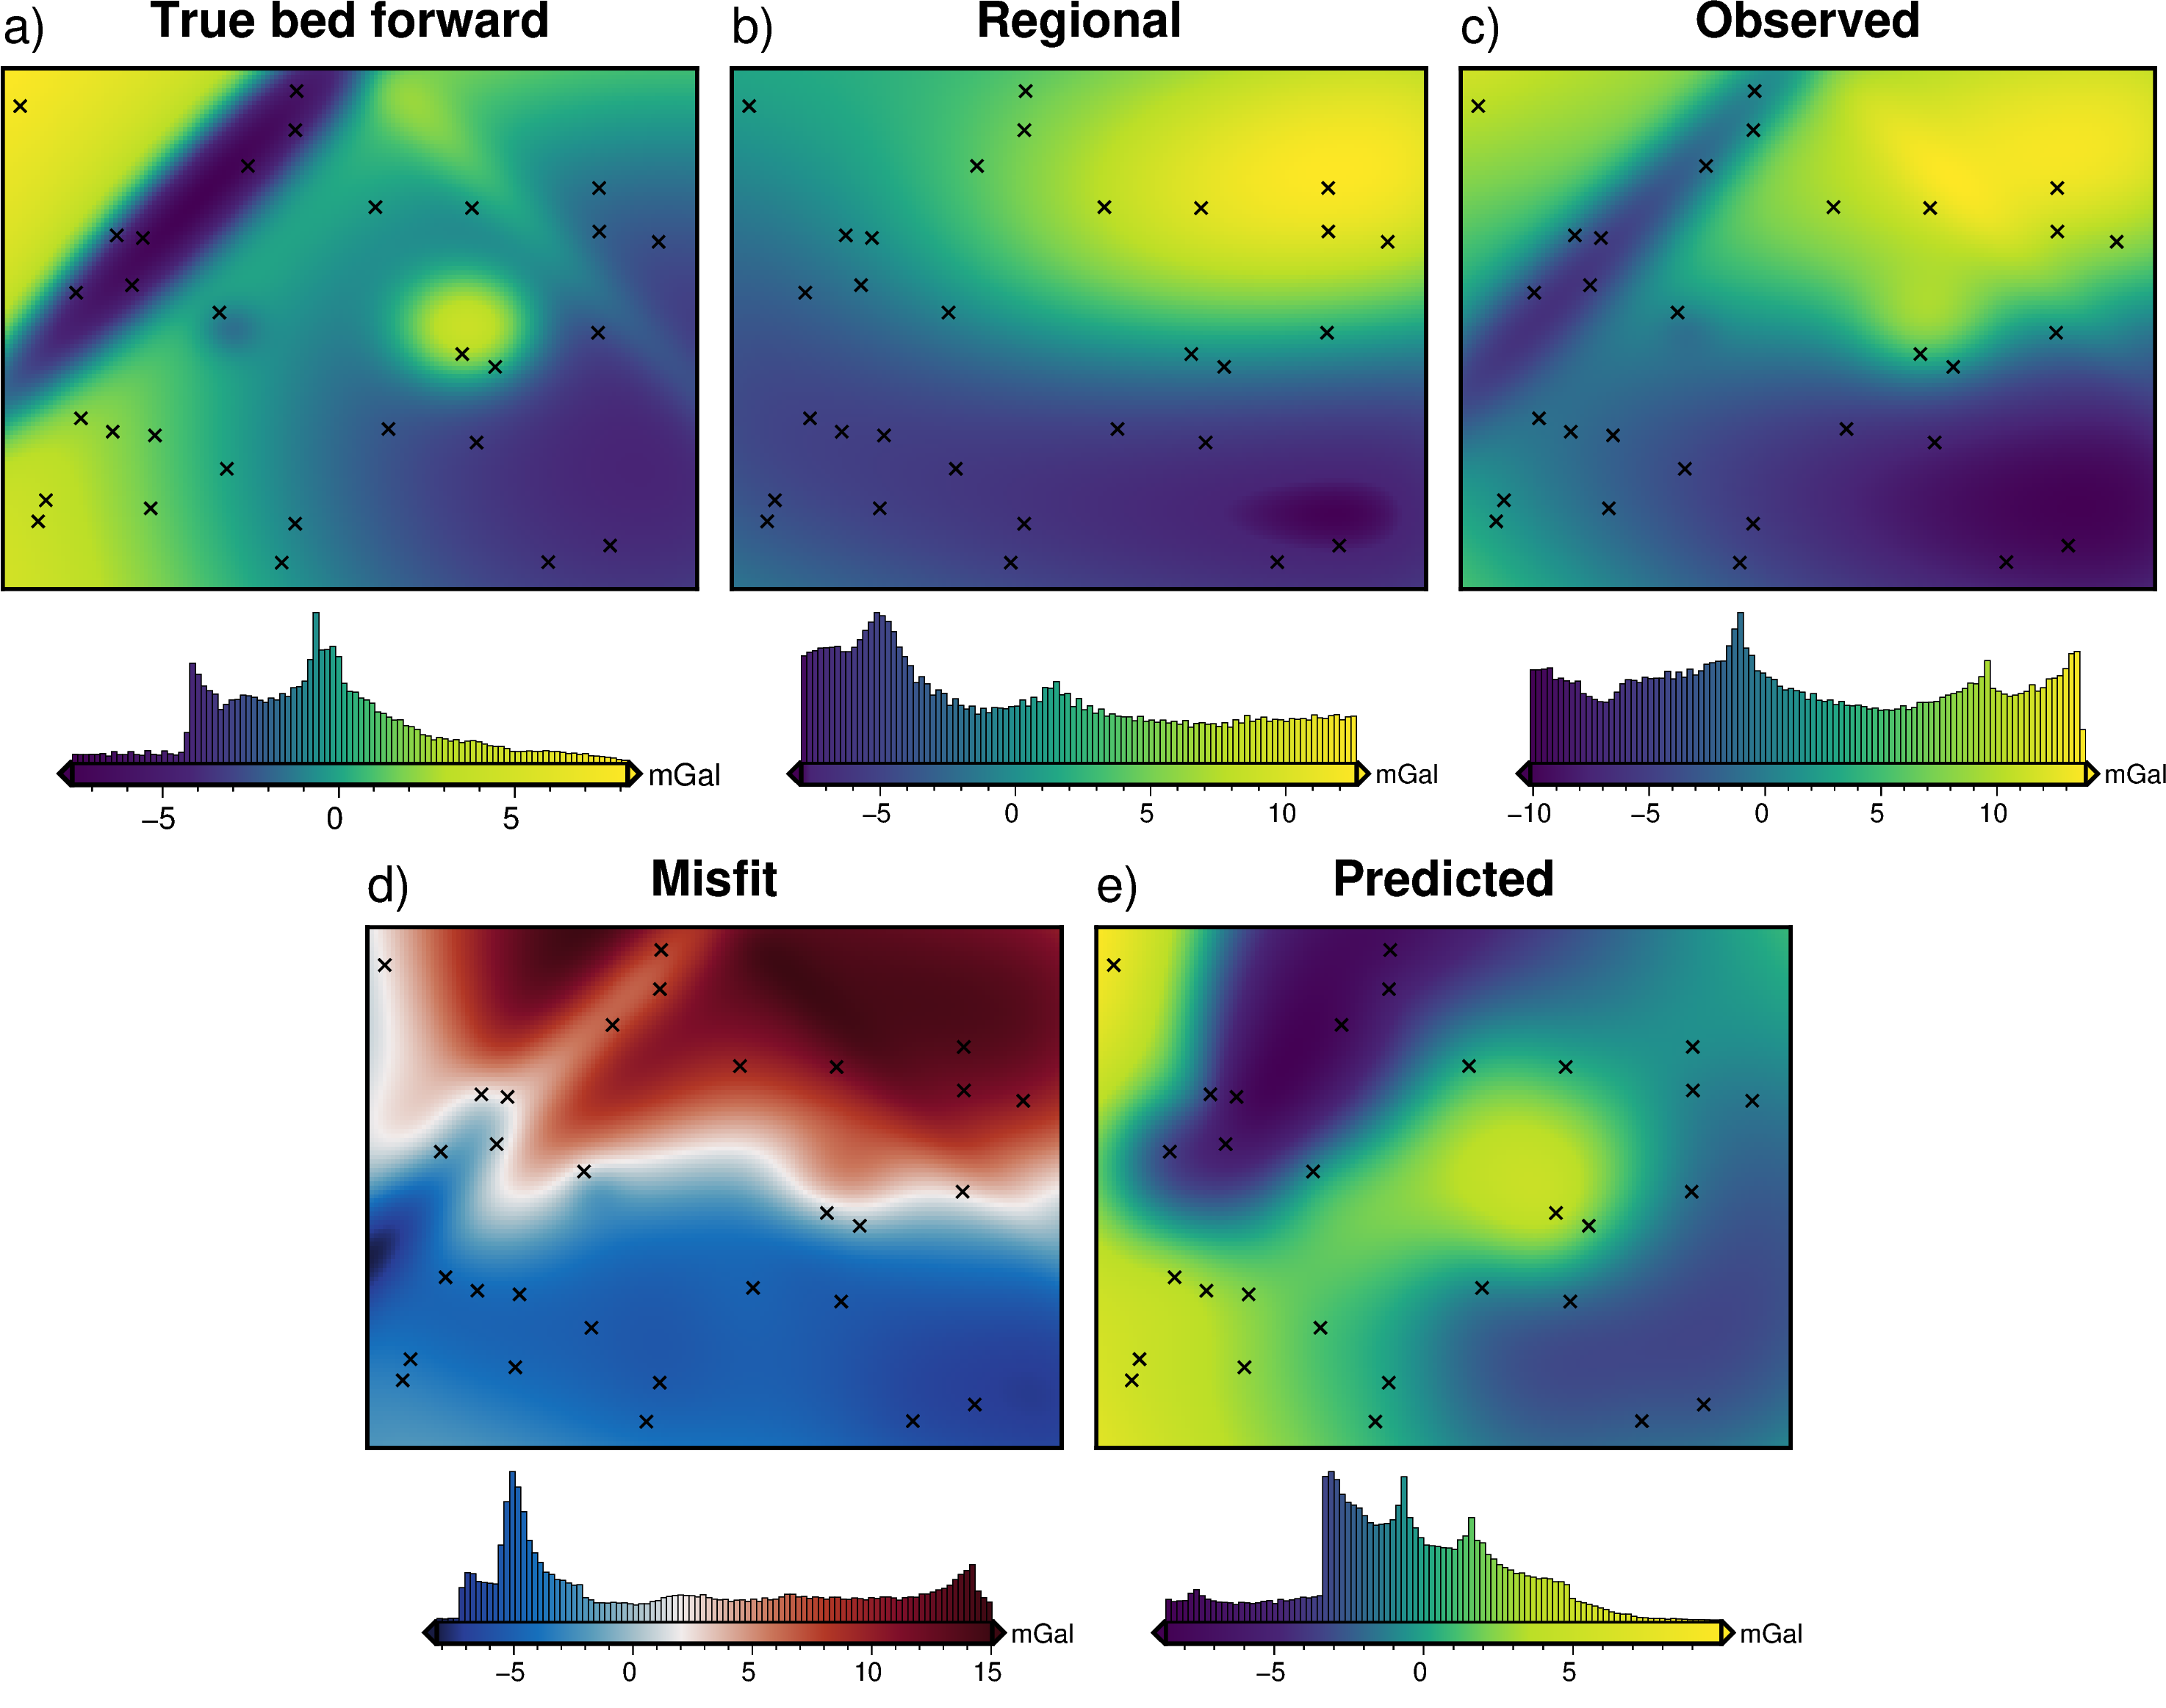
\includegraphics[width=0.95\textwidth]{figures/chp3/chp3_simple_regional_gravity.png}
    \caption[Gravity anomalies with a regional field]{Gravity components and anomalies for the simple synthetic model with the addition of a regional field. \textbf{a)} the forward gravity of the true bathymetry, \textbf{b)} the regional component of gravity, \textbf{c)} the observed gravity from the combination of a and b, \textbf{d)} the gravity misfit from the difference between c and e, and \textbf{e)} the predicted gravity from the forward calculation of the starting bathymetry.}
    \label{fig:chp3_simple_regional_gravity}
\end{figure}

This model uses the same starting bathymetry (Figure \ref{fig:chp3_simple_starting_model}) as the previous section, but the observed gravity includes a regional field, which represents the portion of observed gravity signal resulting from unknown crustal sources, such as anomalous bodies or crustal thickness variations. This component (Figure \ref{fig:chp3_simple_regional_gravity}b) is calculated from a synthetic topography with a median elevation of -4300~m and a density contrast of 700~kg~m\textsuperscript{-1}. Its range of gravity values is set to be the dominant signal in the observed gravity, but not large enough to fully mask the signal of the bathymetry signal. Figure \ref{fig:chp3_simple_regional_gravity} shows the various components of the gravity and resulting misfit for this model. 

\subsection{Regional separation methods}

The four methods of regional separation discussed in section \ref{chp3_regional_seperation} each have at least one hyper-parameter which affects their calculation of the regional field. For each method these include 
\begin{enumerate}
    \item Low-pass filter: the distance width of the Gaussian filter.
    \item Trend removal: the degree of the polynomial trend fit to the misfit.
    \item Equivalent source prediction: the depth and damping parameters of fitting sources to the data \citep{solergradientboosted2021}.
    \item Constraint point minimization: parameters for the associated gridding method, such as the tension factor for minimum curvature gridding \citep{smithgridding1990} or the minimum distance and damping parameter for bi-harmonic spline gridding \citep{uiedaverde2018}.
\end{enumerate}

\begin{figure}[!ht]
    \centering
    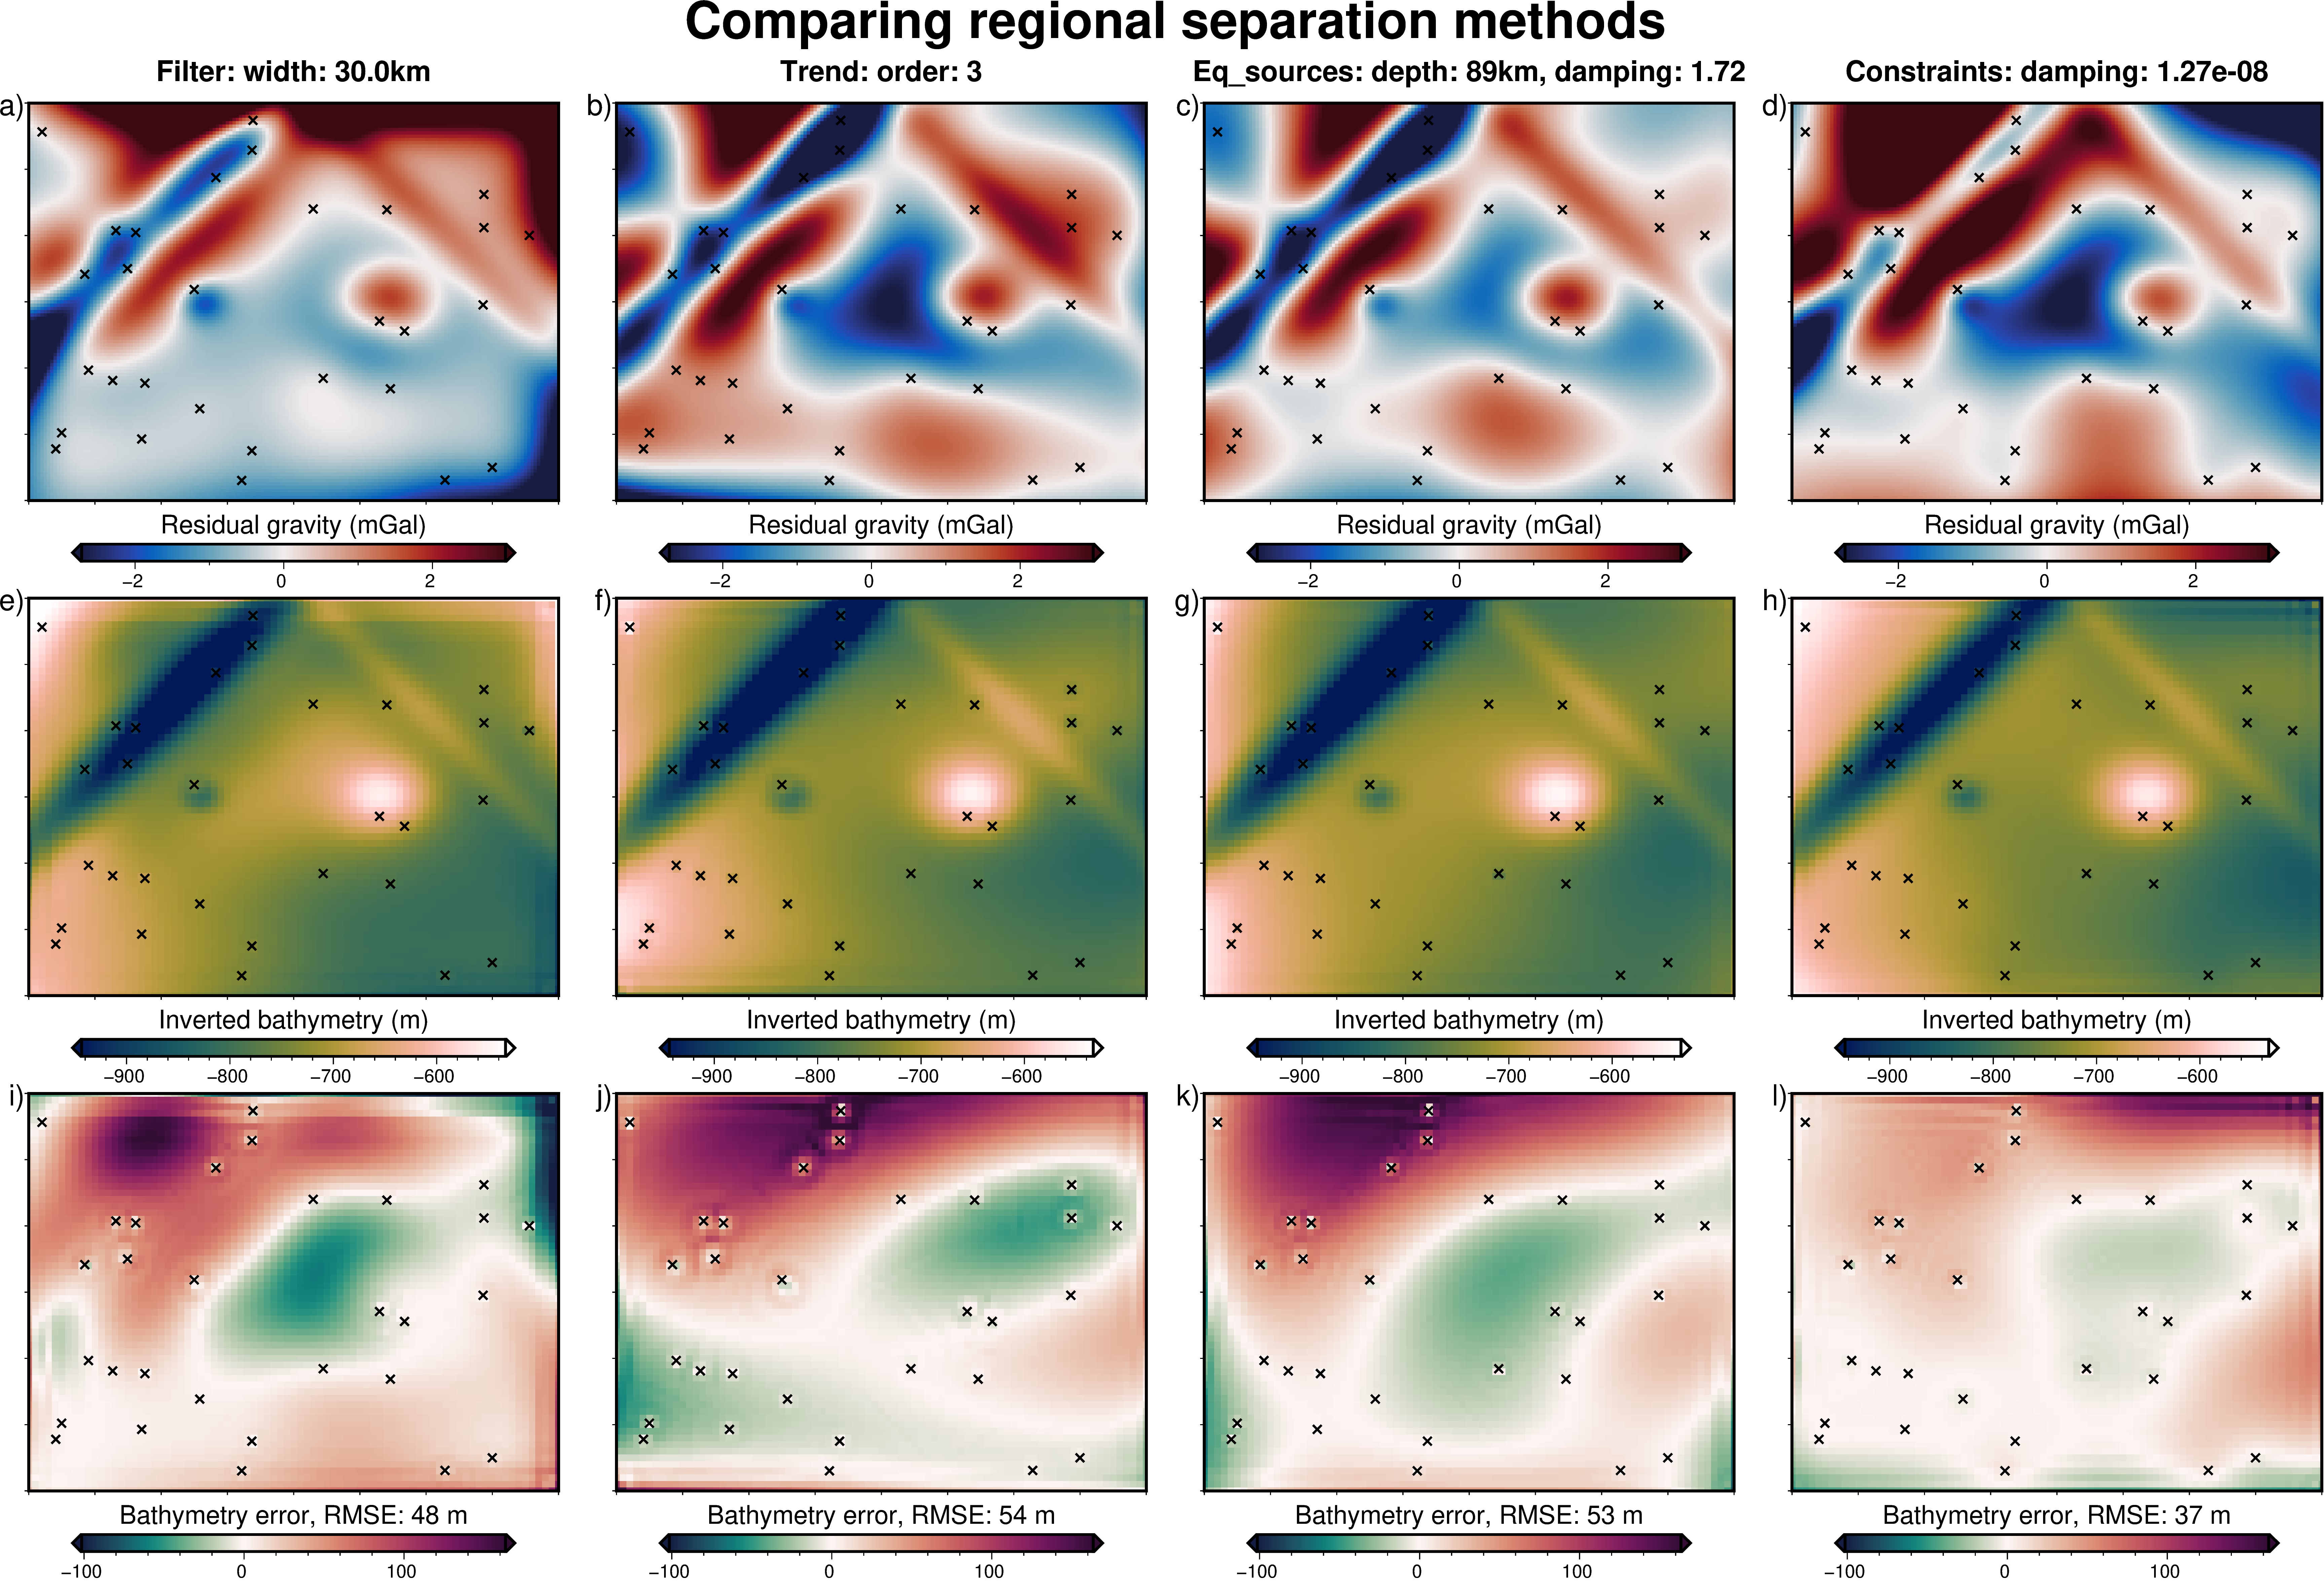
\includegraphics[width=1\textwidth]{figures/chp3/chp3_simple_regional_comparison.png}
    \caption[Regional separation methods]{Comparison of inversions with 4 regional separation methods. First row (\textbf{a-d}) shows residual gravity misfit after regional separation. Second row (\textbf{e-h}) shows the inverted bathymetry for each method. Third row (\textbf{i-l}) shows the error of the inverted bathymetries with the true bathymetry. Constraint points are shown as black crosses. Colourmaps are identical for each row. Profiles of these data are shown in Figure \ref{fig:appB_simple_regional_comparison_profile} of Appendix \ref{appendix:B}.}
    \label{fig:chp3_simple_regional_comparison}
\end{figure}

Since for this synthetic model, the true regional field is known (Figure \ref{fig:chp3_simple_regional_gravity}b), the effect of the parameters associated with each of the four methods can be explored. Excluding the constraint point minimization method, an optimization is run for each method, with the goal of finding the parameter values which minimize the RMS difference between the true and calculated regional gravity. Each optimization has 20 trials. The constraint point minimization doesn't require optimization because the various gridding parameters won't significantly affect the RMS difference between the resulting regional field and the true field. However, the gridding parameters will affect the inversion itself; this is explored in the next section. For this comparison of the regional removal method, the constraint point minimization method uses bi-harmonic spline grinding, and the gridding damping parameter is chosen with a cross-validation \citep{uiedaverde2018}. The best regional field (lowest RMS with the true regional field) of each method was found with the following parameters: 
\begin{enumerate}
    \item a 30~km filter width for the low pass filter method
    \item a 3\textsuperscript{rd} order trend for the trend removal method
    \item source depth of 89~km and a damping value of 1.72 for the equivalent source technique
    \item an interpolator damping of $1.27x10^{-8}$ for the bi-harmonic spline interpolator of the constraint point minimization method. 
\end{enumerate}

Each of these regional fields was then removed from the gravity misfit, producing the residual anomalies (Figure \ref{fig:chp3_simple_regional_comparison}a-d). These resulting residuals were then input into an inversion, resulting in the inverted bathymetries of d-h of Figure \ref{fig:chp3_simple_regional_comparison}, and the bathymetry error relative to the true bathymetry was found (Figure \ref{fig:chp3_simple_regional_comparison}i-l). For these inversions, the same damping parameter cross-validation was conducted, as described in Section \ref{chp3:simple_model_CV}. This comparison of regional separation methods shows that the constraint point minimization method (Figure \ref{fig:chp3_simple_regional_comparison}l) produces the best inverted bathymetry, both visually (Figure \ref{fig:chp3_simple_regional_comparison}h), and based on the RMS difference with the true bathymetry (37~m). Figure \ref{fig:appB_simple_regional_comparison_profile} in Appendix \ref{appendix:B} shows a profile of the resulting regional fields and inverted bathymetries of these various methods of regional separation. The remainder of this section further examines the constraint point minimization method of regional separation.

\subsection{Constraint point minimization} \label{chp3_gridding_comparison}
The constraint point minimization method assumes that at locations of known bathymetry, there is no residual component of gravity misfit, and the regional component entirely equals the misfit. To implement this, misfit values at the constraints are sampled and used to create a region-wide grid of regional values. This grid is then removed from the misfit to get the residual misfit (Equation \ref{eq:regional_residual}). This gridding can be accomplished by many techniques, which at an initial inspection appear to produce similar results. Here, two methods of gridding and their gridding parameters are compared, and the impact on the inverted bathymetry are shown. These gridding methods are tensioned minimum curvature \citep{smithgridding1990} and bi-harmonic splines \citep{sandwellbiharmonic1987}. 

\subsubsection{Tensioned minimum curvature}
Tensioned minimum curvature gridding is a commonly used technique for gridding sparse data which fits the smoothest possible surface while still matching the data \citep{wesselinterpolation1998}. It allows variation in the location of maximum curvature through the tension factor parameter. A tension factor of 0 results in the minimum curvature solution (maxima and minima allowed anywhere), while a value of 1 localizes the curvature at the data points (maxima or minima only allowed at the data points) \citep{smithgridding1990}. A tension of 0.25 is suggested for potential field data \citep{wesselgeneric2019}. Tensioned minimum curvature has been used in several bathymetric inversions for constraint point minimization \citep{yangbathymetry2021, millanconstraining2020, anbathymetry2019}. 

\subsubsection{Bi-harmonic splines}
The second method of gridding the sampled gravity misfit values uses bi-harmonic splines. This method uses Green's functions and the least squares fit to the data \citep{sandwellbiharmonic1987}. Computation time for this technique is approximately proportional to the cube of the number of data, making it computationally expensive for large datasets \citep{dengmoving2011}. There is a damping parameter value that can be adjusted, to smooth the resulting interpolation. As implemented in the \textit{SplineCV} class of the Python package Verde \citep{uiedaverde2018}, automated cross-validation of the data can be used to identify the damping value which  best predicts the data. Once the parameter is determined, and the data is interpolated, the interpolation can be predicted at any location, such as on the nodes of a uniform grid. \\

Despite its slow run time with large datasets, bi-harmonic spline gridding has several advantages over tensioned minimum curvature gridding. It allows the incorporation of data uncertainties into the fitting via a weighting parameter. With the use of cross-validation, there are no subjective parameters that can significantly alter the results. Lastly, the predicted data don't need to be on a regular grid, which is useful for irregularly shaped domains that don't adhere to a rectangular region. In their bathymetry inversion, \citet{millanconstraining2020} point out features in their inverted bathymetry which likely result from the minimum curvature gridding technique. Apart from this, there appears to be little work related the how the gridding procedure affects this aspect of a bathymetry inversion.

\begin{figure}[!ht]
    \centering
    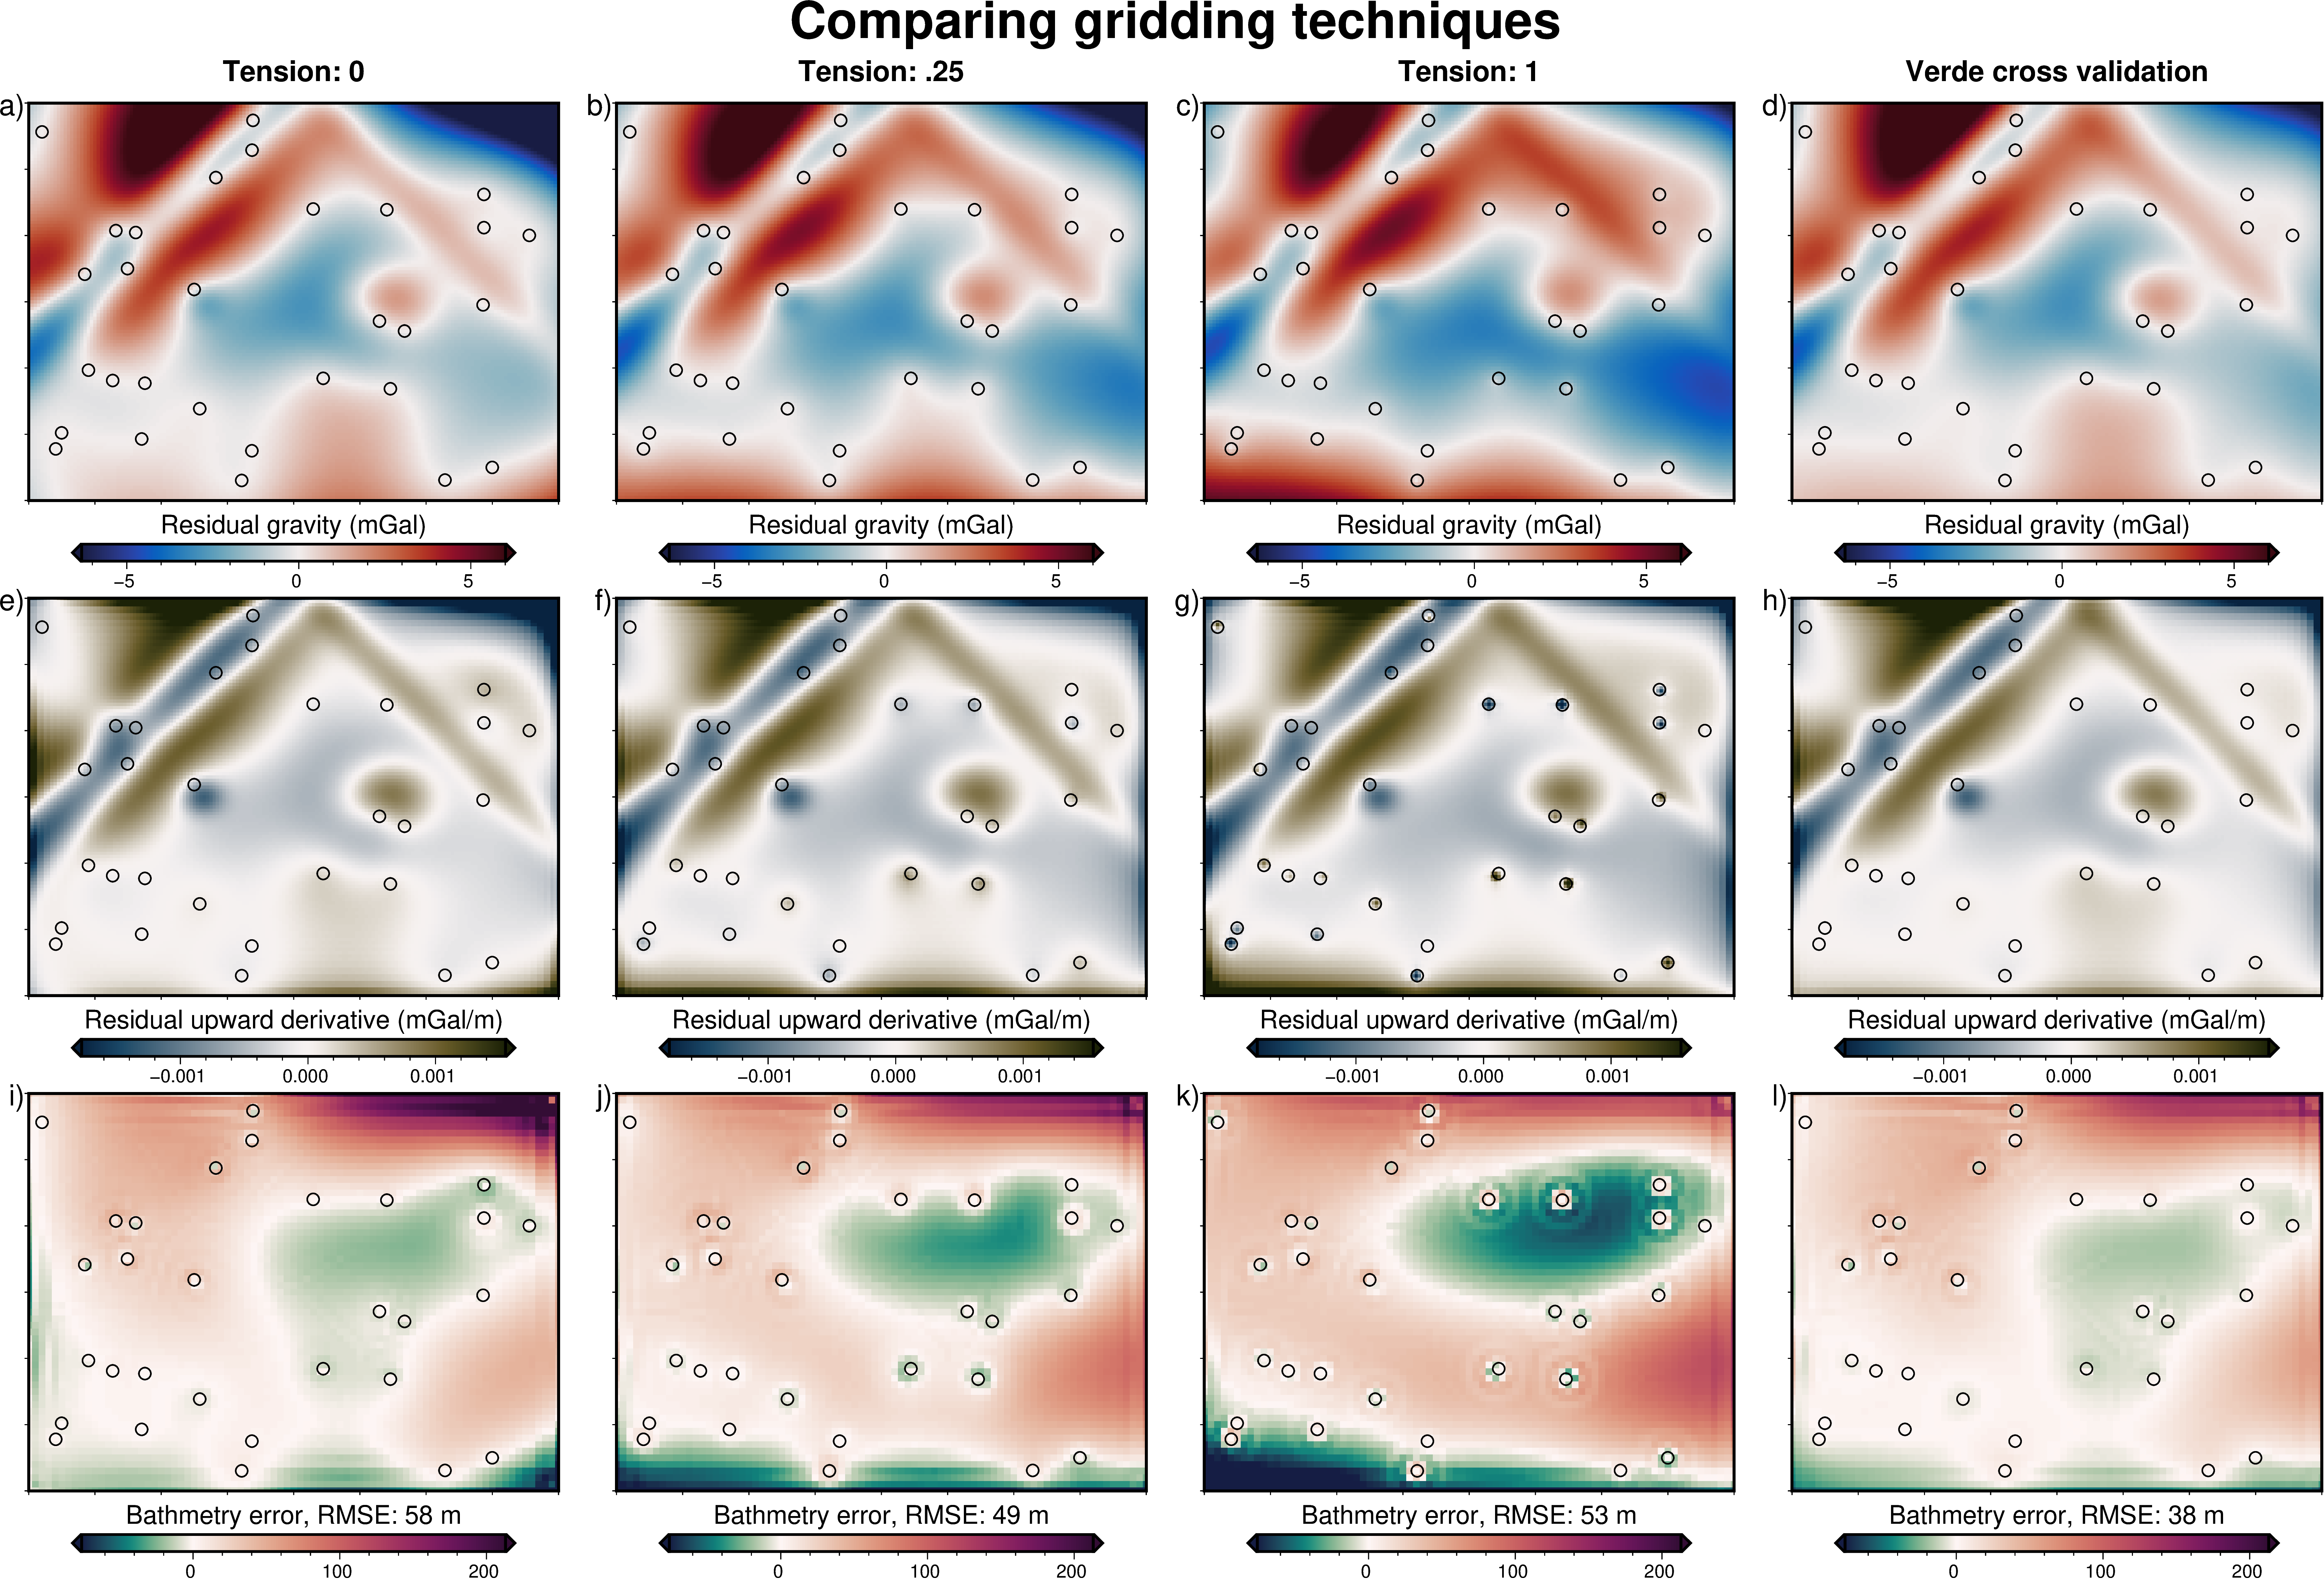
\includegraphics[width=1\textwidth]{figures/chp3/chp3_simple_regional_gridding_comparison.png}
    \caption[Constraint point minimization gridding techniques]{Comparison of gridding techniques for the constraint point minimization method of regional-residual separation. By sampling the misfit at constraints, and re-gridding over the entire domain, the regional component of the misfit is estimated. Gridding methods include minimum curvature gridding with tension factors of 0 (\textbf{column 1}), 0.25 (\textbf{column 2}), 1 (\textbf{column 3}), and cross-validated bi-harmonic spline gridding (\textbf{column 4}). Resulting gridded regional components were removed from the misfit grids to produce the residual grids (\textbf{a-d}). Second row (\textbf{e-h}) shows the vertical derivative of the residual, to highlight the gridding variations. Third row (\textbf{i-l}) shows the error of the inverted bathymetries with the true bathymetry. Constraint points are shown as open circles. Colourmaps are identical across all columns. Profiles of these data are shown in Figure \ref{fig:appB_simple_regional_gridding_comparison_profile} of Appendix \ref{appendix:B}.}
    \label{fig:chp3_simple_regional_gridding_comparison}
\end{figure}

\subsubsection{Gridding comparison}

In this section, the effect which the gridding process has on the inverted bathymetry is analyzed. Four sets of regional separations were conducted, three using the tensioned minimum curvature technique, and one using the bi-harmonic spline technique. For the three minimum curvature separations, the tension factors used were the end members, 0 and 1, and the suggested value for geopotential data, 0.25. For the bi-harmonic spline, a cross-validation with 20 varying damping values was conducted, and the best resulting damping value was used. For each of the four calculated regional fields, the resulting residual fields (Figure \ref{fig:chp3_simple_regional_gridding_comparison}a-d) were used as inputs to an inversion. All four residual anomaly data were included in an inversion damping parameter cross-validation, as described in Section \ref{chp3:simple_model_CV}. The difference between the resulting inverted bathymetry and the true bathymetry of each model is shown in Figure \ref{fig:chp3_simple_regional_gridding_comparison}i-l. To help visualize the difference in the resulting residual grids, \ref{fig:chp3_simple_regional_gridding_comparison}e-h shows the vertical derivative of the residual fields. This highlights that while the residual values at the constraints are all similar, the slope of the residual in the vicinity of the grids is strongly dependent on the gridding method \footnote{Note that the gridding process creates the regional field (not shown in Figure \ref{fig:chp3_simple_regional_gridding_comparison}), which when subtracted from the total misfit gives the residual field. The residual grid is affected by these gridding effects through the removal of the regional field.}. Additionally, the minimum curvature gridding is shown, in subplots a-c, to create large artificial anomalies away from constraint points (low values in upper right corners). These gridding artifacts result in large errors in the resulting bathymetry \ref{fig:chp3_simple_regional_gridding_comparison}i-k. The bi-harmonic spline interpolator (last column in \ref{fig:chp3_simple_regional_gridding_comparison}) is shown to produce a residual field that adheres to the constraints, has smooth curvature near constraints, and doesn't create large artificial anomalies. The effectiveness of this interpolator is confirmed by the low RMS difference between the inverted and true bathymetry (38~m). Figure \ref{fig:appB_simple_regional_gridding_comparison_profile} in Appendix \ref{appendix:B} shows a profile of the resulting regional fields and inverted bathymetries of these various gridding methods. With the bi-harmonic spline gridding techniques shown to be the most effective, the remainder of this chapter uses this gridding technique for the constraint point minimization method of regional separation.

\begin{figure}[!ht]
  \centering
    \begin{subfigure}[t]{.40\textwidth}
        \centering
        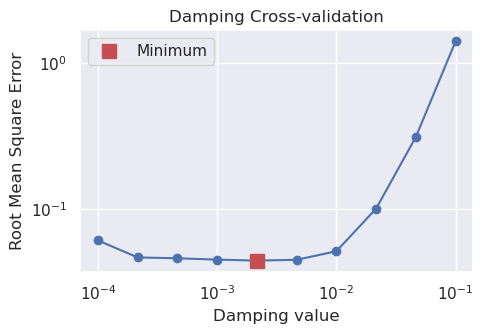
\includegraphics[width=\textwidth]{figures/chp3/chp3_simple_regional_CV.png}
        \caption{}
    \end{subfigure}
    \begin{subfigure}[t]{.58\textwidth}
        \centering
        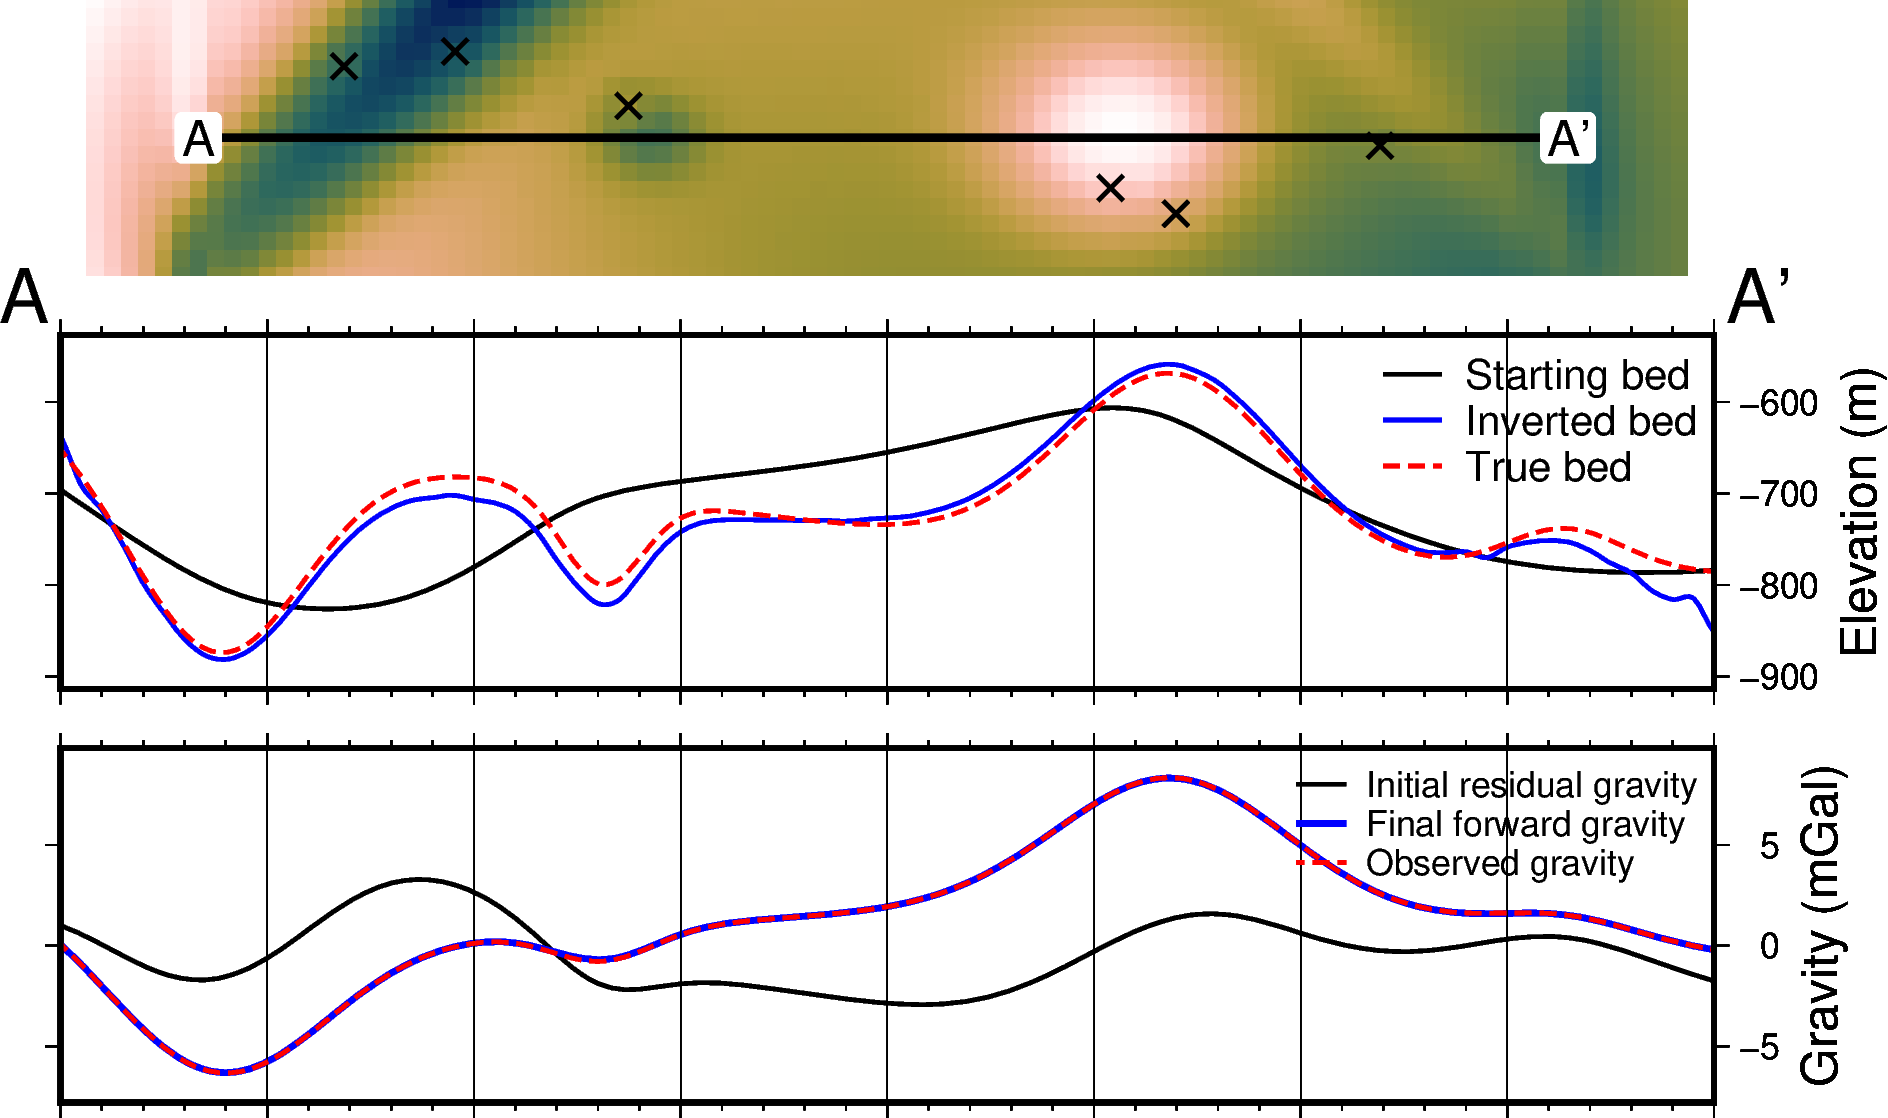
\includegraphics[width=\textwidth]{figures/chp3/chp3_simple_regional_profile.png}
        \caption{}
    \end{subfigure}
  \caption[Synthetic inversion with regional component, CV and profile]{Cross-validation and profiles for the simple synthetic inversion with a regional component removed. \textbf{a)} Cross-validation curve showing the optimal damping parameter (red square). \textbf{b)} 2D profile of the inversion results. The top panel shows profile location and constraint points (black crosses). The middle panel contains topographic profiles of the starting, inverted, and true bathymetries. The bottom panel contains gravity anomaly profiles.}
    \label{fig:chp3_simple_regional_CV_and_profile}
\end{figure}

\subsection{Inversion results}

\begin{figure}[!ht]
    \centering
    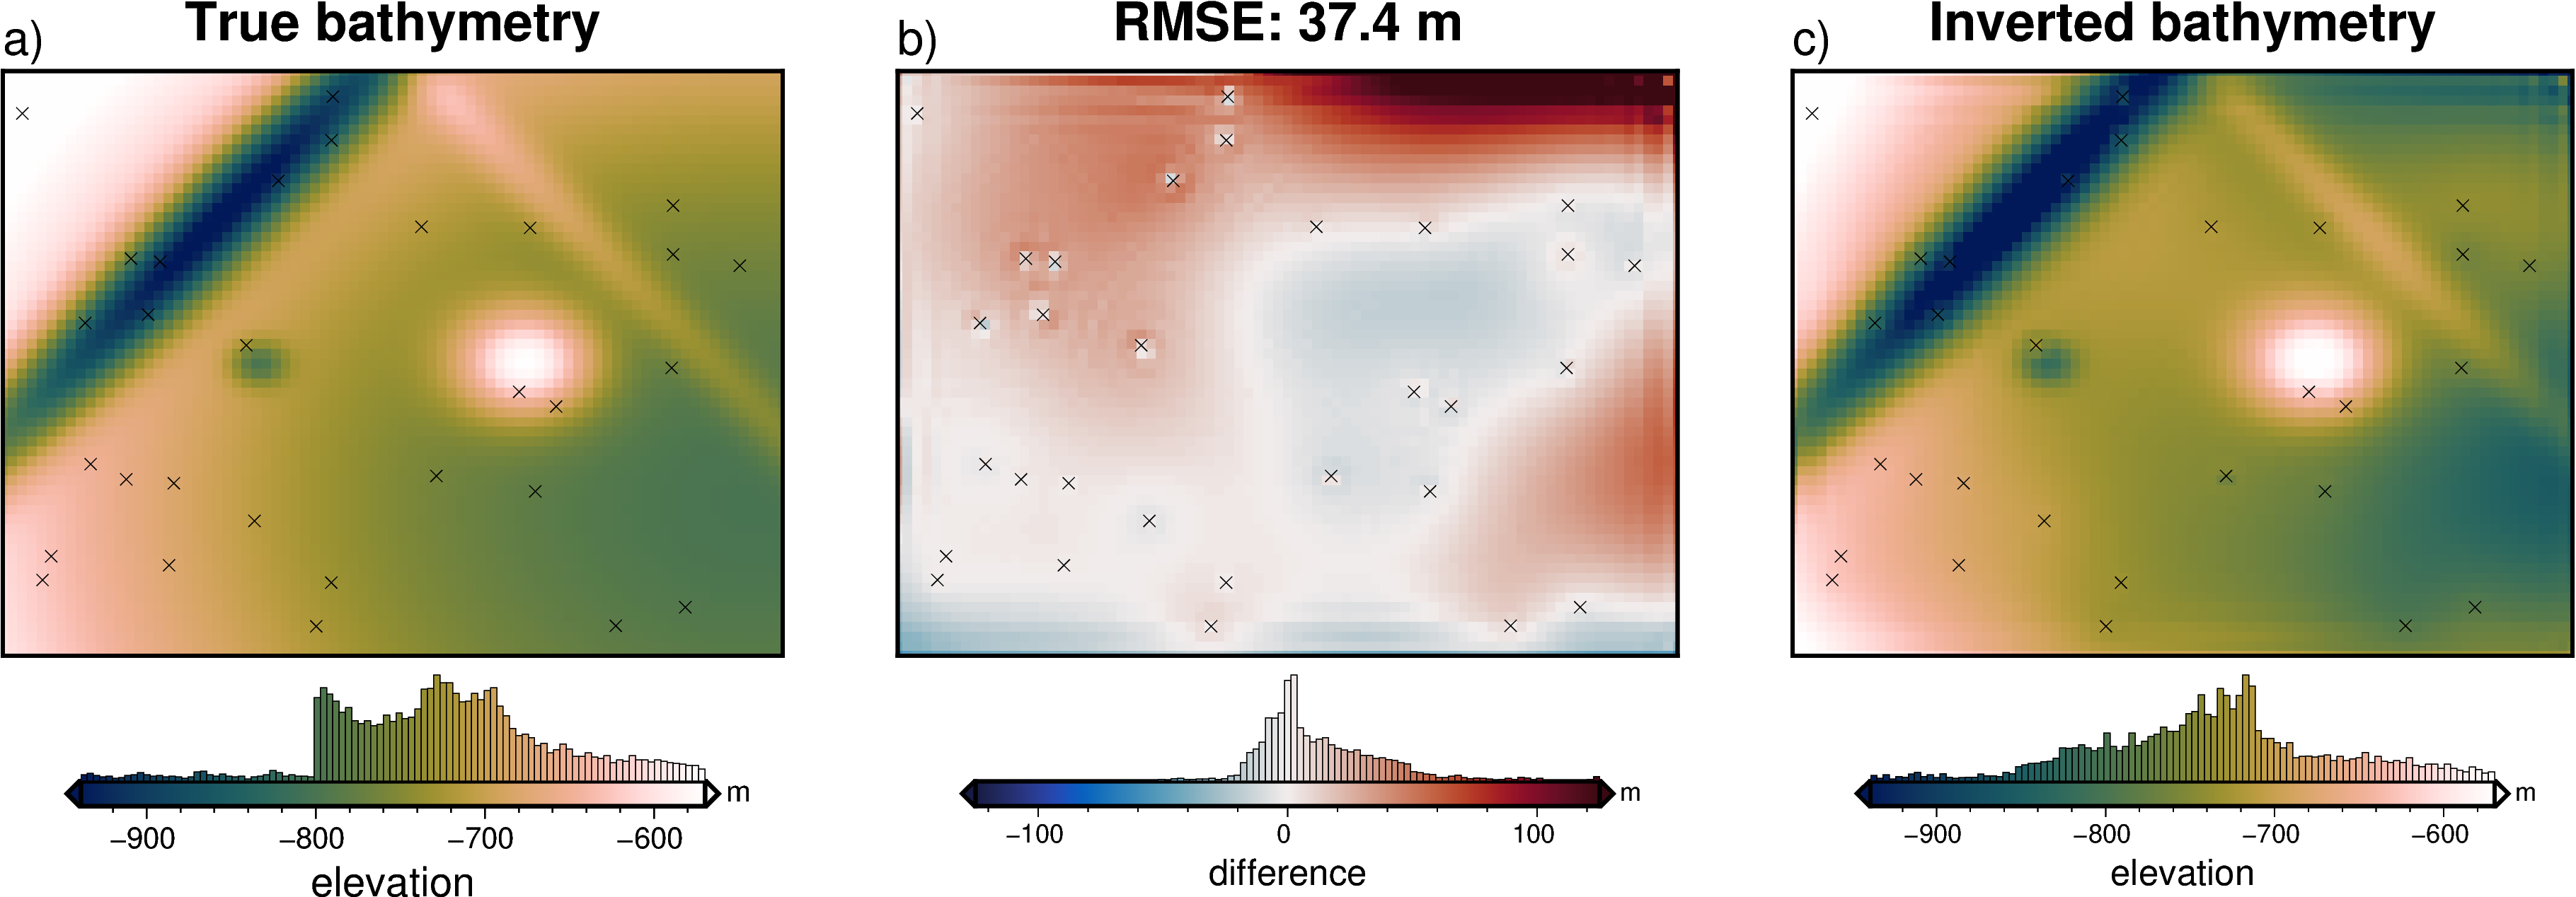
\includegraphics[width=.95\textwidth]{figures/chp3/chp3_simple_regional_results.png}
    \caption[Synthetic inversion with regional component results]{Simple synthetic model inversion with a removed regional component. \textbf{a)} True bathymetry, \textbf{b)} difference between a and c, \textbf{c)} final inverted bathymetry. Black crosses are constraint points. The RMS difference with the true bathymetry at these constraints is 2~m.}
    \label{fig:chp3_simple_regional_results}
\end{figure}

Using the cross-validated bi-harmonic gridding method to separate the regional component of the gravity misfit, the resulting residual misfit was used in an inversion. The same gravity data cross-validation method of determining the optimal damping parameter is used (Figure \ref{fig:chp3_simple_regional_CV_and_profile}). The optimal damping parameter was found to be $\sim10^{-2.6}$. The resulting inversion is shown in Figure \ref{fig:chp3_simple_regional_results}. The inverted bathymetry had an RMS difference with the true bathymetry of 37~m and an RMS difference at the constraints of 2~m. The inversion was completed in 66 seconds, with 39 iterations and a final RMS residual of 0.022~mGal. The inversion was terminated due to the $\ell^2$-norm decreasing below the set threshold of 0.15~mGal\textsuperscript{1/2}. All four bathymetric features were recovered, but a lack of constraints in a few regions (the upper-right corner) lead to a miscalculation of the regional field and a subsequent over-deepening of the bathymetry. 

The regional separation, parameter cross-validation, and inversion were repeated with additive noise and re-sampling of the gravity data to a coarser resolution (Appendix \ref{appendix:B:simple_regional_inversion}). As in section \ref{chp3:simple_ensemble}, this above workflow was also repeated for an ensemble of noise levels and gravity data grid spacings, as discussed next. 

\subsection{Ensemble of Noise and Sampling values} \label{chp3:simple_regional_ensemble}

Following the method outlined in Section \ref{chp3:simple_ensemble}, an ensemble of 100 inversions with varying levels of noise and gravity observation spacings was conducted. The noise and gravity spacing changes were applied to the original observed data, and the forward calculation of the starting model, initial misfit calculation, and regional field removal were all repeated. Each model was then inverted with a cross-validation, and the resulting RMS differences with the true bathymetry are shown in Figure \ref{fig:chp3_simple_regional_ensemble}. 

\begin{figure}[!ht]
    \centering
    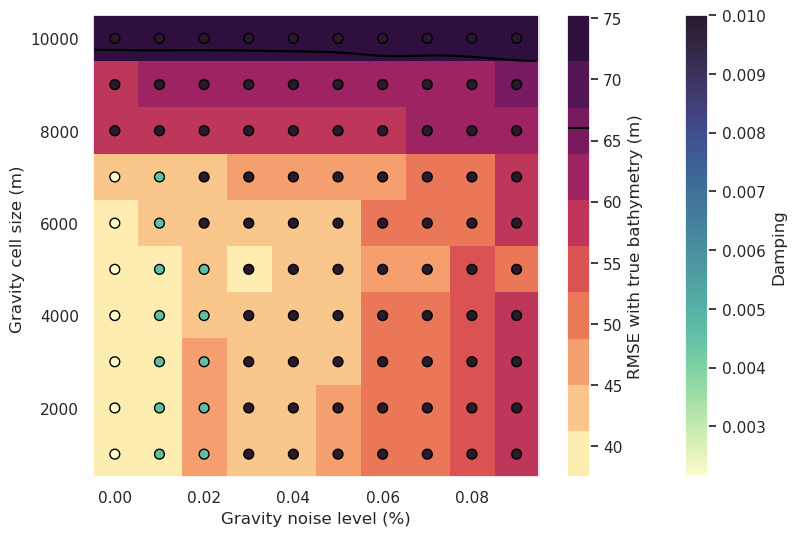
\includegraphics[width=0.9\textwidth]{figures/chp3/chp3_simple_regional_ensemble.png}
    \caption[Gravity data ensemble with regional component]{Ensemble of noise levels and gravity spacing for the simple synthetic model with a regional field. Grid cell colour indicates each inversion's RMSE with the true bathymetry. The circles' colour indicates the optimal damping value found for each inversion's cross-validation. Black line shows the 66~m contour, representing the RMS difference between the true and starting bathymetry.}
    \label{fig:chp3_simple_regional_ensemble}
\end{figure}

\subsection{Simple model comparison}

Table \ref{table:chp3_simple_synthetic_stats} compares the performance of each of the above inversions. The four inversions without a regional component of the gravity data (annulus approximation, prism approximation, with noise, and resampled), all recovered the bathymetry with an RMSE of $\sim$~10~m. With the regional component, the lowest RMS was raised to 37~m. The constraint point minimization method of regional separation produced significantly more accurate bathymetry models than the other methods. With these optimal methods and baseline performance standards, a new synthetic model is introduced which was created to emulate the expected bathymetry features and gravity anomalies associated with a sub-ice-shelf environment.

% Please add the following required packages to your document preamble:
% \usepackage{graphicx}
\begin{table}[]
\resizebox{\textwidth}{!}{%
\begin{tabular}{l|ccccc}
\multicolumn{1}{c|}{}            & \begin{tabular}[c]{@{}c@{}}RMS \\ (m)\end{tabular} & \begin{tabular}[c]{@{}c@{}}RMS at constraints \\ (m)\end{tabular} & \begin{tabular}[c]{@{}c@{}}Total time \\ (hr:min:sec)\end{tabular} & \# iterations        & \begin{tabular}[c]{@{}c@{}}Final residual RMS \\ (mGal)\end{tabular} \\ \hline
\textbf{No regional component}   & \multicolumn{1}{l}{}                               & \multicolumn{1}{l}{}                                              & \multicolumn{1}{l}{}                                               & \multicolumn{1}{l}{} & \multicolumn{1}{l}{}                                                 \\
Starting bathymetry              & 66                                                 & 0.04                                                              & –                                                                  & –                    & 2.7                                                                  \\
annulus                          & 8                                                  & 1                                                                 & 00:00:30                                                           & 37                   & 0.022                                                                \\
finite differences               & 9                                                  & 1                                                                 & 00:02:49                                                           & 37                   & 0.022                                                                \\
2\% noise                        & 12                                                 & $< 1$                                                             & 00:00:13                                                           & 18                   & 0.16                                                                 \\
6~km re-grid                     & 11                                                 & 1                                                                 & 00:00:29                                                           & 38                   & 0.019                                                                \\ \hline
\textbf{With regional component} &                                                    &                                                                   &                                                                    &                      &                                                                      \\
Starting bathymetry              & 66                                                 & 0.04                                                              & –                                                                  & –                    & 7.4                                                                  \\
filter                           & 48                                                 & –                                                                 & –                                                                  & –                    & –                                                                    \\
trend                            & 54                                                 & –                                                                 & –                                                                  & –                    & –                                                                    \\
equivalent sources               & 53                                                 & –                                                                 & –                                                                  & –                    & –                                                                    \\
constraint point minimization    & 37                                                 & 2                                                                 & 00:01:06                                                           & 39                   & 0.022                                                                \\
2\% noise                        & 45                                                 & 2                                                                 & 00:00:12                                                           & 13                   & 0.23                                                                 \\
4~km re-grid                     & 38                                                 & 2                                                                 & 00:00:51                                                           & 38                   & 0.022                                                               
\end{tabular}%
}
\caption[Simple synthetic model summary]{Summary of the simple synthetic model inversion results.}
\label{table:chp3_simple_synthetic_stats}
\end{table}



\section{Ross Sea model} \label{chp3:Ross_Sea}

Here a semi-realistic model is introduced. In the past section, two synthetic topographies (bathymetry and a crustal layer) were used in forward modelling to create synthetic gravity data. Here, real topographic data are used to create the synthetic gravity. This model is termed semi-realistic since the gravity is synthetically calculated, but it results from geologically real surfaces. This model uses data from Antarctica's Ross Sea (Figure \ref{fig:chp3_ice_shelves}, north of Ross Ice Shelf). The bathymetry data are from the IBCSO v2 data compilation \citep{dorschelinternational2022}, resampled at a 5~km resolution (Figure \ref{fig:chp3_Ross_Sea_layers_and_forwards}a). This data are mostly from shipborne multi-beam echo sounding. To create the regional component of gravity, basement depths from the ANTOSTRAT compilation of shipborne seismic data have been used \citep{brancolinidescriptive1995}, at a 5 km resolution (Figure \ref{fig:chp3_Ross_Sea_layers_and_forwards}b). The inversion domain is 320~$\times$~420~km and a buffer zone of 40~km was included in all directions, resulting in 8000 grid cells per surface. \\

\begin{figure}[!ht]
    \centering
    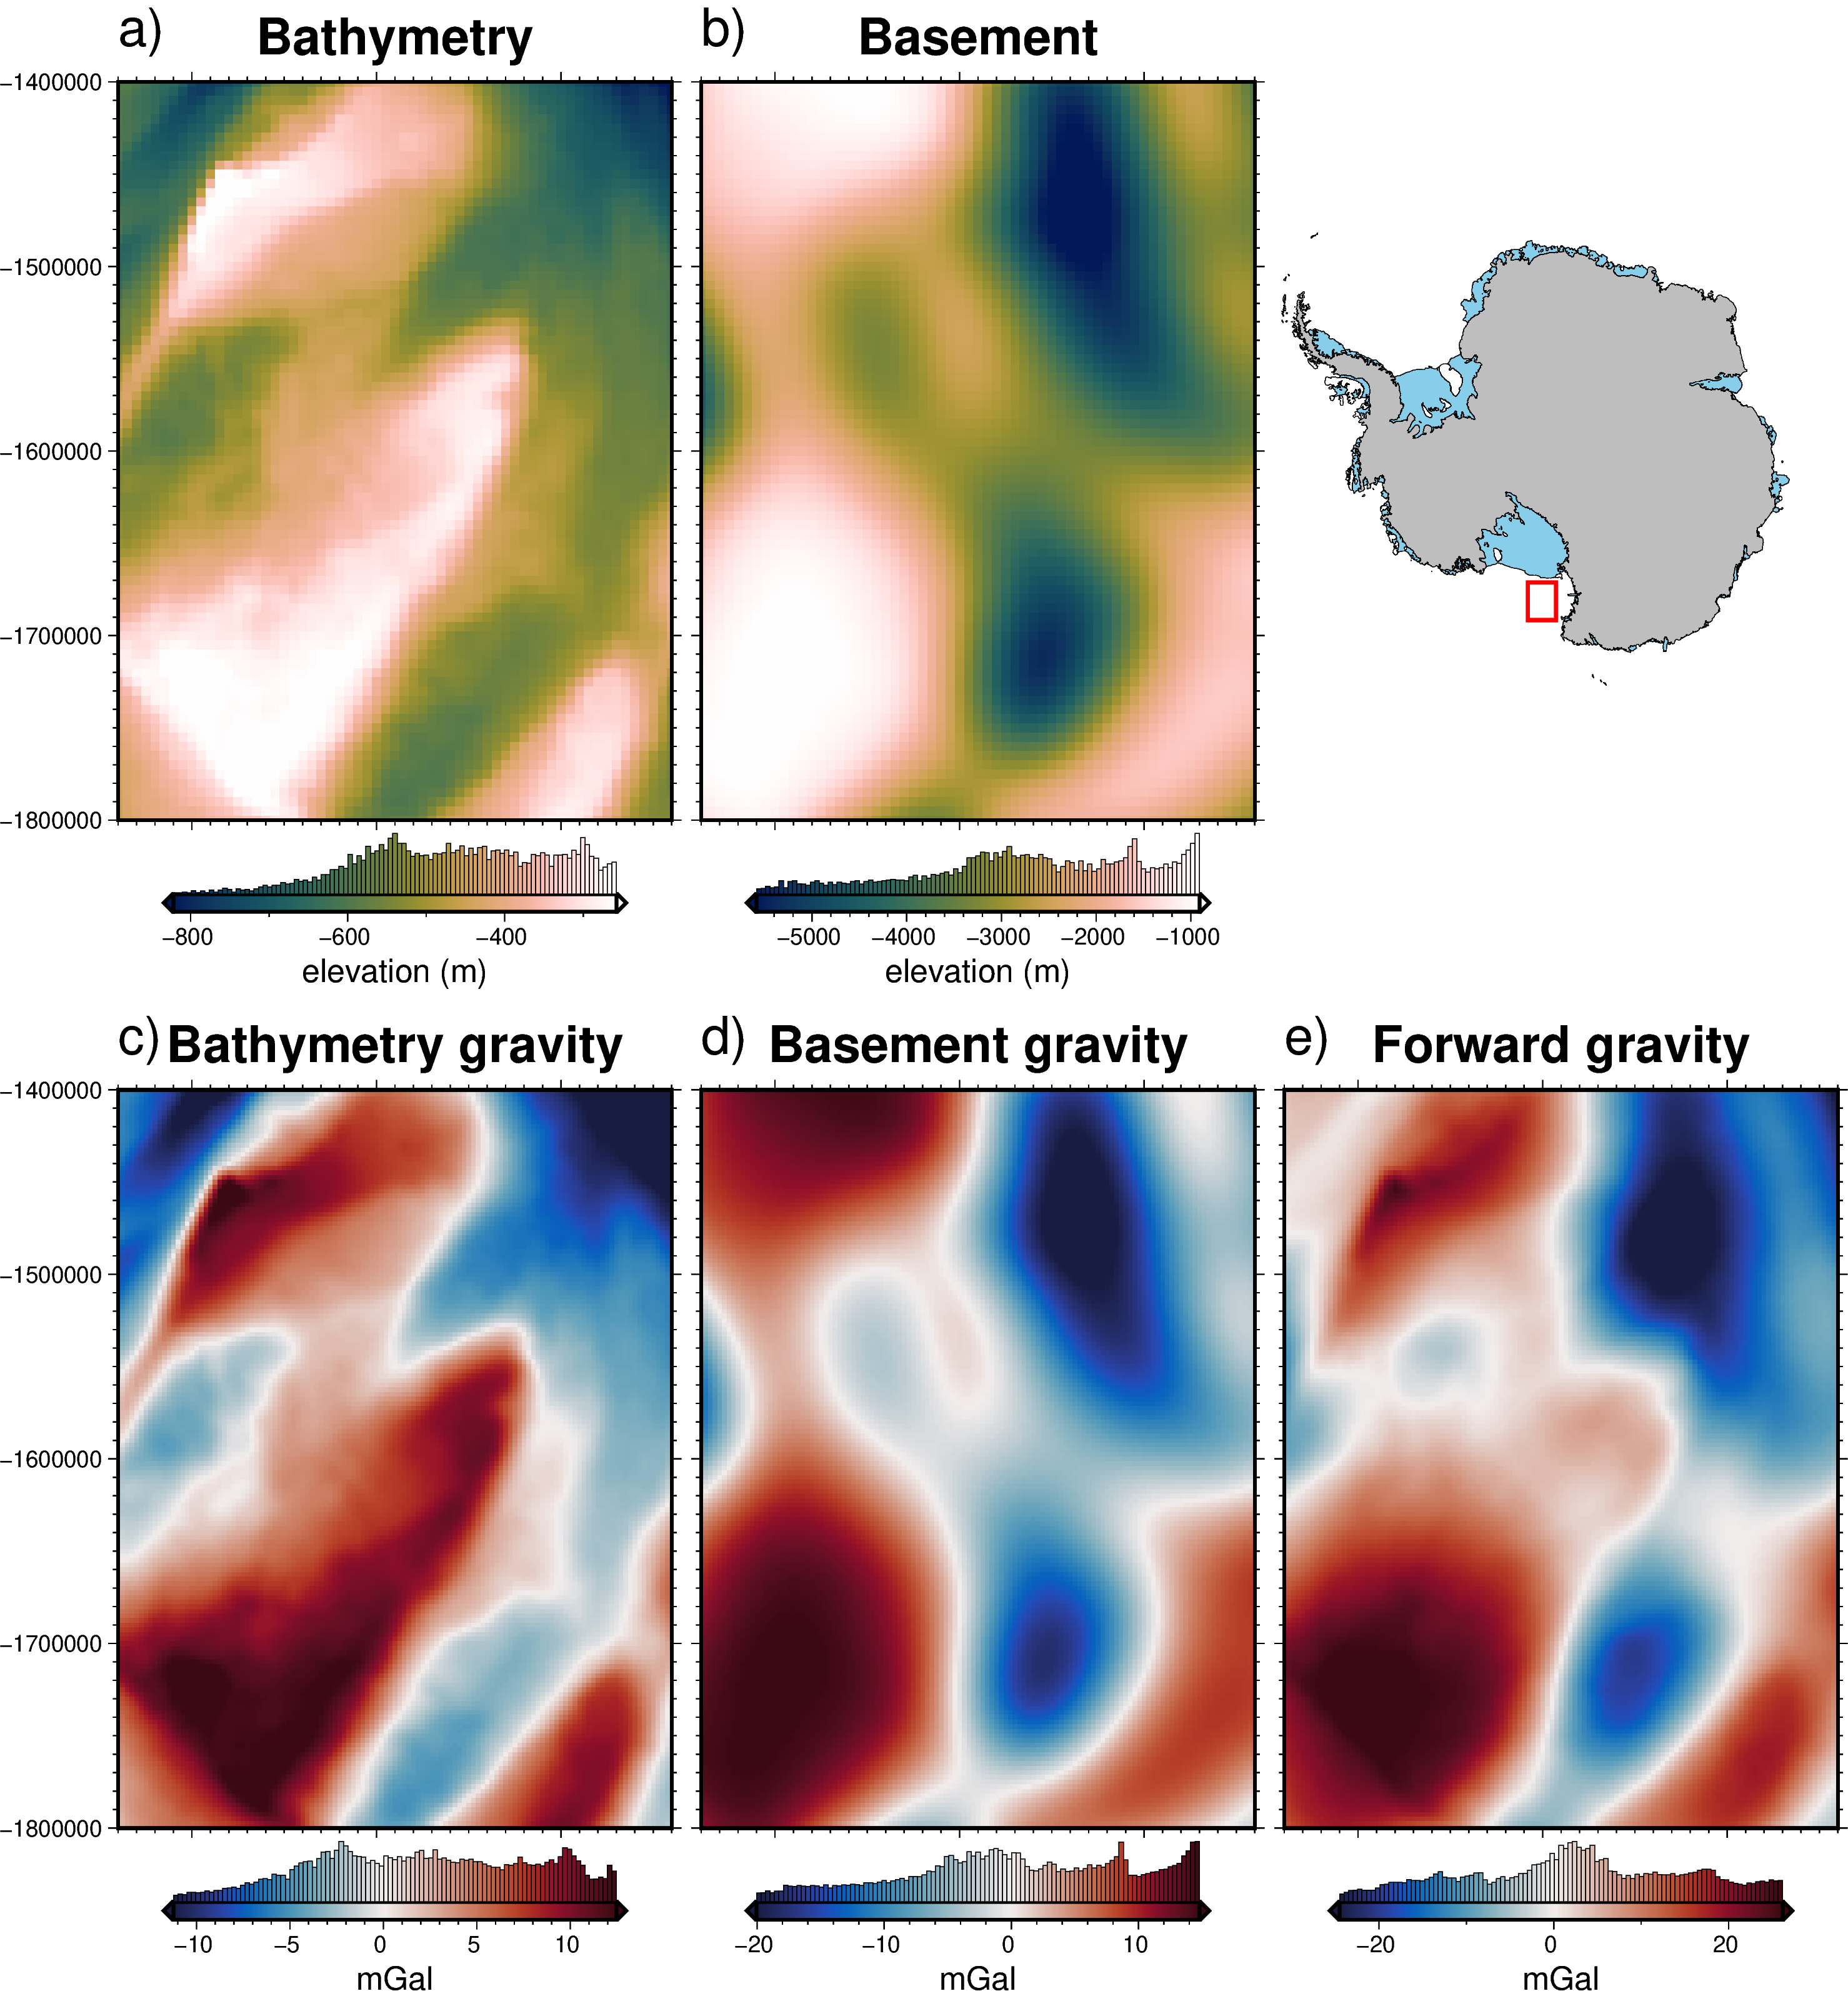
\includegraphics[width=0.95\textwidth]{chp3/chp3_Ross_Sea_layers_and_forwards.png}
    \caption[Ross Sea semi-synthetic model]{Ross Sea semi-synthetic model. \textbf{a)} Bathymetry data at 5~km resolution from IBCSO v2 \citep{dorschelinternational2022}, \textbf{b)} basement topography from the ANTOSTRAT project at 5~km resolution \citep{brancolinidescriptive1995}, \textbf{c)} forward gravity calculated at a regular 5~km grid at 1~km altitude for the bathymetry and \textbf{d)} for the basement. \textbf{e)} Total forward gravity from the combinations of c and d. Location of Ross Sea inversion domain shown as red box.}
    \label{fig:chp3_Ross_Sea_layers_and_forwards}
\end{figure}

\subsection{Observed gravity}

The bathymetric and crustal surfaces were discretized with the reference discretization method (Figure \ref{fig:chp3_discretization}e) with the mean elevation of each surface as its reference level. A density contrast of $\Delta\rho$ = 1276~kg~m\textsuperscript{-1} (contrast between seawater(1024~kg~m\textsuperscript{-1}) and sediment (2300~kg~m\textsuperscript{-1})), was used, with $+\Delta\rho$ for prisms above the reference, and $-\Delta\rho$ for prisms below the reference. For the basement, a density contrast of $\Delta\rho$ = 200~kg~m\textsuperscript{-1} was used, representing the contrast between sediment (2300~kg~m\textsuperscript{-1}) and low-density basement rock (2500~kg~m\textsuperscript{-1}). This contrast was set so that the resulting forward gravity of the basement was slightly greater in magnitude than that of the bathymetry. The forward gravity of each layer was calculated at a regular grid of observation points with a 5 km spacing, at a constant elevation of 1~km (Figure \ref{fig:chp3_Ross_Sea_layers_and_forwards}c-d). This created the full-resolution synthetic observed gravity dataset. To represent an airborne gravity survey, this grid is sampled along synthetic flight lines. \\

This synthetic survey (Figure \ref{fig:chp3_Ross_Sea_survey}b) consisted of five N-S and 24 E-W flight lines. Spacing between lines was 50~km for the N-S lines and 15~km for the E-W lines. One N-S line and 3 E-W were omitted to represent missed flights. Along line spacing of data was 5~km. This survey configuration is similar to other Antarctic airborne surveys \citep{tintoross2019}. The full resolution gravity (Figure \ref{fig:chp3_Ross_Sea_survey}a) was sampled at these flight line locations, and the resulting values were fitted with equivalent sources. Gravity observations were then predicted from these sources on an even 5~km grid\footnote{The gravity observations were actually interpolated onto a 2.5~km grid to account for the testing data.} over the whole domain (Figure \ref{fig:chp3_Ross_Sea_survey}c). Lastly, the survey data were contaminated with noise from a Gaussian distribution, with a mean of 0 and a standard deviation of 0.6~mGal (2\% of the max absolute value of the full-resolution data). The difference between the true gravity and this noise-contaminated synthetic survey (Figure \ref{fig:chp3_Ross_Sea_survey}b) represents the typical loss of data resulting from a sparse airborne survey. The RMS difference is 0.75~mGal. The largest differences are located within the flight line data gaps. \\

\begin{figure}[!ht]
    \centering
    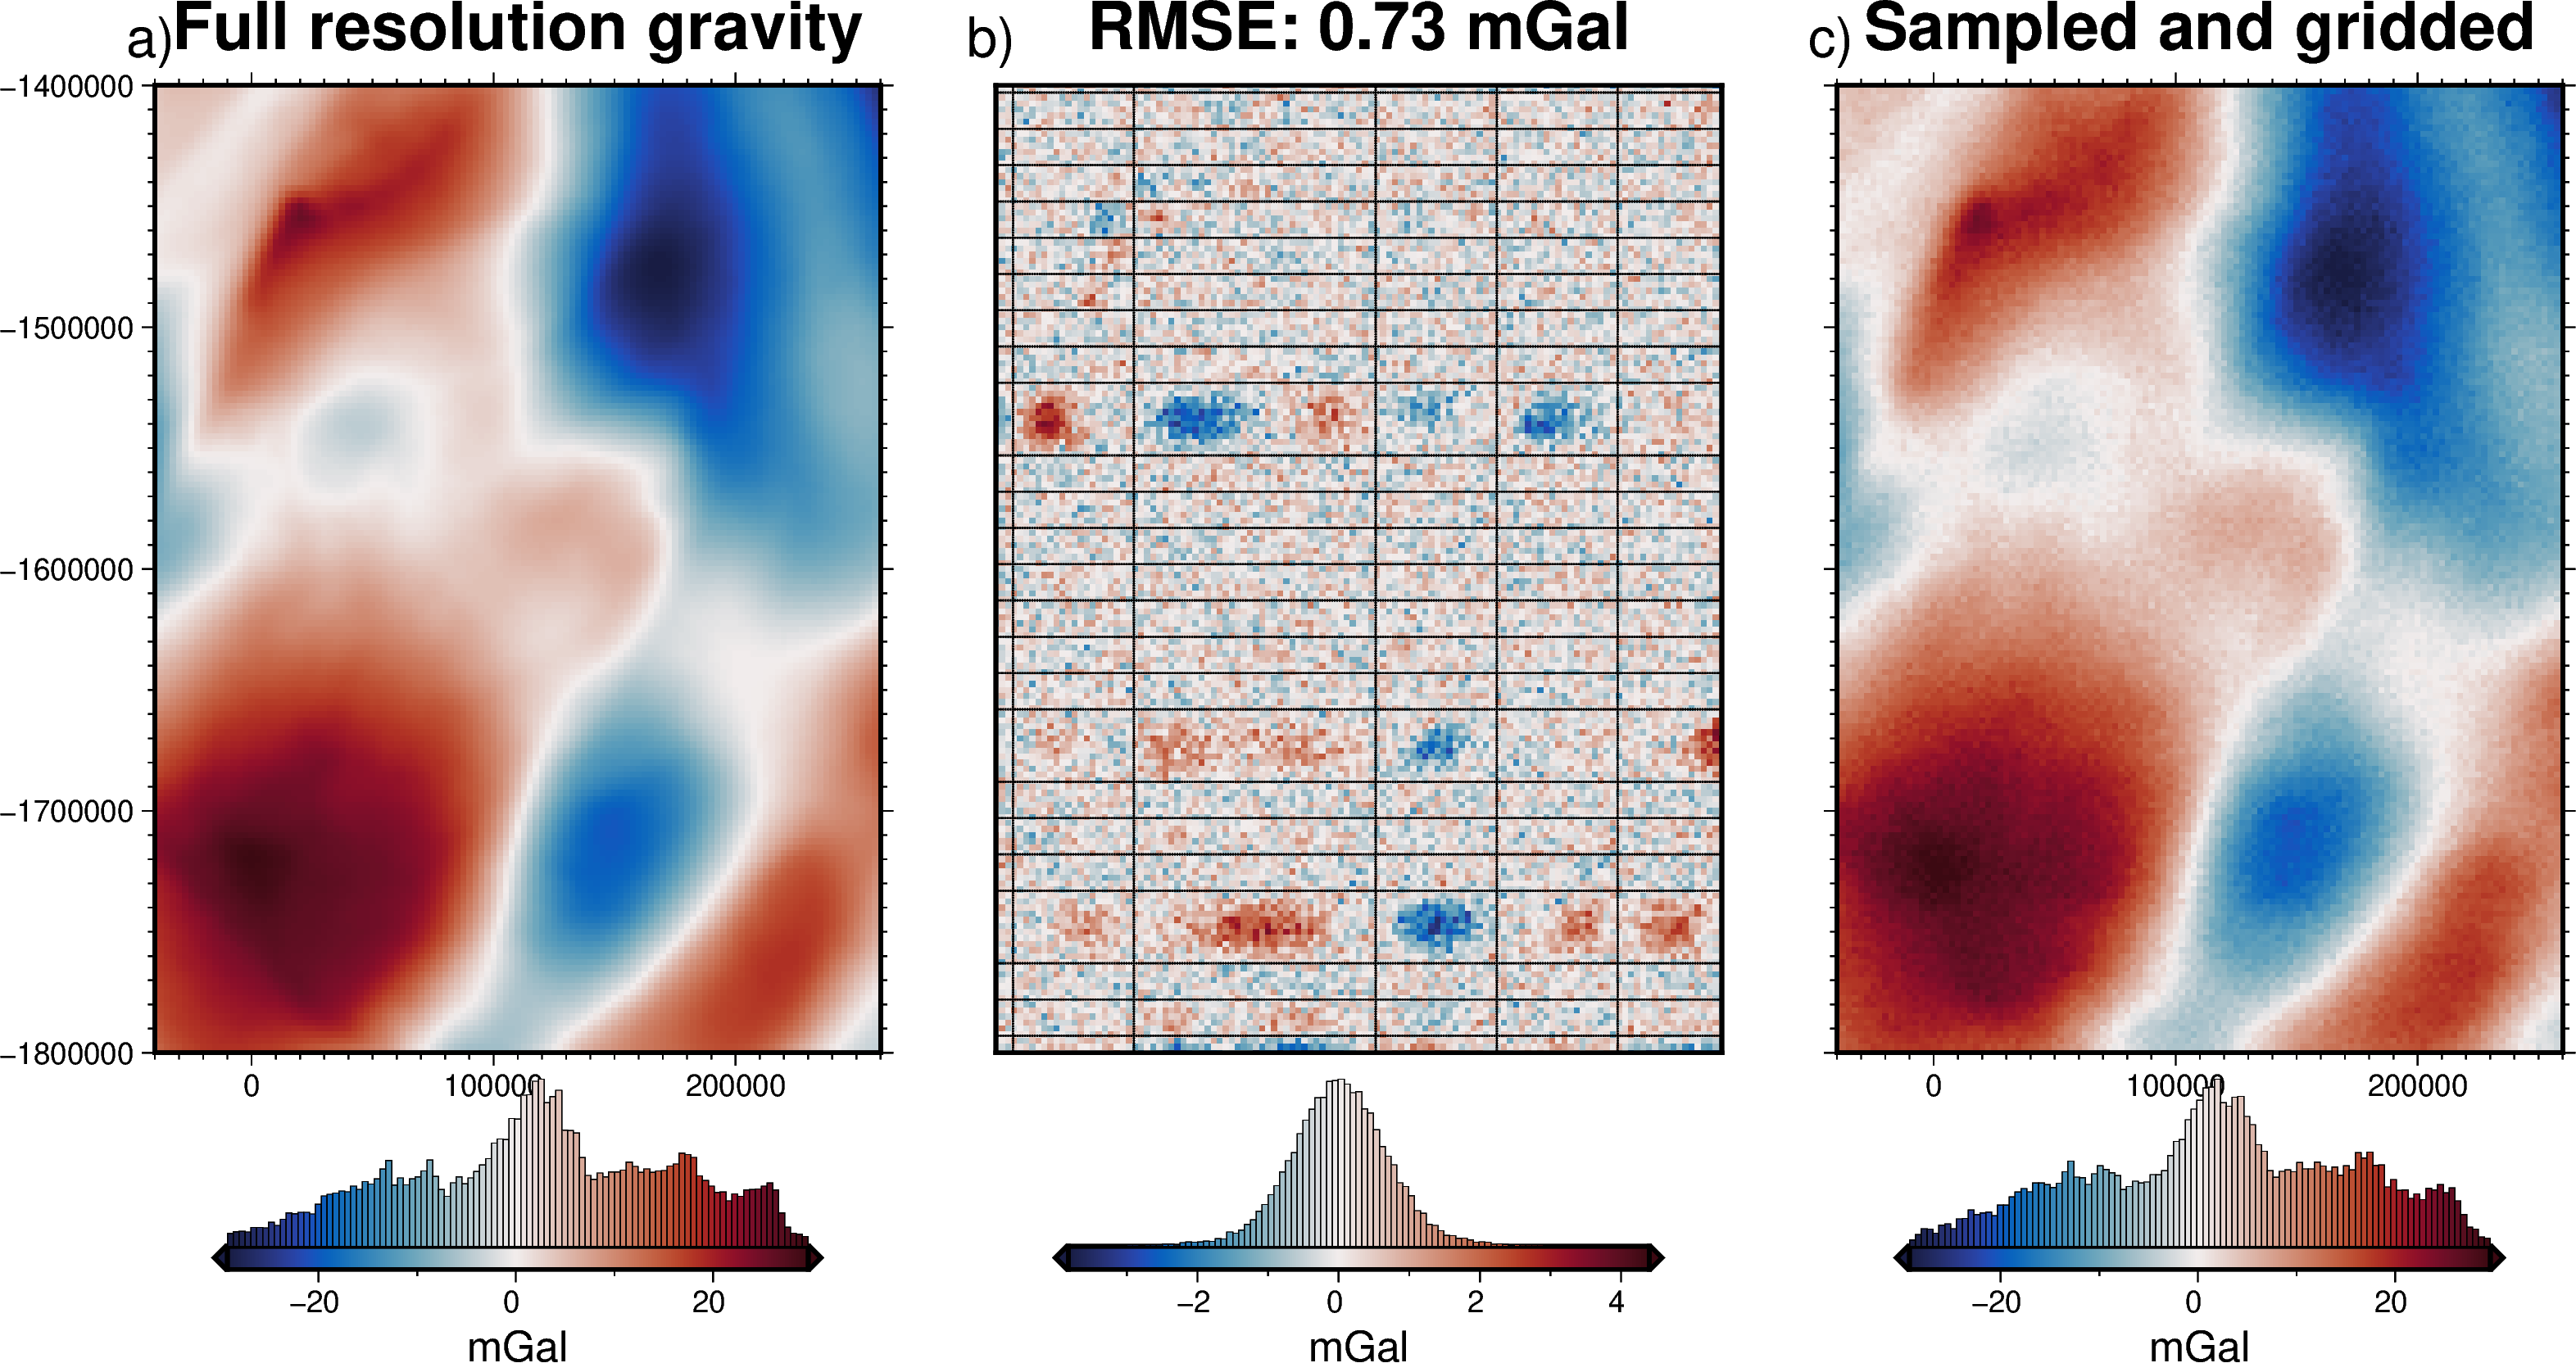
\includegraphics[width=0.8\textwidth]{figures/chp3/chp3_Ross_Sea_survey.png}
    \caption[Ross Sea synthetic airborne survey]{Ross Sea synthetic airborne survey. \textbf{a)} Full-resolution gravity data from the forward calculation of the bathymetry and basement. \textbf{b)} Difference between a and b, with black lines showing the synthetic airborne survey points. \textbf{c)} Gravity data from sampling along flight lines and re-gridded with equivalent sources.}
    \label{fig:chp3_Ross_Sea_survey}
\end{figure}

\subsection{Starting bathymetry}

The bed elevations around the borders of ice shelves are generally well-constrained. Bathymetry depths from the open ocean portion of the ice shelf border can be found through satellite altimetry or multi-beam sonar surveys. The remainder of the ice shelf border consists of grounded ice. Bed elevations beneath grounded ice can be efficiently imaged or modelled with methods such as airborne radar or mass-conservation modelling \citep{morlighemdeep2020}. Many Antarctic ice shelves also contain sparse direct measurements of bathymetry from seismic surveying. This resulting configuration for many ice shelves is generalized by a very well-constrained border with sparse constraints located within. Here, this configuration is mimicked for a hypothetical ice shelf in the Ross Sea. \\

Within the model domain, a polygon is created to represent the ice shelf border (Figure \ref{fig:chp3_Ross_Sea_starting_model}). Outside this border, constraint points are placed in each grid cell of the model ($N = 3503$, small black dots in Figure \ref{fig:chp3_Ross_Sea_starting_model}). Within the border, constraints are placed on a semi-regular grid. To represent a spatial constraint density similar to other Antarctic ice shelves\footnote{The Ross Ice Shelf has $\sim$1 constraint per 2200~km\textsuperscript{2}}, 1 constraint per 2500~km\textsuperscript{2} is used. This equates to 39 constraints. In the previous models, the true bathymetry was sampled at the constraints and the resulting values were gridded for the entire domain. Here, to represent measurement uncertainties for attaining the constraint point depths, after each point is sampled, Gaussian noise is added to the values before gridding. \\

\begin{figure}[!ht]
    \centering
    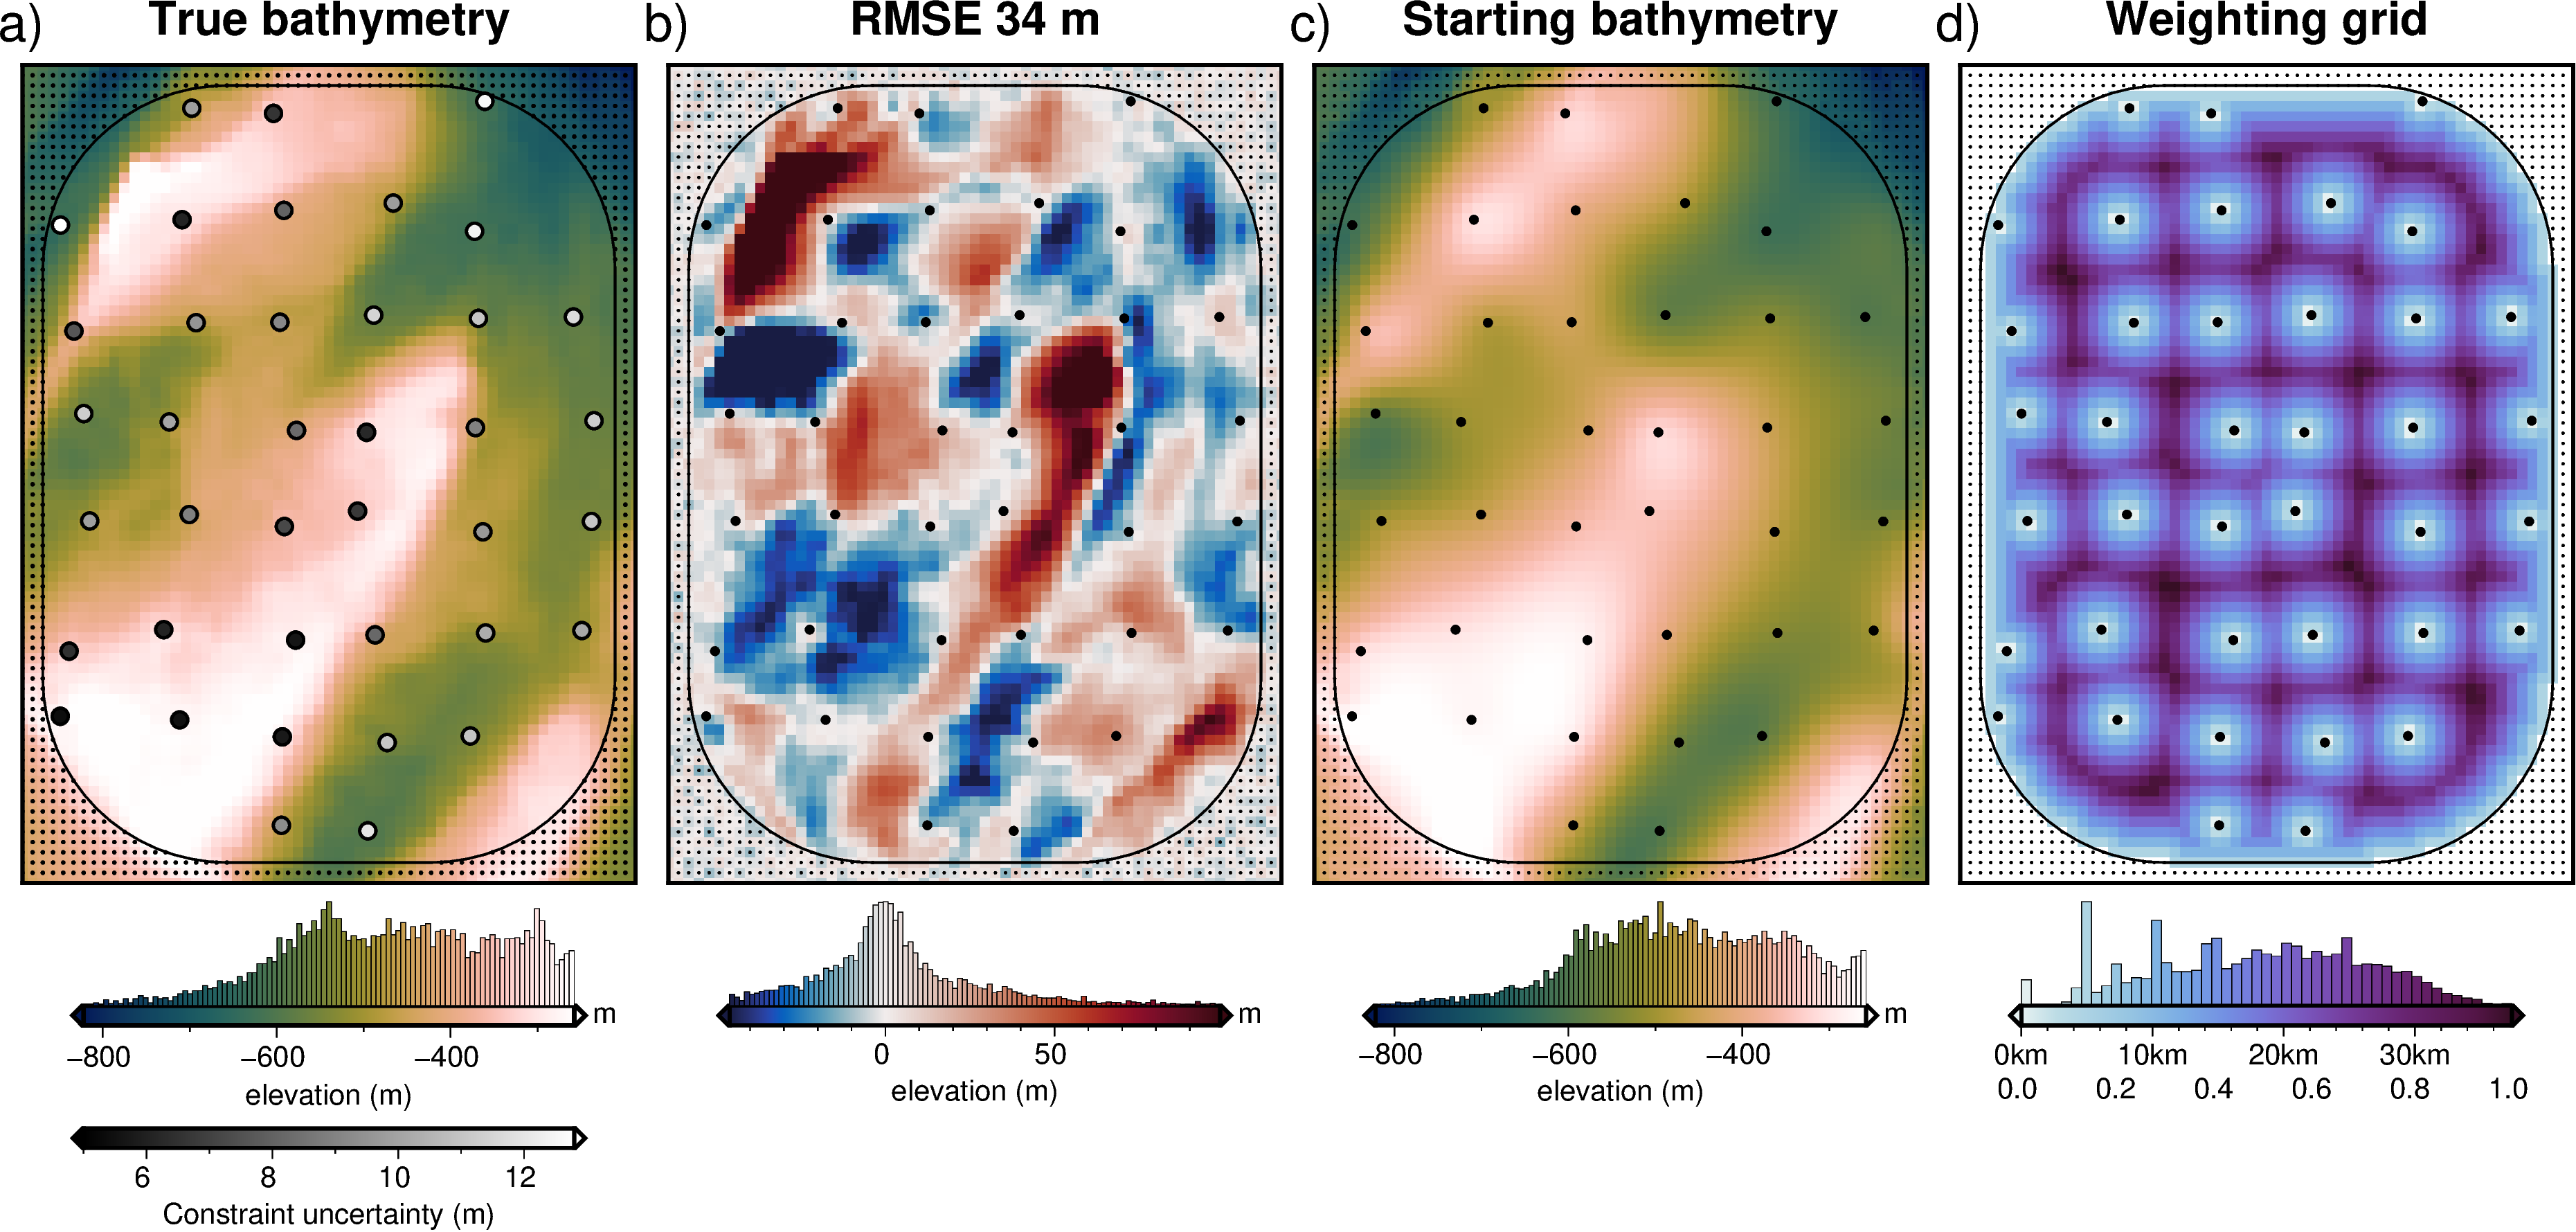
\includegraphics[width=0.95\textwidth]{figures/chp3/chp3_Ross_Sea_starting_model_semiregular.png}
    \caption[Ross Sea starting bathymetry]{Gridding of the Ross Sea starting bathymetry. \textbf{a)} True bathymetry at 5~km resolution from the IBCSO v2 compilation \citep{dorschelinternational2022}. Constraint points (coloured dots), show the uncertainty values of each point. These uncertainties were used as the standard deviations of the Gaussian function for contaminating the sampled data with noise before re-gridding. \textbf{b)} Difference between a and b, \textbf{c)} starting bathymetry from the sampling and gridding of the constraint points with added noise. \textbf{d)} Weighting grid used in the inversion. Grid colours show both the distance between each grid cell and the nearest constraint point and the weight values (0 - 1) from the normalization of these distances. Small black dots and large black dots indicate constraints outside and inside of the ice shelf border, respectively. Semi-rounded black line shows the outline of the synthetic ice shelf.}
    \label{fig:chp3_Ross_Sea_starting_model}
\end{figure}

Points outside of the ice shelf are contaminated with noise from a Gaussian distribution with a standard deviation of 5~m. This represents the well-constrained methods associated with bed observations on either grounded ice or in the open ocean. Points within the shelf are contaminated with noise based on their depth. The Gaussian distribution used has a standard deviation of 2\% of each point's depth. This simulates increasing measurement uncertainty with depth. \citet{brisbourneupdated2020} provide depth uncertainties for seismically imaged bathymetry beneath the Larsen C ice shelf, which have an average uncertainty as the percentage of depth from the surface of $\sim$2~\%. For our points, this equates to an RMS noise value of $\sim$~10 m for the ice shelf constraints. The uncertainty (the standard deviation of the Gaussian function used, not the actual value of the noise) of each point is shown in Figure \ref{fig:chp3_Ross_Sea_starting_model}a. This noise-contaminated sparse data is then gridded with a cross-validated bi-harmonic spline yielding the starting bathymetry. This interpolator takes the uncertainties of each point into account so that highly uncertain points don't introduce a bias into the interpolation \citep{uiedaverde2018}. The difference between the true and starting bathymetries had an RMS of 34~m over the whole grid, and an RMS at the constraint points of 10~m.

\subsection{Gravity misfit}

The starting bathymetry was discretized and forward modelled at the observation points with a density contrast of 1276~kg~m\textsuperscript{-1}. This forward gravity was then subtracted from the observed gravity to get the gravity misfit (Figure \ref{fig:chp3_Ross_Sea_misfit}a). Using the constraint point minimization method, the regional field was estimated with a bi-harmonic spline interpolator (Figure \ref{fig:chp3_Ross_Sea_misfit}b), which was subsequently removed, leaving the residual misfit (Figure \ref{fig:chp3_Ross_Sea_misfit}c). As in the above section, the interpolator takes the uncertainty of each constraint point into account to avoid overfitting the regional field to highly-uncertain constraint points. \\

% \begin{figure}[h]
%     \centering
%     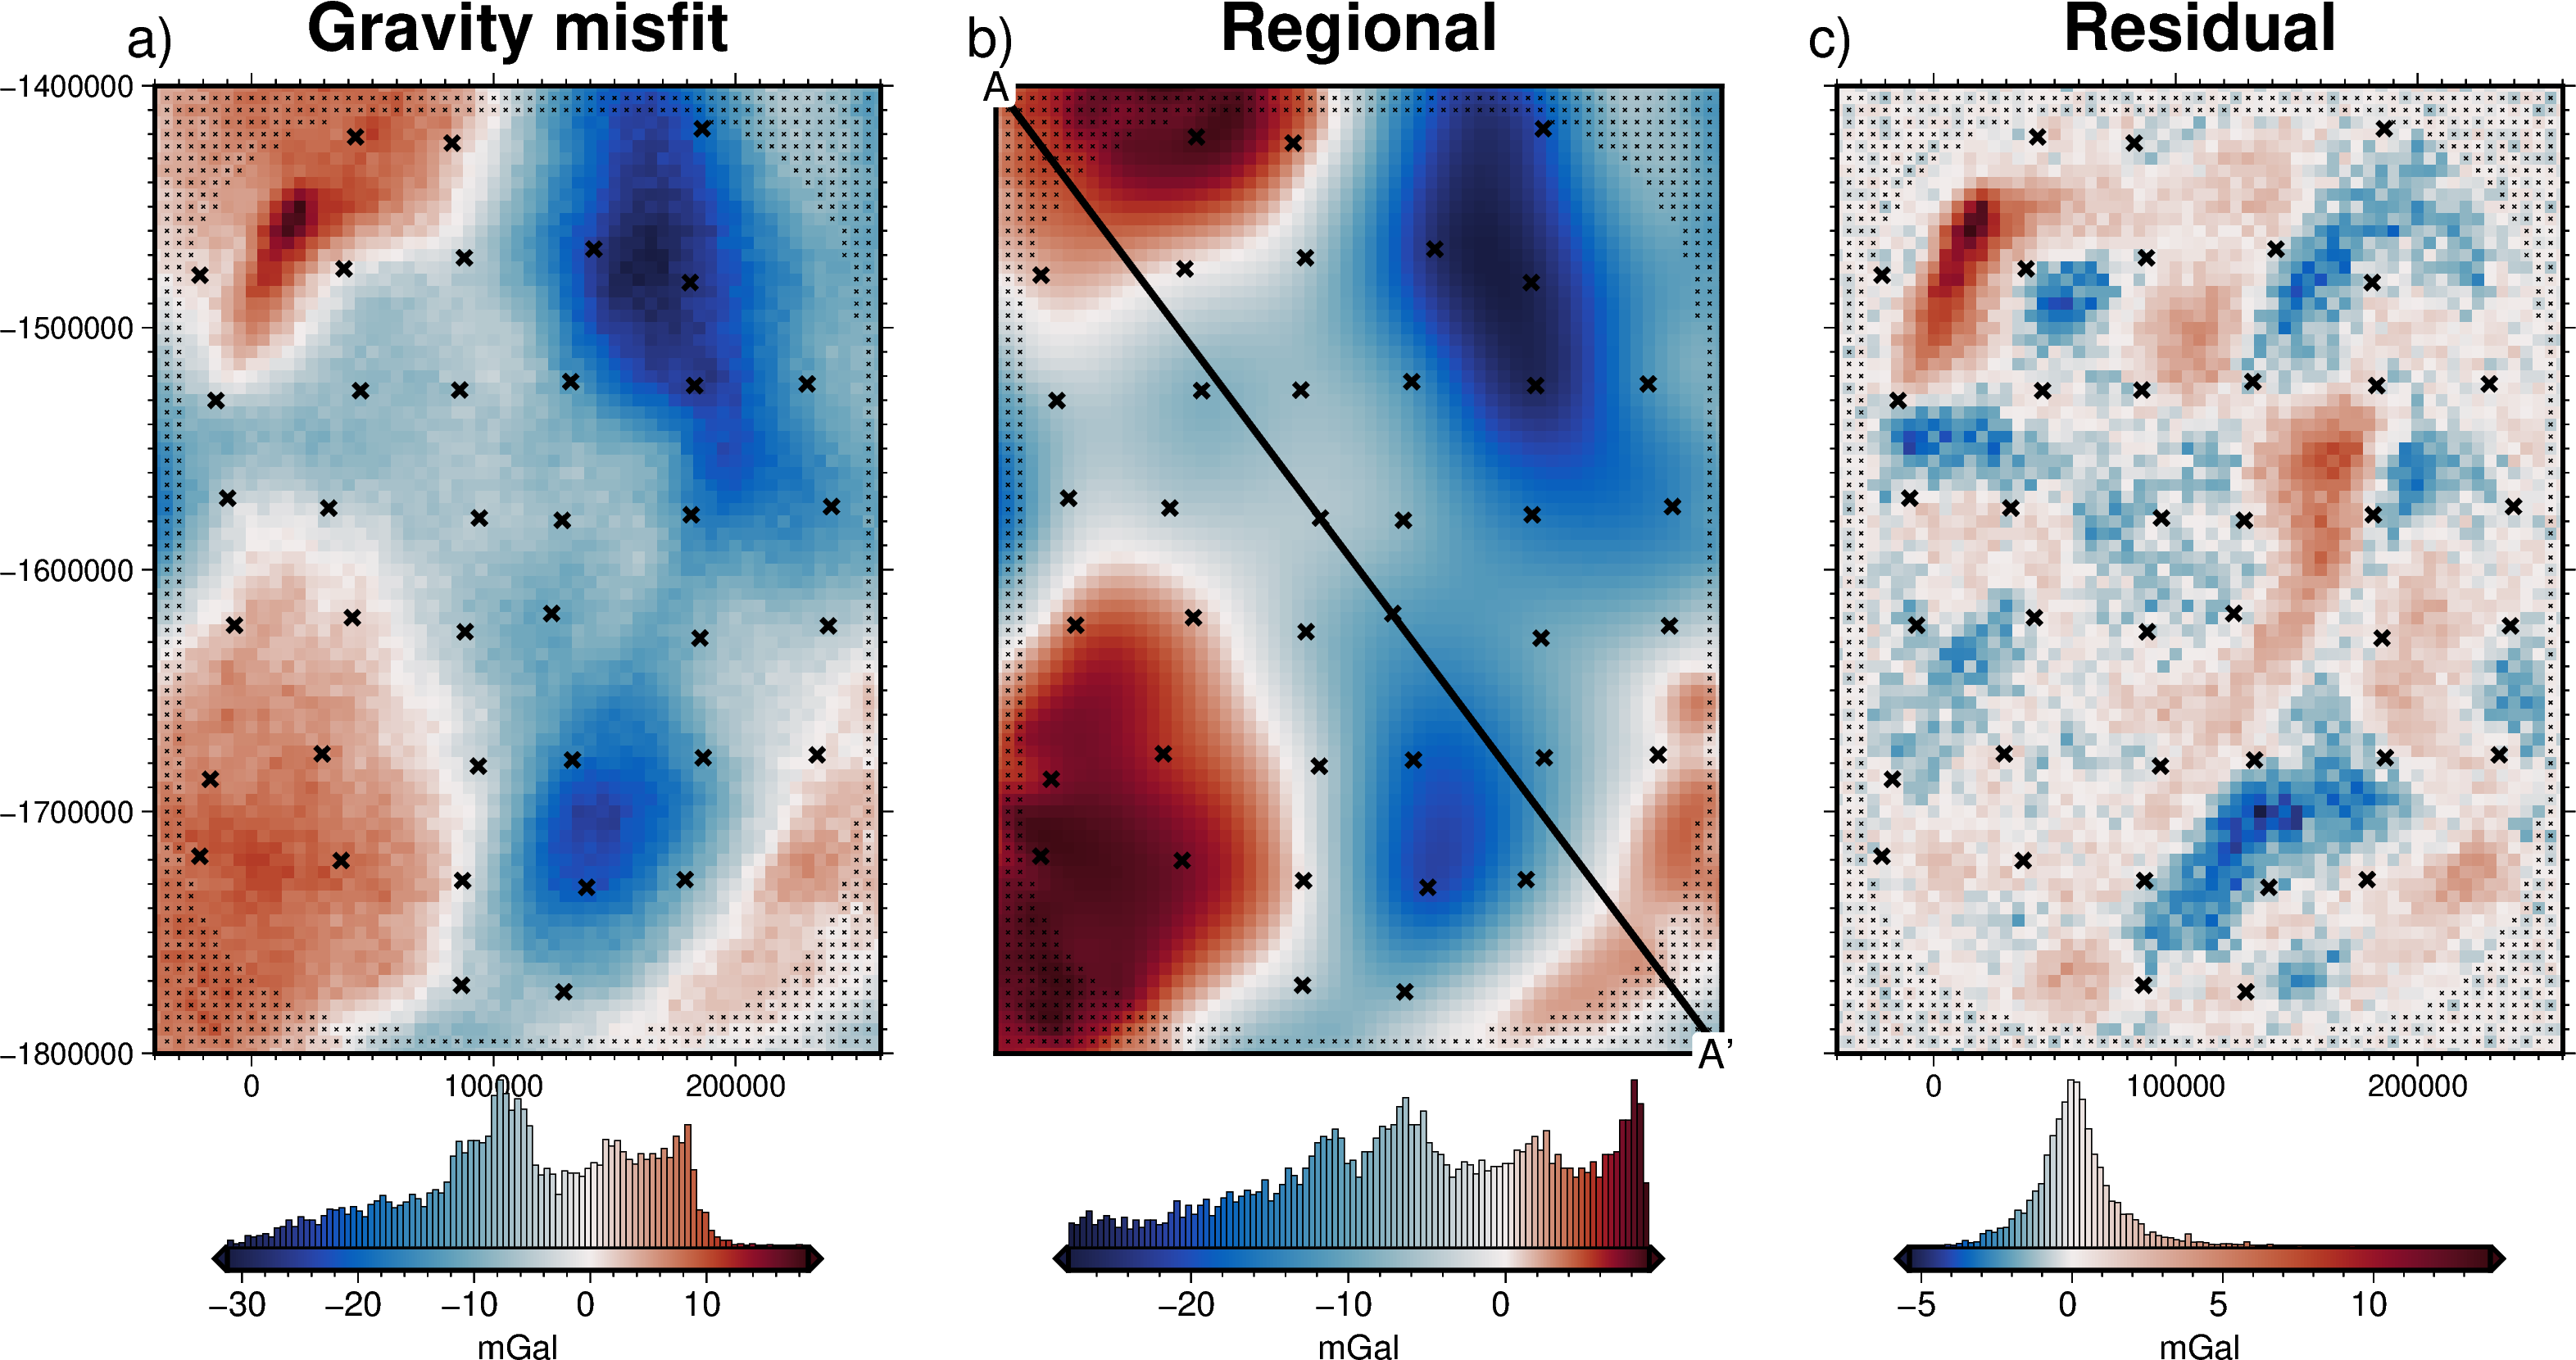
\includegraphics[width=0.95\textwidth]{figures/chp3/chp3_Ross_Sea_misfit.png}
%     \caption{Ross Sea synthetic gravity anomalies, \textbf{a)} total gravity misfit, \textbf{b)} the estimated regional component using the constraint point minimization method, and \textbf{c)}, the residual misfit, as the difference between the total misfit and the regional component. Black crosses, large and small, show constraints inside and outside the ice shelf, respectively.}
%     \label{fig:chp3_Ross_Sea_misfit}
% \end{figure}

\begin{figure}[!ht]
  \centering
    \begin{subfigure}[t]{.95\textwidth}
        \centering
        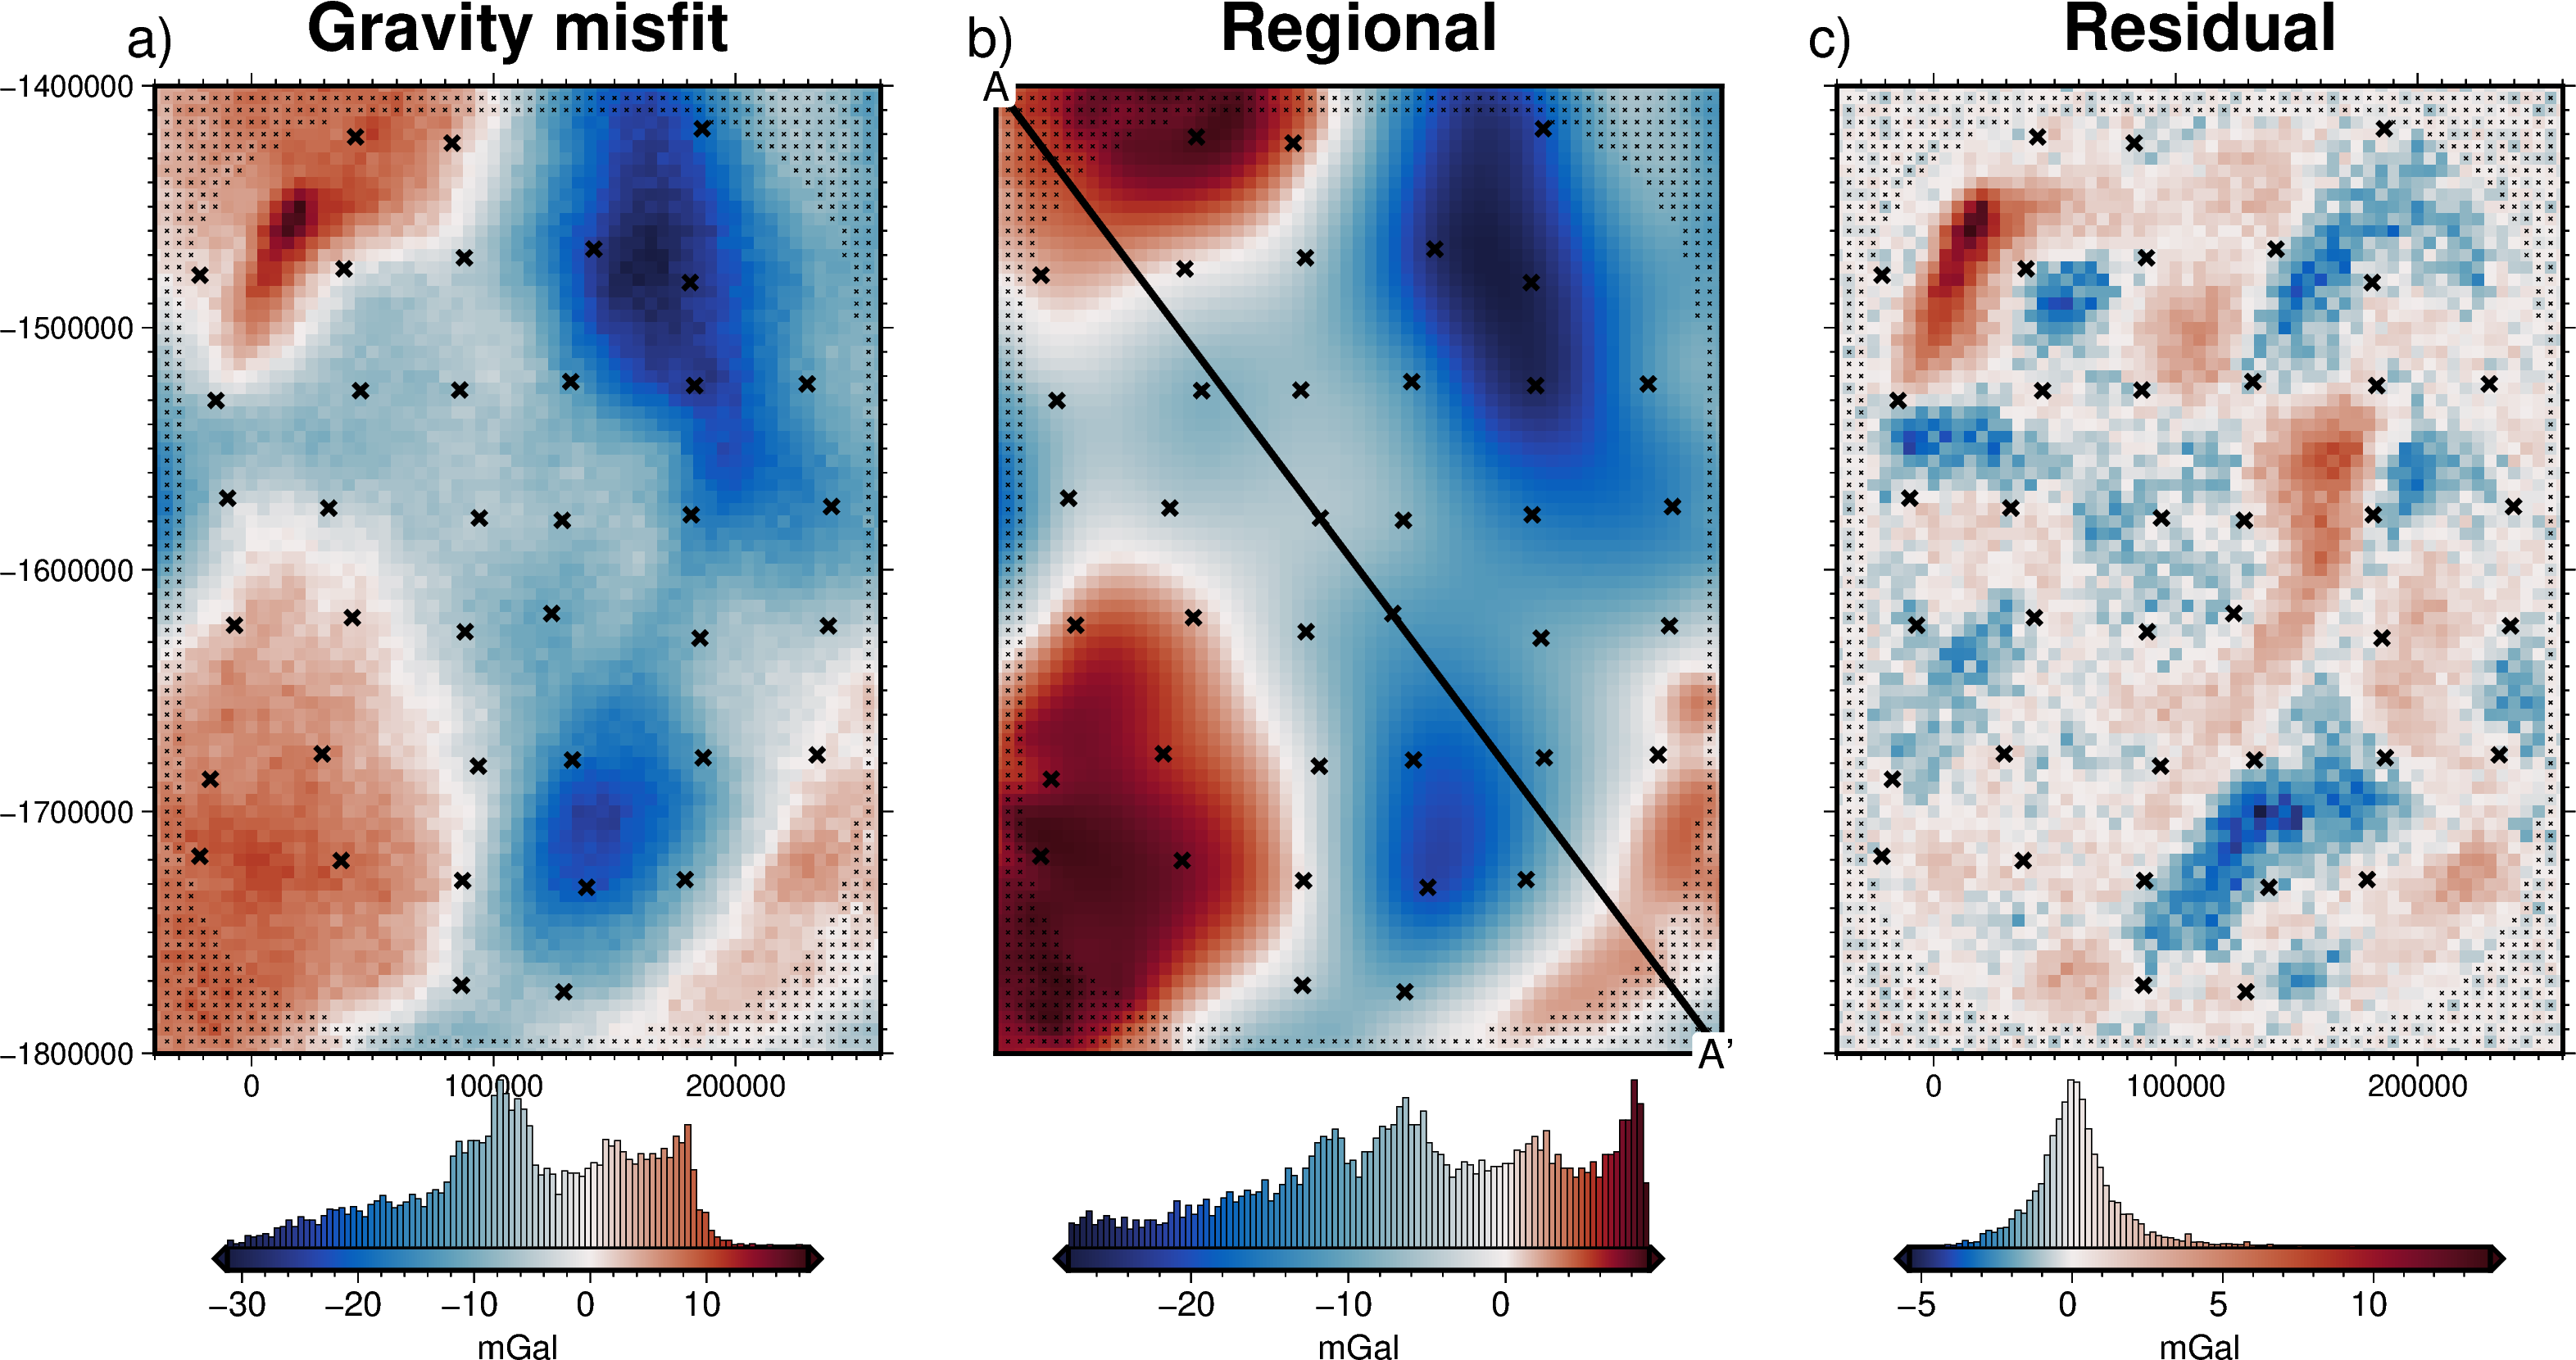
\includegraphics[width=\textwidth]{figures/chp3/chp3_Ross_Sea_misfit.png}
        % \caption{}
    \end{subfigure}
    \begin{subfigure}[t]{.95\textwidth}
        \centering
        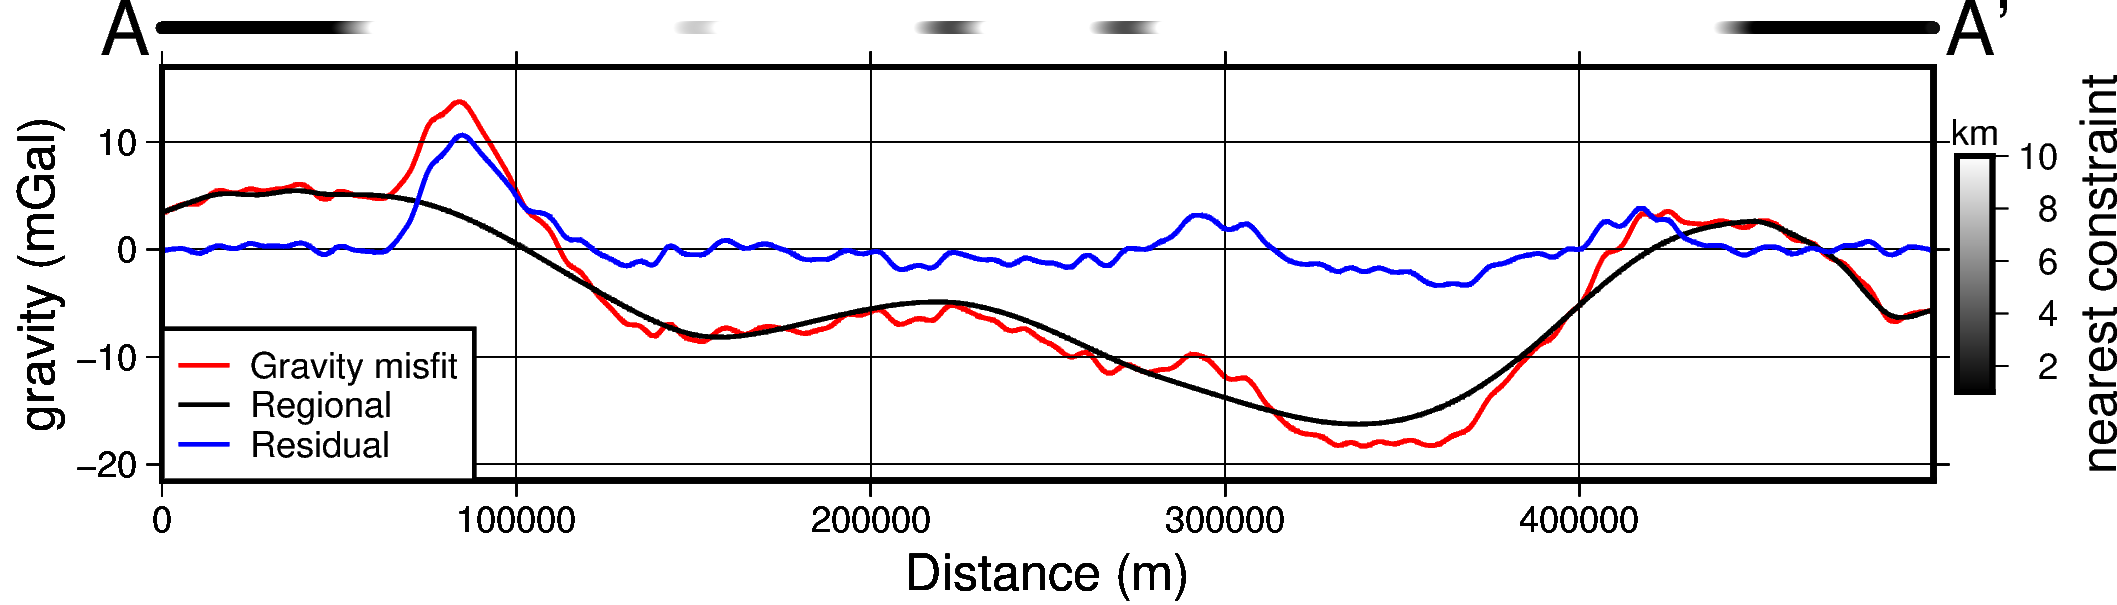
\includegraphics[width=\textwidth]{figures/chp3/chp3_Ross_Sea_misfit_profile.png}
        % \caption{}
    \end{subfigure}
  \caption[Ross Sea synthetic gravity anomalies]{Ross Sea synthetic gravity anomalies. \textbf{a)} total gravity misfit, \textbf{b)} the estimated regional component using the constraint point minimization method, and \textbf{c)}, the residual misfit, as the difference between the total misfit and the regional component. Black crosses, large and small, show constraints inside and outside the ice shelf, respectively. \textbf{Lower panel} shows profile A to A' of gravity misfit and the regional and residual components. Distance to the nearest constraint at each point along the profile shown in black to white colours at top of profile.}
    \label{fig:chp3_Ross_Sea_misfit}
\end{figure}



\subsection{Inversion}

% \begin{wrapfigure}{R}{0.4\textwidth}
%   \centering
%     \includegraphics[width=0.38\textwidth]{figures/chp3/chp3_Ross_Sea_weights.png}
%   \caption{Weighting grid calculated from the minimum distance between each grid cell and the nearest constraint point. These distance are then normalized from 0 to 1.}
%     \label{fig:chp3_Ross_Sea_weights}
% \end{wrapfigure}
% \paragraph{}
% \begin{figure}[!ht]
%     \centering
%     \includegraphics[width=0.4\textwidth]{figures/chp3/chp3_Ross_Sea_weights.png}
%     \caption{Weighting grid calculated from the minimum distance between each grid cell and the nearest constraint point. These distances are then normalized from 0 to 1.}
%     \label{fig:chp3_Ross_Sea_weights}
% \end{figure}

This residual misfit was then used in a cross-validation of 16 damping parameter values (Figure \ref{fig:chp3_Ross_Sea_CV_and_convergence}a). The inversion with the lowest cross-validation score was then chosen as the best model. During the inversions, a weighting grid was used to constrain the bathymetry at the points of known depths (Section \ref{chp3:regularization}). This grid (Figure \ref{fig:chp3_Ross_Sea_starting_model}d) is a normalized (0-1) grid of the minimum distance between each grid cell and the nearest constraint point. The inversion result and the difference from the true bathymetry are shown in Figure \ref{fig:chp3_Ross_Sea_results}. The inversion had an RMS difference with the true Ross Sea bathymetry of 21~m and an RMS at the constraints of $<$~1~m. The inversion converged in 12 seconds at 15 iterations and had a final residual misfit of 0.43~mGal (Figure \ref{fig:chp3_Ross_Sea_CV_and_convergence}b).  \\ 

\begin{figure}[!ht]
  \centering
    \begin{subfigure}[t]{.45\textwidth}
        \centering
        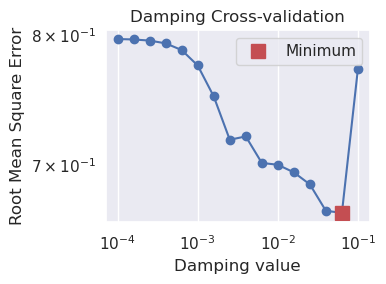
\includegraphics[width=\textwidth]{figures/chp3/chp3_Ross_Sea_CV.png}
        \caption{}
    \end{subfigure}
    \begin{subfigure}[t]{.45\textwidth}
        \centering
        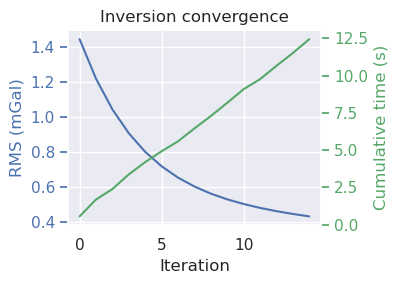
\includegraphics[width=\textwidth]{figures/chp3/chp3_Ross_Sea_convergence.png}
        \caption{}
    \end{subfigure}
  \caption[Ross Sea inversion, CV and convergence]{\textbf{a)} Cross-validation curve showing the optimal damping parameter (red square). \textbf{b)} Convergence of the inversion misfit. Blue line (left y-axis) shows the RMS of the residual misfit at each iteration of the inversion. Green line (right y-axis) shows the cumulative time to complete the inversion. 
  }
    \label{fig:chp3_Ross_Sea_CV_and_convergence}
\end{figure}

\begin{figure}[!ht]
  \centering
    \begin{subfigure}[t]{.9\textwidth}
        \centering
        \includegraphics[width=\textwidth]{figures/chp3/chp3_Ross_Sea_results.png}
        % \caption{}
    \end{subfigure}
    \begin{subfigure}[t]{.7\textwidth}
        % \addtocounter{subfigure}{3}
        \centering
        \includegraphics[width=\textwidth]{figures/chp3/chp3_Ross_Sea_profile.png}
        % \caption{}
    \end{subfigure}
  \caption[Ross Sea inversion results]{Ross Sea synthetic model inversion results. \textbf{a)} True bathymetry, \textbf{b)} difference between a and c, and \textbf{c)} final inverted bathymetry. Black crosses are constraint points. The RMS difference with the true bathymetry at these constraints is $<$~1~m. \textbf{Lower panel)} Profile from A to A'. The top panel contains topographic profiles of the starting, inverted, and true bathymetries. The bottom panel contains gravity anomaly profiles. Distance to the nearest constraint at each point along the profile shown in black to white colours at top of profile.}
    \label{fig:chp3_Ross_Sea_results}
\end{figure}

% \begin{figure}[!ht]
%   \centering
%     \begin{subfigure}[t]{.5\textwidth}
%         \centering
%         \includegraphics[width=\textwidth]{figures/chp3/chp3_Ross_Sea_CV.png}
%         \caption{}
%     \end{subfigure}
%     \begin{subfigure}[t]{.8\textwidth}
%         \centering
%         \includegraphics[width=\textwidth]{figures/chp3/chp3_Ross_Sea_profile.png}
%         \caption{}
%     \end{subfigure}
%   \caption{Cross-validation and profiles for the Ross Sea synthetic inversion with a regional component removed. \textbf{a)} Cross-validation curve showing the optimal damping parameter (red square). \textbf{b)} 2D profile of the inversion results. The top panel shows profile location and constraint points (black crosses). The middle panel contains topographic profiles of the starting, inverted, and true bathymetries. The bottom panel contains gravity anomaly profiles.}
%     \label{fig:chp3_Ross_Sea_CV_and_profile}
% \end{figure}

% \begin{figure}[!ht]
%     \centering
%     \includegraphics[width=0.95\textwidth]{figures/chp3/chp3_Ross_Sea_results.png}
%     \caption{Ross Sea synthetic model inversion results. \textbf{a)} True bathymetry, \textbf{b)} difference between a and c, and \textbf{c)} final inverted bathymetry. Black crosses are constraint points. The RMS difference with the true bathymetry at these constraints is $<$ 1 m.}
%     \label{fig:chp3_Ross_Sea_results}
% \end{figure}

\subsection{Uncertainty analysis} \label{chp3:monte_carlo}

Since the true Ross Sea bathymetry for this inversion is known, a direct measurement of the spatial uncertainty of the resulting bathymetry is simple to calculate (Figure \ref{fig:chp3_Ross_Sea_results}b). This spatial uncertainty is useful to provide alongside the bathymetry results. It informs ocean modellers where results can be confidently interpreted and highlights regions to focus future data collection. Here, a method of uncertainty analysis for this inversion is proposed, and the resulting uncertainty is compared to the inversion error to get a sense of the accuracy of our calculation of uncertainty. This uncertainty analysis is accomplished with Monte Carlo simulations \citep{jansenmonte1994, heltonsurvey2006}. \\

Here, 20 inversions are run with the same damping parameter cross-validation as conducted previously. For each inversion, the input parameters are sampled from distributions of their possible values. These prior distributions represent all plausible parameter values and thus the resulting inverted bathymetries should cover the range of plausible inversion outcomes. For each grid cell, the weighted standard deviation of the 20 inverted bathymetry values of that grid cell was calculated. The weighting came from the inverse square of each inversion's RMS difference between the inverted grid values and the constraint point depths. This reduces the bias from inversions with large misfits to the actual constraint points \citep{schnaidtbootstrap2015}. Chapter \ref{ch:4} Section \ref{chp4_uncertainty_method} contains a detailed description of this uncertainty analysis methodology. \\


% \sigma^*_j = \left[
% \frac
% {\sum_{i=1}^{N}w_i (z_{ij}-\bar{z^*_{ij}})^2}
% {\sum_{i=1}^{N}w_i}  
% \right]^\frac{1}{2},
% \\
% \text{where $z_{ij}$ is the $j^{th}$ cell of the $i^{th}$ inverted bathymetry}

The parameters included in the Monte Carlo sampling are:
\begin{enumerate}
    \item the observed gravity data, sampled from a normal distribution with a mean equal to the observed values and a standard deviation of 0.6~mGal (2\% of the maximum absolute value).
    \item the constraint point depths, sampled from a uniform distribution with a centre as the measured point depth and bounds of $\pm$5~m for the points outside the ice shelf, and $\pm$2\% depth for points within the shelf.
    \item the bathymetry density contrast. This is defined as the difference between the densities of water and sediment. The mean value was taken to be 1276~kg~m\textsuperscript{-1} (2300~-~1024~kg~m\textsuperscript{-1}). A standard deviation of 400~kg~m\textsuperscript{-1} was used.
\end{enumerate} 

\begin{figure}[!ht]
  \centering
    \begin{subfigure}[t]{.9\textwidth}
        \centering
        \includegraphics[width=\textwidth]{figures/chp3/chp3_Ross_Sea_monte_carlo.png}
        % \caption{}
    \end{subfigure}
    \begin{subfigure}[t]{.7\textwidth}
        % \addtocounter{subfigure}{3}
        \centering
        \includegraphics[width=\textwidth]{figures/chp3/chp3_Ross_Sea_monte_carlo_profile.png}
        % \caption{}
    \end{subfigure}
    \caption[Ross Sea Monte Carlo simulation]{Monte Carlo simulation results for the Ross Sea synthetic inversion. Cell-wise weighted standard deviations of all inversions in each simulation. \textbf{a)} Total uncertainty from the sampling of gravity data, constraint depths, and density contrast value. \textbf{b)} Sampling of only the gravity data values. \textbf{c)} Sampling of only the constraint point depths. \textbf{d)} Sampling of only the density contrast. To aid in interpretation, locations outside of the ice shelf have been masked. Constraints within the ice shelf are shown as black crosses in \textbf{d}. \textbf{Lower panel)} Profile from A to A' of the total uncertainty and individual components. Distance to the nearest constraint at each point along the profile shown in black to white colours at top of profile.}
    \label{fig:chp3_Ross_Sea_monte_carlo}
\end{figure}

% \begin{figure}[!ht]
%     \centering
%     \includegraphics[width=0.95\textwidth]{figures/chp3/chp3_Ross_Sea_monte_carlo.png}
%     \caption{Monte Carlo simulation results for the Ross Sea synthetic inversion. Cell-wise weighted standard deviations of all 100 inversions in each simulation. \textbf{a)} Monte Carlo simulation with a pseudo-random sampling of the gravity data values, the constraint point depths, and the prism density values. \textbf{b)} Sampling of only the gravity data values. \textbf{c)} Sampling of only the constraint point depths. \textbf{d)} Sampling of only the density values. All plots share the same color map. To aid in interpretation, locations outside of the ice shelf have been masked. Constraints outside of the ice shelf are shown as small black crosses and constraints within the ice shelf are shown as large black crosses.}
%     \label{fig:chp3_Ross_Sea_monte_carlo}
% \end{figure}

Four suites of Monte Carlo simulations were run and are shown in \ref{fig:chp3_Ross_Sea_monte_carlo}. Each of the above parameters: gravity, constraints, and densities, were included in their own Monte Carlo simulations, and the fourth simulation included all parameters together. Simulations that included the sampling of the constraint depths required the re-calculation of the starting bathymetry, the starting forward gravity, gravity misfit, regional separation, and finally running the inversion. Simulations that included sampling the density values required recalculating the forward gravity, misfit, regional separation, and running the inversion. Simulations that included the sampling of gravity values only required recalculating the regional field and running the inversion. These values were sampled from their respective distributions using Latin hypercube sampling \citep{jansenmonte1994}. This allows an adequate coverage of the parameter space with only 20 inversions. See Chapter \ref{ch:4} Section \ref{chp4_uncertainty_method} for further details.

\subsection{Effects of constraint spacing} \label{chp3:Ross_Sea_constraints_ensemble}

\begin{figure}[!ht]
\captionsetup[subfigure]{labelformat=empty}
  \centering
    \begin{subfigure}[t]{.6\textwidth}
        \centering
        \includegraphics[width=\textwidth]{figures/chp3/chp3_Ross_Sea_constraints_ensemble_graph.png}
        \caption{}
    \end{subfigure}
    \begin{subfigure}[t]{.8\textwidth}
        \centering
        \includegraphics[width=\textwidth]{figures/chp3/chp3_Ross_Sea_constraints_ensemble_errors.png}
        \caption{}
    \end{subfigure}
  \caption[Constraint spacing effects]{Effects of constraint spacing on inversion accuracy. \textbf{a)} Bathymetry error (RMSE) relative to the true bathymetry for 10 different constraint spacing. Green (circles) shows the starting error and blue (diamonds) shows the error after inversion. Labels b, c, and d refer to the three inversion error results shown as subplots. \textbf{b-d)} Inversion error grids for three of the ten configurations of constraints (labelled on a)). Note b-d use the same colour map. Small black crosses show constraints outside the ice shelf, and larger black crosses show inside constraints with the corresponding constraint spacing.}
    \label{fig:chp3_Ross_Sea_constraints_ensemble}
\end{figure}

Here we test the effects of the number and spacing of constraint points on the accuracy of the inversion. The constraints outside the ice shelf are kept as they have been in the previous section, at the same grid spacing as the bathymetry (5~km). Constraints within the ice shelf are re-created on a regular grid, where the spacing of the grid, and thus the number of constraints, is varied from 10~km (959 constraints) to 100~km (9 constraints). The depth of the true bathymetry is sampled at each constraint. As in the previous section, points outside the shelf are contaminated with Gaussian noise with a standard deviation of 5 m. Noise for constraints within the ice shelf is relative to each point's depth (to simulate seismic survey uncertainties). These  noise-contaminated constraint point depths are used in a bi-harmonic spline gridding to create the starting bed for each of the 10 constraint sets. The RMS difference between each of the starting beds and the true bed is shown as green dots in Figure \ref{fig:chp3_Ross_Sea_constraints_ensemble}a. From these starting beds the inversion workflow was conducted, as below:

\begin{enumerate}
    \item The forward gravity of the starting beds were calculated.
    \item The misfits with the observed gravity (Figure \ref{fig:chp3_Ross_Sea_survey}a) were calculated\footnote{To isolate the effects of changing the constraint density, the full resolution observed gravity with no added noise was used here, instead of the synthetic survey gravity.}.
    \item The regional component of the misfit was estimated and removed with the constraint point minimization method.
    \item The residual misfit was inverted with the cross-validation routine.
    \item The difference between each inverted bed and the true bed was found.
\end{enumerate}

Figure \ref{fig:chp3_Ross_Sea_constraints_ensemble} shows the results of this analysis. Subplot a) shows the relationship between constraints spacing and the RMSE with the true bed of the starting bed (green circles) and the final inverted bed (blue diamonds). Three of the inverted bed errors are shown in subplots b-d. See Appendix \ref{appB_Ross_Sea} for plots of the regional separation errors for these three inversions. 


\subsection{Effects of gravity data} \label{chp3:Ross_Sea_gravity_ensemble}

As the above section analyzed the impact of the number of constraint points on the inversion's accuracy, here we investigate the impact of the quality and quantity of input gravity data. Following the methods of the two ensembles presented in the simple synthetic inversion (Figure \ref{chp3:simple_ensemble} \& \ref{fig:chp3_simple_regional_ensemble}), an ensemble of 100 inversions with varying levels of noise and gravity observation spacing's are conducted with this Ross Sea model. The observed gravity data were contaminated with noise as described in the past sections, with 10 levels between 0 and 9\% of the maximum absolute value. To simulate a more spare gravity survey, the previous two ensembles sampled the full-resolution gravity data onto a coarser evenly spaced grid and then re-gridded the sparse data with equivalent sources back to the full resolution of the bathymetry. Here instead of evenly spaced grids, we use airborne flight lines. \\

We use a constant along-line observation spacing of 5~km but vary the spacing between flight lines. The N-S and E-W lines both use the same between-line spacing. The full-resolution gravity is then sampled at these points, and the sparse data is re-gridded to the full resolution (5~km) with equivalent sources. The noise and line spacing changes were applied to the original observed data, and the forward calculation of the starting model, initial misfit calculation, and regional field removal were all repeated. Each model was then inverted with a cross-validation, and the resulting RMS differences with the true bathymetry are shown in Figure \ref{fig:chp3_Ross_Sea_gravity_ensemble}. 

\begin{figure}[!ht]
    \centering
    \includegraphics[width=0.9\textwidth]{figures/chp3/chp3_Ross_Sea_gravity_ensemble.png}
    \caption[Ross Sea ensemble of noise levels and gravity spacing]{Ensemble of noise levels and airborne gravity line spacing for the Ross Sea synthetic model. Grid cell colour indicates each inversion's RMSE with the true bathymetry. Circles' colour indicates the optimal damping value found for each inversion's cross-validation. Black line shows the 34~m contour which represents the RMS difference between the true and starting bathymetry (Figure \ref{fig:chp3_Ross_Sea_starting_model}b).}
    \label{fig:chp3_Ross_Sea_gravity_ensemble}
\end{figure}


\section{Discussion}

\subsection{Simple synthetic model}

The simple synthetic model of Section \ref{chp3:simple_model} was introduced to 1) present the basic workflow of the inversion, 2) determine the best options for various components of the inversion and 3) demonstrate the capabilities and limitations of the inversion. The starting bathymetry had an RMS difference with the true bathymetry of 66~m (Figure \ref{fig:chp3_simple_starting_model}). This error demonstrates the limitations of gridding sparse data. Even with a very high spatial constraint density (1 constraint per 160~km\textsuperscript{2}) compared to most ice shelves \citep{fretwellbedmap22013}, simply gridding the constraints greatly misinterpreted the true bathymetry. To reduce this bathymetric error, we presented three inversions, a noise-free full-resolution inversion, a noise-contaminated full-resolution inversion, and a noise-free lower-resolution inversion.

\subsubsection{Inversion results}

All of these inversions (without a regional component) were able to reduce this RMS difference with the true bathymetry to $\sim$~10~m and recover all bathymetric features of interest. We demonstrated that the two methods of calculating the vertical derivative of gravity produced similar results, but the annulus approximation was significantly faster ($\sim$5$\times$). Additionally, for each of these inversions, the weighting grid, based on the distance to the nearest constraints (Figure \ref{fig:chp3_simple_weights}), successfully constrained the resulting inverted bathymetry at the points of prior bathymetry observations. Each inversion's constraint point RMS difference with the true bathymetry was $<\sim$2~m, and the technique avoided any pedestal effect around the constraints in the resulting bathymetries. Interestingly, the inversion with low-resolution (6~km) gravity data yielded a very similar RMSE compared to the inversion with the full-resolution (1~km) data. This demonstrates that for recovering bathymetric features of wavelengths similar to those found in our synthetic model, high-resolution gravity surveys may not be necessary to achieve adequate results from an inversion. 

\subsubsection{Ensemble results}

To test this theory further, we conducted an ensemble of 100 inversions with 10 levels of noise contamination and 10 gravity survey resolutions. The resulting RMS difference of each inversion with the true bathymetry is shown in Figure \ref{fig:chp3_simple_ensemble}. All inversions in this ensemble, including the worst-case scenario of 9\% noise and a gravity observation grid of 10$\times$ the bathymetry spacing, still resulted in an RMS difference lower than that of the starting bathymetry (66~m). It is worth noting that this metric for the accuracy of the inversion, the root mean squared (RMS) difference with the true bathymetry, is used to give extra weighting to the outlier errors, as opposed to using a mean average error (MAE). These outliers typically include the features of interest in a bathymetry inversion. Figure \ref{fig:chp3_simple_ensemble_lines}a shows these ensemble results grouped by cell size. For each cell size value (colour of lines), the inverted bed RMSE for the range of noise levels is shown. This shows a roughly linear relationship between noise and RMSE, regardless of cell size. This means there is a continuous improvement in the inversion's accuracy with lower levels of noise. Conversely, figure \ref{fig:chp3_simple_ensemble_lines}b shows these ensemble results grouped by the noise level. For each noise level (colour of lines), the inverted bed RMSE for the range of cell sizes is shown. This shows an exponential relationship between gravity survey resolution and RMSE. This exponential relationship is strongest for low noise levels. This means inversion accuracy greatly benefits from increasing the survey resolution (decreasing the cell size), but this benefit diminishes once the survey resolution is at a certain point. Here, surveys at or below $\sim$6~km resolutions result in a diminishing improvement in RMSE. The linear relationship between noise and RMSE, and the exponential relationship between resolution and RMSE can also be seen by the spacing of lines in either figure. The close spacing of the low-cell-size lines (purples) in Figure \ref{fig:chp3_simple_ensemble_lines}a show the diminishing improvements at small cell size surveys, while the continuous spacing of lines in Figure \ref{fig:chp3_simple_ensemble_lines}b shows the linear relationship. \\

\begin{figure}[!ht]
  \centering
    \begin{subfigure}[t]{.48\textwidth}
        \centering
        \includegraphics[width=\textwidth]{figures/chp3/chp3_simple_ensemble_noise_lines.png}
        \caption{}
    \end{subfigure}
    \begin{subfigure}[t]{.48\textwidth}
        \centering
        \includegraphics[width=\textwidth]{figures/chp3/chp3_simple_ensemble_cellsize_lines.png}
        \caption{}
    \end{subfigure}
  \caption[Grouped synthetic inversion ensemble]{Ensemble results for the simple synthetic inversion, grouped by \textbf{a)} gravity survey cell size, and by \textbf{b)} noise level. Each line in a) corresponds to a row of Figure \ref{fig:chp3_simple_ensemble} and each line in b) corresponds to a column.}
    \label{fig:chp3_simple_ensemble_lines}
\end{figure}

In a typical gravity survey, there is often a trade-off between the number of observations made and the quality (noise) of the data. This is due to the time restrictions of both the total data collection period (i.e. the length of a field season in Antarctica), and the necessity to repeat base-station measurements to account for instrument drift. Collecting more data in the same time period inevitably results in increased noise. At a certain point, this increased noise will have a greater negative effect on the inversion results, than will be counteracted by the increased amount of data. These are important considerations for survey design. Figure \ref{fig:chp3_simple_ensemble_lines}b shows that for a given noise level, there is little benefit in increasing the gravity survey resolution from $\sim$6~km to 1~km. For this survey domain (60~$\times$~80~km), a 6~km resolution results in $\sim$130 gravity station, while with a 1~km resolution, this increases to 4800 observation points. Simplistically speaking, if keeping total survey time constant, this means at 6~km spacing as opposed to 1~km spacing, either $\sim$36$\times$ more area could be surveyed, or higher quality data could be collected, with shorter base station loops, more repeated ties, and more careful measurements. \\

The results from the noise-contaminated inversion (Figure \ref{fig:chp3_simple_noise_results} \& \ref{fig:chp3_simple_CV_and_profile}b) show that this gravity noise is directly reflected in the inversion results. For this reason, data, either the observed data or the residual misfit, is typically low-pass filtered prior to inversion \citep[i.e.][]{boghosianresolving2015, yangocean2020}. This is typically done with either a time-based filter for airborne surveys, or a spatial filter \citep{jordanaerogravity2010}. With this filtering, there is a trade-off between removing the noise and removing the true signal. Due to this, we have chosen to omit the filtering in these synthetic examples.

\subsection[Regional component]{Simple model with a regional component\sectionmark{Regional component}}

\subsubsection{Regional separation methods}

The addition of a regional component to the observed gravity data adds a major complexity to the inversion workflow. The actual inversion remains the same, but this regional component must be estimated and removed beforehand. We tested four methods of regional estimation; 1) a low-pass filter, 2) fitting a polynomial trend to the data, 3) predicting the data with a set of deep point sources, and 4) attributing the entire misfit value to the regional field at constraint points and interpolating between these values. Figure \ref{fig:chp3_simple_regional_comparison} compares the inversion results of each of these methods. While each method recovered the short wavelengths bathymetry features, the misestimation of the true regional field for each method introduced long-wavelength errors in the inversion results. We show that the constrain point minimization method most accurately estimated the region, and thus produced the best inversion results. For the simple regional field used here, the filter and trend methods achieved reasonable results, but the effectiveness of these methods is expected to be reduced with more complex regional fields associated with real data. \\

While the constraint point minimization worked best for this model, each of these methods may work better in specific scenarios. All the methods except the equivalent source method require the gravity data to be gridded over the entire region of interest. For sparse gravity surveys the interpolation required may introduce large errors. For this scenario, the equivalent source technique is likely the most appropriate. In scenarios with few bathymetry constraints and where the regional field is expected to be simple, the trend and low-pass filter methods are efficient and can be effective. However, if there are distributed bathymetry constraints, such as in this synthetic scenario, constraint point minimization is likely the best choice. This technique will only effectively remove regional anomalies with a wavelength equal to or greater than the average constraint spacing. If the constraints are sparse relative to the expected regional anomaly wavelengths, this method will underestimate the regional component. Lastly, if the bathymetry contains long-wavelength features which would result in long-wavelength anomalies, the trend, filter, and equivalent source techniques may include these in the regional removal. Therefore, the inverted bathymetry, while recovering the super-imposed short-wavelength bathymetry features, will underestimate the long-wavelength features. It is for these reasons that regional separation is perhaps the most important aspect of a bathymetry inversion. 

\subsubsection{Constraint point minimization}

This constraint point minimization technique requires the gridding of sparse measurements of the regional field. We explored the impact of this gridding process on the resulting inversion. Figure \ref{fig:chp3_simple_regional_gridding_comparison} shows the results of four different gridding processes. Minimum curvature gridding without tension (tension of 0, Figure \ref{fig:chp3_simple_regional_gridding_comparison}a) produces a smoothly varying surface at the constraints but introduces artificial minima and maximum at points far from any constraints. This erroneous effect is minimized with a higher tension factor. Using a tension factor of 1, figure \ref{fig:chp3_simple_regional_gridding_comparison}c shows the limited erroneous minima and maxima, but this added tension results in high gradients in the surface immediately near the constraint points (Figure \ref{fig:chp3_simple_regional_gridding_comparison}g). These high gradients in the resulting residual anomalies create a \textit{ringing} effect in the inverted bathymetry (Figure \ref{fig:chp3_simple_regional_gridding_comparison}k). For these reasons, an intermediate tension factor of 0.25 is suggested for potential field data. While this limits the negative effects of both low and high tension, there are still false minima and maxima (Figure \ref{fig:chp3_simple_regional_gridding_comparison}b), and high gradients at the constraints (Figure \ref{fig:chp3_simple_regional_gridding_comparison}f). The last gridding technique uses bi-harmonic splines. The optimal damping parameter associated with this technique is chosen from a cross-validation of the constraint points. This technique, while being more computationally expensive, solves both issues of tensioned minimum curvature. 

\subsubsection{Inversion results}

\begin{figure}[!ht]
    \centering
    \includegraphics[width=.7\textwidth]{figures/chp3/chp3_simple_regional_bed_error.png}
    \caption[Synthetic inversion error and regional error]{Source of inverted bathymetry error for the simple synthetic model with a regional field. \textbf{a)} Inverted bathymetry error from Figure \ref{fig:chp3_simple_regional_results}b. \textbf{b)} Error in the estimation of the regional component of gravity from comparison with the true regional component (Figure \ref{fig:chp3_simple_regional_gravity}b). Black crosses show constraint points. Colourmaps are inverted to highlight the similarities and the median has been removed from the regional error.}
    \label{fig:chp3_simple_regional_bed_error}
\end{figure}

With both the optimal regional separation method and the optimal gridding method determined, we performed a cross-validated inversion with the remaining residual misfit. This inversion was able to recover all the short-wavelength bathymetry features but introduced some long-wavelength errors. Figure \ref{fig:chp3_simple_regional_bed_error} shows the inverted bathymetry error alongside the error in estimating the regional component of gravity. Comparing these shows that almost all of the inverted bathymetry error is tied to the inaccuracies of determining the regional component. the remaining error is all minor short-wavelength features, mostly around constraint points. They appear to result from the weighting grid implementation of regularization. Since the errors in the regional estimation are the dominant source of error in most inversions, as shown above, and by other Antarctic bathymetry inversions \citep{brisbourneseabed2014}, we have shown these details of the gridding process are a vital and often overlooked step in many studies. 

\subsubsection{Ensemble results}

As with the simple model, an ensemble of noise and gravity survey spacing experiments were performed with this model containing a regional component. The lowest resulting RMS difference with the true bathymetry was raised from values of $\sim$10~m for the inversion without the regional component, to the lowest value of $\sim$~40 m with the additional regional component. The black line in Figure \ref{fig:chp3_simple_regional_ensemble} shows the 66~m contour, which represents the RMS difference between the true and starting bathymetries. Inversions that fall outside (above) this line resulted in a worse bathymetry than the starting model. This shows that for this model, inversion is only worth conducting if the gravity survey has a spacing less than $\sim$9~km ($\sim$9$\times$ the spacing of the desired bathymetry resolution). Figure \ref{fig:chp3_simple_regional_ensemble_lines} show these ensemble results grouped by cell size and noise level. There is a linear relationship between gravity noise and the resulting bathymetry RMSE, for all gravity survey spacings. There is an approximately exponential relationship between gravity survey resolution (cell size) and resulting bathymetry RMSE. The degree of this exponential relation decreases with increased noise. \\

For this model, the \textit{elbow} of the exponential curves in Figure \ref{fig:chp3_simple_regional_ensemble_lines}b is at $\sim$ 6~-~8~km survey resolutions (6-8$\times$ bathymetry resolution). This suggests that for a survey resolution finer than $\sim$8~km, there is little benefit in collecting more data. This is supported by the close spacing of low-cell-size lines (purples) in Figure \ref{fig:chp3_simple_regional_ensemble_lines}a. The effort would be better spent collecting data over a wider region, reducing noise in the data, or if possible collecting more bathymetric constraints.

\begin{figure}[!ht]
  \centering
    \begin{subfigure}[t]{.48\textwidth}
        \centering
        \includegraphics[width=\textwidth]{figures/chp3/chp3_simple_regional_ensemble_noise_lines.png}
        \caption{}
    \end{subfigure}
    \begin{subfigure}[t]{.48\textwidth}
        \centering
        \includegraphics[width=\textwidth]{figures/chp3/chp3_simple_regional_ensemble_cellsize_lines.png}
        \caption{}
    \end{subfigure}
  \caption[Grouped synthetic inversion with regional ensemble]{Ensemble results for the synthetic inversion with a regional component, grouped by \textbf{a)} gravity survey cell size, and by \textbf{b)} noise level. Each line in a) corresponds to a row of Figure \ref{fig:chp3_simple_regional_ensemble} and each line in b) corresponds to a column.}
    \label{fig:chp3_simple_regional_ensemble_lines}
\end{figure}

\subsection{Ross Sea model}

The Ross Sea semi-realistic model was created to better emulate the gravity and bathymetries expected for ice shelves. A few extra complexities were added to this model compared to the purely synthetic models. An ice shelf border was included, with a high density of constraints outside of the border, and sparse constraints within. All the constraints had an associated uncertainty, instead of directly sampling the true bathymetry depths. The observed gravity was calculated along the flight paths of a typical airborne survey, instead of along a uniform grid. The main inversion in this section had 2\% noise added and had flight lines with 50~km N-S spacing and 15~km E-W spacing. The inversion successfully reduced the starting bathymetry error from an RMSE of 34~m to 23~m. The resulting bathymetry shows a recovery of most of the lost bathymetry features, but some noise from the gravity data has been introduced into the bathymetry. Sharp bathymetry features (upper left corner) and smooth features were both recovered. The constraint points were relatively evenly distributed (Figure \ref{fig:chp3_Ross_Sea_starting_model}d), resulting in a relatively even distribution of bathymetry misfits. \\

Of these errors, the largest were located at the gaps in the synthetic survey where there were missing flight lines (Figure \ref{fig:chp3_Ross_Sea_survey}b). To understand the cause of the remaining errors, we compare the inverted bathymetry error with the regional separation error (Figure \ref{fig:chp3_Ross_Sea_regional_bed_error}). The strong correlation between these two grids shows that the majority of errors in the inversion are tied to the miscalculation of the regional field, as was seen in the simple synthetic inversion with a regional field. The remaining errors appear to be from the flight line gaps and noise in the gravity data. 

\begin{figure}[!ht]
    \centering
    \includegraphics[width=.7\textwidth]{figures/chp3/chp3_Ross_Sea_regional_bed_error.png}
    \caption[Ross Sea inversion error and regional error]{Comparison of the inverted bathymetry error and the error in the regional field estimation. \textbf{a)} Inverted bathymetry error from Figure \ref{fig:chp3_Ross_Sea_results}b. \textbf{b)} Error in the estimation of the regional component of gravity from comparison with the true regional component (Figure \ref{fig:chp3_Ross_Sea_layers_and_forwards}d). Black crosses show constraint points. Colourmaps are opposed to highlight the similarities and the median has been removed from the regional error.}
    \label{fig:chp3_Ross_Sea_regional_bed_error}
\end{figure}

\subsubsection{Effects of the gravity data} \label{chp3_effect_of_gravity_noise}

The ensemble of gravity data noise levels and flight line spacings from Section \ref{chp3:Ross_Sea_gravity_ensemble} shows the relative importance of these two aspects of a gravity survey. As for the previous ensembles, Figure \ref{fig:chp3_Ross_Sea_gravity_ensemble_lines} shows these results grouped by line spacing and by the noise level. For the Ross Sea model, both factors have a roughly linear relationship with inverted bathymetry error. The slopes for the lines of best fit for Figure \ref{fig:chp3_Ross_Sea_gravity_ensemble_lines}a and b means the inversion RMSE increases by $\sim$10~m for either a 4\% increase in the noise level or a 60~km increase in the average flight line spacing. The inversions with a small line-spacing (purple lines) of Figure \ref{chp3:Ross_Sea_gravity_ensemble}a are closely grouped, relative to the higher line spacings. This shows that at already low line spacings (40~km) there may be little benefit to reducing the line spacing further. Conversely, there is a larger spread for the low noise inversions (purple lines) in Figure \ref{chp3:Ross_Sea_gravity_ensemble}b. This shows that even at low noise levels, further decreases may still provide important improvements to the inversion outcome. As in the previous ensemble results, for a field application, this demonstrates the important tradeoff between quantity and quality of gravity data. \\

\begin{figure}[!ht]
  \centering
    \begin{subfigure}[t]{.48\textwidth}
        \centering
        \includegraphics[width=\textwidth]{figures/chp3/chp3_Ross_Sea_gravity_ensemble_noise_lines.png}
        \caption{}
    \end{subfigure}
    \begin{subfigure}[t]{.48\textwidth}
        \centering
        \includegraphics[width=\textwidth]{figures/chp3/chp3_Ross_Sea_gravity_ensemble_spacing_lines.png}
        \caption{}
    \end{subfigure}
  \caption[Grouped Ross Sea inversion with regional ensemble]{Ensemble results for the Ross Sea inversion, grouped by \textbf{a)} gravity survey line spacing, and by \textbf{b)} noise level. Each line in a corresponds to a row of Figure \ref{fig:chp3_Ross_Sea_gravity_ensemble} and each line in b corresponds to a column. Red lines show the line of best fit, with their slopes shown in the upper left corners.}
    \label{fig:chp3_Ross_Sea_gravity_ensemble_lines}
\end{figure}

These specific relationships between noise, line spacing, and inversion error, while not applicable to all survey configurations, show the importance of choosing an appropriate survey design. This analysis with synthetic data could be included in a pre-survey plan, to explore the effects of differing survey configurations. 

\subsubsection{Effects of the constraints} \label{chp3_effect_of_constraints}

These synthetic inversions have shown that the removal of the regional field presents the biggest challenge for gravity inversions for bathymetry. The most robust technique for removing the regional field requires a distribution of points of known bathymetry across the inversion region. Since the largest errors in the inverted bathymetries occur at the largest distance to constraints, an even distribution of constraints will best be able to estimate the regional field. Section \ref{chp3:Ross_Sea_constraints_ensemble} explored the effects of varying the numbers of constraints, while keeping the remaining components of the inversion constant. Figure \ref{fig:chp3_Ross_Sea_constraints_ensemble}a shows the bathymetry RMSE with the true bathymetry both before (green) and after (blue) the inversion is conducted. \\

Figure \ref{fig:chp3_Ross_Sea_constraints_ensemble}a shows for this synthetic model that for average constraint spacing's less than $\sim$20~km there is little improvement made by running an inversion. This is due to the starting bathymetry model already being relatively accurate, with the inversion only producing minor adjustments between constraint points. At the other end of the spectrum, with constraint densities greater than $\sim$70~km, the inverted bathymetry has an error similar to or higher to the un-inverted bathymetry. This is due to the inaccuracies in calculating the regional field with only very sparse constraints. For these scenarios, the errors introduced by the inversion are greater than the errors of simply interpolating the constraint points. The inverted bathymetry error curve (Figure \ref{fig:chp3_Ross_Sea_constraints_ensemble}a) shows that for this survey, once below a certain constraint spacing ($\sim$30~km) there is little benefit to having additional constraints. 

\subsubsection{Uncertainties}
We have demonstrated that the majority of the inverted bathymetry error is related to the estimation of the regional component of gravity. Without knowing the true regional component, as we do in these synthetic examples, estimating the uncertainty in the interpolation between constraint points of the regional field is difficult. The uncertainty of each grid cell is likely strongly dependant on the distance to the nearest constraint, as well as the depth uncertainties of these nearby constraints. While we show this to be true with our synthetic models, a quantitative method of predicting this uncertainty has yet to be implemented here. The field of conventional bathymetry surveying has developed uncertainty analysis tools that may be applicable to this \citep{bourgeoisachieving2016}. \\

These tools are able to account for both the depth uncertainty of each measurement, and the distance of each grid cell to the nearest measurement. Future work will benefit from a quantitative assessment of the uncertainty of gridding the regional field from the constraint point values. While the uncertainty of the regional removal accounts for the majority of the uncertainty of the inverted bathymetry, it is technically completed before the inversion and is thus not a component of the inversion uncertainty. To address the uncertainty resulting from the inversion process, we introduced a suite of Monte-Carlo simulations in Section \ref{chp3:monte_carlo}. The results in figure \ref{fig:chp3_Ross_Sea_monte_carlo} show a mean uncertainty for the entire region of 22 m. The majority of this uncertainty is attributed to the uncertainty in the gravity data, as shown by histograms of Figure\ref{fig:chp3_Ross_Sea_monte_carlo}. Here we discuss the significance of each component of the uncertainty analysis:

\begin{enumerate}
    \item \textbf{Gravity uncertainty:} The uncertainties in the gravity data result in a relatively uniform bathymetry uncertainty across the region of 17~m. A simple calculation with the Bouguer slab formula with a density contrast of 1276~kg~m\textsuperscript{-3} and our assumed gravity uncertainty of 0.612~mGal (\%2 max absolute value) gives a value of 11.5~m ($\Delta g_{boug}= 4.18\text{e-}5 \rho h$). This may show the conventionally used Bouguer slab approximation is underestimating the true uncertainty in inversions resulting from gravity data uncertainty. This uncertainty is lowest at the constraints, due to the use of the weighting grid in the inversion. 

    \item \textbf{Constraint depth uncertainty:} The contribution to the bathymetry uncertainty from the depth uncertainty of the constraint points is small, with a mean of $\sim$4~m. This uncertainty resulting from the constraints is also concentrated around the constraint points. This shows improving the constraint point uncertainties will not greatly improve the inversion, and will only improve it in the immediate vicinity of constraints. 

    \item \textbf{Density uncertainty:} The bathymetry uncertainty component resulting from the prism densities is heterogeneous, with some spatially limited, but large values. The mean value is $\sim$11~m, but some areas are up to 50~m. These high uncertainties are strongly correlated with the error in the starting bathymetry (Figure \ref{fig:chp3_Ross_Sea_starting_model}b). This is due to the change in density contrast resulting in a change in the total bathymetry correction calculated in the inversion. In other words, the residual misfit can be minimized by a large surface correction with a low-density contrast or a small surface correction with a large-density contrast. 
\end{enumerate}

The combined Monte-Carlo simulation (Figure \ref{fig:chp3_Ross_Sea_monte_carlo}a) shows the expected features of an uncertainty map. It has a base level uncertainty similar to the Bouguer slab thickness from the assumed gravity uncertainty, it is generally lowest at the constraints and highest in the large constraint gaps, and it is high where the inversion has produced a large change from the starting model.

\section{Future work}

Running this inversion with the various synthetic models gave us the ability to assess the inversion performance. From this assessment, we have determined several components which would benefit from additional investigation. 

\begin{enumerate}
    % \item Test the effects of the relative strengths of the regional and residual components.
    \item Implement an additional cross-validation routine to estimate the optimal density contrast, as in \citet{uiedafast2017}. Here, we have used the same density contrasts for the creation of the observed gravity data and for the inversion itself. In a non-synthetic scenario, this contrast would need to be estimated.
    \item Test the effects of flight line orientation relative to the dominant trend of geologic structures.
    \item Implement a more robust method of enforcing the constraint points. This may likely be in the form of a bounded least squares solver or some form of manipulation of the Jacobian matrix. 
    \item Quantify the uncertainty of the regional separation process. This will likely include techniques used in conventional bathymetry surveying \citep{calderdevelopment2017, bourgeoisachieving2016}, or a sequential Gaussian simulation \citep{perozziquantitative2021}.
    % \item Include the equivalent source gridding of the observed gravity data in the Monte Carlo analysis to see the effects of the entire workflow, not just the inversion.
    % \item Perform a three-way comparison of the effects of constraint spatial density, gravity survey spacing, and gravity noise.
    \item Testing the effects of pre-filtering the gravity data, either spatially or temporally, to remove the effects of noise \citep{jordanaerogravity2010}.
\end{enumerate}

\section{Conclusion}

With the goal of modelling the bathymetry beneath a floating ice shelf, we present a geometric gravity inversion method that 1) adheres to prior bathymetry point measurements, within their uncertainties, 2) produces a smooth and realistic bathymetry, 3) accounts for the regional gravity field and 4) is computationally efficient and fully-open source. To demonstrate the effectiveness, as well as the limitations, we conducted a series of inversions using synthetic and semi-realistic data. These inversions showed the importance of accurately estimating and removing the regional component of gravity prior to the inversion. We showed that for the constraint arrangement for many Antarctic ice shelves, the optimal method for estimating this regional field is with a constraint-point minimization. In addition, we further explored this method by testing various gridding (interpolation) techniques and found a clear increase in performance when using a cross-validated bi-harmonic spline instead of the typically used tensioned minimum curvature. \\

Here we reiterate a few of the key findings from this chapter:
\begin{enumerate}
    \item 
    Estimating and removing the regional component of gravity for typical inversion scenarios is the most important aspect of the inversion procedure. For typical bathymetry inversions, the optimal method for estimating the regional field is constraint point minimization.
    \item 
    When collecting data for an inversion, it is best to aim for quality over quantities for the gravity data, and conversely, quantity over quality for bathymetry constraint measurements.
    \item 
    We provide general guidelines on the optimal ranges of constraint density, gravity survey line spacing, and gravity noise, for which conducting an inversion is suitable. 
\end{enumerate}

Testing the various models with differing levels of gravity noise and numbers of gravity observation points highlights an important factor in planning a gravity survey. We show for the Ross Sea synthetic model, which likely emulates the scenario expected from many Antarctic ice shelves, \textbf{there are diminishing returns for average flight line spacings smaller than $\sim$40~km} if the goal is to recover bathymetry features typical of the Ross Sea. \textbf{However, the inverted bathymetry's accuracy is strongly affected by noise in the gravity data.} With this, the typically airborne survey focus on quantity over quality may need to be reassessed. If 40~km spaced flight lines produce similar results to 20~km lines, flying half the number of lines will save a significant amount of time. This time could be used to either expand the area of the survey or reduce the noise in the data. Reducing the data noise for an airborne survey may not always be feasible, but a few measures may be taken to attempt this, all of which are aided by the increased survey time allowed by reducing the number of flight lines. These include repeating lines or sections which are noisy, limiting flights to good weather windows, increasing the number of tie-lines, making shorter loops for base-station ties, or flying at lower altitudes and or ground speeds.  \\

\textbf{The previous measurements of bathymetry, referred to as the constraints, are a vital part of an inversion for bathymetry.} Due to the non-uniqueness of an inversion, there are an infinite number of inverted bathymetry models which will equally match the observed data. These constraints provide the ground truth necessary to confidently chose a model out of these infinite choices. Additionally, if not more importantly, they provide the primary method of accounting for the regional component of gravity. Since this is shown to be the largest source of uncertainty, the constraints are the most important aspect of the inversion. We tested the effects of varying the spatial density of the constraint points. The results (Figure \ref{fig:chp3_Ross_Sea_constraints_ensemble}) show the range of constraint point spacings for the Ross Sea synthetic model which justifies conducting a gravity inversion if the goal is to recover bathymetry with a 5~km resolution. \\

\textbf{The optimal constraint spacing is $\sim$20-70~km.} Smaller spacing values already have an adequate amount of information and little is gained over a simple interpolation of the data. At spacings larger than $\sim$70~km, the errors in estimating the regional field are larger than the improvements made by the inversion. These values, while specific to the Ross Sea scenario, provide an important context for the feasibility of conducting bathymetry inversions. Taken together with the above assessment of the relative importance of gravity data noise and density, some general guidelines are provided. \\

As long as the gravity data is on the order of magnitude of 2-4$\times$ the spacing of the desired bathymetry resolution, and the noise levels are low, \textbf{efforts should be focused on collecting more bathymetry measurements.} The uncertainty of these depth measurements is relatively unimportant (Figure \ref{fig:chp3_Ross_Sea_monte_carlo}c), meaning quantity over quality is acceptable here. The final spatial uncertainty of the inverted bathymetry is strongly tied to the distance to the nearest constraint. This suggests that an even distribution of the constraints is important. However, if specific regions of the survey are expected to have larger amplitude regional anomalies, an increased spatial density of constraints over this region would be beneficial. With these recommendations, future planning for Antarctic fieldwork should be able to collect data that prioritizes the accurate assessment of sub-ice-shelf bathymetry.  \\

Chapter \ref{ch:4} applies the inversion presented here to model the bathymetry beneath Antarctica's Ross Ice Shelf. 


\chapter{Ross Ice Shelf bathymetry inversion}
\label{ch:4}
\chaptermark{bathymetry}
% Mapping spatiotemporal patterns of Antarctic subglacial lake drainage and filling events

\section*{Abstract}

To examine an aspect of subglacial water movement in Antarctica, we present a new map of active subglacial lakes inferred from spatiotemporal patterns of ice surface elevation trends.
An unsupervised density-based classification technique is applied to pre-processed ICESat-2/ATLAS laser altimetry point clouds to detect localized clusters with anomalous rates of elevation change ($> \SI{0.2}{\metre\per\year}$) over a short period of time ($< \SI{1}{\year}$).
These elevation anomaly clusters are inferred to be due to basal water movement.
Our compilation counted a total of 194 active subglacial lakes over the 2018-2020 period, including 36 potential new lakes in the 86--88°S area not detected by the previous ICESat (2003-2009) mission.
We detail a cascading series of active subglacial lakes exhibiting drain-fill activity along the Whillans Ice Stream central basin, including a rapid ($\sim\SI{7}{\metre}$ vertical displacement over 3 months) filling event at Subglacial Lake Whillans IX.
The high resolution ($<\SI{40}{\metre}$ along-track spacing) ICESat-2 laser altimetry data also reveal the presence of multi-lobe subglacial lake clusters separated by ridges, with implications for our understanding of subglacial bedforms, and hydrological connectivity along the Siple Coast.

%systems around selected Antarctic basins on the Siple Coast and Recovery Basin.
% By pairing ICESat-2 elevation with BedMachine bed elevation data, a 250 m spatial resolution hydropotential map is created to find areas where subglacial water is likely to pool and flow.


\section{Introduction} \label{sec:subglacialhydrology}

NASA's Ice, Cloud, and land Elevation Satellite 2 (\gls{ICESat-2}) laser altimeter launched in 2018 \citep{MarkusIceCloudland2017,NeumannIceCloudLand2019} and has already produced an order of magnitude more data over the previous generation ICESat \citep[2003-2009;][]{ZwallyICESatlasermeasurements2002,ShumanICESatAntarcticelevation2006}, allowing us to map the surface of the Antarctic in great detail.
This high data volume presents opportunities to capture glaciological processes at an unprecedented scale, both spatially and temporally. % TODO get how many TeraBytes per year
It also comes with computational challenges, prompting a revision to classic analysis techniques.
We present an efficient method to identify elevation change from dense point clouds to classify high magnitude ($>$\SI{0.2}{\metre}), short duration ($<$\SI{1}{\year}) ice surface elevation change events for subglacial lake detection.
Our main contributions are to:
(1) extend the inventory of over 400 subglacial lakes reported in Antarctica by \citet{SiegfriedThirteenyearssubglacial2018} (see Fig.~\ref{fig:4.1}), and
(2) provide a view of the interaction of subglacial lakes and bedforms in a contemporary setting over the Siple Coast ice streams at seasonal timescales.
% Active subglacial lakes are one such phenomena that have attracted the attention of glaciologists over the years, and by examining the way in which they fill and drain,
% Where does water pool under the Antarctic ice sheet, and what methods exist to map them using surface altimetry? Can we

\begin{figure}[htbp]
  \includegraphics[width=1.0\textwidth]{figures/chp4_fig1_deepicedrain}
  \caption[Distribution of ICESat-2 active subglacial lakes from 2018-2020]{
    Distribution of active subglacial lakes over Antarctica detected by ICESat-2 laser altimetry for the 2018-2020 period.
    Grounding line and coastline \citep{DepoorterAntarcticmasksiceshelves2013} are plotted as thin white lines.
    Background image is MODIS Mosaic of Antarctica 2009 \citep{HaranMODISMosaicAntarctica2014} overlaid with MEaSUREs Phase-based Ice Velocity \citep{MouginotMEaSUREsPhaseMap2019}, offshore bathymetry is from SRTM15+V2.1 \citep{TozerGlobalBathymetryTopography2019}.
    Antarctic place names are labelled in white.
    Siple Coast study area for Fig.~\ref{fig:4.3} is plotted as a black box.
    Figure produced using PyGMT \citep{UiedaLeonardoPyGMTPythoninterface2020,WesselGenericMappingTools2019} with scientific colour maps \citep{CrameriScientificcolourmaps2018}.
    Plotted on an Antarctic Stereographic Projection with a standard latitude of 71°S (EPSG:3031).
  }
  \label{fig:4.1}
\end{figure}

\subsection{Subglacial lakes in Antarctica}

In 1967, the first evidence of a subglacial lake in Antarctica was obtained using radio-echo sounding (\gls{RES}) data obtained by a joint programme between the UK Scott Polar Research Institute, the US National Science Foundation and the Technical University of Denmark \citep{RobinInterpretationRadioEcho1969}.
This work led to the first subglacial lake inventory of 17 lakes \citep{OswaldLakesAntarcticIce1973}, followed by a second inventory of 77 lakes \citep{SiegertinventoryAntarcticsubglacial1996}, and a third inventory of 145 lakes \citep{SiegertrevisedinventoryAntarctic2005}, all detected using \gls{RES}.
A fourth inventory with 379 subglacial lakes was compiled, this time including both `classic' \gls{RES} detected lakes and active subglacial lakes detected by satellite remote sensing \citep{WrightfourthinventoryAntarctic2012}.
`Classic' lakes are classified from radar transects on the basis of hydraulic flatness, with a specular reflection across $>= \SI{5}{\percent}$ of its extent while maintaining a reflection coefficient of $>= \SI{10}{\decibel}$ across $\SI{5}{\percent}$ of its extent, together with a brightness of $> \SI{2}{\decibel}$ relative to its surroundings \citep{CarterRadarbasedsubglaciallake2007}.
`Active' lakes are classified on the basis of localized ice volume displacements, whereby a $> \SI{0.1}{\metre}$ elevation anomaly is observed that is not attributed to secular mass imbalance or other errors \citep[see][]{Smithinventoryactivesubglacial2009,SiegfriedThirteenyearssubglacial2018}.
In Fig.~\ref{fig:4.1}, we show the distribution of 194 active subglacial lakes detected on the basis on ICESat-2 laser altimetry vertical elevation change anomalies for the 2018-2020 time period following the methodology described in Sec.~\ref{sec:dbscan}.

\subsubsection{Satellite detected active subglacial lakes}

The volume of water in subglacial lakes can change rapidly over sub-annual to annual timescales.
Lakes exhibiting such behaviour are termed active subglacial lakes \citep{Smithinventoryactivesubglacial2009}, in contrast to `classic' subglacial lakes detected on the basis of specular radar reflections \citep{CarterRadarbasedsubglaciallake2007}.
If the water volume changes are large enough, these can result in vertical surface displacements that can be detected using satellite remote sensing.
Using radar interferometry, \citet{GrayEvidencesubglacialwater2005} noted a 24-day vertical lowering of $\sim\SI{0.5}{\metre}$ in 1997 over a $\sim\SI{125}{\metre\squared}$ area at Kamb Ice Stream or a rate of up to \SI{2}{\centi\metre} per day, with similar vertical displacements detected at the neighbouring Bindschadler Ice Stream.
This pattern of vertical surface displacements was interpreted as due to an imbalance in subglacial water input and output from hydropotential depressions.
\citet{FrickerActiveSubglacialWater2007} used ICESat laser altimetry and MODIS optical image differencing to deduce a network of Siple Coast active subglacial lakes on the basis of geographically localized height change anomalies from 2003 to 2006.
They estimated a volume increase of \SI{1.2}{\kilo\metre\cubed} at Subglacial Lake Conway and oscillatory behaviour leading to a net volume increase of \SI{0.12}{\kilo\metre\cubed} at Subglacial Lake Mercer.
At Subglacial Lake Engelhardt, $\sim\SI{2.0}{\kilo\metre\cubed}$ of water was estimated to have drained over a period of \SI{2.7}{\year}.

The ICESat-based lake detection technique was then applied by \citet{Smithinventoryactivesubglacial2009} to the whole Antarctic continent, yielding a total of 124 active subglacial lakes, 31 of which had volume ranges $> \SI{0.2}{\kilo\metre\cubed}$.
The active subglacial lakes from \citet{Smithinventoryactivesubglacial2009} are typically small with $< \SI{20}{\kilo\metre}$ widths and a median size of $\sim\SI{13}{\kilo\metre\squared}$.
In contrast to larger lakes like Lake Vostok and the Recovery Lakes which have flat surfaces, many of these small active lakes have a rougher textured surface, making them more difficult to identify using optical imagery.
The spatial distribution of these ICESat detected active subglacial lakes was mostly clustered within \SI{200}{\kilo\metre} of major outlet glaciers and ice streams.
Filling and draining patterns of lakes varied across the continent, with no apparent linkage between closely situated lakes in Academy Glacier while a partial linkage was observed between adjacent lakes over Slessor Glacier \citep{Smithinventoryactivesubglacial2009}.
There appeared to be a direct linkage at Recovery Glacier however, where $\sim\SI{3.0}{\kilo\metre\cubed}$ of water drained from upstream lakes while downstream lakes filled by $\sim\SI{3.1}{\kilo\metre\cubed}$ from November 2002 to February 2008 \citep{Smithinventoryactivesubglacial2009}, corroborating previous observations by \citet{BellLargesubglaciallakes2007}.
% Together, these active subglacial water systems revealed by satellite observations can influence basal slip under ice streams with important implications for ice flow.
Subsequent discoveries have followed to bring the number of subglacial lakes in Antarctica to above 400 \citep[e.g.][]{WrightEvidencehydrologicalconnection2012,WrightSubglacialhydrologicalconnectivity2014,RiveraSubglacialLakeCECs2015,KimActivesubglaciallakes2016,SmithConnectedsubglaciallake2017,NapoleoniSubglaciallakeshydrology2020}.


\subsubsection{Geophysical surveys of active subglacial lakes}

Several active lakes originally detected by satellite remote sensing were also surveyed using oversnow geophysical methods \citep[e.g.][]{ChristiansonSubglacialLakeWhillans2012,WrightSubglacialhydrologicalconnectivity2014}.
Few showed up with flat, bright specular reflections indicative of a `classic' subglacial lake detected using radar surveys \citep[][]{CarterRadarbasedsubglaciallake2007}.
This disconnect between oversnow detected `classic' lakes and satellite detected `active' lakes was a puzzle to glaciologists for some years \citep{SiegertRecentadvancesunderstanding2016}.
% seismic
A targeted \gls{RES} study of Lake Institute E2, previously detected using ICESat \citep{Smithinventoryactivesubglacial2009}, yielded non-specular and non-flat radar reflections that did not meet the criteria of a deep-water subglacial lake \citep{SiegertBoundaryconditionsactive2014}.
This discrepancy may be due to a limitation of \gls{RES} methods that cannot resolve shallow ($< \SI{10}{\metre}$) water bodies owing to very high frequency (VHF, $\sim\SI{60}{\mega\hertz}$) radio waves penetrating shallow layers and also from interference of \gls{RES} reflections off the floor and ceiling of subglacial lakes \citep{GormanPenetrationAntarcticsubglacial1999}.
Modelling conducted by \citet{CarterAntarcticsubglaciallakes2017} suggests that the water of active subglacial lakes may be stored in soft sediment which would not show as a bright specular surface in \gls{RES} data.
\citet{Tulaczykroleelectricalconductivity2020} cautioned that the electrical conductivity properties of deformable clay-rich materials as detected by lower frequency radar waves (\SI{5}{\mega\hertz} central frequency) could be falsely misinterpreted as subglacial water.
The electrical conductivity properties of subglacial materials should thus be carefully accounted for when interpreting the presence or absence of subglacial water from \gls{RES} data.
% TODO Cite also (Schroeder et al., 2013)?

One exception is Lake CookE2 in East Antarctica (see Fig.~\ref{fig:4.1}) which is both an active lake and a `classic' radar lake.
CookE2 was originally detected using ICESat laser altimetry by \citet{Smithinventoryactivesubglacial2009}, and reanalyzed by Cryosat-2 radar altimetry \citep{McMillanThreedimensionalmappingCryoSat22013} and ASTER and SPOT5 stereo imagery \citep{FlamentCascadingwaterWilkes2014}, with a measured ice surface lowering of $\sim\SI{70}{\metre}$ from November 2006 to October 2008 equivalent to $\sim\SI{6}{\giga\tonne}$ of water or $\sim\SI{8}{\percent}$ of the Antarctic ice sheet's mass imbalance \citep{ShepherdReconciledEstimateIceSheet2012}.
An airborne-radar resurvey by \citet{LiRadarSoundingConfirms2020} showed that Lake CookE2 is bounded by steep topography, with a constrained lake area of $\sim\SI{46}{\kilo\metre\squared}$ and a minimum lake depth \SI{10}{\metre} \citep{GormanPenetrationAntarcticsubglacial1999}.
Based on the bright and smooth reflection observed in the radar transects, \citet{LiRadarSoundingConfirms2020} derived a lake length and width of $\sim\SI{12.2}{\kilo\metre}$ and $\sim\SI{4.1}{\kilo\metre}$, smaller than the $\sim\SI{16.6}{\kilo\metre}$ and $\sim\SI{9.9}{\kilo\metre}$ ICESat measured lake outline \citep{Smithinventoryactivesubglacial2009} derived from a \SI{0.1}{\metre} elevation anomaly.
There was also no radar evidence for water found in the adjacent hook-shaped zone previously classified as part of the Lake CookE2 based on satellite measured elevation changes.
The ICESat derived lake area was as much as six times overestimated compared to that derived from airborne radar-based assessments \citep{LiRadarSoundingConfirms2020}, cautioning the use of using vertical displacements as the sole basis of inferring true lake outlines.

% Geomorphological evidence of formerly glaciated beds in areas like the Labyrinth in the Dry Valleys of Antarctica \citep{LewisageoriginLabyrinth2006} and offshore Pine Island Bay \citep{KirkhamwaterflowPine2019} that such subglacial drainage systems exist in a palaeo setting.
% Underneath the current Antarctic ice sheet, the presence of such subglacial drainage system in Antarctica have been inferred from radio echo sounding \citep[\gls{RES}, e.g.][]{NapoleoniSubglaciallakeshydrology2020} and optical satellite imagery \citep[e.g.][]{RosetemperateformerWest2014}.


\subsubsection{Subglacial lake direct access programmes}

To examine subglacial lakes and the boundary condition at the ice-bed interface, several drilling campaigns have directly accessed the bed of the Antarctic ice sheet.
The first attempt to drill into a subglacial lake was conducted at Lake Vostok in February 2012 \citep{LukinTechnologicalaspectsfinal2014}.
While direct water samples yielded two unknown bacterial phylotypes with no biogeochemical signatures \citep{BulatMicrobiologysubglacialLake2016}, previous DNA studies from lake accretion ice samples have isolated the thermophile bacteria \emph{Hydrogenophilus thermoluteolus} which indicate near-bottom water temperatures reaching up to 50°C or a geothermal heat flux of \SIrange{200}{240}{\watt\per\metre\squared} in the lake sediments \citep{BulatDNAsignaturethermophilic2004,BulatProspectslifesubglacial2012,TalalayGeothermalheatflux2020}, pointing to a direct source of energy for meltwater production.
% followed closely by an attempt at Subglacial Lake Ellsworth which was unsuccessful \citep{Siegertassessmentdeephotwater2014}.
On January 2013, the Whillans Ice Stream Subglacial Access Research Drilling (WISSARD) team managed to successfully sample Subglacial Lake Whillans \citep{TulaczykWISSARDSubglacialLake2014}.
They found a rich ecosystem of chemolithoautotrophs in a wedge of water only $\sim\SI{2.2}{\metre}$ deep under $\sim\SI{800}{\metre}$ of ice \citep{ChristnermicrobialecosystemWest2014,MikuckiSubglacialLakeWhillans2016}.
Sediment cores retrieved from Subglacial Lake Whillans were composed of a macroscopically structure-less diamicton similar to subglacial tills found under other ice streams on the Siple Coast, with a shear strength ranging from \SI{2}{\kilo\pascal} near the core top, increasing to \SI{6}{\kilo\pascal} at \SI{0.2}{\metre} below surface \citep{TulaczykWISSARDSubglacialLake2014}.
The borehole measured \SI{2.2}{\metre} lake depth stands in contrast with the $8\pm\SI{2}{\metre}$ depth inferred from seismic measurements done 2 years previously \citep{HorganSubglacialLakeWhillans2012}, pointing to limitations in the spatial resolution of geophysical methods \citep{TulaczykWISSARDSubglacialLake2014}.
These direct access studies act to complement and inform remote sensing work, pointing to geothermal heat as a potential source of subglacial lake water, and also providing constrains on the possible forms of water storage and flow across Antarctica's subglacial hydrological system.

% The Whillans Ice Stream is a well studied area, where seismic surveys identified a water saturated, $\sim\SI{5}{\metre}$$ thick porous till layer \citep{BlankenshipSeismicmeasurementsreveal1986} that could easily deform and explain the high surface velocities observed over that area \citep{AlleyDeformationtillice1986}.
% Also in the vicinity at Subglacial Lake Whillans, ice penetrating radar and active seismic surveys were conducted to constrain the thickness of the ice and water bodies as part of the Whillans Ice Stream Subglacial Access Research Drilling (WISSARD) project \citep{TulaczykWISSARDSubglacialLake2014}.


\subsection{Antarctic subglacial water system interactions}

\subsubsection{Sources of subglacial water}

The Antarctic ice sheet has low amounts of surface meltwater inputs, making it different from the Greenland ice sheet and temperate glaciers \citep{BellAntarcticsurfacehydrology2018}.
While water can be seen on the surface in places close to dark, low-albedo areas like blue ice regions \citep[e.g.][]{KingslakeWidespreadmovementmeltwater2017}, the total area of supraglacial lakes detected upstream of the grounding line in East Antarctica is only 253$\pm$\SI{2.53}{\kilo\metre\squared} in 2017 \citep{StokesWidespreaddistributionsupraglacial2019}, with most developing at low elevations ($<$\SI{100}{\metre}) and near rock outcrops \citep{StokesWidespreaddistributionsupraglacial2019,DirscherlAutomatedMappingAntarctic2020}.
Most of the production of Antarctic subglacial water comes from basal melt processes, either from geothermal heat flow \citep[e.g.][]{FisherHighgeothermalheat2015,Burton-JohnsonReviewarticleGeothermal2020} or frictional heating under fast flowing ice streams \citep[e.g.][]{HoffmanFeedbackscoupledsubglacial2014,ZhaoBasalfrictionFleming2018}.
Where there are low hydraulic slopes and less frictional heating from water flow, upstream sources can still contribute significant amounts of subglacial water, such as on the Siple Coast \citep{AlleyWaterPressureCouplingSliding1989,BougamontNumericalinvestigationsslowdown2003}.
Subglacial water flows from areas of high to low hydraulic potential (see Sec.~\ref{sec:hydropotential}), and this flow happens through a dynamic subglacial drainage system which can take varying forms.


\subsubsection{Subglacial water drainage systems} \label{sec:subglacialdrainagesystems}

\begin{figure}[htbp]
  \includegraphics[width=1.0\textwidth]{chp4_fig1_channelized_vs_distributed_flow.jpg}
  \caption[Channelized vs distributed flow in a subglacial water system]{
    Channelized vs Distributed flow in a subglacial drainage system.
    Figure adapted from \citet{FlowersModellingwaterflow2015}.
  }
  \label{fig:4.2}
\end{figure}

A range of subglacial pathways have been proposed and observed, ranging from fast flow in concentrated channels, to slower distributed sheet flow and porous groundwater flow \citep[Fig. \ref{fig:4.2};][]{FlowersModellingwaterflow2015}.
The type of subglacial drainage system is likely to be influenced by factors like bedrock geology, the temperature profile of the ice column, as well as the rate and amount input water into the system \citep[see][for a review]{FlowersModellingwaterflow2015}.
For soft bed types, water can incise into the bed to form Nye channels \citep[Fig.~\ref{fig:4.2}c,][]{NyeWaterbedglacier1969} or broad shaped canals \citep[Fig.~\ref{fig:4.2}d,][]{NgCoupledicetill2000}, flow along cavities \citep[Fig.~\ref{fig:4.2}f,][]{LliboutryGeneralTheorySubglacial1968}, or if the rock is permeable, the water may flow within the rock itself \citep[Fig.~\ref{fig:4.2}g,][]{ShoemakerSubglacialHydrologyIce1986}.
For hard bed types, water may incise instead into the basal ice, forming semi-circular Röthlisberger channels \citep[Fig.~\ref{fig:4.2}a,][]{RothlisbergerWaterPressureIntra1972} or broad low channels \citep[Fig.~\ref{fig:4.2}b,][]{HookeSubglacialWaterPressures1990}, or flow as a thin sheet of water between the ice-rock interface \citep[Fig.~\ref{fig:4.2}e,][]{WeertmanSlidingGlaciers1957}.
Over space and time, these subglacial drainage structures can change between the two extremes of efficient and inefficient regimes (Fig.~\ref{fig:4.2}) which has important consequences for ice dynamics (Sec.~\ref{sec:influenceofwateroniceflow}) % \citep{MullerVelocityfluctuationswater1973}

\subsubsection{Drumlins shaped by subglacial water}

The type of subglacial drainage system (Fig.~\ref{fig:4.2}) may play a role in shaping the subglacial terrain.
Elongated subglacial landforms oriented parallel to ice flow direction such as flutes, drumlins and mega-scale glacial lineations \citep[see][]{Elysubglacialbedformscomprise2016} have been observed beneath Antarctica at Thwaites glacier \citep{HolschuhLinkingpostglaciallandscapes2020}, Rutford Ice Stream \citep{KingSubglaciallandformsRutford2016} and Whillans Ice Stream \citep{RooneyTillicestream1987}.
However, the formation of such elongated subglacial landforms has only been observed using repeat measurements once in Antarctica, from seismic measurements acquired in 1991, 1997, and 2004 at Rutford Ice Stream by \citet{SmithRapiderosiondrumlin2007}.
Two main mechanisms of drumlin formation were proposed.
The first interpretation is that of a glacial flute \citep{BoultonOriginGlaciallyFluted1976} where sediment infills a groove or channel at the base of the ice (e.g. an R-channel, see Fig.~\ref{fig:4.2}a).
The second interpretation is that of a viscous deformation model \citep[e.g.][]{HindmarshDrumlinizationdrumlinforminginstabilities1998}, whereby soft underlying till is shaped into drumlin formations.
Either way, both these mechanisms share a common requirement for the presence of a soft deformable sediment (e.g. Fig.~\ref{fig:4.2}d, Fig.~\ref{fig:4.2}g) that can be reworked into an elongated subglacial landform.

\subsubsection{The influence of water on ice flow} \label{sec:influenceofwateroniceflow}

% \subsubsection{Water causing speed up events}
Glaciers have been observed to flow faster after heavy rainfall or during the spring melt season in alpine settings \citep[e.g.][]{IkenUpliftUnteraargletscherBeginning1983}, and in Greenland \citep{ZwallySurfaceMeltInducedAcceleration2002}.
Over Antarctica, a review by \citet{Frickerdecadeprogressobserving2016} detailed three documented cases of temporary ice acceleration that coincides with active subglacial lake drainage events.
\citet{Scambostriggeringsubglaciallake2011} reported on a subglacial lake drainage event (measured by ICESat laser altimetry) potential linked to a speed up event (measured by image feature tracking) at Crane Glacier, Antarctic Peninsula.
\citet{BellLargesubglaciallakes2007} found the onset of rapid flow at the downslope margins of four Recovery subglacial lakes.
Over Byrd glacier, subglacial lake drainage has also been linked to glacier acceleration \citep{StearnsIncreasedflowspeed2008,WrightSubglacialhydrologicalconnectivity2014}.
Still, there has been considerable debate on the influence of water versus topographic controls on the flow of ice.
\citet{SiegfriedEpisodicicevelocity2016} analyzed continuous GPS data on Whillans and Mercer Ice Stream, linking a subglacial flood event with a two year (2012-2013) period of increased ice velocity up to \SI{3.8}{\percent} above the previous background trend (2010-2011).
However, two separate Subglacial Lake Mercer drainage events were both correlated with increased velocity (in late 2012) and decreasing velocity (late 2014), which points to the varying influence of active subglacial lakes on Antarctic ice flow and the need for better ice sheet models that can capture this level of complex behaviour \citep{SiegfriedEpisodicicevelocity2016}.
% \subsubsection{Where water is not linked to speed up events}
\citet{WinsborrowWhatcontrolslocation2010} reviewed the locations of ice streams - areas of fast ice flow bounded by slower ice, suggesting that topographic focusing is typically more important than meltwater or soft beds.
Over Thwaites Glacier, it has been suggested that extra water had little or no influence on the speed of the lower trunk of Thwaites Glacier, owing to a stronger control by bed topography \citep{SmithConnectedsubglaciallake2017,HoffmanBriefCommunicationHeterogenous2020}.
Over the Recovery/Slessor/Bailey Region, \citet{DiezBasalSettingsControl2018} suggests that flow in the downstream areas of Recovery Glacier are topographically controlled, while upstream parts are controlled by basal water.
The mobility of subglacial water over short timescales and across diverse geographical settings indicate that efficient methods for mapping spatiotemporal patterns of subglacial hydrology are needed, and this forms the focus of the following sections.
% Our focus will be on the Whillans Ice Stream central catchment along the Siple Coast of West Antarctica.
% The chapter concludes with an spatiotemporal analysis of a cascading pattern of subglacial lake drainage and filling at our Whillans Ice Stream study area from Nov 2019 to Nov 2020, and a discussion about the prevalence of multi-lobe lakes and what they can tell us about subglacial hydrology and the substrate.

\clearpage
\section{Methods}

To map the location of Antarctic active subglacial lakes, we present an automated algorithm focused on elevation time-series data from the ICESat-2 laser altimeter \citep{MarkusIceCloudland2017,NeumannIceCloudLand2019}.
First, we detail the components of ice surface elevation change over time, and outline methods for measuring these vertical displacements using satellite based sensors.
Next, we present a point-cloud based algorithm for detecting active subglacial lake clusters from elevation change anomaly clusters.
The algorithm is designed to efficiently leverage the high (\SI{60}{m} along-track spacing) density ICESat-2/ATLAS land ice time-series data product \citep[ATL11;][]{SmithATLASICESat2L3B2021}.
We then conduct crossover track analyses over individual lake areas and use it to generate a time-series of ice volume displacement.


\subsection{Components of ice surface elevation change over time} \label{sec:componentsofdhdt}

Surface elevation change over a column of ice is described by \citet[][,p.335]{Cuffeyphysicsglaciers2010} as follows:

% https://latexeditor.lagrida.com/
\begin{equation}
  \frac{\delta S}{\delta t}-\frac{\delta B}{\delta t} \\
  = \underbrace{ \frac{\dot{b}_s}{\rho_s} + \frac{\dot{b}_b}{\rho_i} - \int_{B}^{S}\frac{\dot{\mu}_i}{\rho} dz }_{\text{Accumulation Terms}} \\
  - \underbrace{\nabla\cdot \overset{\rightarrow}{q}}_{\text{Flux Divergence}} \\
  - \underbrace{\int_{B}^{S} \frac{1}{\rho}\frac{D\rho}{Dt}dz }_{\text{Densification}} \\
  \label{eq:4.1}
\end{equation}

where ice surface elevation is $S$, bed elevation is $B$ and time is \gls{t}.
The vertical accumulation terms are made of the surface specific balance rate $\dot{b}_s$ and surface ice density $\rho_s$, basal specific balance rate $\dot{b}_b$ and basal ice density $\rho_i$, and rate of mass loss by melt $\dot{\mu}_i$.
A glossary description for these terms can be found in \citet{CogleyGlossaryglaciermass2011}.

The horizontal flux divergence term is calculated as follows:

\begin{equation}
  \nabla\cdot \overset{\rightarrow}{q} = \frac{\delta q_\text{x}}{\delta_x} + \frac{\delta q_\text{y}}{\delta_y} \label{eq:4.2}
\end{equation}

where $q_\text{x}$ and $q_\text{y}$ are ice fluxes in the along-flow $x$ and across-flow $y$ direction.

The densification rate $\frac{D\rho}{Dt}$ is calculated as follows:

\begin{equation}
  \frac{D\rho}{Dt} = \underbrace{-\rho \left[ \frac{\delta u}{\delta x} + \frac{\delta v}{\delta y} + \frac{\delta w}{\delta z} \right]}_{\text{volumetric strain}} - \underbrace{\dot{\mu}_i}_{\text{internal melt}} \label{eq:4.3}
\end{equation}

where $u$, $v$, $w$ are ice velocities in the $x$, $y$ and $z$ components respectively.
Further details of the derivation of Equations \eqref{eq:4.1}, \eqref{eq:4.2} and \eqref{eq:4.3} can be obtained in \citet{WhillansEquationContinuityits1977} and \citet{ReehCombiningSARinterferometry1999}.

Our study focuses on changes in the subglacial component $\delta B$, but since satellites measure the total change in ice surface elevation $\delta z = \delta S - \delta B$, we need to separate the different surface and basal processes that lead to the total elevation change observed (see Fig.~\ref{fig:dhdt_components}).
As the magnitude of vertical elevation changes and the timespan in which this elevation change occurs differ between surface and basal processes, these elevation time-series patterns can be used to determine the cause of elevation changes.
The following paragraphs lists out some of the major components affecting ice surface elevation changes on short ($<$ \SI{1}{\year}) timescales.

\paragraph{Surface balance}

On the surface (air-ice interface), snow accumulation (Fig.~\ref{fig:dhdt_components} green) can lead to an increase in elevation, while a decrease in elevation can come from snow compaction (Fig.~\ref{fig:dhdt_components} red) or mass wasting processes (Fig.~\ref{fig:dhdt_components} blue).
Surface processes are seasonally dependent, with an greater increase in elevation due to snow accumulation over the austral winter than in the austral summer due to more firn compaction \citep[Fig.~\ref{fig:dhdt_components},][]{LigtenbergQuantifyingseasonalbreathing2012}.
In Antarctica, accumulation tends to be a slow and gradual process due the low precipitation over the continent, in the order of $\sim\SI{2}{\milli\metre\per\year}$ \citep[Fig.~\ref{fig:dhdt_components} green,][]{ArthernAntarcticsnowaccumulation2006}.
% TODO cite RACMO 2.3p2? https://tc.copernicus.org/articles/12/1479/2018/
% The integrated surface mass balance
% In RACMO2.3p2/ANT, integrated SMB amounts to 2229 Gt y−1 with an interannual variability of σ=109 Gt y−1, which is an increase of 69 Gt y−1 (3.2 %). Changes in precipitation are mainly caused by a redistribution over the ice sheet; integrated changes over the total ice sheet are small: Ptot increased slightly by 14 Gt y−1 (0.5 %) to 2400 ± 109  Gt y−1.
Mass wasting processes (Fig.~\ref{fig:dhdt_components} blue) typically occur in fast flowing ice regions like glaciers and ice streams.
Over a year, the net contribution of these surface processes are typically in the order of centimetres to tens of centimetres a year.
Over a decade, these may amount to about a metre or less of elevation change, and we can observe this stable linear trend in most parts of the Antarctic continent over the satellite era \citep{SmithPervasiveicesheet2020}.

\begin{figure}[htbp]
  \centering
  \includegraphics[width=0.7\textwidth]{figures/chp4_fig_components_of_dhdt}
  \caption[Seasonal cycle of ice surface elevation change over Antarctica]{
    Seasonal cycle of ice surface elevation change (dH/dt) over Antarctica.
    Total monthly surface change ($v_{tot}$, black) components are: accumulation ($v_{acc}$, green) and snowmelt ($v_{me}$, blue), densification/firn compaction ($v_{fc}$, red), flux divergence/vertical downward movement of ice ($v_{ice}$, brown) and tidal buoyancy effects ($v_{by}$, orange).
    Figure is from \citet{LigtenbergQuantifyingseasonalbreathing2012}.
  }
  \label{fig:dhdt_components}
\end{figure}

\paragraph{Densification}

The conversion of snow to firn and then to glacier ice through the process of densification results in a change in the height of an ice column.
The rate of densification varies throughout the ice column, and is affected by temperature and the snow accumulation rate \citep{HerronFirnDensificationEmpirical1980}.
Over Antarctica, thickness change from densification can be greater than that due to mass-balance changes, and the magnitude of simulated firn depth changes of $\pm\SI{0.2}{\metre\per\year}$ (Fig.~\ref{fig:dhdt_components} red) is a source of uncertainty when converting altimetry derived ice elevation changes to mass balance changes \citep{HelsenElevationChangesAntarctica2008}.
Firn densification is also strongly time-dependent, with winter months showing slower rates of firn compaction due to snow accumulation and summer months showing more firn compaction due to higher temperatures \citep[see Fig.~\ref{fig:dhdt_components},][]{Ligtenbergimprovedsemiempiricalmodel2011}.

\paragraph{Flux divergence}

Flux divergence is the vertical component of ice thickness change at a fixed point in space occurring due to ice flow, independent of changes in accumulation, ablation or ice density \citep[Fig.~\ref{fig:dhdt_components} brown, see][p.43]{CogleyGlossaryglaciermass2011}.
Over Antarctica, this is seen as a dynamic thickening signal over Kamb Ice Stream \citep{SmithRecentelevationchanges2005}, and dynamic thinning signal over the Amundsen Sea sector and Totten Glacier \citep{PritchardExtensivedynamicthinning2009,FlamentDynamicthinningAntarctic2012}. % SchroderFourdecadesAntarctic2019?

\paragraph{Basal balance}

On the bottom (ice-rock interface), changes in the volume accreted basal ice or subglacial water can also lead to ice surface elevation changes.
At Dome A in East Antarctica, \gls{RES} observations revealed ice accretion plumes up to \SI{1100}{\metre} in height that result in a thicker ice column, and the rates of basal ice freeze-on could be greater than surface accumulation rates in localized areas \citep{BellWidespreadPersistentThickening2011}.
The mechanism of subglacial lake drainage and filling events are thought to be through sediment-floored canals at the Whillans Ice Stream in Antarctica \citep{CarterAntarcticsubglaciallakes2017}, though predicting the onset of these draining and filling events remain an elusive task.
The drainage or filling however, can take place rapidly at time scales of a few days or weeks, with ice surface elevation changes up to a few metres observed \citep[e.g.][]{SiegfriedEpisodicicevelocity2016}.
The pattern of sudden elevation change over a short timescale caused by subglacial water volume changes typically occurs over a limited geographical region of a few square kilometres \citep[e.g.][]{Smithinventoryactivesubglacial2009,SiegfriedThirteenyearssubglacial2018}.
This stands in contrast with the background gradual trend in elevation change caused by surface processes.
It is this anomalous pattern which is used as the basis of active subglacial lake detection.
Besides subglacial water volume changes affecting ice surface elevation, variability in basal traction can also lead to ice surface changes \citep{GudmundssonTransmissionbasalvariability2003,Raymondrelationshipsurfacebasal2005,SergienkoCausessuddenshortterm2007}.

% TODO continue talk about basal changes affecting surface elevation


\clearpage
\subsection{Active subglacial lake detection from remote sensing} \label{sec:activesubglaciallakes}

\subsubsection{Satellite sensors measuring elevation over Antarctica}

Several satellite sensors exist to measure ice surface height, such as laser and radar altimeters, or optical photogrammetry \citep[see][for a review]{Frickerdecadeprogressobserving2016}.
A comparison of three main satellite-based methods as of 2020 is given below:

\paragraph{REMA stereophotogrammetry}

The Worldview-1/2/3 and GeoEye-1 satellites capture optical images, and ice surface elevation estimated via stereophotogrammetry is used to create the Reference Elevation Model of Antarctica (\gls{REMA}) \gls{DEM} \citep{HowatReferenceElevationModel2019}.
The visible light part of the electromagnetic spectrum (e.g Red, Green, Blue, Infrared bands) detected by optical sensors are affected by cloud cover, and can only work during summer months with daylight.
Stereophotogrammetry requires at least two views of the same location taken at different viewpoints to derive the parallax measurement.
The Worldview-1/2/3 and GeoEye-1 satellites used by REMA reaches 88°S, with the remainder 2° radius pole hole filled in the REMA mosaic products.
Compared to laser and radar altimeters, this method can achieve a high spatiotemporal resolution under cloud-free weather conditions.
The REMA strip \gls{DEM} products have a spatial resolution of \SI{2}{\metre} over West Antarctica and \SI{8}{\metre} over East Antarctica.

\paragraph{Cryosat-2 radar altimeter}

The CryoSat-2/SIRAL radar altimeter \citep[2010- ;][]{WinghamCryoSatmissiondetermine2006} allows for direct measurement of the ice surface, subjected to a correction for firn penetration.
It uses radio waves (Ku band, \SI{13.6}{\giga\hertz}) that is unaffected by cloud cover.
Cryosat-2 reaches 88°S.
It is less capable of detecting signals over steep undulating topography compared to ICESat-2.
In SARIn mode, the beam `footprint' is approximately \SIrange{380}{410}{\metre} along-track and \SI{1.7}{\kilo\metre} across-track \citep{McMillanThreedimensionalmappingCryoSat22013}.

\paragraph{ICESat-2 laser altimeter}

The ICESat-2/ATLAS \citep[2018- ;][]{MarkusIceCloudland2017} laser altimeter offers the most precise measurement of the ice surface, with little to no firn penetration.
It shoots green 532nm wavelength photon light that is affected by cloud cover.
ICESat-2 can reach 88°S which is an additional 2 degrees of latitude over ICESat's 86°S limit.
The ICESat-2/ATLAS instrument's 6 laser beam architecture allow us to better handle anomalous heights due to cross-track slopes that was a major issue in the previous generation ICESat/GLAS mission.
There is an order of magnitude increase in track density, and thus greater coverage of Northern areas of the Antarctica continent, notably near the coastal areas.
ICESat-2's 3 beam pairs are separated by $\sim\SI{3}{\kilo\metre}$ across-track and beams within a pair separated by $\sim\SI{90}{\metre}$.
The laser has a footprint size of \SI{17}{\metre}, with an along-track sampling interval of \SI{0.7}{\metre}, the ATL06 land ice product has \SI{40}{\metre} along-track resolution \citep{SmithLandiceheightretrieval2019}.
Assessment of the ICESat-2 ATL06 land ice height product over relatively homogeneous and low-slope areas in Antarctica yielded an vertical accuracy and precision of $\sim3\pm\SI{9}{\centi\metre}$ \citep{BruntAssessmentICESatIce2019}.

We will focus on the ICESat-2/ATLAS satellite sensor in our study, as it is offers the highest spatial and temporal resolution product for obtaining ice surface height information.
In particular, a more precise cross-track slope correction enabled by ICESat's 6 laser-beam setup allows us to simplify the active subglacial lake detection algorithm in \citet{Smithinventoryactivesubglacial2009} considerably.
However, the increased data density of ICESat-2 over ICESat also requires a more deliberate data engineering process which will be outlined next.

% Satellite altimeters work by beaming an electromagnetic wave pulse down to the Earth surface, where it is reflected off the ice surface and goes back to the satellite sensor.
% The time it takes from when the beam is sent out to when it is recorded again by the sensor allows us to measure the distance between the satellite and the ice surface:

% \begin{equation}\label{eq:4.4}
%   d = \frac{t * c}{2}
% \end{equation}

% where multiplying the speed of light $c$ by the time \gls{t} taken, and dividing by two, gives the distance $d$ from the satellite to the ground.
% The elevation of the ice surface is then given by:

% \begin{equation}\label{eq:4.5}
%   h = z_p - d
% \end{equation}

% where the ice surface elevation $h$ is given by the the satellite platform's elevation $z_p$ minus the distance from the satellite platform to the ice surface $d$.
%
% insert illustration of satellite altimeter measurement


\subsection{Measuring rapid height change signals}

ICESat-2's ATLAS instrument has six laser beams which pulses at \SI{10000}{\hertz} compared to the previous generation ICESat's GLAS instrument at \SI{40}{\hertz} \citep{MarkusIceCloudland2017}, providing a dense point cloud that enables development of more precise change detection algorithms.
To realize the full potential of these dense point clouds, a fundamental rethink is needed in the way we isolate elevation change signals over noise at scale.
Lake outline delineation has to shift away from using spatially averaged gridded change measures \citep[c.f.][]{Smithinventoryactivesubglacial2009,SiegfriedThirteenyearssubglacial2018} to discrete point-based measurements that can capture change exactly at where it is happening, so as to resolve higher spatial resolution outlines at sub-decimetre scales.

This point cloud based revolution of delineating active subglacial lake outlines is enabled by ICESat-2's ATL11 land-ice time-series product \citep{SmithATLASICESat2L3B2021}, based on the ATL06 land-ice height product \citep{SmithLandiceheightretrieval2019} but with several enhancements conducive to ice elevation time-series analysis.
The ATL11 product \citep{SmithATLASICESat2L3B2021} is created by taking the six tracks from ATL06 and performing a height correction to account for spatial offsets between repeat track measurements (see \url{https://nsidc.org/sites/nsidc.org/files/technical-references/ICESat2_ATL11_ATBD_r002.pdf} for more details), resulting in three `pair' tracks that provide a robust point-based time-series of height measurements.

% Following \citet{FlamentDynamicthinningAntarctic2012,RemyAntarcticIceSheet2009},
% In order to reliably detect subglacial lake drainage or filling events, we need a metric that is robust enough to work on a given dataset of time series elevation measurements.
% Ideally, the metric would be able to capture both the magnitude of vertical elevation change, and the timespan in which the elevation change has occurred.
% We will present and discuss two options of varying computational complexity to do this.

\subsubsection{Magnitude of height change $h_{range}$}

In \citet{Smithinventoryactivesubglacial2009,SiegfriedThirteenyearssubglacial2018}, active subglacial lakes are detected on the basis of the magnitude of vertical elevation change $h_{range} = h_{max} - h_{min}$.
% Computationally, this has $O(n)$ complexity. % TODO double-check $O(n)$ notation.
% This approach lacks a sense of direction however, with no way to tell whether the $h_{range}$ value represents a surface rising or lowering.
This approach is prone to outliers and requires a pre-processing step to filter out elevation anomalies such as ones caused by cloud interference which lead to incorrect $h_{range}$ values.
The pre-filtering step can be too aggressive and may waste data incorrectly classified as false negatives.
However, range calculations are fast to compute and scale linearly with the number of data points.
They can be used to quickly locate areas that have experienced a significant amount of elevation change.
Areas with high $h_{range}$ values can then be analyzed further using regression methods.

\subsubsection{Rate of ice surface elevation change over time ($dh$/$dt$)}

The rate of ice surface elevation change over time can be calculated using a linear least-squares regression formula.
The rate of elevation change over time $\frac{dh}{dt}$ can be found through a linear regression of data points elevation $h_0$ at time $t_0$ until $h_n$ at time $t_n$.
% Computationally, this has $O(4n)$ complexity. % TODO should be $O(p^2 n)$ $O(2^2 n)$ notation.
This is more computationally expensive than the $h_{range}$ calculation, and thus more effort is required to scale it to continent-wide analysis.
% However, this approach preserves direction, so we can tell whether the elevation is going up or down.
This approach is more robust to outliers than $h_{range}$.
While pre-processing steps can be used, it is not an essential requirement and the filters can be less aggressive to minimize waste of false negative data.
In the case of ICESat-2, this pre-processing filter can be done on the basis of quality assessment criteria such as the photon return signal.
Alternatively, a weighted linear regression can be used to give more weight to good data points (i.e. those less affected by clouds) and less weight to the anomalous points, thereby keeping data culling to a minimum.

Still, we may need to account for temporal dependence when interpreting rate of elevation change $\frac{dh}{dt}$ at any given point.
Details in the elevation trend may be masked, for example, if the surface were to rise at $t_1$ and fall at $t_2$, resulting in a $\frac{dh}{dt}$ value that may not indicate a significant change.
The short two-year time period (2018-2020) used in this study allows us to neglect this temporal dependence effect, but $\frac{dh}{dt}$ should be interpreted carefully when using longer term time-series data to avoid masking out elevation anomalies with a cyclic nature.


\subsection{Clustering active lakes: Using DBSCAN} \label{sec:dbscan}

To detect subglacial lake clusters directly on our dense point cloud, we utilize the Density-based spatial clustering of applications with noise (\gls{DBSCAN}) algorithm \citep{SchubertDBSCANRevisitedRevisited2017}.
\gls{DBSCAN} is an unsupervised classification algorithm that does not require the operator to pre-determine the number of clusters (as with K-means clustering).
It is suited ideally for our active subglacial lake detection task, as it can handle non-spherical shapes.
There are only two parameters that need to be set.
$\epsilon$ defines the maximum distance between which two points can be linked in a cluster.
To filter out outliers, there is a $minPts$ setting that sets the minimum number of points in a neighborhood ($\epsilon$) surrounding a point which is needed such that the point is considered to be a core point of a cluster.
% TODO wordsmith "The number of samples in a neighborhood such that this group can be considered as an important core point"

\begin{algorithm}
  \caption{Subglacial Lake Finder algorithm}\label{alg:lakefinder}
  \begin{algorithmic}

    \For{\texttt{basin in basins}}\Comment{loop through each Antarctic drainage basin}
      \State Let $basin\_points$ be a set of points inside the drainage basin with $\frac{dh}{dt}$ values %TODO add > 0.1 m/yr?
      \State Let $x$ be an empty point database to store filtered points
      \State $tolerance \gets 3 \times \texttt{Median}(\lvert basin\_points \rvert$)

        \For{$basin\_point$ in $basin\_points$}
          \If{$basin\_point \geq tolerance$} \Comment{Find points with above average dhdt}
            \State Add $basin\_point$ to $x$
          \EndIf
        \EndFor

      \State $lakes_{drain} \gets \texttt{DBSCAN}(x$ with $\frac{dh}{dt} < 0)$ \Comment{Labelled draining lake points}
      \State $lakes_{fill} \gets \texttt{DBSCAN}(x$ with $\frac{dh}{dt} > 0)$ \Comment{Labelled filling lake points}
      \State $lakes \gets lakes_{drain} \oplus lakes_{fill}$ \Comment{Concatenate all lakes}

      \State \textbf{return} $lakes$
    \EndFor
    %\EndProcedure
  \end{algorithmic}
\end{algorithm}

Full details of the active subglacial lake finder algorithm are presented in pseudocode format at Algorithm \ref{alg:lakefinder}.
Empirically, we determine \gls{DBSCAN} parameter values of $\epsilon=\SI{3000}{\metre}$ (same as the across-track spacing of ICESat-2's 3 laser beam pairs) and $minPts=300$ to work well for finding potential elevation anomaly clusters while isolating spurious elevation change signals (e.g. due to cloud cover or steep slopes).
% A sensitivity analysis of different parameter combinations can be found at Fig. ?. % ~\ref{TODO}

The resulting set of potential active subglacial lake clusters (both draining and filling lakes), are then passed though a post-processing stage to prune out false positive lakes.
The criteria in this post-processing filtering algorithm is adapted from those used in the ICESat (2003-2009) \citep{FrickerActiveSubglacialWater2007,Smithinventoryactivesubglacial2009} and Cryosat-2 (2013-) \citep[e.g.][]{KimActivesubglaciallakes2016,SiegfriedThirteenyearssubglacial2018} missions, but revised for the current ICESat-2 (2018-) mission.
Full details of the subglacial lake filtering algorithm are presented in pseudocode format at Algorithm \ref{alg:lakefilter}.

\begin{algorithm}
  \caption{Subglacial Lake Filtering algorithm}\label{alg:lakefilter}
  \begin{algorithmic}
      \Require $lakes$
      \State Let $lakedb$ be an empty lake database to store filtered lakes
      \For{$lake$ in $lakes$}
        \State Let $points_{inner}$ be a set of points inside the potential lake with $\frac{dh}{dt}$ values
        \State $dhdt_{inner} \gets \texttt{Median}(points_{inner})$

        \State $lake\_polygon \gets \texttt{ConvexHull}(points_{inner})$

        \State Let $points_{outer}$ be all points within a $\SI{5000}{\metre}$ buffer zone outside the $lake\_polygon$
        \State $dhdt_{outer} \gets \texttt{Median}(points_{outer})$
        \State $mad_{outer} \gets \texttt{Median}(\lvert points_{outer} - dhdt_{outer} \rvert)$ \Comment{Median Absolute Deviation of $points_{outer}$} % TODO check notation, point_{outer}_i sum?

        \If{$\lvert dhdt_{inner} - dhdt_{outer} \rvert \ge 3 \times mad_{outer}$}
          \State Add $lake\_polygon$ to $lakedb$
        \EndIf

      \EndFor
    \State \textbf{return} $lakedb$
  \end{algorithmic}
\end{algorithm}

Algorithm \ref{alg:lakefilter} produces a database of lake polygon outlines $lakedb$ directly from ICESat-2 points using a convex hull \citep{Barberquickhullalgorithmconvex1996} without the use of an intermediate grid interpolation step.
This database of active subglacial lake boundaries $lakedb$ is supplemented with additional statistics within and outside of the subglacial lake's perimeter.
Inside the polygon, we include the maximum absolute elevation change over time ($\max |\frac{dh}{dt}|$) as well as the median and mean elevation change over time ($dhdt_{inner}$, $\overline{dhdt}$).
Outside the polygon, we store information on the background median elevation change over time ($dhdt_{outer}$) as well as the median absolute deviation and standard deviation of elevation change over time values ($mad_{outer}$, $std_{outer}$).
The database $lakedb$ also includes a list of ICESat-2 reference ground track number and laser pair names ($refgtracks$) crossing the polygon area.

Owing to the dynamic nature of these subglacial lake activity, wherein lakes can drain in a matter of weeks or months, we have automated the procedure to make it easier to get into more detailed analysis sooner.
The automation allows us to detect such events every season, or every month, depending on data availability.

\subsection{Crossover track analysis and ice volume displacement} \label{sec:crossover_displacement}

Once the lake outlines are obtained, we conducted further crossover analysis to generate a higher temporal resolution ($<$ ICESat-2's 91-day repeat cycle) elevation change time-series on areas of interest (see Fig.\ref{fig:crossover_schematic}).
We utilized the x2sys\_cross package \citep{WesselToolsanalyzingintersecting2010}, setting a maximum crossover distance threshold of \SI{250}{\metre}, with crossover values linearly interpolated from their actual track points.
For each crossover point, an elevation anomaly time series is generated by subtracting the crossover elevation at any time ($h_n$ at $t_n$) with the first crossover elevation value ($h_0$ at $t_0$).
The crossover elevation anomalies of individual lakes will be presented in Sec.~\ref{sec:whillanscentralbasin} in conjunction with an ice surface elevation plot and an along-track transect plot.

\begin{figure}[htbp]
  \centering
  \includegraphics[width=1.0\textwidth]{figures/chp4_fig_crossover_schematic}
  \caption[Schematic of ICESat-2 altimetry repeat-track and crossover-track analysis]{
    Schematic of ICESat-2 altimetry repeat-track and crossover-track analysis.
    \textbf{a} Repeat-track analysis on a single ICESat-2 beam pair over four ICESat-2 cycles, with each cycle repeating over the same reference track every 91 days.
    \textbf{b} Closeup view of a single ICESat-2 beam pair separated into left and right tracks.
    These two tracks in an ATL06 beam pair are normalized into a single track in the ATL11 product after cross-track slope corrections are applied, as illustrated by the nominal reference track (black) in the middle.
    \textbf{c} Crossover-track analysis is conducted at the interpolated intersection point (black) of two tracks - the ascending track (purple) and descending track (green).
    Figure is from \citet{LiMappinggroundingzone2020}, licensed under \href{https://creativecommons.org/licenses/by/4.0}{CC-BY-4.0}.
  }
  \label{fig:crossover_schematic}
\end{figure}

A time-series of ice volume displacement is estimated by multiplying lake area with elevation anomalies, following \citet{SiegfriedEpisodicicevelocity2016,KimActivesubglaciallakes2016}.
Specifically, we use the rolling mean of the elevation anomaly crossover time-series over a 91 day period. % TODO quantify rolling mean window
\citet{SiegfriedEpisodicicevelocity2016} recommends using the term ice volume displacement, which represents an upper limit on likely basal water volume changes.
These ice volume displacement results will be presented in Sec.~\ref{sec:cascade}.

\clearpage
\section{Results}

\subsection{ICESat-2 active subglacial lake inventory}

Here we present an inventory of Antarctic active subglacial lakes for the time period 2018-2020 as detected by ICESat-2 laser altimetry.
The Antarctic-wide inventory (Fig.~\ref{fig:4.1}) consists of individual lake polygons classified using elevation anomalies (Sec.~\ref{sec:dbscan}).
ICESat-2's increased spatial data density identified a greater distribution of Antarctic active subglacial lakes, including 36 potential new lakes in the 86–88°S area missing from the previous ICESat mission (Fig.~\ref{fig:4.1}).
Instead of $\sim131$ active subglacial lakes with a combined area of $\sim\SI{25793}{\kilo\metre\squared}$ detected over 13 years \citep{SiegfriedThirteenyearssubglacial2018}, we detected $\sim194$ active subglacial lakes with a combined area of $\sim\SI{15688}{\kilo\metre\squared}$ over 2 years (Fig.~\ref{fig:4.1}). % TODO update numbers
Elevation anomaly clusters prevalent along the Siple Coast (Fig.~\ref{fig:4.3}) are explored in Sec.~\ref{sec:siple_coast_lakes}.

\begin{figure}[htbp]
  \includegraphics[width=1.0\textwidth]{figures/chp4_fig3_siple_coast_lakes}
  \caption[Siple Coast active subglacial lakes detected by ICESat-2 laser altimetry]{
    Siple Coast active subglacial lakes detected by ICESat-2 laser altimetry.
    Coloured polygons show areas with elevation anomalies (high $|dhdt|$) from 2018-10-14 to 2020-11-11, going from red (surface lowering) to blue (surface uplift).
    Selected active subglacial lakes and other features of interest (denoted with an asterisk *) are labelled in white.
    Abbreviations are: Mac1: MacAyeal 1, Mac4: MacAyeal 4, K1: Kamb 1, K34: Kamb 34, K5: Kamb 5, K6: Kamb 6, K8: Kamb 8, SLE: Subglacial Lake Engelhardt, SLW: Subglacial Lake Whillans, WIX: Whillans IX, WX: Whillans X, WXI: Whillans XI, W6: Whillans 6, W7: Whillans 7, L12: Lake 12, L78: Lake 78, SLM: Subglacial Lake Mercer, SLC: Subglacial Lake Conway.
    Grounding line \citep{DepoorterAntarcticmasksiceshelves2013} is plotted as a white line.
    Ice flow is from top left to bottom right.
    Plotted on an Antarctic Stereographic Projection with a standard latitude of 71°S (EPSG:3031).
  }
  \label{fig:4.3}
\end{figure}

\subsubsection{Siple Coast active subglacial lakes} \label{sec:siple_coast_lakes}

Active subglacial lake boundaries classified from the \gls{DBSCAN}-based algorithm (Sec.~\ref{sec:dbscan}) that coincide with previous lake inventories \citep{Smithinventoryactivesubglacial2009,SiegfriedThirteenyearssubglacial2018} are labelled in Fig.~\ref{fig:4.3} alongside some newly discovered lakes labelled with roman numerals (Whillans IX, X and XI).
Over MacAyeal Ice Stream, the algorithm detected two draining lakes - MacAyeal 1 (Mac1) and MacAyeal 4 (Mac4) documented in \citet{FrickerSynthesizingmultipleremotesensing2010}, and two potential new active subglacial lakes, one filling between Mac1 and Mac4, one filling to the South of Mac1 next to Shabtaie Ice Ridge.
Over Bindschadler Ice Stream three small elevation anomaly clusters are identified, one pair which is draining and filling close together, and a further one upstream to the West that is draining.
Over Kamb Ice Stream, the algorithm detected filling lakes Kamb 1 (K1), Kamb 34 \citep[K34, see also][]{KimActivesubglaciallakes2016}, Kamb 5 (K5), Kamb 6 (K6), Kamb 7 (K7) and Kamb 8 (K8) originally reported in \citet{Smithinventoryactivesubglacial2009}.
% over our observational period form 2018-2020.

Further South along the Siple Coast, more clusters of elevation anomalies/active subglacial lakes are identifiable, with some forming mega-clusters.
Over the upstream area of Whillans Ice Stream, the algorithm detected lakes Whillans 6 (W6) and Whillans 7 (W7) reported in \citet{Smithinventoryactivesubglacial2009}, and three other filling lakes including Whillans IX (WIX) to be discussed in Sec.~\ref{sec:whillans_ix}.
Over the downstream area of Whillans Ice Stream, the algorithm detected Subglacial Lake Conway (SLC), Subglacial Lake Engelhardt (SLE), Subglacial Lake Whillans (SLW) and Lake 12 (L12) reported in \citet{FrickerConnectedsubglaciallake2009}, and a new filling lake named Whillans XI (WXI) upstream of Subglacial Lake Whillans.
Note that SLC exists as a mega-cluster of 2 draining lakes, and SLW (see also Sec.~\ref{sec:subglacial_lake_whillans}) is a mega-cluster consisting of 3 filling lakes.
Over Mercer Ice Stream, the algorithm detected Lake 78 \citep[L78; see also][]{SiegfriedThirteenyearssubglacial2018} and Subglacial Lake Mercer (SLM) reported in \citet{FrickerConnectedsubglaciallake2009}, as well as one new filling lake upstream.
Note that L78 exists as a mega-cluster of 4 filling lakes, and SLM consists of 3 lakes - one draining and two filling.

Some potentially erroneous classifications (*1 to *6 in Fig.~\ref{fig:4.3}) were also made.
% TODO put in Discussion section as is more interpretive?
Sites *1 and *2 located upstream of Crary Ice Rise are unlikely to be active subglacial lakes because they are close to the grounding zone and exhibit oscillatory elevation anomaly patterns indicative of tidal cycle based fluctuations.
Site *3 downstream of Subglacial Lake Engelhardt is likely the location of crevassing at the grounding zone transition which resulted in an elevation lowering.
Sites *4, *5, and *6 are likely false positive lakes misclassified from altimetry errors over the steep topography of the Transantarctic Mountains.

In the following, we focus on analyzing surface elevation change along the Whillans Ice Stream central catchment saw a series of potentially connected elevation anomalies, including one cluster (Whillans IX) not identified in any previous lake inventory

\subsection{Active subglacial lakes at Whillans Ice Stream central basin} \label{sec:whillanscentralbasin}

To examine the spatiotemporal patterns of individual active subglacial lakes in greater detail, we present a time-series analysis using our methodology in Sec.~\ref{sec:crossover_displacement}, focusing on the Whillans Ice Stream at the Siple Coast (Fig.~\ref{fig:4.3}).
Results are shown via 1) crossover analysis, 2) \gls{DEM} differencing, and 3) Along track plots.

% The increased spatial density offered to us by newer satellite altimeter instruments (e.g. Cryosat-2/SIRAL and ICESat-2/ATLAS) has enabled us to redefine several subglacial lake boundaries originally produced by \citet{Smithinventoryactivesubglacial2009}.
% In particular, we examine 1) subglacial lakes which have been split into two or more separate lakes; and 2) two subglacial lakes which have been reclassified into one.
% For example:

% \begin{enumerate}
%   \item Lake 78 \citep{CarterEvidencerapidsubglacial2013}
%   \item Upper Subglacial Lake Conway, Subglacial Lake Conway, and Lower Subglacial Lake Conway \citep{SiegfriedIlluminatingactivesubglacial2021}
%   \item Macayeal 3 \citep{SiegfriedIlluminatingactivesubglacial2021}
%   \item Kamb 34 \citep{KimActivesubglaciallakes2016}
%   \item Slessor 23 \citep{SiegfriedThirteenyearssubglacial2018}

% \end{enumerate}

% There are also some notable lakes which have multiple lobes:

% \begin{enumerate}
%   \item Cook E2 \citep{McMillanThreedimensionalmappingCryoSat22013}
%   \item Nimrod 2
%   \item Thwaites Subglacial Lakes \citep{SmithConnectedsubglaciallake2017}
%   \item Whillans IX (a new subglacial discovered in the ICESat-2 dataset)

% \end{enumerate}

\paragraph{Whillans 7} \label{sec:whillans_7}

At Whillans 7, a decrease in ice surface elevation occurred from November 2019 to November 2020 (Fig.~\ref{fig:whillans_7_crossover}).
Within the lake area of $\sim\SI[]{125.24}{\kilo\metre\squared}$ (Fig.~\ref{fig:whillans_7_dsm}),
the median rate of elevation change is $\sim\SI[]{-3.03}{\metre\per\year}$ while the mean rate of elevation change is $\sim\SI[]{-3.30}{\metre\per\year}$.
The maximum vertical displacement observed over the time period is $\sim\SI[]{-7.32}{\metre}$,
translating to a maximum rate of elevation change of $\sim\SI[]{-9.82}{\metre\per\year}$,
concentrated at the Western part (right-hand side of Fig.~\ref{fig:whillans_7_alongtrack}) of the subglacial lake.

% Crossover anomaly
\begin{figure}[htbp]
  \includegraphics[width=1.0\textwidth]{chp4_fig_crossover_anomaly_whillans_7_2018-10-14_2020-11-11}
  \caption[Elevation anomaly of crossover points within Whillans 7]{
    Elevation anomaly of crossover points within Whillans 7.
    91 day rolling mean of elevation anomalies shown as black dashed line.
    Inset plot shows locations of crossover points (brown) within lake outline (cyan).
  }
  \label{fig:whillans_7_crossover}
\end{figure}
% 3D plot
\begin{figure}[htbp]
  \centering
  \includegraphics[width=0.7\textwidth]{chp4_fig_dsm_whillans_7_cycles_3-9}
  \caption[Digital Surface elevation Model and elevation trend map at Whillans 7]{
    Top: Digital Surface Elevation Model at Whillans 7 from interpolating the mean elevation measured by ICESat-2 over 2018-2020.
    Overlaid on top are ICESat-2 points (green), transect line in Fig.~\ref{fig:whillans_7_alongtrack} (yellow) and lake outline (cyan).
    Bottom: Trend map of ice surface elevation change over time (dhdt).
  }
  \label{fig:whillans_7_dsm}
\end{figure}
% Alongtrack transect
\begin{figure}[htbp]
  \includegraphics[width=1.0\textwidth]{chp4_fig_alongtrack_whillans_7_0531_pt1}
  \caption[Along track view of ice surface elevation over Whillans 7]{
    Along track view of ice surface elevation over Whillans 7 from ICESat-2 Cycle 3 to Cycle 9.
    Ice surface elevation is changing by $\sim\SI[]{10}{\metre\per\year}$ over a distance of $\sim\SI[]{14}{\kilo\metre}$ for this lake.
  }
  \label{fig:whillans_7_alongtrack}
\end{figure}


\clearpage
\paragraph{Whillans IX} \label{sec:whillans_ix}

At Whillans IX, an increase in ice surface elevation occurred from November 2019 to March 2020 (Fig.~\ref{fig:whillans_ix_crossover}).
Within the lake area of $\sim\SI[]{221.22}{\kilo\metre\squared}$ (Fig.~\ref{fig:whillans_ix_dsm}),
the median rate of elevation change is $\sim\SI[]{1.57}{\metre\per\year}$ while the mean rate of elevation change is $\sim\SI[]{1.92}{\metre\per\year}$.
The maximum vertical displacement observed over the time period is $\sim\SI[]{7.60}{\metre}$,
translating to a maximum rate of elevation change of $\sim\SI[]{7.26}{\metre\per\year}$,
concentrated at the Western part (right-hand side of Fig.~\ref{fig:whillans_ix_alongtrack}) of the subglacial lake centred around EPSG:3031 X:-445000, Y:-535000.

Subsequently from March 2020 to November 2020, the ice surface elevation decreased gradually over time.
The transect view of the lake (Fig.~\ref{fig:whillans_ix_alongtrack}) shows that the Western lobe (which previously experienced the most sudden rapid rise) lowered in elevation by $\sim\SI{2}{\metre}$, while the Eastern (left-hand side of Fig.~\ref{fig:whillans_ix_alongtrack}) lobe saw a slight uplift of $<$\SI{1}{\metre}.

% Crossover anomaly
\begin{figure}[htbp]
  \includegraphics[width=1.0\textwidth]{chp4_fig_crossover_anomaly_whillans_ix_2018-10-14_2020-11-11}
  \caption[Elevation anomaly of crossover points within Whillans IX]{
    Elevation anomaly of crossover points within Whillans IX.
    91 day rolling mean of elevation anomalies shown as black dashed line.
    Inset plot shows locations of crossover points (blue) within lake outline (cyan).
  }
  \label{fig:whillans_ix_crossover}
\end{figure}
% 3D plot
\begin{figure}[htbp]
  \centering
  \includegraphics[width=0.7\textwidth]{chp4_fig_dsm_whillans_ix_cycles_3-9}
  \caption[Digital Surface elevation Model and elevation trend map at Whillans IX]{
    Top: Digital Surface Elevation Model at Whillans IX from interpolating the mean elevation measured by ICESat-2 over 2018-2020.
    Overlaid on top are ICESat-2 points (green), transect line in Fig.~\ref{fig:whillans_ix_alongtrack} (yellow) and lake outline (cyan).
    Bottom: Trend map of ice surface elevation change over time (dhdt).
  }
  \label{fig:whillans_ix_dsm}
\end{figure}
% Alongtrack transect
\begin{figure}[htbp]
  \includegraphics[width=1.0\textwidth]{chp4_fig_alongtrack_whillans_ix_1080_pt3}
  \caption[Along track view of ice surface elevation over Whillans IX]{
    Along track view of ice surface elevation over Whillans IX from ICESat-2 Cycle 3 to Cycle 8.
    Ice surface elevation is changing by $\sim\SI[]{7}{\metre\per\year}$ over a distance of $\sim\SI[]{11}{\kilo\metre}$ for this lake.
  }
  \label{fig:whillans_ix_alongtrack}
\end{figure}


\clearpage
\paragraph{Subglacial Lake Whillans} \label{sec:subglacial_lake_whillans}

At Subglacial Lake Whillans, an increase in ice surface elevation occurred from April 2019 to November 2020 (Fig.~\ref{fig:subglacial_lake_whillans_crossover}) across three separate clusters (Fig.~\ref{fig:subglacial_lake_whillans_dsm}).
Within the combined lake area of $\sim\SI[]{265.05}{\kilo\metre\squared}$ (Fig.~\ref{fig:subglacial_lake_whillans_dsm}),
the median rate of elevation change is $\sim\SI[]{1.01}{\metre\per\year}$ while the mean rate of elevation change is $\sim\SI[]{1.05}{\metre\per\year}$.
The maximum vertical displacement observed over the time period is $\sim\SI[]{4.68}{\metre}$,
translating to a maximum rate of elevation change of $\sim\SI[]{1.90}{\metre\per\year}$,
concentrated at the Southern cluster (right-hand side of Fig.~\ref{fig:subglacial_lake_whillans_alongtrack}).
A ridge $\sim\SI{6}{\kilo\metre}$ wide separates the Southern Subglacial Lake Whillans from two other Northern clusters.
The two Northern elevation anomaly clusters themselves are separated by a distance of $\sim\SI{1}{\kilo\metre}$.

% Crossover anomaly
\begin{figure}[htbp]
  \includegraphics[width=1.0\textwidth]{chp4_fig_crossover_anomaly_subglacial_lake_whillans_2018-10-14_2020-11-11}
  \caption[Elevation anomaly of crossover points within Subglacial Lake Whillans]{
    Elevation anomaly of crossover points within Subglacial Lake Whillans.
    91 day rolling mean of elevation anomalies shown as black dashed line.
    Inset plot shows locations of crossover points (blue) within lake outline (cyan).
  }
  \label{fig:subglacial_lake_whillans_crossover}
\end{figure}
% 3D plot
\begin{figure}[htbp]
  \centering
  \includegraphics[width=0.7\textwidth]{chp4_fig_dsm_subglacial_lake_whillans_cycles_3-9}
  \caption[Digital Surface elevation Model and elevation trend map at Subglacial Lake Whillans]{
    Top: Digital Surface Elevation Model at Subglacial Lake Whillans from interpolating the mean elevation measured by ICESat-2 over 2018-2020.
    Overlaid on top are ICESat-2 points (green), transect line in Fig.~\ref{fig:subglacial_lake_whillans_alongtrack} (yellow) and lake outline (cyan).
    Bottom: Trend map of ice surface elevation change over time (dhdt).
  }
  \label{fig:subglacial_lake_whillans_dsm}
\end{figure}
% Alongtrack transect
\begin{figure}[htbp]
  \includegraphics[width=1.0\textwidth]{chp4_fig_alongtrack_subglacial_lake_whillans_0989_pt1}
  \caption[Along track view of ice surface elevation over Subglacial Lake Whillans]{
    Along track view of ice surface elevation over Subglacial Lake Whillans from ICESat-2 Cycle 3 to Cycle 8.
    Ice surface elevation is changing by $\sim\SI[]{2}{\metre\per\year}$ over a distance of $\sim\SI[]{4}{\kilo\metre}$ for the Southern (right-side) lake.
  }
  \label{fig:subglacial_lake_whillans_alongtrack}
\end{figure}


\clearpage
\paragraph{Lake 12} \label{sec:lake_12}

At Lake 12, an increase in ice surface elevation occurred from June 2020 to November 2020 (Fig.~\ref{fig:lake_12_crossover}).
Within the lake area of $\sim\SI[]{50.57}{\kilo\metre\squared}$ (Fig.~\ref{fig:lake_12_dsm}),
the median rate of elevation change is $\sim\SI[]{1.20}{\metre\per\year}$ while the mean rate of elevation change is $\sim\SI[]{1.36}{\metre\per\year}$.
The maximum vertical displacement observed over the time period is $\sim\SI[]{4.24}{\metre}$,
translating to a maximum rate of elevation change of $\sim\SI[]{3.55}{\metre\per\year}$,
concentrated at the Eastern part (left-hand side of Fig.~\ref{fig:lake_12_alongtrack}) of the subglacial lake.

% Crossover anomaly
\begin{figure}[htbp]
  \includegraphics[width=1.0\textwidth]{chp4_fig_crossover_anomaly_lake_12_2018-10-14_2020-11-11}
  \caption[Elevation anomaly of crossover points within Lake 12]{
    Elevation anomaly of crossover points within Lake 12.
    91 day rolling mean of elevation anomalies shown as black dashed line.
    Inset plot shows locations of crossover points (blue) within lake outline (cyan).
  }
  \label{fig:lake_12_crossover}
\end{figure}
% 3D plot
\begin{figure}[htbp]
  \centering
  \includegraphics[width=0.7\textwidth]{chp4_fig_dsm_lake_12_cycles_3-9}
  \caption[Digital Surface elevation Model and elevation trend map at Lake 12]{
    Top: Digital Surface Elevation Model at Lake 12 from interpolating the mean elevation measured by ICESat-2 over 2018-2020.
    Overlaid on top are ICESat-2 points (green), transect line in Fig.~\ref{fig:lake_12_alongtrack} (yellow) and lake outline (cyan).
    Bottom: Trend map of ice surface elevation change over time (dhdt).
  }
  \label{fig:lake_12_dsm}
\end{figure}
% Alongtrack transect
\begin{figure}[htbp]
  \includegraphics[width=1.0\textwidth]{chp4_fig_alongtrack_lake_12_0593_pt1}
  \caption[Along track view of ice surface elevation over Lake 12]{
    Along track view of ice surface elevation over Lake 12 from ICESat-2 Cycle 3 to Cycle 9.
    Ice surface elevation is changing by $\sim\SI[]{4}{\metre\per\year}$ over a distance of $\sim\SI[]{6}{\kilo\metre}$ for this lake.
  }
  \label{fig:lake_12_alongtrack}
\end{figure}




% \paragraph{Whillans X} \label{sec:lake_whillans_x}
%
% % 3D plot
% \begin{figure}[htbp]
%   \includegraphics[width=0.7\textwidth]{chp4_fig_dsm_whillans_x_cycle_8}
%   \caption{}
%   \label{fig:subglacial_lake_whillans_x_dsm}
% \end{figure}
%
% % Alongtrack transect
% \begin{figure}[htbp]
%   \includegraphics[width=1.0\textwidth]{chp4_fig_alongtrack_whillans_x_0989_pt1}
%   \caption{}
%   \label{fig:subglacial_lake_whillans_x_alongtrack}
% \end{figure}
%
% % Crossover normalized
% \begin{figure}[htbp]
%   \includegraphics[width=1.0\textwidth]{chp4_fig_crossover_anomaly_whillans_x_2018-10-14_2020-11-11}
%   \caption{}
%   \label{fig:subglacial_lake_whillans_x_crossover}
% \end{figure}




% Southern catchment lakes, will be mentioned in Siegfried & Carter 2020 GRL in review
% \paragraph{Subglacial Lake Conway} \label{sec:lake_conway}
%
% % Subglacial Lake Conway slow draining event from ICESat-2 Cycle 5 to Cycle 7
%
% \begin{figure}[htbp]
%   \includegraphics[width=1.0\textwidth]{chp4_fig5a_dsm_subglacial_lake_conway_cycle_5}
%   \caption{}
%   \label{fig:conway_cycle_4}
% \end{figure}
%
% \begin{figure}[htbp]
%   \includegraphics[width=1.0\textwidth]{chp4_fig5b_dsm_subglacial_lake_conway_cycle_7}
%   \caption{}
%   \label{fig:conway_cycle_5}
% \end{figure}
%
%
% \paragraph{Subglacial Lake Mercer} \label{sec:lake_mercer}
%
% % TODO get two lobe structure
%
% \paragraph{Lake78} \label{sec:lake_78}
%
% % TODO get three lobe structure

% Other Siple Coast lakes
% \paragraph{MacAyeal 3} \label{sec:lake_macayeal_3}
%
% % TODO get something about this as well?

% Slessor subglacial lakes
% \paragraph{Slessor 23} \label{sec:lake_slessor_23}
%
% % Subglacial Lake Slessor 23 filling event from ICESat-2 Cycle 4 to Cycle 5.
%
% \begin{figure}[htbp]
%   \includegraphics[width=0.9\textwidth]{chp4_fig4a_dsm_slessor_23_cycle_4}
%   \caption{}
%   \label{fig:slessor_23_cycle_4}
% \end{figure}
%
% \begin{figure}[htbp]
%   \includegraphics[width=0.9\textwidth]{chp4_fig4b_dsm_slessor_23_cycle_5}
%   \caption{}
%   \label{fig:slessor_23_cycle_5}
% \end{figure}
%
% \paragraph{Slessor 45} \label{sec:lake_slessor_45}
%
% % Subglacial Lake Slessor 45 draining event from ICESat-2 Cycle ? to Cycle ?.
%
% \begin{figure}[htbp]
%   \includegraphics[width=0.9\textwidth]{chp4_fig4a_dsm_slessor_45_cycle_4}
%   \caption{}
%   \label{fig:slessor_45_cycle_4}
% \end{figure}
%
% \begin{figure}[htbp]
%   \includegraphics[width=0.9\textwidth]{chp4_fig4b_dsm_slessor_45_cycle_5}
%   \caption{}
%   \label{fig:slessor_45_cycle_5}
% \end{figure}


\clearpage
\section{Discussion}

\subsection{Comparison to previous active subglacial lake studies} \label{sec:compare_previous_lakes}

ICESat-2 classified Antarctic active subglacial lakes (Fig.~\ref{fig:4.1}) allow us to revisit previously studied lakes and observe new ones.
As with the previous ICESat based inventory \citep{Smithinventoryactivesubglacial2009}, most active subglacial lakes are located over West Antarctica (see Fig.~\ref{fig:4.1}), including significant clusters over the Institute Ice Stream and Foundation Ice Stream, as well as over Slessor Glacier and Recovery Glacier.
No active subglacial lakes were detected over the Ellsworth Subglacial Highlands \citep[c.f.][]{NapoleoniSubglaciallakeshydrology2020} in this study, though this may be due to DBSCAN parameters used in Sec.~\ref{sec:dbscan}.
Over Thwaites glacier, we observed drainage at Thw124 and filling at Thw170 in the 2018-2020 ICESat-2 laser altimetry data, matching those observed with Cryosat-2 radar altimetry \citep{SmithConnectedsubglaciallake2017,MalczykRepeatSubglacialLake2020} and Sentinel-1 SAR data \citep{HoffmanBriefCommunicationHeterogenous2020}.
We primarily focus our study on the biggest cluster of active subglacial lakes over the Siple Coast (see Sec.~\ref{sec:siple_coast_lakes}, Sec.~\ref{sec:multi-lobe}), building on the observations of \citet{SiegfriedEpisodicicevelocity2016}.

Active subglacial lakes were also observed over other parts of East Antarctica (Fig.~\ref{fig:4.1}).
Significant clusters exist over Byrd Glacier \citep[c.f.][]{WrightSubglacialhydrologicalconnectivity2014} and David Glacier \citep[c.f.][]{LindzeyAerogeophysicalcharacterizationactive2020}.
Our ICESat-2 algorithm also detected surface uplift occurring at Lake Cook E2 \citep[c.f.][]{LiRadarSoundingConfirms2020} and surface lowering at Nimrod 2 \citep[c.f.][]{Smithinventoryactivesubglacial2009}.
This ICESat-2 active subglacial lake inventory from 2018 to 2020 overlaps with many previously discovered lakes from the ICESat and Cryosat-2 missions \citep[see][]{Smithinventoryactivesubglacial2009,SiegfriedThirteenyearssubglacial2018}, though the lake outlines can vary somewhat.
Going forward, a systematic way of naming these dynamic lake features is needed as more subglacial lakes are discovered.

\subsection{Multi-lobe active subglacial lakes} \label{sec:multi-lobe}

On the Siple Coast (Fig.~\ref{fig:4.3}) at Whillans 7 (Fig.~\ref{fig:whillans_7_dsm}), Subglacial Lake Whillans (Fig.~\ref{fig:subglacial_lake_whillans_dsm}) and Whillans IX (Fig.~\ref{fig:whillans_ix_dsm}), we observed active subglacial lake clusters with multiple lobes closely spaced together, separated by ridge structures \SIrange{1}{4}{\kilo\metre} apart.
These multi-cluster patterns of ice surface elevation change observed from precise ICESat-2 laser altimetry provide clues into subglacial water pathways and the subglacial geomorphology of the Antarctic ice sheet.
From 2018-2020 at Subglacial Lake Whillans (Fig.~\ref{fig:subglacial_lake_whillans_dsm}) and Whillans IX (Fig. \ref{fig:whillans_ix_dsm}), there was a simultaneous filling up of water in multiple lobes straddling a relatively stable medial ridge with negligible surface elevation change.
These stable medial ridges at Whillans Ice Stream are possibly surface expressions of subglacial ridges, and we can map the maximum width and minimum length of these features precisely using repeat ICESat-2 altimetry measurements.
There are gaps of: $\sim\SI{4}{\kilo\metre}$ separating the Southern and Northern clusters of Subglacial Lake Whillans (Fig.~\ref{fig:subglacial_lake_whillans_dsm}); $\sim\SI{1}{\kilo\metre}$ separating clusters at Whillans 7 (Fig.~\ref{fig:whillans_7_dsm}); and $\sim\SI{1}{\kilo\metre}$ separating clusters at Whillans IX (Fig.~\ref{fig:whillans_ix_dsm}).
% There is a gap of $\sim\SI{2.5}{\kilo\metre}$ between Subglacial Lake Mercer a and b; $\sim\SI{3.5}{\kilo\metre}$ between Subglacial Lake Conway and Lower Subglacial Lake Conway (Fig.~\ref{fig:conway}).
No maximum length can be determined however, so a length to width ratio for geomorphological classification of these ridges \citep{Elysubglacialbedformscomprise2016} would require further ground-based \gls{RES} or active seismic surveys \citep[e.g.][]{ChristiansonSubglacialLakeWhillans2012,HorganSubglacialLakeWhillans2012}.

The pattern of filling and draining in distinct clusters of multi-lobe subglacial lake systems at Whillans Ice Stream occurred in tandem, albeit at different rates (Fig.~\ref{fig:whillans_7_alongtrack}, Fig.~\ref{fig:whillans_ix_alongtrack}).
This may be a subglacial distributary, with the subglacial water network branching off and causing differential inflow into the multi-lobe lakes.
Alternatively, it could indicate the presence of a connected active subglacial water system straddling a permeable ridge-like structure, or that of a less permeable ridge-like seal breaking and healing over time, allowing for direct water movement across subglacial channels or canals (see Sec.~\ref{sec:subglacialdrainagesystems}).
Similar lobe-like structures have been observed at the Whillans Southern catchment at Subglacial Lake Conway and Subglacial Lake Mercer where lake drainage occurred at the same time with Lower Subglacial Lake Conway and Lower Subglacial Lake Mercer respectively \citep{SiegfriedIlluminatingactivesubglacial2021}, possibly occurring as a result of similar processes whereby subglacial ridge structures semi-separate each individual water store.
% The data shows that subglacial water can be mobilized at sub-seasonal rates ($<$ 3 months), and this has implications for the way we interpret the formation of subglacial geomorphological features, and also our understanding of subglacial water contribution to the ocean.


% While we are unable to directly observe the subglacial topography at our subglacial lake directly using ICESat-2 laser altimetry, the pattern of draining or filling allows us to infer the presence of ridges separating our lake lobes.
% The upward (filling) and downward (draining) movements of these elevation anomaly (subglacial lake) clusters over the Siple Coast and on Slessor Glacier occur in tandem, which suggests a linked subglacial hydrology system.
% The Whillans Ice Stream area is known to be composed of deformable subglacial till \citep{BlankenshipSeismicmeasurementsreveal1986}


\subsection{Cascading drain fill activity of Whillans subglacial lakes} \label{sec:cascade}

\begin{figure}[htbp]
  \includegraphics[width=1.0\textwidth]{chp4_fig_cascade_whillans_ice_stream_2019-02-28_2020-11-11}
  \caption[Ice Volume displacement over Whillans Ice Stream Central Catchment lakes]{
    Active subglacial lakes over the Whillans Ice Stream Central Catchment.
    Ice flow direction is from left to right.
    a) Estimated ice volume displacement for: Whillans 7 (W7), Whillans IX (WIX), Subglacial Lake Whillans (SLW) and Lake 12 (L12).
    b) Hydropotential map of the study area with contours at \SI{250}{\kilo\pascal} intervals, overlaid with subglacial lake locations (red: draining, blue: filling).
  }
  \label{fig:cascade}
\end{figure}

\subsubsection{Upstream drainage of Whillans 7 and Whillans IX}

In Section \ref{sec:whillanscentralbasin}, we showed a series of active subglacial lakes along the Whillans Ice Stream central basin undergoing localized ice surface elevation change from Whillans 7 (Fig.~\ref{fig:whillans_7_crossover}) to Lake 12 (Fig.~\ref{fig:lake_12_crossover}).
Using ice volume displacement time-series data (Sec.~\ref{sec:crossover_displacement}) and hydropotential maps (Appendix \ref{sec:hydropotential}), we detail a cascading pattern of lake drainage (see Fig.~\ref{fig:cascade}) similar to those observed at Recovery Glacier \citep{DowDynamicsActiveSubglacial2018} and Thwaites Glacier \citep{SmithConnectedsubglaciallake2017}.
The drainage activity started from November 2019 at Whillans 7 (Fig.~\ref{fig:whillans_7_crossover}) with a maximum volume displacement of \SI{0.3}{\kilo\metre\cubed}, and this lake is likely the main source of basal water input to Subglacial Lake Whillans IX (Fig.~\ref{fig:whillans_ix_crossover}) which experienced a volume increase of up to \SI{0.4}{\kilo\metre\cubed} from November 2019 to March 2020.
The remaining \SI{0.1}{\kilo\metre\cubed} not accounted for by Whillans 7 could be sourced from draining lake Whillans 6 (W6) on the van der Veen Ice Stream that connects into Whillans Ice Stream's main trunk according to the hydropotential map (see Fig.~\ref{fig:cascade}b), though previously modelled subglacial water flux \citep[Fig.~\ref{fig:whillans_hydropotential},][]{CarterEvidencerapidsubglacial2013,LeBrocqsubglacialwaterflowmodel2009} indicated that Whillans 6 flows South into Subglacial Lake Conway.
From April 2020 to November 2020, the ice volume of Whillans 7 decreased at a slower rate with a total drop in ice volume of about \SI{0.1}{\kilo\metre\cubed}, while Subglacial Lake Whillans IX experienced a greater drop in ice volume of about \SI{0.2}{\kilo\metre\cubed} over the same period.

\begin{figure}[htbp]
  \centering
  \includegraphics[width=1.0\textwidth]{chp4_fig_whillans_hydropotential}
  \caption[Modelled subglacial water flux (2003-2009) over Kamb, Whillans and Mercer Ice Stream]{
    Modelled subglacial water flux (2003-2009) over Kamb (KIS), Whillans (WIS) and Mercer Ice Stream (MIS).
    Abbreviated lake names are: K1, K5: Kamb 1 and 5, W8, W7, W6: Whillans 8, 7, and 6; USLC: Upper Subglacial Lake Conway, SLC: Subglacial Lake Conway, SLM: Subglacial Lake Mercer, SLW: Subglacial Lake Whillans, SLE: Subglacial Lake Engelhardt, L78, L12, L10: Lake 78, 12, and 10.
    Flow direction is from left to right.
    Figure adapted from \citet{CarterEvidencerapidsubglacial2013}.
  }
  \label{fig:whillans_hydropotential}
\end{figure}

\subsubsection{Downstream filling of Subglacial Lake Whillans and Lake 12}

Water that drained from the two upstream lakes induced localized uplifts further downstream (Fig.~\ref{fig:cascade}).
The area around Subglacial Lake Whillans \citep[Fig.~\ref{fig:subglacial_lake_whillans_dsm},][]{TulaczykWISSARDSubglacialLake2014} saw an elevation uplift from April to November 2020 in three distinct clusters (Fig.~\ref{fig:subglacial_lake_whillans_crossover}), corresponding to an increase in ice volume displacement of almost \SI{0.4}{\kilo\metre\cubed}.
From there, the water appeared to have flowed into Subglacial Lake 12 (Fig.~\ref{fig:lake_12_crossover}) which saw an increase in ice volume displacement of \SI{0.1}{\kilo\metre\cubed} from June to November 2020.
Previous hydropotential maps for the ICESat time period \citep[2003-2009, see Fig.~\ref{fig:whillans_hydropotential},][]{CarterEvidencerapidsubglacial2013} suggested that subglacial water at the Whillans central catchment flowed along a more Southern path closer to Lake 10 \citep{SiegfriedEpisodicicevelocity2016} and out to the ice shelf cavity via the Whillans Grounding Zone subglacial estuary \citep[see][]{HorganSubglacialLakeWhillans2012}.
The ICESat-2 observations did not detect any significant elevation anomaly over Lake 10 (see Fig.~\ref{fig:whillans_hydropotential}, Fig.~\ref{fig:cascade}b, Fig.~\ref{fig:4.3}), and we suggest that a more Northern path via Lake 12 (Fig.~\ref{fig:lake_12_crossover}) was taken instead over the course of 2020, indicating that flow re-routing may have occurred at the Whillans Ice Stream Central Catchment \citep[c.f.][]{CarterEvidencerapidsubglacial2013}.
Still, subglacial water flow could be occurring along the Southern route, just that no active subglacial lake activity was detected by the \gls{DBSCAN} algorithm in Sec.~\ref{sec:dbscan}.

% Our data ends at 11 Nov 2020 and no further trend can be described.

% \subsection{Active subglacial lakes drain/fill patterns}
%
% We interpret the spatiotemporal surface elevation patterns as due to changes in basal water volumes.
% In Section \ref{sec:lake_whillans_ix}, the patterns are interpreted as a lake water re-distribution process, whereby water from the main (Western) lobe of the lake is transferred to the side (Eastern) lobe.
% This theory is supported by the fact that the bed elevation of the Eastern lobe is lower than that of the Western lobe, and though the predicted hydropotential contour gradients are similar between the two lobes, the increased height of the Western lobe likely led to a higher water pressure that overcame the hydropotential ridge and caused water to flow towards the Eastern lobe.
%
% Alternatively, we can interpret the elevation change as occuring due to an elastic ice relaxation process, though this is less likely as the lake surface is not flat, but contains an ice ridge of \SI{10}{\metre} in height in the middle separating the two lobes.

\subsubsection{Rate and periodicity of water output into the ocean}
% also rate of sediment output?
% TODO get volume estimates

The high temporal resolution ($<$ 3 months) data from our crossover analysis can reveal the timing and volume of subglacial water discharge. % acting to mobilize sediment along the subglacial system.
Filling events can be very rapid, with Whillans IX (Fig.~\ref{fig:whillans_ix_crossover}) showing a maximum elevation change of $\sim\SI{+8}{\metre}$ from December 2019 to March 2020, corresponding to an ice volume displacement of \SI{0.4}{\kilo\metre\cubed} (Fig.~\ref{fig:cascade}a) over 3 months.
Conversely, drainage events can be slow and sustained, as in Whillans 7 (Fig.~\ref{fig:whillans_7_crossover}) with a maximum elevation change of $\sim\SI{-7}{\metre}$ from Oct 2019 to November 2020, corresponding to an ice volume displacement of \SI{0.3}{\kilo\metre\cubed} (Fig.~\ref{fig:cascade}a) over 11 months.
This unusual pattern of a rapid filling and slow drainage at Subglacial Lake Whillans IX (Fig.~\ref{fig:whillans_ix_crossover}) and Whillans 7 (Fig.~\ref{fig:whillans_7_crossover}) stands in contrast to previous patterns of slow fill and rapid drainage in the Whillans catchment \citep[e.g.][]{SiegfriedEpisodicicevelocity2016,SiegfriedThirteenyearssubglacial2018}.
This 2019 subglacial lake drainage event is the 5th one observed along the Whillans Ice Stream central catchment since satellite observations started in 2003 \citep{SiegfriedThirteenyearssubglacial2018}.
Cryosat-2 observations from 2013 onwards appear to show more frequent fill-drain cycles over Subglacial Lake Whillans, with an event in 2014 \citep{SiegfriedEpisodicicevelocity2016}, 2017 \citep{SiegfriedThirteenyearssubglacial2018}, and now in 2019 (Fig.~\ref{fig:subglacial_lake_whillans_crossover}).
This short residence time of water (\SIrange{2}{3}{\year}) observed along the Whillans Ice Stream central catchment from 2013-2020 has implications for the biogeochemical cycling in the Southern Ocean which was previously inferred to be longer (years to decades) based on measurements at Subglacial Lake Mercer \citep{Vick-MajorsBiogeochemicalConnectivityFreshwater2020,HawkingsEnhancedtraceelement2020}.
Further repeat satellite altimeter measurements into the future \citep[e.g. CRISTAL;][]{KernCopernicusPolarIce2020} will be needed to capture the periodicity of these trends.

% Slessor 23 showed a maximum elevation change of $\sim\SI{14}{\metre}$ over 3 months from August 2019 to November 2019.
% Slessor 45 showed a maximum elevation change of $\sim\SI{-8}{\metre}$ over 7 months from June 2019 to December 2019.
% Subglacial Lake Conway showed a maximum elevation change of $\sim\SI{-5}{\metre}$ over 10 months from September 2019 to June 2020.


\subsection{Limitations}

The clustering algorithm was ran on ICESat-2 ATL11 land ice time-series \citep{SmithATLASICESat2L3B2021} points which have a lower data density (3 laser tracks) than the ATL06 land ice \citep{SmithATLASICESat2L3A2020} or raw ATL03 \citep{NeumannATLASICESat2L2A2020} point cloud products (6 laser tracks).
The tradeoff was made here on the basis of higher vertical accuracy and precision, rather than denser spatial coverage.
This means that our active subglacial lake outlines loses $\sim\SI{45}{\metre}$ of horizontal precision (half the \SI{90}{\metre} spacing of an ICESat-2 laser pair), compared to if the ATL06 product was used as in \citet{SiegfriedIlluminatingactivesubglacial2021}.
However, we note that determining active subglacial lake polygon areas here on the basis of vertical displacement may represent an overestimate of the true lake area owing to the complexity of vertical ice dynamic signals \citep[c.f.][]{SergienkoCausessuddenshortterm2007,LiRadarSoundingConfirms2020}.

Furthermore, the elevation anomalies clusters may be due to other factors other than basal water volume changes (see Sec.~\ref{sec:componentsofdhdt}).
\citet{SergienkoCausessuddenshortterm2007} notes that basal traction variability is another potential source of ice surface elevation change, and argues that simultaneous analysis of surface velocity changes \citep[e.g.][]{SiegfriedEpisodicicevelocity2016} is required to interpret the likely cause of change.
Our classification of active subglacial lakes on the sole basis of vertical elevation change thus represents an upper estimate on inferred subglacial water volume changes.
Integration of horizontal displacements from InSAR speckle-tracking, SAR offset-tracking or Optical feature-tracking \citep[e.g.][]{GardnerIncreasedWestAntarctic2018} is left to future work, and a challenge will be in sourcing year-round, cloud-free, satellite measurements that reach up to 88°S (currently only available with ICESat-2 and Cryosat-2).

\section{Conclusions}

This ICESat-2 (2018-) active subglacial lake time series extends that of the ICESat (2003-2009) and ongoing Cryosat-2 (2010-) mission \citep{SiegfriedThirteenyearssubglacial2018}.
Using an unsupervised clustering method (\gls{DBSCAN}), we identified localized ice surface anomalies over the whole Antarctic continent that are likely caused by subglacial water movement.
Along the central catchment of Whillans Ice Stream, we applied crossover track analysis to look at the temporal evolution of these elevation anomalies at short ($<$ 3 month) timescales.
A cascading pattern of subglacial lake drainage was observed, starting upstream at Whillans 7 from November 2019 and ending downstream at Lake 12 up to November 2020.
Along this cascading drainage path, we detected several new active subglacial lakes, including one named Whillans IX at near the intersection of van der Veen Ice Stream and Whilans Ice Stream.
Notably, the rapid rate of filling ($\sim\SI{8}{\metre}$ of vertical displacement over 3 months) at Whillans IX has not been observed previously, and these observations of short water residence times have implications for biogeochemical cycling in the Siple Coast and Ross Ice Shelf area.
Some active subglacial lakes also exhibited multi-lobe cluster patterns, which we infer to be an indication of subglacial ridges that have some form of subglacial water connectivity.
A challenge remains in reconciling active subglacial lake outline classifications from different satellite sensors over time, while systematically naming the lakes in a standardized way as more lakes become discovered in the future.


\chapter{Synthesis}
\label{ch:5}
% synthesis

% Overview paragraph
%     summarizing importance of S.L.R.
%     why does the RIS matter?
%     what are the geologic controls on RIS stability?

Improving decadal to centennial projections of global sea level rise is of utmost importance for mitigating future environment and socio-economic impacts \citep{durandsealevel2022}. 
Antarctica's projected contributions to global sea level rise by the end of the century under a high-emission scenario is between 0.03 and 0.28~m \citep[RCP 8.5,][]{intergovernmentalpanelonclimatechangeipccocean2022}. 
This wide range of possible values expresses the uncertainty of the Antarctic Ice Sheet's response to a warming world. 
Over 80\% of ice loss from Antarctica occurs through ice shelves \citep{rignoticeshelf2013}, highlighting their importance in reducing the uncertainty in sea level rise projections. 
Antarctica's largest ice shelf, the Ross Ice Shelf, is fed from both the East and West Antarctic Ice Sheets. 
Its catchment contains a total volume of ice equivalent to 11.6~m of global sea level rise \citep{fretwellbedmap22013, rignotantarctic2011, tintoross2019}. 
While the Ross Ice Shelf is relatively stable currently \citep{moholdtbasal2014, rignoticeshelf2013}, geologic evidence shows the rapid destabilization of the ice shelf within the past $\sim$7,000 years \citep[e.g.,][]{venturellimid2020, naishobliquitypaced2009}. \\

The destabilization of the ice shelf is thought to have been primarily caused by ocean forcings \citep{lowrydeglacial2019}, as bathymetric troughs guide the inflow of melt-inducing ocean circulations \citep{tintoross2019}. 
The subsequent grounding line retreat however is predominantly controlled by the physiography, geology, and glaciological feedbacks \citep{halberstadticesheet2016}. 
This highlights the solid earth, through its bathymetric control on basal melt and its effects on grounding line retreat dynamics, as an important component of the dynamics of the Ross Ice Shelf. 
To reliably understand the contribution of the Ross Ice Shelf to future sea level rise, we must provide ocean and ice modellers with the necessary geologic boundary conditions. 
This thesis aimed to provide both these boundary conditions and estimates of their uncertainties to the modelling community. 
A series of research questions were proposed, as restated below.

\begin{enumerate}
    \item 
        What is the geologic structure of the upper crust beneath the Ross Ice Shelf? 
        If there are sediments, what is their thickness and distribution? 
        Where are the major faults likely located? 
    \item 
        How can bathymetry beneath an ice shelf best be modelled? 
        Are there further improvements that can be made to the gravity-inversion process? 
        What are the predominant sources of uncertainty, and how can these be limited? 
    \item 
        How deep is the bathymetry beneath the Ross Ice Shelf and where are we most and least certain about it? 
    \item 
        What are the geologic controls on the Ross Ice Shelf's stability? 
\end{enumerate}

Here we draw from the various research chapters to provide answers to these questions. 


\section[Geologic structures]{Investigating geologic structures\sectionmark{Geologic structures}}
% summarize basement depths and sediment thickness results
% where do we anticipate likely faults?
\paragraph*{Research question 1}

To address research question 1 we sought to model the depth of the crystalline basement rock beneath the ice shelf. We accomplished this with a depth-to-magnetic source technique, which used airborne magnetic data and was calibrated to seismically imaged basement depths of the Ross Sea. Our resulting basement topography revealed large-scale, fault-controlled extensional basins throughout the sub-Ross Ice Shelf crust (Figure \ref{fig:chp5_syntheis_figure}f). Above this basement sits various sediments, likely ranging from coherent sedimentary rock to unconsolidated recent glacial and marine deposits. While there is a continuous drape of sediments across the entire ice shelf, we also image several distinct depocenters; the Western Ross Basin, covering the East Antarctic half of the ice shelf, and several basins on the West Antarctic side, including the Siple Dome Basin and the Crary Trough (Figure \ref{fig:chp5_syntheis_figure}f). These results were incorporated into an Antarctic-wide review of sedimentary basins \citep[Figure \ref{fig:chp5_syntheis_figure}a][]{aitkenantarctica2023}, showing the widespread distribution of similar basins across much of Antarctica. From our findings, we were able to draw a wide range of implications, ranging from tectonic influence on ice dynamics along the Siple Coast to the buried and subsided remnants of an above-sea-level Oligocene mountain range, which likely accommodated alpine glaciers. These results provided the first view of the upper crust beneath the entirety of the Ross Ice Shelf. \\

\begin{figure}[p]
    \centering
    \includegraphics[width=.75\textwidth]{figures/chp5/synthesis_figure.png}
    \caption[Ross Embayment geophysical and geologic information]{Summary of southern Ross Embayment geophysical and geologic information. \textbf{a)} Generalized geologic classification of the bed from \citet{aitkenantarctic2023}, 
    \textbf{b)} ROSETTA-Ice airborne magnetic anomalies \citep{tintoross2019} merged with ADMAP2 magnetic anomaly compilation \citep{golynskynew2018}, 
    \textbf{c)} Gravity disturbance compilation from \citet{forsbergpreliminary2020}, include ROSETTA-Ice data. 
    \textbf{d)} Geothermal heat flux from a seismically-derived model \citep{shengeothermal2020}, and point measurements compiled from \citet{burton-johnsongeothermal2020}.
    \textbf{e)} Inverted bathymetry from Chapter \ref{ch:4}, 
    \textbf{f)} Basement topography from Chapter \ref{ch:2}. 
    Solid black line shows the grounding line and ice front from \citet{mouginotmeasures2017}. Fainter black lines show inferred (dashed) and exposed (solid) faults from a combination of Chapter \ref{ch:2} and \citet{coxcontinentwide2023}. Background imagery in \textbf{f} from MODIS-MOA \citep{scambosmodisbased2007}.}
    \label{fig:chp5_syntheis_figure}
\end{figure}


\section[Inversion]{Developing a gravity inversion\sectionmark{Inversion}}
% How did we improve the methodology for conducting gravity inversions?
% How did we improve the assessment of inversion uncertainty?
% What are the dominant sources of uncertainty?
% How can uncertainty be limited?
\paragraph*{Research question 2}

To provide modellers with accurate bathymetry depths beneath the Ross Ice Shelf, we utilized a gravity inversion technique. While there is an existing gravity-inverted bathymetry model for the Ross  Ice Shelf \citep{tintoross2019}, the reported uncertainties were spatially uniform. To provide spatial uncertainties, we chose to develop a new gravity inversion algorithm. In addition, since the majority of gravity inversions use proprietary and expensive software, in an effort towards open-source and reproducible science, we chose to develop our gravity inversion using Python and release the code in an online repository. \\

Chapter \ref{ch:3} described this algorithm in detail. Extensive testing of various synthetic and semi-realistic datasets revealed several intricacies of performing a gravity inversion to attain a bathymetry model. The estimation and removal of the regional component of gravity, which occurs in the data reduction steps before the inversion, accounts for the majority of the error in the model. There are various techniques to remove the regional field. We explore several of these methods and provide recommendations to best reduce the errors. 
% The only major improvement for this regional separation involves collecting additional \textit{a priori} bathymetric measurements. 
Our uncertainty analysis highlighted regions of either steep topography or high gradient gravity anomalies as key regions where additional bathymetry measurements will make a significant contribution to reducing uncertainties. These suggestions of where to collect additional data should be considered alongside key regions of investigation identified through ocean modelling. Our findings suggest the quantity of bathymetry measurements is more important for reducing inversion uncertainty than the quality of these measurements. Conversely, we show larger sensitivity of the inversion results to the noise in the gravity data, relative to the density of gravity data collected. This suggests optimizing quantity over quality for bathymetry constraints while optimizing quality over quantity for gravity observation data. We hope these suggestions are able to better inform future Antarctic data collection for the goal of improving sub-ice shelf bathymetry models. \\

As part of Chapter \ref{ch:4}, we compared our methods, of both the gravity reduction process and the inversion procedure, to all past bathymetry models conducted in Antarctica, as well as several from Greenland. Several other inversions have used a regional separation method similar to ours; however, none of these have provided an assessment of the associated uncertainties related to this method, which we found to be significant. We also found that all other inversions utilized a non-rigorous method of correcting the gravity data for the effects of ice, water, and topography. While the error introduced is likely small, with modern computing, applying this correction correctly is trivial. \\

From the other studies, excluding those with undocumented inversion algorithms, we found only one study which used a conventional regularized least-squares approach, similar to ours. Comparing our uncertainty analysis to past inversions revealed only two studies that report spatially variable uncertainties of their bathymetry model. It is our hope that the improvements made for the gravity inversion process are incorporated in future inversions in order to attain better estimates of uncertainties. \\

\section[Ross Ice Shelf bathymetry]{Modelling Ross Ice Shelf Bathymetry\sectionmark{Ross Ice Shelf bathymetry}}
% Summarize how the updated bathymetry compares with the past models.
% where are we most and least certain of these results?
\paragraph*{Research question 3}

With the gravity inversion methodology laid out in Chapter \ref{ch:3}, we created a new model of sub-Ross Ice Shelf bathymetry (Figure \ref{fig:chp5_syntheis_figure}e). This model highlighted some important differences from past bathymetry models. In general, our model has more varied topography, compared to the smooth Bedmap2 model, and the intermediate BedMachine model. Compared to Bedmap2, we report significantly deeper bathymetry proximal to the entire grounding zone, including notably deeper areas near the Kamb Ice Stream, along the west side of Roosevelt Island, and south of Minna Bluff. Compared to the past inverted bathymetry \citep{tintoross2019}, our results are deeper along the Siple Coast but vary between deeper and shallower along the Transantarctic Mountain front. Our uncertainty analysis identified gravity data quality as the largest component of the overall uncertainty, while the distance from the nearest constraint and interpolation parameter values contributed significantly to the spatial variability of the uncertainty. From this, the largest uncertainties were found either far from constraints, or along the steep topography of the Transantarctic Mountains. This highlighted several locations where future seismic surveys would be able to effectively reduce uncertainties.


\section[Geologic controls]{Geologic controls on Ross Ice Shelf Stability\sectionmark{Geologic controls}}
\paragraph*{Research question 4}

Next, we synthesize our findings which relate to the geologic influence on the Ross Ice Shelf, in an attempt to answer research question 4. We start with the controls on the ice shelf as it is today, before speculating on what these geologic controls were in the past or will be in the future. 

\subsection{Present controls}

\subsubsection{Basal melt}
% In Chapters \ref{ch:2} and \ref{ch:4} we proposed several mechanisms of geologic control on the current stability of the Ross Ice Shelf. Here, we synthesize these geologic controls resulting from the basement topography, sediment thickness, bathymetry, and ocean draft.
Basal mass loss of the Ross Ice Shelf is dominated at the deep grounding zones, where relatively cool High Salinity Shelf Water is able to induce melting due to the high pressure at depth \citep{adusumilliinterannual2020, tintoross2019}. These inflows of cold and dense water occur along the seafloor and are guided south beneath the ice shelf by bathymetric features \citep{hollandmodel2008}. \citet{tintoross2019} model the dominant inflow of High Salinity Shelf Water starting near Ross Island, flowing south along the mountain front, where at the southern flank of Crary Ice Rise the flow turns north and flows back to the ice front through the centre of the ice shelf. This inflow is responsible for much of the basal melting of the Ross Ice Shelf \citep{tintoross2019, adusumilliinterannual2020}. Our bathymetry model (Figure \ref{fig:chp5_syntheis_figure}e) confirms the presence of a deep trough ranging from the western ice front along the Transantarctic Mountain front which accommodates this High Salinity Shelf Water inflow. Our mountain front trough, however, is both narrower and deeper than past models. At the Nimrod Glacier outlet our trough steps to the east by $\sim100$~km, and eventually ends along the south flank of Crary Ice Rise. \\

This eastward step is likely important for two reasons. 1) South of Nimrod Glacier, we model a shallow bathymetric shelf proximal to the grounding line. This likely blocks grounding line access to southward flowing High Salinity Shelf Water, limiting basal melt for the southernmost outlet glaciers. 2) The eastward step likely re-directs southward flowing High Salinity Shelf Water closer to the Siple Coast grounding zone, particularly the south flank of Crary Ice Rise. In this region, past bathymetry models show a continuous bathymetric ridge for $\sim300$~km off the edge of Crary Ice Rise which blocks the inflow of High Salinity Shelf Water to the Siple Coast north of Crary Ice Rise \citep{tintoross2019}. Our results however show this ridge being dissected by two low saddles. If included in ocean circulation models, the lack of a continuous ridge and the presence of these low saddles may allow the inflow of circulations to the Siple Coast; a scenario which should be further explored. \\

% Our bathymetry model (Figure \ref{fig:chp5_syntheis_figure}e) shows a deep trough ranging from the western ice front, past Minna Bluff, along the grounding line, ending near Nimrod Glacier. This trough is deeper than both past bathymetry models, further supporting the Transantarctic Mountain front as a location with a strong susceptibility to basal melt. At the Nimrod Glacier outlet, this trough steps to the east by $\sim100$km, and eventually ends along the south flank of Crary Ice Rise. In past models, the expression of this trough was either subdued \citep{fretwellbedmap22013} or was closer to the mountain front \citep{tintoross2019}. Neither of these past models shows this trough extending as far out from the mountain front or reaching the flanks of Crary Ice Rise. This may provide an avenue for High Salinity Shelf Water to reach the Siple Coast; a scenario which should be further explored. \\

The Hayes Bank, to the west of Roosevelt Island, has been identified as the primary location of inflow of warm Circumpolar Deep Water \citep{tintoross2019, dasmulti2020}. We model a region of deeper-than-previously seen bathymetry along the west edge of Roosevelt Island and propose this as a location that may allow the incursion of this ocean water with a high potential for melt. Additionally, along the Shirase Coast, south of Roosevelt Island, we model a thicker ocean cavity than past estimates. This may allow further penetration of water which enters the shelf near Hayes Bank. To address these highlighted regions of importance for basal melt, future ocean circulation models should incorporate our bathymetry model. Further, to test the sensitivity of sub-shelf circulations to bathymetry, the upper and lower bounds of uncertainty should be used in separate circulation models to test the range of possible sub-shelf circulations. 

\begin{figure}[!ht]
    \centering
    \includegraphics[width=.8\textwidth]{figures/chp5/uncertainty_limits.png}
    \caption[Uncertainty bounds for Ross Ice Shelf bathymetry and ocean cavity]{Lower and upper uncertainty bounds of Ross Ice Shelf bathymetry and ocean cavity thickness. \textbf{a)} Upper bathymetry uncertainty bound, \textbf{b)} lower bathymetry uncertainty bound, \textbf{c)} upper ocean cavity uncertainty bound, \textbf{d)} lower ocean cavity uncertainty bound.}
    \label{fig:chp5_uncertainty_limits}
\end{figure}


\subsubsection{Modern pinning points}
Analysis of Ross Ice Shelf's pinning points has shown that the effective resistance as well as the temporal persistence of pinning points are not tied solely to their size, but are strongly influenced by the competency of the bedrock \citep{stillmechanical2019, stillmechanics2021}. Areally small pinning points which exert large effective resistance are assumed to be grounded on bed with a high friction coefficient, while large pinning points which exert only minor resistance are assumed to be grounded on an easily deformable substrate. Based on the ratio of area to effective resistance, \citet{stillmechanical2019} suggested the bed beneath the Shirase Coast Ice Rumples, to the south-east of Roosevelt Island (Figure \ref{fig:chp5_3D_stack}), is likely composed of competent bedrock with a high friction coefficient. Conversely, they suggest pinning point \#14, just north of Crary Ice Rise, to be grounded on easily deformable till. The downstream extent of streaklines from pinning points provides an estimate of the temporal persistence of these features. Based on these streaklines, the Shirase Coast Ice Rumples and the Crary Ice Rise have likely been grounded for hundreds of years, while the large Steershead Ice Rise, just west of Siple Dome, only became grounded within the last 400 years \citep{stillmechanical2019, fahnestockmillennium2000}. \\

\paragraph*{Persistent pinning points}
Our basement and sediment thickness results provide support for many of these observations of ice dynamics. The Shirase Coast Ice Rumples, predicted to have been long-lasting and grounded on competent bedrock, are shown in our basement results to sit upon a large basement high, with thin sedimentary cover. This implies both that the bedrock beneath the pinning point is either crystalline basement, or very coarse sediment from minimally re-worked basement material, and that the elevation of the bed is stable. This stability is likely due to both the tectonic nature of the bed as a fault-bounded horst, and the higher strength of the bedrock, able to resist erosion by the overriding ice. Similarly, the persistence of Crary Ice Rise in the glaciologic record may be owed to its location above a basement ridge. Of the areas of possible recent grounding we identified, the region to the south of Crary Ice Rise, and the smaller area $\sim200$~km north of Crary Ice Rise, both are located on similar large basement highs with thin sedimentary cover. When grounded, these past pinning points likely imparted a large effective resistance on the overriding ice. \\

\paragraph*{Recent pinning points}
The predicted deformable substrate of both Steershead Ice Rise and pinning point \#14 \citep{stillmechanical2019}, as well as the recent grounding of Steershead Ice Rise \citep{fahnestockmillennium2000}, are supported by our findings of these features being located over thick fault-bound sedimentary basins. These thick sediments provide material that is easily weathered into glacial till by the overriding ice, which lowers the effective resistance of the pinning point. If the basin bounding faults we predicted in Chapter \ref{ch:2} are truly active, they could accommodate local vertical bed movements associated with glacial isostatic adjustment following changing ice loads \citep{peltierglacial2022, steffenglacially2021}. For the very low-viscosity upper mantle and thin lithosphere beneath West Antarctica \citep{pappamoho2019, chenvariations2018}, these solid earth responses to changing ice thickness may occur on decadal timescales \citep{barlettaobserved2018}. This may help explain the short-lived history of these pinning points. One of the possible recent pinning points we identified is within the same sedimentary basin as Steershead Ice Rise (between Steershead Ice Rise and Roosevelt Island), and when grounded, likely shared these qualities. With these observations, we support the notion of a strong geologic control on the buttressing ability and persistence of pinning points throughout the Ross Ice Shelf. As the West Antarctic Ice Sheet thins, swift glacial isostatic rebound may lead to re-grounding; a response which may promote stability of the ice sheet \citep{couloncontrasting2021, barlettaobserved2018, kachuckrapid2020}. Accurate bathymetry beneath the Ross Ice Shelf is vital for knowing where this re-grounding may occur, and thus where new pinning points will develop. 

% These highlighted regions of strong geologic control on present and likely past pinning points should be further investigated to help constrain the future dynamics of the Ross Ice Shelf.\\

% The Ross Ice Shelf has numerous isolated areas of grounded ice, surrounded by floating ice, known as pinning points. These are predominantly located along the Siple Coast. Our updated ocean draft highlighted several locations with less than 20 m between the ice base and the bed (Figure \ref{fig:chp5_3D_stack}). We identify one extensive region of very thin draft just north of Siple Dome. This region coincides with anomalous streaklines, pointed out by \citet{fahnestockmillennium2000}. While we don't suggest this region is currently grounded, it may have been recently, possibly altering the ice dynamics and creating these anomalous streaklines within the past few hundred years. Given the lack of seismic constraints in the immediate vicinity, this feature should be further explored. Additionally, we find a small region of equally thin draft $\sim100$ km off the end of the Crary Ice Rise. Since this feature sits directly in-line with crevasses formed from ice flow over Crary Ice Rise \citep{fahnestockmillennium2000}, if this portion of the ice shelf was recently grounded, the resulting surface expression may be masked by these crevasses. \\

% Current pinning points
%     are they composed of sediment or crystalline rock?
%     Informs whether they are short-live or have had influence throughout the ice sheet history.
%     competency controls the amount of friction

\subsubsection{Sediment distribution}
The dynamics of Siple Coast ice streams are intrinsically tied to the bed which they flow over. The presence of sediments and sedimentary basins allows for several mechanisms to achieve the fast flow seen in these ice streams. 1) The sediments are able to deform in response to the shear stress of the overriding ice, allowing faster flow \citep{alleydeformation1986}, 2) groundwater stored within the sedimentary basins both lubricates the ice base, reducing basal friction and increases till deformation, through increased pore-fluid pressure \citep{tulaczykbasal2000}. Our results of Chapter \ref{ch:2} show a continuous drape of sediments across the ice shelf including along the Siple Coast grounding zone. The presence of these sediments helps explain the fast-flowing ice along this region. Additionally, we image several large sediment basins beneath the Siple Coast (Figure \ref{fig:chp5_syntheis_figure}f). The groundwater storage capabilities of such basins could provide up to half of the groundwater in the subglacial system of West Antarctica \citep{christoffersensignificant2014}. The southernmost of these sedimentary basins has been confirmed by a recent magnetotelluric survey, which identified \textgreater~1~km of sediments with extensive groundwater storage \citep{gustafsondynamic2022}. The other two basins we imaged, the Siple Dome Basin, and the Crary Trough (Figure \ref{fig:chp5_3D_stack}), could be key drivers on subglacial hydrology beneath the Siple Coast. 

% Sediment distribution effects (Aitken et al. 2023)
%      at Siple Coast allows ice streaming
%     holds vast volumes of groundwater, necessary for basal deformation / sliding
%     insulates geothermal heat


\subsubsection{Geothermal heat flux at Siple Coast}
% Evidence of geologically recent rifting along Siple Coast,
%     increased GHF (Reading et al. 2022)
%     enables GIA

\paragraph*{Spatial control on geothermal heat}

The last main geologic control on Ross Ice Shelf stability we propose is the distribution of geothermal heat along the Siple Coast (Figure \ref{fig:chp5_syntheis_figure}d). Geothermal heat flux is one of the least constrained boundary conditions for Antarctica \citep{larourice2012, pollardsensitivity2005, seroussiinfluence2017}. High geothermal heat supplied to the ice base can accelerate flow by 1) increasing englacial temperatures, reducing ice viscosity, 2) increasing basal lubrication through meltwater production and 3) increasing the ability of subglacial tills to deform, through water-saturation \citep{golledgebasal2014, pollardsensitivity2005}. While we don't provide any direct measurements of geothermal heat flux, our fault-bound sedimentary basins along the Siple Coast provide important insights into the temporal and spatial variability expected for geothermal heat flux along the Siple Coast. \\

Measurements and predictions of geothermal heat flux along the Siple Coast are shown to vary significantly, even between nearby (within $\sim100$~km) measurements \citep[Figure \ref{fig:chp5_syntheis_figure}d, ][]{begemanspatially2017, foxmauleheat2005}. This high spatial variability is attributed to the localization of heat due to upper crustal structures \citep{begemanspatially2017}. Faults and basement margins act as efficient fluid conduits, which can localize the already regionally elevated heat \citep[e.g.,][]{foxmauleheat2005, burton-johnsongeothermal2020}, resulting in vastly enhanced heat flow to the ice base \citep{goochpotential2016}, which is likely the cause of the anomalously high heat flow measured at Subglacial Lake Whillans \citep[285~mWm\textsuperscript{-2},][]{fisherhigh2015}. We hypothesized in Chapter \ref{ch:2} that these faults not only provide a spatial control on geothermal heat flux, but a temporal control as well. \\

\paragraph*{Temporal control on geothermal heat}
As ice thickness has varied throughout the Holocene, the changing ice overburden pressure on the subglacial sediments drives the discharge and recharge of these sedimentary aquifers \citep{goochpotential2016, lisedimentary2022}. This fluid movement is accommodated along fault-damage zones and impermeable basement margins \citep[Figure \ref{fig:chp5_syntheis_figure}][]{joliegeological2021}. This may present a positive feedback, where thickening ice drives groundwater into the aquifers, advecting heat away from the ice base, which slows the flow of ice, leading to increased thickness. Similarly, as ice thins, the reduced overburden on the aquifers results in water discharge to the ice base and an associated localization of heat. The resulting increased flow speed and thinning of the ice further reduces the overburden pressure. These mechanisms express how crustal structures often thought of as static on a millennial timescale from the viewpoint of ice dynamics may enable rapid changes in ice dynamics. The co-location of highly dynamic ice streams \citep{bougamontreactivation2015, cataniavariability2012}, extensive groundwater reservoirs \citep{gustafsondynamic2022, christoffersensignificant2014}, elevated geothermal heat flux \citep{shengeothermal2020, burton-johnsongeothermal2020}, and fluid pathways (Chapter \ref{ch:2}), highlight the Siple Coast as an ideal study site to investigate these possible relations between changes in ice thickness, groundwater discharge, and the advection of geothermal heat. We now discuss various implications of our geologic findings for understanding past and future ice dynamics of the Ross Ice Shelf region. \\
% I'm mostly trying to show that the effects on the ice from the faults and sedimentary basins are not completely static, as some have assumed, but the magnitude of influence is tied to the ice dynamics. As the ice thins, significantly more groundwater can be discharged, which can also concentrate the GHF. I figured this temporal aspect was important to state since the Siple Coast ice streams are not only very dynamic but are strongly controlled by the basal conditions. Do you think I should flush this out a bit more? Personally, do you think there's validity to these sediment-basin aquifer interactions with the ice streams? Happy to leave this as is, or remove it, and we can discuss this stuff later.

\begin{figure}[!ht]
    \centering
    \includegraphics[width=.99\textwidth]{figures/chp5/3D_stack.png}
    \caption[3D perspective view of Ross Ice Shelf]{A 3D perspective view of the structure of the Ross Ice Shelf. Starting at the top, ice surface, and ice base from BedMachine v3 \citep{morlighemdeep2020, morlighemmeasures2022}, inverted bathymetry results from Chapter \ref{ch:4}, and basement topography from Chapter \ref{ch:2}. Grounding line shown in all layers if from \citet{morlighemmeasures2022}. Bright blue contour shows 20~m water column thickness. Note each layer has an independent vertical exaggeration to aid in visualization. Acronyms: BIS: Bindschadler Ice Stream, KIS: Kamb Ice Stream, WIS: Whillans Ice Stream, SCIR: Shirase Coast Ice Rumples, SIR: Steershead Ice Rise.}
    \label{fig:chp5_3D_stack}
\end{figure}


\subsection[Past and future implications]{Constraining past and future ice sheet behaviour\sectionmark{Past and future implications}}
% Past/future pinning points
%     with thicker ice, where was the RIS likely pinned?
%     As ice thins and earth rebounds, where will new pinning points emerge?
% Newly identified basement highs
%     likely subareal during Oligocene ice initialization,
%     would have been major pinning points, similar to Roosevelt Island
%     possibly created ice flow divide between EANT and WANT as seen in Ross Sea sediment record
%     effect on total ice mass calculations for early ice sheet
% Bathymetry features
%     might show depositional / erosional remnants of past retreats/readvances
%     insights into saloon door vs swinging gate mechanism of retreat

While the above geologic controls on the ice sheet likely existed in the past and will continue into the future, our study has implications that are exclusive to past or future ice sheet configurations. The pinning points we discussed, and the regions of thin draft, were all likely pinning points during periods of thicker ice. Since the Last Glacial Maximum ($\sim22$~ka) retreat of the grounding line from the outer shelf edge has been primarily controlled by the physiography of the bed, as well as its geologic composition \citep{halberstadticesheet2016, andersonseismic2019}. While the retreat dynamics have been well studied in the Ross Sea, where the open ocean conditions allow seismic and high-resolution multi-beam sonar surveying \citep{halberstadticesheet2016, andersonseismic2019}, and drill cores provide sedimentary records \citep{mckayantarctic2016}, under the Ross Ice Shelf there has been very little investigation on retreat dynamics, apart from modelling studies \citep{lowrygeologic2020, kingslakeextensive2018}. Here we have provided the physiography of the region, through the sub-Ross Ice Shelf bathymetry model, enabling insight into the retreat dynamics throughout the Holocene. \\
%Understanding the way in which the Ross Ice Shelf and paleo Ross Ice Sheet responded during past periods of warming is vital to predicting its future response to a warming climate. \\

\subsubsection{Retreat dynamics}
While we don't constrain the age of the sea floor sediments, the general physiography of the sea floor can provide some insights. The eastern side of the ice shelf, apart from Roosevelt Island, shows similar physiography to the eastern Ross Sea, with relatively flat bathymetry without major banks or troughs (Figure \ref{fig:chp5_syntheis_figure}e). There, the subdued bathymetry likely resulted in a stepwise style of grounding line retreat throughout the Miocene, with the stabilizing build-up of grounding zone wedges, followed by decoupling and rapid retreat of 10's of kilometres \citep{bartparadox2017, andersonseismic2019}. The bathymetry of the western Ross Ice Shelf, characterized by depth troughs and shallow banks, is similar to that of the western Ross Sea (Figure \ref{fig:chp5_syntheis_figure}e). There, the retreat style, also controlled by the bathymetry, was continuous and complex, as ice streams followed the bathymetry in a continuous retreat back to the outlet valleys in the Transantarctic Mountains \citep{halberstadticesheet2016, andersonseismic2019}. 
% Retreat style and physiography are interdependent; smooth topography leads to wide ice streams, which when retreating in a stepwise fashion, stagnate and deposit significant sediment volume, adding to the smooth nature of the topography. Conversely, steep topography confines flowing ice, leading to narrow ice streams. These are thought to retreat in a continuous fashion, where a lack of stagnation leads to minimal grounding zone deposition. 
In the western Ross Sea, repeated cycles of advance and retreat within these confined bathymetry troughs led to the scouring of sediments from the inner shelf, and an over-deepened, landward sloping inner shelf \citep{andersonseismic2019}. These contrasting styles of retreat proposed for the eastern and western Ross Ice Shelf may be in part responsible for the varied bathymetry found on either side of the ice shelf. The above section discussed our bathymetry results in relation to past and future ice dynamics. Next, we discuss the implication of our basement topography on the glacial history of the region. \\

\subsubsection{Glacial initialization}
During the Oligocene, the Ross Embayment contained a long and broad mountain range emergent above sea level, trending N-S from the Ross Sea through the ice shelf. This feature was first recognized from the drill cores of DSDP (Deep Sea Drilling Project) site 270 in the Ross Sea \citep[Figure \ref{fig:chp5_syntheis_figure}f, ][]{leckielate1983}, where a 400~m sedimentary sequence with depositional environments ranging from above sea level to $\sim500$~m below sea level was found, dating from late Oligocene to early Miocene \citep{kulhanekrevised2019}. Beneath this sequence was crystalline basement. The broad dome-like shape of this basement high was revealed by shipborne seismic surveys \citep{brancolinidescriptive1995}, which imaged a similar basement high further north. These basement features were termed the Northern and Southern Central High. Seismic data also revealed small U-shaped channels within the acoustic basement, which were attributed to alpine glaciation \citep{desantisseismic1995}. Off the flanks of these fault-bound basement highs, wider troughs in the basement were imaged and attributed to the erosion of ice streams flowing off these basement highs. During the late Oligocene, ice caps nucleated on these subaerial basement features \citep{desantisseismic1995, olivettiice2023}. Thermal subsidence following the onset of mid-Cretaceous West Antarctic Rift System extension \citep{karnergravity2005, wilsonwest2009} gradually submerged these basement highs \citep{desantiseastern1999, olivettiice2023}. In addition to the North and South Central High features in the Ross Sea, paleotopographic reconstructions of the Oligocene \citep{paxmanreconstructions2019, wilsonantarctic2012} have predicted the continuation of this broad subaerial mountain range under the Ross Ice Shelf. Our depth to magnetic basement (Chapter \ref{ch:2}) provided the first observations of the feature, which we termed the Mid Shelf High, beneath the Ross Ice Shelf (Figure \ref{fig:chp5_syntheis_figure}f). \\

The strong continuity of the Mid Shelf High with the Ross Sea's Central High suggests that these features have similar histories. We propose the three blocks of the Mid Shelf High were emergent and hosted ice caps in the Oligocene. Following their submersion, likely in the latest Oligocene \citep{olivettiice2023} these features would have acted as major bathymetry pinning points, similar to the modern Roosevelt Island. We suggest this chain of shallow basement blocks formed a long-lasting catchment divide of both sediment transport and ice flow between East and West Antarctica. This divide has been predicted as far back as the Paleogene, from distinct microfossil assemblages on either side of the Ross Embayment \citep{coenenpaleogene2019}. Since the Last Glacial Maximum, the Central High has been thought to be an ice flow divide, separating ice originating from the East and West Antarctic Ice Sheets \citep{liapatite2020, lichtupb2014, lichtprovenance2005}. The prominent Mid Shelf High / Central High appears to have played a central role in the history of the Ross Embayment since the Oligocene. 

% \section{Insights into tectonic and geologic histories}
% direct evidence of West Antarctic Rift System extension
% new evidence of active divergent tectonics within West Antarctica
% additional sediment thickness effects paleotopo reconstructions
% bathymetry trough possible indicator of central TAM uplift style


\section{Future work}
Here we provide several suggestions for future research and fieldwork related to this thesis. A primary piece of future work resulting from this thesis should be the incorporation of the updated bathymetry into a sub-ice shelf circulation model. 
To access the sensitivity of sub-shelf circulations to bathymetry, models should be run for our mean bathymetry model, as well as the upper and lower ranges of our uncertainties, as defined by the mean model plus and minus the spatial uncertainty we present (Figure \ref{fig:chp5_uncertainty_limits}). 
% Ideally, this would incorporate the spatially variable uncertainty of the bathymetry. 
To better improve the bathymetry model and reduce uncertainties, we suggest three alternatives for field seasons on the Ross Ice Shelf. 

\begin{enumerate}
    \item Collect additional seismic depth measurements along the Transantarctic Mountain front. This would serve to lower uncertainties in the bathymetry associated with the nearby steep topography. A traverse-style field season would be best for this to accommodate the linear nature of the grounding zone. Collecting occasional cross lines, running perpendicular to the grounding line, would likely image the range front faults, commonly inferred by only rarely imaged. 
    \item A seismic survey of the central block of the Mid Shelf High (Figure \ref{fig:chp5_syntheis_figure}f). This survey would accomplish several goals. First, it would fill one of the two major gaps in bathymetry measurements in the central ice shelf, reducing the bathymetry uncertainty. Secondly, it would inform on the nature of the Mid Shelf High as a past pinning point and nucleation site of Oligocene ice caps. Lastly, it would act as a site survey for potential sea-floor drilling. The thin sedimentary cover of the Mid Shelf High may provide a good target for future drilling since a temporally wide-ranging sequence may be concentrated into a thin sedimentary package. Additionally, sampling of the crystalline basement, trace element and provenance analysis will give further insights into 1) the proposed East-West Antarctic geologic boundary along the middle of the Ross Embayment \citep{tintoross2019}, 2) the region's Cretaceous extensional history \citep{olivettiice2023}, and 3) the region's Oligocene to Miocene climatic evolution \citep{olivettiice2023}.
    \item Conduct a regional seismic survey across portions of the Siple Coast to better image the sedimentary basins and basin bounding faults, especially where the faults proposed in Chapter \ref{ch:2} may interact with the ice streams.
\end{enumerate}

We make several suggestions for future inversions based on our comprehensive review of past Antarctic bathymetry gravity inversions. To test the inversion method developed here, it would be useful to perform another  inversion for an ice shelf that has been previously inverted. The three best options would be the Getz Ice Shelf, the Thwaites Glacier, and the Pine Island Glacier. The bathymetry beneath each of these ice shelves has been inverted three separate times, allowing the comparison of several different methods. The Getz Ice shelf bathymetry has been inverted in 2D \citep{weigetz2020, cochrandetailed2020}, and with a 3D frequency-based inversion \citep{millanconstraining2020}. The Thwaites cavity has also been inverted in both 2D \citep{tintoprogressive2011} and 3D, with both the "topo-shift method" \citep{jordangeological2020}, and a frequency-based method \citep{millanbathymetry2017}. Lastly, the Pine Island Glacier bathymetry has been inversion twice with Simulated Annealing \citep{mutosubglacial2016, mutosubglacial2013}, and once with a frequency-based inversion \citep{millanbathymetry2017}. To compare to a wider range of methods, the Thwaites glacier would be optimal. To gain insights into the effectiveness of our uncertainty analysis, Pine Island Glacier should be chosen since spatially variable uncertainty estimates exist from the studies which used Simulated Annealing. \\

Of the major Antarctic ice shelves, there are four that stand out as prime candidates for a future inversion if the goal is to increase our sub-ice shelf bathymetric knowledge. These include the Larsen C Ice Shelf, the Ronne Filchner Ice Shelf, the Riiser-Larsen Ice Shelf, and the Shackleton Ice Shelf.

\begin{enumerate}
    \item Larsen C is the largest ice shelf on the Antarctic Peninsula, yet bathymetry knowledge beneath it is still limited. A bathymetry inversion has been conducted \citep{cochraninversion2012}, but comparison with seismic constraints revealed large uncertainties in the model. A recent constraint compilation and new seismic data \citep{brisbourneupdated2020} make this an ideal candidate without needing any field work. Additional gravity data has also been collected over the ice shelf during 2016, 2017, and 2018 Operation Ice Bridge flights \citep{icebridge2020}. 
    \item The Ronne Filchner is the second-largest ice shelf, yet has not been included in a gravity inversion. An extensive array of seismic constraints, similar to the RIGGS survey of the Ross Ice Shelf exists \citep{rosiernew2018, fretwellbedmap22013}, and gravity data from compiled from Russian airborne and ground-based surveys \citep{aleshkovagravity2000, studingercrustal1999} is accessible as part of the continent-wide AntGG gravity compilation \citep{scheinertnew2016}. 
    \item and 4. The Riiser-Larsen and the Shackelton Ice Shelves are the 5th and 7th largest ice shelves, respectively. To our knowledge, there is no bathymetry knowledge beneath the entirety of either shelf. Gravity data exists for both shelves from the AntGG compilation \citep{scheinertnew2016}. Performing inversions for these shelves would require extensive seismic data acquisition to be adequately constrained.
\end{enumerate}

Lastly, we highlight a few alternative use cases and limitations for our gravity inversion algorithm. While this has been developed for a regional-scale sub-ice shelf application, at its core the inversion is a standard geometric (sometimes referred to as structural) inversion. Therefore, this code can be used to invert any topographic surface of a user-defined density contrast based on input gravity anomaly data. It is compatible with domains ranging from small-scale, local areas, to large domains such as ours ($1000~\times~1000$~km). However, domains significantly larger than ours (continental scale) will introduce inaccuracies due to our use of vertical right-rectangular prisms, which makes assumptions of a planar Earth. For these continental to global scale inversions, vertical prisms should be replaced with spherical prisms (tesseroids), as implemented by \citep{uiedafast2017}. With this, our inversion will work for other applications, such as predicting regional Moho depths, the sediment-basement contact, or determining bed depths beneath grounded ice, under subglacial lakes, or in the open ocean. We hope this code is used by others for these various applications.

\section{Concluding remark}
% - improved geologic knowledge for the sub-RIS
% - provide the necessary modelling boundary conditions to lower uncertainties of future sea level rise
% - provided open sources tools to allow other researchers to conduct this research in other locations

The primary aim of this thesis was to use existing airborne geophysical data to better characterize the geology and physiography beneath Antarctica's Ross Ice Shelf. We used and developed several geophysical techniques to accomplish this. We first used variations in Earth's magnetic field measured over the ice shelf to model the spatial distribution and thickness of sediments beneath the ice shelf. We then developed and extensively tested a geophysical inversion, which uses measurements of Earth's gravity field to model the depth to the seafloor. With this, we created an updated model of the bathymetry beneath the ice shelf. \\

From this geophysically informed knowledge of the upper crust of the sub-Ross Ice Shelf, we were able to draw inferences on the complex interactions between the solid Earth, ocean, and ice for the Ross Embayment. We highlighted the Siple Coast as a location with strong geologic control on ice dynamics, through 1) the distribution of sediments, which control the competency of bedrock material beneath grounded ice, and 2) the location of deep sedimentary basins, which likely supply the ice base with lubricating water and localize the geothermal heat delivered to the ice. Our bathymetry model confirms the findings of past models which show a deep trough spanning from the ice front near Ross Island south along the Transantarctic Mountain Front. This trough likely guides High Salinity Shelf Water from the ice front to the deep grounding zone of the Transantarctic Mountain outlet glaciers, where it induces significant basal melting. Our spatial uncertainty results highlight the Transantarctic Mountain Front as the least-certain portion of the sub-ice shelf bathymetry model. Combined with this region's importance for basal melt, we suggest future seismic surveys target the mountain front. This thesis provides the necessary boundary conditions and estimates of their uncertainties for ice and ocean modellers to better characterize the Ross Ice Shelf's response to past, present, and future changes in the climate. 

\begin{appendices}
    % Appendix

\chapter{} \label{appendix:A}
This appendix section provides supplementary information to Chapter \ref{ch:2}, and is taken directly from the published supplementary materials of \citet{tankersleybasement2022}.

\section{Introduction}
This supplement provides additional information on the assumptions behind the process of determining basement depth from magnetic anomalies (Section \ref{appA:text_S1}), the collection and processing of aeromagnetic line data (Section \ref{appA:text_S2}), the methodology of tying ROSETTA-Ice magnetic basement to ANTOSTRAT acoustic basement \citep{brancolinidescriptive1995}, through the use of Operation IceBridge (OIB) magnetic data \citep{cochranicebridge2014} (Section \ref{appA:text_S3} \& \ref{appA:text_S4}), the gridding, merging, and filtering of the resulting basement grid (Section \ref{appA:text_S5}), the calculation of sediment thickness and $\beta$-factors for the region (Section \ref{appA:text_S6}), and our quantification of uncertainties and comparison with points of previously measured sediment thickness (Section \ref{appA:text_S7}). Sediment thickness comparisons with past seismic surveys are included in Table S1. Also included are supplementary figures showing various additional Ross Ice Shelf grids (Figure \ref{fig:appA_S1}), the Werner deconvolution solutions of OIB flight 403.3 (\ref{fig:appA_S2}), several selected ROSETTA-Ice flight lines with Werner deconvolution solutions (\ref{fig:appA_S3}), unfiltered basement solutions with flight line locations and individual Werner deconvolution solutions (\ref{fig:appA_S4}), uncertainties applied to basement and sediment thickness results (\ref{fig:appA_S5}), and misfit distributions between OIB, ANTOSTRAT, and ROSETTA basement models (\ref{fig:appA_S6}). Python code, within a Jupyter notebook, documents our workflow and figure creation and is accessible here: \url{https://zenodo.org/badge/latestdoi/470814953} or at the GitHub repository: \url{https://github.com/mdtanker/RIS_basement_sediment}. Results in the form of netCDF’s and csv’s are available at \url{https://doi.pangaea.de/10.1594/PANGAEA.941238}, including figures of all ROSETTA-ice flight line basement solutions.

\section{Depth to basement assumptions} \label{appA:text_S1}
Our resulting basement grid is the depth to the shallowest magnetic signal. It is assumed that the crystalline basement in this region produces significantly larger magnetic anomalies compared to the overlying sediment fill. Note that in some instances, such as igneous bodies intruded into sedimentary basin fill, Werner determined solutions fall upon the crest of the intrusion, and the actual top of the crystalline basement could be at a deeper level. Intrusions of small lateral extent will have small widths, resulting in small values of parameter S (susceptibility $\times$ width) and therefore will be removed by our filter (Section \ref{appA:text_S3}). For larger intrusions into existing basins, (i.e. Ross Island and Minna Bluff \cite{coxcontinentwide2023}), the modelled magnetic basement surface will be shallower than the bottom of the sedimentary basin. While this underestimates sediment volume, it better characterizes the competency of the substrate from an ice dynamics perspective. This is similar to how extensive intrusions into basins would be imaged by seismic surveys as shallow basement. However, these extensive regions of late-Cretaceous-Cenozoic magmatism are not expected to be prevalent under the RIS \citep{andrewsresolving2021}.

\section{Magnetic data collection, processing, and Werner deconvolution} \label{appA:text_S2}
Both ROSETTA-Ice and OIB data sets were collected with a Scintrex CS3 Cesium magnetometer. Average flight speeds were 123 m/s and 93 m/s for OIB and ROSETTA-Ice respectively. Altitudes for the sections of OIB flight 403 used here average around 400 m above sea level, while ROSETTA-Ice altitude averaged at 750 m above the ice sheet surface. OIB data were resampled from 20 Hz to 1 Hz to match the frequency of the ROSETTA-Ice data. Both datasets have been despiked, diurnally corrected, and had the International Geomagnetic Reference Field model removed. See \citet{tintoross2019} for more details of the ROSETTA-Ice survey and flight line locations. Due to variable flight elevations, both between and within the datasets, all magnetic data were upward continued to 1000 m above sea level. To avoid artifacts of downwards continuing, any data with flight elevations above 1000 m were removed ($\sim10$\% of the data).\\

Here we use 2D Werner deconvolution \citet{wernerinterpretation1953}, applied to aeromagnetic line data, to image the shallowest magnetic signals in the crust. Assuming that the overlying sediments produce smaller magnetic anomalies than the crystalline basement, we treat the resulting solutions as a depth to the magnetic basement. During Werner deconvolution, moving and expanding windows are passed over the magnetic anomaly line data. Within each window, after linearly detrending the data, the source parameters of the anomalies are estimated with a least-squares approach, assuming the source bodies are infinite-depth dikes or contacts. The source parameters include position (distance along profile and depth), magnetic susceptibility, and source geometry (contact or dike). Solutions are considered valid between 1200 m and 20 km of upward continued flight elevation (approx. 200 m - 19 km bsl). Windows ranged from 500 m - 50 km, with a window shift increment of 1 km and an expansion of 1 km.\\

Due to passing over the data many times with varying window widths, Werner deconvolution produces a depth-scatter of solutions, which tend to cluster vertically beneath the true magnetic sources. Each of these solutions consists of location, depth, susceptibility (S), window width (W), and a simplified source geometry (dike or contact). For contact-type solutions, parameter S is the estimated magnetic susceptibility of the body, while for dike-type solutions, S is the product of susceptibility and dike width. During filtering (Sections \ref{appA:text_S3} \& \ref{appA:text_S4}), a cut-off based on parameter S is used to remove shallow solutions. Since the value of parameter S for contact solutions are typically much smaller than for dike solutions (since they are not multiplied by dike width), only dike solutions have been considered here. To achieve a basement surface from this resulting depth-scatter of solutions, we have utilized parameter-based filtering and clustering, described in Sections \ref{appA:text_S3} \& \ref{appA:text_S4}. This Werner deconvolution process was the same for both OIB and ROSETTA-Ice magnetics data. Werner deconvolution was performed in Geosoft’s Oasis Montaj and subsequent processing of these results was performed in Python, and is included in a Jupyter notebook; \url{https://zenodo.org/badge/latestdoi/470814953}.\\

This magnetic basement approach has been used to map sedimentary basins throughout Antarctica, including the Ross Sea \citep{karnergravity2005}, western Marie Byrd Land \citep{bellidentifying2006}, and Wilkes Subglacial Basin \citep{studingersubice2004, frederickdistribution2016}. Our approach is similar to past studies, but our proximity to well-constrained offshore seismic basement depths \citep{brancolinidescriptive1995} allows us to develop the method further. Most studies display their results as 2D profiles with the depth-scatter of solutions mentioned above, and simply use the tops of the clusters as the basement depth. By comparison with seismic basement, we have developed a reliable, automated method of ‘draping’ a surface over these depth-scattered solutions to produce a 3D surface. This process is described below.

\section{Tying magnetic basement to seismic basement} \label{appA:text_S3}
To validate the method described in Section \ref{appA:text_S2} and address uncertainty we perform Werner deconvolution for OIB magnetics data \citep[Figure \ref{fig:chp2_Bathy_Mag}b,][]{cochranicebridge2014} over the Ross Sea. Here, ice-free conditions have permitted shipborne seismic surveys to image basement depths in the region. These have been compiled by the Antarctic Offshore Acoustic Stratigraphy project (ANTOSTRAT) \citep{brancolinidescriptive1995} (Figure \ref{fig:chp2_Bathy_Mag}b). The basement was not imaged for the deepest portions of the basins and data coverage of actual basement reflectors, versus interpolation between basement reflectors, is not reported. Werner deconvolution (Section \ref{appA:text_S2}) produces a series of many solutions (black dots in Figures \ref{fig:chp2_OIB_403_1} \& \ref{fig:appA_S2}) at each window along the line.\\

To achieve a basement surface, instead of a depth-scatter of solutions, solutions were filtered based on Werner window width (W) and the product of magnetic susceptibility and body width (parameter S). Filtered solutions (black circles, scaled to parameter S in Figures \ref{fig:chp2_OIB_403_1} \& \ref{fig:appA_S2}) were then horizontally binned with variable bin sizes (parameter B) (vertical grey lines in Figures \ref{fig:chp2_OIB_403_1} \& \ref{fig:appA_S2}). Bins with a minimum count of solutions (parameter C) were retained, and the depth of the bin centre was set to the 95th-percentile depth of the solutions in the bin. This removed spurious shallow solutions, while effectively retaining the ‘top’ of the magnetic signal. These bin centres (orange crosses in Figures \ref{fig:chp2_OIB_403_1} \& \ref{fig:appA_S2}) were then interpolated, producing our model of magnetic basement depths (orange line in Figures \ref{fig:chp2_OIB_403_1} \& \ref{fig:appA_S2}). The above filtering techniques removed the solutions above the basement, and the clustering technique fitted a surface over the remaining points, which represents the top of the basement. This interpolated line allowed a direct comparison between ANTOSTRAT seismic basement and OIB magnetic basement.\\

We varied each of the four parameters (W, S, B, and C) with 21 different values and conducted the above procedures for all unique combinations of them on OIB line 403, segments 1 and 3, in the Ross Sea (location in Figure \ref{fig:chp2_Bathy_Mag}b). This resulted in 194,481 iterations, for each of which we calculated a mean absolute difference at points every 5 km between ANTOSTRAT seismic basement and the resulting OIB magnetic basement. We found the parameter values which produced the closest match between OIB magnetic basement and ANTOSTRAT seismic basement, as shown in Figures \ref{fig:chp2_OIB_403_1} \& \ref{fig:appA_S2}. These resulting values were a maximum Werner deconvolution window width (parameter W) of 10 km, a minimum product of magnetic susceptibility and body width (parameter S) of 1.0, a horizontal bin width (parameter B) of 36 km, and a minimum number of solutions per bin (parameter C) of 6. The median absolute misfit between OIB and ANTOSTRAT basement for the two line-segments was 480 m (260 m for Line 403.1 (Figure \ref{fig:chp2_OIB_403_1}), and 1040 m for Line 403.3 (Figure \ref{fig:appA_S2})). This equates to 11\% of average ANTOSTRAT depths for the two lines. The close fit between the OIB magnetic basement and the ANTOSTRAT seismic basement both supports the validity of this method and gives us the parameters necessary to repeat this method for data over the RIS.

\section{Tying Ross Sea magnetic basement to Ross Ice Shelf magnetic basement} \label{appA:text_S4}
Having optimized our method to match OIB magnetic basement to ANTOSTRAT seismic basement in the Ross Sea (Section \ref{appA:text_S3}, Figures \ref{fig:chp2_OIB_403_1} \& \ref{fig:appA_S2}), we now optimize the method to match ROSETTA-Ice magnetic basement to OIB magnetic basement. This additional optimization is necessary due to differences in processing and survey design, including flight elevations, speed, aircraft, mounting equipment used, and frequency of recording. With the optimized parameters for OIB data (Section \ref{appA:text_S3}), we calculate magnetic basement for OIB flight 404 over the ice shelf. We treat this as the ’true’ basement and update the filtering and clustering parameters (Section \ref{appA:text_S2}) to minimize the misfit between OIB basement and the resulting ROSETTA-Ice basement. This tuning was performed on ROSETTA-Ice lines 590 and 650, which were coincident with segments from OIB line 404 (location in Figures \ref{fig:chp2_Bathy_Mag}b \& \ref{fig:appA_S4}). Optimal parameters to match ROSETTA-Ice solutions to OIB basement are found to be W\textless26 km, S\textgreater1.2, B=36 km, and C\textgreater40, resulting in a median absolute misfit between OIB basement and ROSETTA-Ice solutions of 400 m (630 m for line 404.590 (Figure \ref{fig:appA_S3}e) and 310 m for line 404.590 (Figure \ref{fig:appA_S3}f). This equates to 18\% of OIB depths for the two lines. With these parameters which best match ROSETTA magnetic basement to OIB magnetic basement, we performed the same procedure on all the ROSETTA-ice flight lines. A selection of these lines, and the two ties to OIB 404, are shown in Figure \ref{fig:appA_S3}. All ROSETTA-ice flight line solutions are available as images at the PANGAEA link.

\section{Gridding, merging, and filtering} \label{appA:text_S5}
The above processes were performed on all ROSETTA-ice flight lines (white lines in Figure \ref{fig:appA_S4}), including the N-S tie lines at $\sim55$ km spacing. Where the tie lines crossed over  the E-W flight lines, some resulting basement solutions (black dots in Figure \ref{fig:appA_S4}) are nearby those from the crossing line. Since we are interested in the shallowest magnetic signals, we have retained only the shallowest solution with 8 km cells across our region. Since bin widths (parameter B) were set to 36 km, the nearest solutions along individual lines were further apart than the 8 km cell. The closest spacing of E-W flight lines was 10 km, so this process only affected solutions at the crossover between N-S and E-W lines. These points were then gridded with a 5 km cell size and a minimum curvature spline with a tension factor of 0.35 \cite{smithgridding1990} (Figure \ref{fig:appA_S4}). This grid was then merged with a Ross Sea seismic basement grid. The Ross Sea grid, while mostly ANTOSTRAT data, was sourced from a regional compilation of sediment thicknesses \citep{lindequepreglacial2016, wilsonwest2009} we have subtracted from bathymetry depths \citep{morlighemdeep2020} to achieve basement depths. Where the grids overlap near the ice shelf edge, we retain our RIS values. To aid in the merging at the overlaps, and to match RIS basement wavelengths to the characteristic basement wavelengths of ANTOSTRAT, we filtered the merged grid with an 80 km Gaussian filter (Figure \ref{fig:chp2_Basement_sediment}a). This filtering was performed with a variety of wavelengths (20-120 km), where we found filters \textless 80 km didn’t significantly alter the regional basement, while filters \textgreater 80 km excessively smoothed the basement topography. A few locations with anomalously shallow basement were set equal to BedMachine bathymetry.

\section{Sediment thickness and $\beta$-factor calculations} \label{appA:text_S6}
With the regional basement model (Figure \ref{fig:chp2_Basement_sediment}a) including RIS magnetic basement and offshore seismic basement, we calculated sediment thickness (Figure \ref{fig:chp2_Basement_sediment}b) by subtracting the grid from Bedmachine bathymetry depths \citep[Figure \ref{fig:chp2_Bathy_Mag}a \& \ref{fig:appA_S1}e,][]{morlighemdeep2020}. Previous estimates of sediment thickness for the sub-RIS come from the extrapolation of gravity anomalies with bathymetry trends \citep{wilsonwest2009}. These were included in the \citet{lindequepreglacial2016} compilation (Figure \ref{fig:appA_S1}d). Eocene Oligocene boundary paleotopographic reconstructions \citep{wilsonantarctic2012, paxmanreconstructions2019} assumed this sediment estimate was post-Eocene and used it as their maximum sub-RIS sediment thickness, incorporated into their minimum surface reconstruction. The thickness of sediment affects onshore erosion estimates, surface raising due to deposition, and isostatic surface subsidence to due loading. For their maximum paleotopographic reconstructions, they used a thinner sediment model, with the same general trends \citep{wilsonwest2009}. Figure \ref{fig:appA_S1} (c, d, \& f) shows the comparison between the sediment thickness models. Figure \ref{fig:appA_S1}f colorbar histogram shows the distribution, with our values having a mean thickness $\sim115$ m greater than the past model. Yet, along the Siple Coast, we show much greater discrepancies, up to 2 km thicker. $\beta$-factor, the ratio of initial crustal thickness to final crustal thickness, is useful for quantifying the thinning of crust in extensional settings. We calculate a distribution of $\beta$-factors beneath the RIS by assuming a uniform initial crustal thickness and dividing it by current crustal thickness. We pick an initial crustal thickness of 38 km, which represents a global average for un-thinned plateau-type crust \citep{mooneycrust1998}, and has been used for the West Antarctic Rift System $\beta$-factor calculations \citep{müllereocene2007}. For the final (current) crustal thickness, we use a continent-wide Moho model from surface wave observations to define the bottom of the crust \citep{ansvelocity2015}. For the top of the crust, we use our resulting RIS basement grid.

\section{Uncertainties} \label{appA:text_S7}
We estimated a representative uncertainty for our basement model by examining the misfit of our modelled basement compared to offshore seismic basement depths \citep{brancolinidescriptive1995}. We did this by sampling our OIB magnetic basement estimate and the coincident ANTOSTRAT basement at 1 km intervals along lines 403.1 and 403.3 (Figures \ref{fig:chp2_OIB_403_1} and \ref{fig:appA_S2}) and compared the values. The resulting absolute values of the differences don’t exhibit a normal distribution (Figure \ref{fig:appA_S6}a); therefore, we use the median of the absolute misfit ($\pm480$ m) as the basement model uncertainty. This equates to 22\% of average basement depths for the sub-RIS. We performed a similar analysis between OIB magnetic basement and ROSETTA-Ice magnetic basement for coincident lines 590 and 650 (Figure \ref{fig:appA_S3} e \& f). This resulted in a median absolute misfit of 400 m (Figure \ref{fig:appA_S6}b). \citet{tintoross2019} report an uncertainty of 68 m for their bathymetry model. Incorporating this with our basement model gives an uncertainty of 550 m (37\% of average thickness) for our sediment thickness results. Comparison with sub-RIS sediment thickness and distribution results from a variety of methods, including active source seismic surveys (Table \ref{table:appA_S1} and references within), seismic radial anisotropy \citep{zhouradial2022}, geophysical machine learning \citep{lisedimentary2022}, and magnetotelluric surveying \citep{gustafsondynamic2022}, all show general agreement with our results.


\begin{table}[] 
\resizebox{\textwidth}{!}{%
\begin{tabular}{lllll} 
\textbf{Name} & \textbf{Reference}              & \textbf{\begin{tabular}[c]{@{}l@{}}Seismic sediment \\ thickness (m)\end{tabular}} & \textbf{\begin{tabular}[c]{@{}l@{}}Magnetic sediment \\ thickness (m)\end{tabular}} & \textbf{\begin{tabular}[c]{@{}l@{}}Absolute \\ difference (m)\end{tabular}} \\
CIR           & \citep{rooneyseismic1987}      & 400                                                                                & 514                                                                                 & 114                                                                         \\
I10S          & \citep{robertsonross1989}       & $750\pm100$                                                                        & 1281                                                                                & 818                                                                         \\
J9DC          & \citep{greischaranalysis1992}   & 1350                                                                               & 770                                                                                 & 580                                                                         \\
BC            & \citep{robertsonross1989}       & $1900\pm400$                                                                       & 1082                                                                                & 818                                                                         \\
RI            & \citep{greischaranalysis1992}   & 850                                                                                & 822                                                                                 & 28                                                                          \\
C49           & \citep{crarymarinesediment1961} & 754                                                                                & 1162                                                                                & 408                                                                         \\
LAS           & \citep{crarymarinesediment1961} & 1325                                                                               & 1799                                                                                & 474                                                                         \\
Q13           & \citep{greischaranalysis1992}   & $255\pm145$                                                                        & 721                                                                                 & 466                                                                        
\end{tabular}%
}
\caption[Previous Ross Ice Shelf seismic sediment thickness measurements]{Previous seismic sediment thickness results for the Ross Ice Shelf. Stations names are labelled in Figure \ref{fig:chp2_Basement_sediment}b. Magnetic sediment thickness column shows our sampled results at the location of each station. Comparing the seismic estimates with our sediment thickness at the eight stations gives a median absolute misfit of 470 m.}
\label{table:appA_S1}
\end{table}

\begin{figure}[!ht]
    \centering
    \includegraphics[width=.95\textwidth]{figures/chp2/figure_S1.png}
    \caption[Various Ross Ice Shelf grids]{\textbf{a)} ROSETTA-Ice free air gravity \citep{tintoross2019}. Shaded yellow regions are shallow basement ($<\sim1600$ mbsl), shaded blue regions are deep basement ($>\sim2600$ mbsl). \textbf{b)} ROSETTA-Ice airborne magnetic anomaly data \citep{tintoross2019}. \textbf{c)} Sediment thickness from this study (same as Figure \ref{fig:chp2_Basement_sediment}b), with 1 km contours. \textbf{d)} Sediment thickness from a regional compilation \citep[Section \ref{appA:text_S6},][]{lindequepreglacial2016, wilsonwest2009}, with 1 km contours. \textbf{e)} BedMachine2 bathymetry \citep{morlighemdeep2020}, from which sediment thickness in c) was calculated. \textbf{f)} Difference between c) and d). Red signifies our results have more sediment, while blue signifies our results have less sediment. Histogram shows data distribution, with mean value (black) at 115 m. Inferred faults in a), b), c), and e) same as Figure \ref{fig:chp2_Tectonic_interpretation}a. Grounding line and coastlines in black \citep{rignoticeshelf2013}. Projection is Antarctic Polar Stereographic: EPSG 3031.}
    \label{fig:appA_S1}
\end{figure}

\begin{figure}[!ht]
    \centering
    \includegraphics[width=.95\textwidth]{figures/chp2/figure_S2.png}
    \caption[OIB 403.3 magnetic and seismic basement comparison]{Ross Sea magnetic and seismic basement comparison. Operation IceBridge airborne magnetic data (lower panel) from segment 403.3 (Figure \ref{fig:chp2_Bathy_Mag}b). Small dots show Werner deconvolution solutions, which were filtered based on parameters S and W (Section \ref{appA:text_S2}) to produce black circles, which are scaled to parameter S. These circles were binned at a width equal to parameter B, shown by the vertical grey lines in the upper panel. Orange crosses show bin centres, which were fitted to a line to facilitate the comparison between the magnetic basement (orange line) and seismic basement (blue line). Orange band shows $\pm480$ m uncertainty for the basement model. Ross Sea basement features are labelled on top.}
    \label{fig:appA_S2}
\end{figure}

\begin{figure}[!ht]
    \centering
    \includegraphics[width=.95\textwidth]{figures/chp2/figure_S3.png}
    \caption[Werner deconvolution solutions for ROSETTA-Ice lines]{Werner deconvolution solutions for a selection of ROSETTA-Ice lines, locations highlighted in Figure \ref{fig:appA_S4}. Bathymetry from Bedmap2 \citep{fretwellbedmap22013}. Dots, circles, and vertical grey lines same as Figure \ref{fig:appA_S2}. \textbf{a-d)} Comparison between magnetic basement before and after filtering and gridding. Orange crosses are magnetic basement solutions, shown as black dots in Figure \ref{fig:appA_S4}, and highlighted for these lines. Blue lines are magnetic basement sampled from the grid of Figure 1a, after gridding and filtering. Red lines show 258 ROSETTA-Ice magnetics data. \textbf{e-f)} Comparison between magnetic basement resulting from Werner deconvolution of coincident OIB and ROSETTA-Ice flight lines. Location is shown in Figures \ref{fig:chp2_Bathy_Mag}b and \ref{fig:appA_S4}. These two lines were used to tie the ROSETTA-Ice survey to the OIB survey (Section \ref{appA:text_S4}). Blue lines are OIB magnetic basement results, orange crosses and fitted orange lines with uncertainty bands are ROSETTA-Ice magnetic basement. ROSETTA-Ice (pink) and OIB (black) magnetics data are shown in lower panels.}
    \label{fig:appA_S3} 
\end{figure}

\begin{figure}[!ht]
    \centering
    \includegraphics[width=.95\textwidth]{figures/chp2/figure_S4.png}
    \caption[Unfiltered magnetic basement and point solutions]{Unfiltered magnetic basement. Point solutions (black dots here, orange crosses in Figure \ref{fig:appA_S3}) along ROSETTA-Ice flight lines (labelled) were gridded with a 5 km cell size and a minimum curvature spline with a tension factor of 0.35. Figure \ref{fig:appA_S3} flight lines (bold white) and point solutions (coloured circles) are shown. Black line through the Mid-Shelf High shows the East-West Antarctic divide used in colorbar histograms of Figures \ref{fig:chp2_Basement_sediment} and \ref{fig:chp2_Tectonic_interpretation}a. Grounding line and coastlines in black \citep{rignoticeshelf2013}.}
    \label{fig:appA_S4}
\end{figure}

\begin{figure}[!ht]
    \centering
    \includegraphics[width=.95\textwidth]{figures/chp2/figure_S5.png}
    \caption[Uncertainty limits of basement and sediment thickness]{Upper and lower limits of uncertainty applied to \textbf{a-b)} magnetic basement and \textbf{c-d)} sediment thickness. See Section \ref{appA:text_S7} for how these uncertainties were determined.}
    \label{fig:appA_S5}
\end{figure}

\begin{figure}[!ht]
    \centering
    \includegraphics[width=.95\textwidth]{figures/chp2/figure_S6.png}
    \caption[Misfit distributions between magnetic and seismic basement]{Misfit distributions for comparisons between \textbf{a)} OIB magnetic basement and ANTOSTRAT seismic basement and between \textbf{b)} ROSETTA magnetic basement and OIB magnetic basement. Inset maps show the locations of flight lines. Basement models were sampled at 1 km intervals for the comparison.}
    \label{fig:appA_S6} 
\end{figure}

\clearpage

 
 




\chapter{} \label{appendix:B}
This appendix section provides supplementary information to Chapter \ref{ch:3}. 

\section{Synthetic inversion with a regional field} \label{appendix:B:simple_regional_inversion}

\paragraph*{Regional separation techniques}

Figure \ref{fig:appB_simple_regional_comparison_profile} shows profiles comparing the various regional separation techniques shown in Figure \ref{fig:chp3_simple_regional_comparison} of Chapter \ref{ch:3}.

\begin{figure}[!ht]
    \centering
    \includegraphics[width=.95\textwidth]{figures/chp3/chp3_simple_regional_comparison_profiles.png}
    \caption[Comparison of four methods of regional separation]{Comparison of four methods of regional separation. \textbf{Upper panel} shows the error in the inverted bathymetry models for each method. \textbf{Lower panel} shows the errors in the regional field estimation of each method. Profile location shown at the top.}
    \label{fig:appB_simple_regional_comparison_profile}
\end{figure}

\paragraph*{Constraint point minimization gridding techniques}

Figure \ref{fig:appB_simple_regional_comparison_profile} shows profiles comparing the various gridding techniques for the constraint point minimization regional separation method. These various gridding techniques are shown in map view in Figure \ref{fig:chp3_simple_regional_gridding_comparison} of Chapter \ref{ch:3}.

\begin{figure}[!ht]
    \centering
    \includegraphics[width=.95\textwidth]{figures/chp3/chp3_simple_regional_gridding_comparison_profiles.png}
    \caption[Constraint point minimization gridding comparison profiles]{Comparison of gridding techniques for the constraint point minimization method of regional separation. \textbf{Upper panel} shows the error in the inverted bathymetry models for each method. \textbf{Lower panel} shows the errors in the regional field estimation of each method. Profile location shown at the top.}
    \label{fig:appB_simple_regional_gridding_comparison_profile}
\end{figure}

\paragraph*{Added noise}

Here, we repeat the inversion from Section \ref{chp3:simple_regional_model} with noise added to the observed gravity data. Noise was from a Gaussian distribution with a mean of 0 and a standard deviation of 2\% of the max absolute values of the data, equating to 0.24 mGal. The cross-validation curve and a profile across the inverted bathymetry as shown in Figure \ref{fig:appB_simple_regional_noise_CV_and_profile}. The inverted bathymetry and difference with the true bathymetry as shown in Figure \ref{fig:appB_simple_regional_noise_results}. The error in the inverted bathymetry is compared to the error in the regional field estimation in Figure \ref{fig:appB_simple_regional_noise_bed_error}.

\begin{figure}[!ht]
  \centering
    \begin{subfigure}[t]{.40\textwidth}
        \centering
        \includegraphics[width=\textwidth]{figures/chp3/chp3_simple_regional_noise_CV.png}
        \caption{}
    \end{subfigure}
    \begin{subfigure}[t]{.58\textwidth}
        \centering
        \includegraphics[width=\textwidth]{figures/chp3/chp3_simple_regional_noise_profile.png}
        \caption{}
    \end{subfigure}
  \caption[Synthetic inversion with regional and noise, CV and profile]{Cross-validation and profiles for the simple synthetic inversion with a regional component removed and 2\% noise added to the observed gravity data. a) Cross-validation curve showing the optimal damping parameter (red square). b) 2D profile of the inversion results. The top panel shows profile location and constraint points (black crosses). The middle panel contains topographic profiles of the starting, inverted, and true bathymetries. The bottom panel contains gravity anomaly profiles.}
    \label{fig:appB_simple_regional_noise_CV_and_profile}
\end{figure}

\begin{figure}[!ht]
    \centering
    \includegraphics[width=.95\textwidth]{figures/chp3/chp3_simple_regional_noise_results.png}
    \caption[Synthetic inversion with regional and noise, results]{Simple synthetic model inversion with a removed regional component and noise contamination. a) True bathymetry, b) difference between a) and c), c) final inverted bathymetry. Black crosses are constraint points. The RMS difference with the true bathymetry at these constraints is 2 m.}
    \label{fig:appB_simple_regional_noise_results}
\end{figure}

\begin{figure}[!ht]
    \centering
    \includegraphics[width=.7\textwidth]{figures/chp3/chp3_simple_regional_noise_bed_error.png}
    \caption[Inversion and regional error for model with regional and noise]{Source of inverted bathymetry error for model with regional field and noise. a) Inverted bathymetry error from Figure \ref{fig:chp3_simple_regional_results}b. b) Error in the estimation of the regional component of gravity from comparison with the true regional component (Figure \ref{fig:chp3_simple_regional_gravity}b). Black cross show constraint points. Colourmaps are opposed to highlight the similarities and the mean has been removed from the regional error.}
    \label{fig:appB_simple_regional_noise_bed_error}
\end{figure}

\paragraph*{Lower-resolution gravity survey}

This same inversion is now repeated with a lower-resolution gravity survey. Instead of the original 1 km survey grid, a 4 km grid is used. 

\begin{figure}[!ht]
  \centering
    \begin{subfigure}[t]{.40\textwidth}
        \centering
        \includegraphics[width=\textwidth]{figures/chp3/chp3_simple_regional_sampled_CV.png}
        \caption{}
    \end{subfigure}
    \begin{subfigure}[t]{.58\textwidth}
        \centering
        \includegraphics[width=\textwidth]{figures/chp3/chp3_simple_regional_sampled_profile.png}
        \caption{}
    \end{subfigure}
  \caption[Synthetic inversion with regional and re-sampling, CV and profile]{Cross-validation and profiles for the simple synthetic inversion with a regional component removed and low-resolution gravity data. a) Cross-validation curve showing the optimal damping parameter (red square). b) 2D profile of the inversion results. The top panel shows profile location and constraint points (black crosses). The middle panel contains topographic profiles of the starting, inverted, and true bathymetries. The bottom panel contains gravity anomaly profiles.}
    \label{fig:appB_simple_regional_sampled_CV_and_profile}
\end{figure}

\begin{figure}[!ht]
    \centering
    \includegraphics[width=.95\textwidth]{figures/chp3/chp3_simple_regional_sampled_results.png}
    \caption[Synthetic inversion with regional and re-sampling, results]{Simple synthetic model inversion with a removed regional component and gravity re-sampling. a) True bathymetry, b) difference between a) and c), c) final inverted bathymetry. Black crosses are constraint points. The RMS difference with the true bathymetry at these constraints is 2 m.}
    \label{fig:appB_simple_regional_sampled_results}
\end{figure}

\begin{figure}[!ht]
    \centering
    \includegraphics[width=.7\textwidth]{figures/chp3/chp3_simple_regional_sampled_bed_error.png}
    \caption[Inversion and regional error for model with regional and low-res gravity]{Source of inverted bathymetry error for model with regional field and re-sampled gravity data. a) Inverted bathymetry error from Figure \ref{fig:chp3_simple_regional_results}b. b) Error in the estimation of the regional component of gravity from comparison with the true regional component (Figure \ref{fig:chp3_simple_regional_gravity}b). Black crosses show constraint points. Colourmaps are opposed to highlight the similarities and the mean has been removed from the regional error.}
    \label{fig:appB_simple_regional_sampled_bed_error}
\end{figure}


\section{Ross Sea synthetic model}\label{appB_Ross_Sea}

\begin{figure}[!ht]
    \centering
    \includegraphics[width=.7\textwidth]{figures/chp3/chp3_Ross_Sea_constraints_ensemble_bed_regional_errors.png}
    \caption[Inversion and regional error for Ross Sea constraint ensemble]{Source of inverted bathymetry error for three inversion with varying constraint spacings. a) Inverted bathymetry error from three of the models in the constraint ensemble of Figure \ref{fig:chp3_Ross_Sea_constraints_ensemble}. b) Error in the estimation of the regional component of gravity from comparison with the true regional component for each model. Black crosses show constraint points. Colourmaps are opposed to highlight the similarities and the mean has been removed from the regional error.}
    \label{fig:appB_Ross_Sea_constraint_ensemble_bed_error}
\end{figure}

% \section{Computation times} \label{appB_comp_times}

% Analysis in this study was executed on a computer with an x86\_64 processor with a maximum clock frequency of 2600 MHz with 56 physical cores, 112 logical cores, and 1TB of RAM, using the Operating System Linux-Ubuntu. 

% The computation times reported through the text, both execution time and response time \citep{harris-birtillunderstanding2021}, were measured for various portions of this study, and are shown in Table \ref{table:ch3_comp_times}.

% \begin{tabular}{ |p{.4\textwidth}||p{.3\textwidth}|p{.15\textwidth}|p{.15\textwidth}|  }
%  \hline
%  \multicolumn{4}{|c|}{Computation times} \\
%  \hline
%  Chapter section & \# iterations & Execution time (hr:min:sec) & Response time (hr:min:sec) \\
%  \hline
% \ref{chp3:simple_model} Dual parameter Cross-Validation & 40 & 00:16:42  & N/A \\
% \ref{chp3:simple_model} Inversion & 43 & 00:01:01 & N/A \\
% \ref{chp3:simple_model} Damping Optimization with noise & 16 & -- & -- \\
% \ref{chp3:simple_model} Inversion with noise & 7 & 00:00:06 & N/A \\
% \ref{chp3:simple_model} Damping Optimization with sampled gravity & 16 & 00:01:04 & -- \\
% \ref{chp3:simple_ensemble}Noise and cell size ensemble & 100 & 08:48:05 & -- \\
% \ref{chp3:simple_regional_ensemble}Noise and cell size ensemble & 100 & 07:00:00 & -- \\
% \ref{chp3:Ross_Sea} Forward calculation of true model & $2.08e10^{5}$ prisms $\times$ $5.4e^{5}$ observations = $1.12e^{11}$ & 00:10:31 & -- \\
% \ref{chp3:Ross_Sea} Forward calculation of true model & $1.6e10^{4}$ prisms $\times$ $2.2e^{4}$ observations $\approx$ $3.5e^{8}$ & 00:00:03 & -- \\
% \ref{chp3:Ross_Sea} Equivalent source gridding of airborne survey & 9 parameter combinations & 00:01:07 & -- \\
%  \hline
% \label{table:ch3_comp_times}
% \caption{Ross Sea }
% \end{tabular}

\clearpage





\chapter{} \label{appendix:C}

This appendix provides supplemental information to Chapter \ref{ch:4}. 

\section{Gravity disturbance vs anomaly}

\begin{figure}[!ht]
    \centering
    \includegraphics[width=.7\textwidth]{figures/chp4/antarctic_disturbance_vs_anomaly}
    \caption[Gravity disturbance vs. anomaly]{Difference between the gravity disturbance and anomaly for Antarctica. Observed gravity is from \citet{försteeigen6c42014} and the normal gravity for each was calculated with the python package Boule \citep{fatiandoaterraprojectboule2022}. See Section \ref{chp4:gravity_reduction} for further details.}
    \label{fig:appC_disturbance_vs_anomaly}
\end{figure}

\clearpage






\chapter{Antarctic-Plots} \label{appendix:D}

This appendix briefly describes the Python package Antarctic-Plots \citep{tankersleyantarctic2023} which I developed during this thesis and is used in all of the chapters. The documentation of the package is hosted at the following link; \url{https://antarctic-plots.readthedocs.io/en/latest/index.html} and the code is stored and developed in the following GitHub repository;  \url{https://github.com/mdtanker/antarctic_plots}. \\

The Antarctic-Plots Python package aims to help automate common tasks associated with researching Antarctica. There are four main modules of the package; \textbf{Fetch}, \textbf{Map}, \textbf{Profile}, and \textbf{Regions}.

\section{Fetch}

The Fetch module contains functions to download data related to Antarctica. These downloads are accomplished with the Python package Pooch \citet{uiedapooch2020}. Calls to these functions will download the respective data and store it in a common folder in your system. Subsequent calls to the same function will retrieve the already downloaded file. There is no need for remembering file paths or having multiple copies of the same data throughout your projects. Additionally, some of this data is pre-processed. This pre-processing includes re-projecting all data (gridded or tabular) to a common projection, South Polar Stereographic (EPSG:3031), and converting pre-gridded tabular data into more useful formats, such as Xarray dataarrays. \citep{hoyerxarray2017}.

This module currently contains over 40 datasets, which include; topography products, imagery, grounding line, coastline, and basin shapefiles, gravity, magnetics, geothermal heat flow, ice velocity, sediment thickness, moho depths, basal melt, ice mass change, and geologic units and faults. Below is an example that downloads, or retrieves if already download, BedMachine v3 surface elevation data, converted to be referenced to the WGS-84 ellipsoid (as opposed to the original data which is referenced to the geoid), and resampled at a 5 km spacing.
\begin{python}
from antarctic_plots import fetch

surface_data = fetch.bedmachine(
    layer="surface", 
    reference="ellipsoid", 
    spacing=5000,
)
\end{python}

\section{Map}

The Map module provides convenient methods for plotting geospatial data. Most of these plotting functions use the Python package PyGMT \citep{uiedapygmt2021}. All of the maps in Chapters \ref{ch:3}, \ref{ch:4}, \& \ref{ch:5} were created with the help of these functions. In addition to static figures, there are several functions for creating interactive figures, which help with data visualization. 

\section{Profile}

The Profile module is used to sample gridded data along specified profiles, and plot cross-sections and profiles of the data. The cross-section plots of Chapters \ref{ch:3} \& \ref{ch:4} were created using these functions. Profiles can be defined by clicking on an interactive map to help with quickly exploring and visualizing datasets. 

\section{Regions}

The Regions module provides pre-defined variables of region boundaries in EPSG:3031 for commonly studied Antarctic areas. These region variables are used by the other modules to subset the desired region. For example, if you only want to fetch BedMap2 surface topography only for the Ross Ice Shelf, instead of the whole continent, you can pass the parameter "region = regions.ross\_ice\_shelf".

Additionally, there are geospatial tools provided for re-projecting, masking, and gridding data. This package is still early in its development and many more datasets and functions will still be added. 
\end{appendices}

\printbibliography

\end{document}
